\documentclass[a4paper,12pt,twoside]{ThesisStyle}

\usepackage{graphicx}
\usepackage{array}
\usepackage{amsmath} 
\usepackage{pdfpages}
\usepackage{natbib}
\include{formatAndDefs}


\usepackage{makeidx}
\makeindex

\begin{document}

\begin{titlepage}
\begin{center}
\noindent {\large \textbf{Institut de Physique du Globe de Paris}} \\
\vspace*{0.3cm}
\noindent {\LARGE \textbf{Ecole doctorale des Sciences de la Terre}} \\
\vspace*{0.5cm}
\noindent \Huge \textbf{Thèse de Doctorat} \\
\vspace*{0.3cm}
\noindent \large {pour l'obtention du titre de} \\
\vspace*{0.3cm}
\noindent \LARGE \textbf{Docteur en Science} \\
\vspace*{0.3cm}
\noindent \Large de l'Institut de Physique du Globe de Paris \\
\noindent \Large \textbf{Specialité : \textsc{Geophysique}}\\
\vspace*{0.4cm}
\noindent \large {Soutenue par\\}
\noindent \LARGE Cl\'ement \textsc{Thorey} \\
\vspace*{0.8cm}
\noindent {\Huge \textbf{Magmatisme intrusif sur les planètes telluriques}} \\
\vspace*{0.8cm}
\noindent \Large \'Equipe \textsc{Plan\'etologie et Sciences Spatiales},\\
\vspace*{0.2cm}
\noindent \large Défendue le 5 Décembre, 2013. \\
\vspace*{0.5cm}
\end{center}
\noindent \large \textbf{Jury :} \\
\begin{center}
\noindent \large 
\begin{tabular}{llcl}
  \textit{Directeur:} & Chlo\'e \textsc{Michaut} & - & IPGP (Paris) \\
  \textit{Co-directeur:}  & Mark  \textsc{Wieczorek}  &  - &  IPGP (Paris) \\
  \textit{Rapporteur :} &Jerome \textsc{Neufeld} & -& DAMPT (Cambridge)\\
  \textit{Rapporteur :} & Virginie \textsc{Pinel} & - & IRD (Chambéry)\\
  \textit{Examinateur :} & Oded \textsc{Aharonson} & - & WIS (Rehovot)\\
  \textit{Examinateur :} & Edouard \textsc{Kaminksi}& - & IPGP (Paris)
\end{tabular} 

% \vfill
% \includegraphics[height=2.5cm]{images/logos/ED.png}
% \hspace{0.4cm}
% \includegraphics[height=2.5cm]{images/logos/ipgp.png}
% \hspace{0.4cm}
% \includegraphics[height=2.5cm]{images/logos/IDF.png}
% \hspace{0.4cm}
% \includegraphics[height=2.5cm]{images/logos/DLR.jpeg}
% \hspace{0.4cm}
% \includegraphics[height=2.5cm]{images/logos/pres.png}

\end{center}
\end{titlepage}
\sloppy


\titlepage

%%% Local Variables:
%%% mode: latex
%%% TeX-master: "main"
%%% End:


\dominitoc

\pagenumbering{roman}

\cleardoublepage

\thispagestyle{plain}
\begin{flushleft}
 \Large
 \vspace{.5cm}
 \textbf{Remerciements}
\end{flushleft}

Cette thèse prend sûrement racine quelques années avant son début, sur
les flancs chauds et humides du volcan ``El Fuego'' au Mexique. En
effet, c’est sans doute ce volcan qui a piqué en premier ma curiosité
pour les sciences de la Terre. Je commencerais donc par remercier Nick
Varley : sa passion sans limites ainsi qu’une légère touche
d’insouciance nous auront toutes deux permis d’effleurer au plus près
la beauté et la puissance de ce volcan capricieux. À Colima, je ne
puis aussi oublier Jannes, Irving, Pilar, Ana et toutes les personnes
que j’ai pu croiser sur mon chemin. À tous, merci pour cette
expérience inoubliable.

Durant cette période, je remercie aussi mes parents d’avoir supporté
ces longs mois sans nouvelles. Merci à vous pour le soutien
inconditionnel que vous m’avez apporté durant toutes mes années
d’études. Même si le fond vous restera sans doute un peu nébuleux,
sachez que cette thèse vous doit beaucoup.

Ces travaux n’auraient pas non plus vu le jour sans Chloé Michaut, ma
directrice de thèse. Je ne peux que la remercier pour sa patience et
son accompagnement tout au long de ces trois ans, pour tout ce qu’elle
m’a apporté scientifiquement et personnellement. Une liste de
remerciements non exhaustive contiendrait sûrement la faculté de suivre
l’évolution de ma pensée souvent embrumée, de décrypter mes notes
interminables, d’apprécier mes figures colorées, de relire mes
manuscrits pas finis et surtout, de m’avoir toujours encouragé et de
m’avoir laissé explorer à mon rythme sans me laisser pour autant
m’égarer.

Ce travail,  et notamment la  digression champ de gravité,  doit aussi
beaucoup  à Mark  Wieczorek.   Merci de  m’avoir  laissé triturer  les
dernières données de  la mission GRAIL, de m’avoir guidé  tout au long
de cette  étude ainsi que de  m’avoir permis de présenter  mes travaux
dans  le Colorado.  Je  remercie  également les  membres  de mon  jury
d’avoir  accepté  d’évaluer ce  travail,  car  j’imagine qu’il  existe
lectures plus  agréables pour  la rentrée  : Jerome  Neufeld, Virginie
Pinel, Oded Aharonson et Edouard Kaminksi.

Sous les auspices de Lamarck, je remercie toutes les personnes qui ont
contribué de près  ou de loin au bon déroulement  de ces trois années.
Tout d’abord Mathieu pour ses conseils, les bavardages lunaires et les
sessions  d’escalade  qui  ont  accompagné toute  ma  première  année,
Sebastiano et  Karine pour leur  énergie et  leur bonne humeur  qui se
chargèrent  de la  deuxième  et enfin,  Alicia,  Shang Xia,  Claudine,
Mélanie, Jean-François, Lucile,  Sébastien, Yasuhiro, Foivos, Virgile,
Joana  et  toutes les  personnes  du  laboratoire de  planétologie  et
sciences  spatiales de  l’IPGP et  d'AIM  que j’ai  pu oublier  devant
l’explosion démographique qui a eu lieu durant cette dernière année.

Sous la  bienveillance de  Jussieu, je remercie  tout particulièrement
Adrien et Kenny, avec qui j’ai  passé beaucoup de temps à procrastiner
au Linnée.   Je remercie aussi  l'intégralité de  la TP team  avec qui
j'ai pris plaisir  à enseigner la physique.  Je ne  peux enfin oublier
Malbec,  le cluster  qui, heure  après heure,  jour après  jour, s’est
affairé aux  tâches que je  lui avais  donné sans rechigner.   Merci à
Alexandre de nous avoir présenté  et au service informatique de l’IPGP
qui le bichonne et l’entretient depuis sa création.

Enfin, dans  cette épopée  parisienne, je remercie  mes indénombrables
colocs  de  la rue  Tolbiac,  avec  une  pensée particulière  pour  M.
Nicolas,  et les  gens  du  swing et  de  l’escalade.   Un merci  tout
particulier  à  Valentin et  CamCam  qui  ont  aussi participé  à  mon
équilibre  parisien. Merci  aussi  à  mon voisin  du  dessus, rue  des
Gobelins, de m’avoir réveillé  ``délicatement'' tous les matins, c’est
peut-être grâce à  lui que j’ai pu  finir ce travail à  temps. Dans le
camp des  anonymes, je remercie l’homme  au marcel bleu avec  qui j’ai
partagé mes  séances de courses à  pied. Bien qu’elles ne  m’aient pas
apporté d’idées révolutionnaires, ces séances m’auront au moins permis
de me vider la tête.

Je remercie également Clémentine,  Fabian (Pura Vida), Amélie, Adrien,
Lucie, Simon, Mylène et compagnie qui m’accompagnent depuis nos écoles
lyonnaises, avec une  pensée toute particulière pour  Florian, qui m’a
guidé jusque là-bas.

Enfin, je remercie Marion, pour tout !











\vspace{2cm}

%%% Local Variables:
%%% mode: latex
%%% TeX-master: "main"
%%% End:


\cleardoublepage

\tableofcontents

\mainmatter

\setcounter{chapter}{-1}
\pagestyle{empty}
\chapter{Rsum de la probl�matique et r�sultats principaux}


\part{High-level magmatic systems}
\pagestyle{fancy}

\chapter{Intrusive magmatism -- Definition and overview} 
\label{chap1} 
\minitoc

%%% Local Variables:
%%% mode: latex
%%% TeX-master: "../main"
%%% End:

\chapter{Isoviscous elastic-plated  gravity current model  for shallow
  magmatic intrusion}

\label{chap2} 
\minitoc

\citet{Michaut:2011kg} proposed  a new  model for  the spreading  of a
shallow   depth   intermediate-size   intrusions,   where   magma   is
continuously injected at the center and is accommodated by the bending
of  the  overlying strata.   In  particular,  the model  differs  from
previous ones by  considering the dynamics of  the emplacement itself,
in a  sense that the  radius in self-consistently determined,  and the
driving  force  associated  with  the magma  weight  which  were  both
neglected   in   older   models.    In   the   original   paper   from
\citet{Michaut:2011kg}, the  model was  derived in both  cartesian and
axisymmetric geometry and the results  were presented in 2D. A similar
model in $2D$ with an additional  fracture criterion at the tip of the
intrusion    has   been    derived   by    \citet{Bunger:2011cb}   and
\citet{Anonymous:QWXp_4JV}  discussed precisely  the  dynamics at  the
contact  line  and  the  case of  an  elastic-plated  gravity  current
spreading over an inclined  plane \citep{Anonymous:QWXp_4JV}.  In this
chapter, we  present a summary  of the model  and the results  for the
spreading of an isoviscous elastic-plated gravity current over a rigid
horizontal  surface in  an axisymmetrical  geometry.  Results  in this
geometry  have been  thoroughly studied  by \citet{Lister:2013ia}  and
this model will constitute the  reference for more elaborate models in
the manuscript.

\section{Model}
\label{C2-sec:model}

The model considers an isoviscous elastic-plated gravity current, i.e.
an  isoviscous  fluid  of  viscosity  $\eta_h$  and  density  $\rho_m$
spreading beneath a thin elastic sheet  of thickness $d_c$ and above a
semi infinite rigid layer \citep{Michaut:2011kg,Bunger:2011cb} (Figure
\ref{C2-Sketch}).  The fluid is injected  continuously at the base and
center of the current at a rate $Q_0$ through a cylindrical conduit of
diameter $a$.

\begin{figure}[h!]
  \begin{center}
    \graphicspath{ {/Users/thorey/Documents/These/Manuscript/Figure/Chapter2/} }
    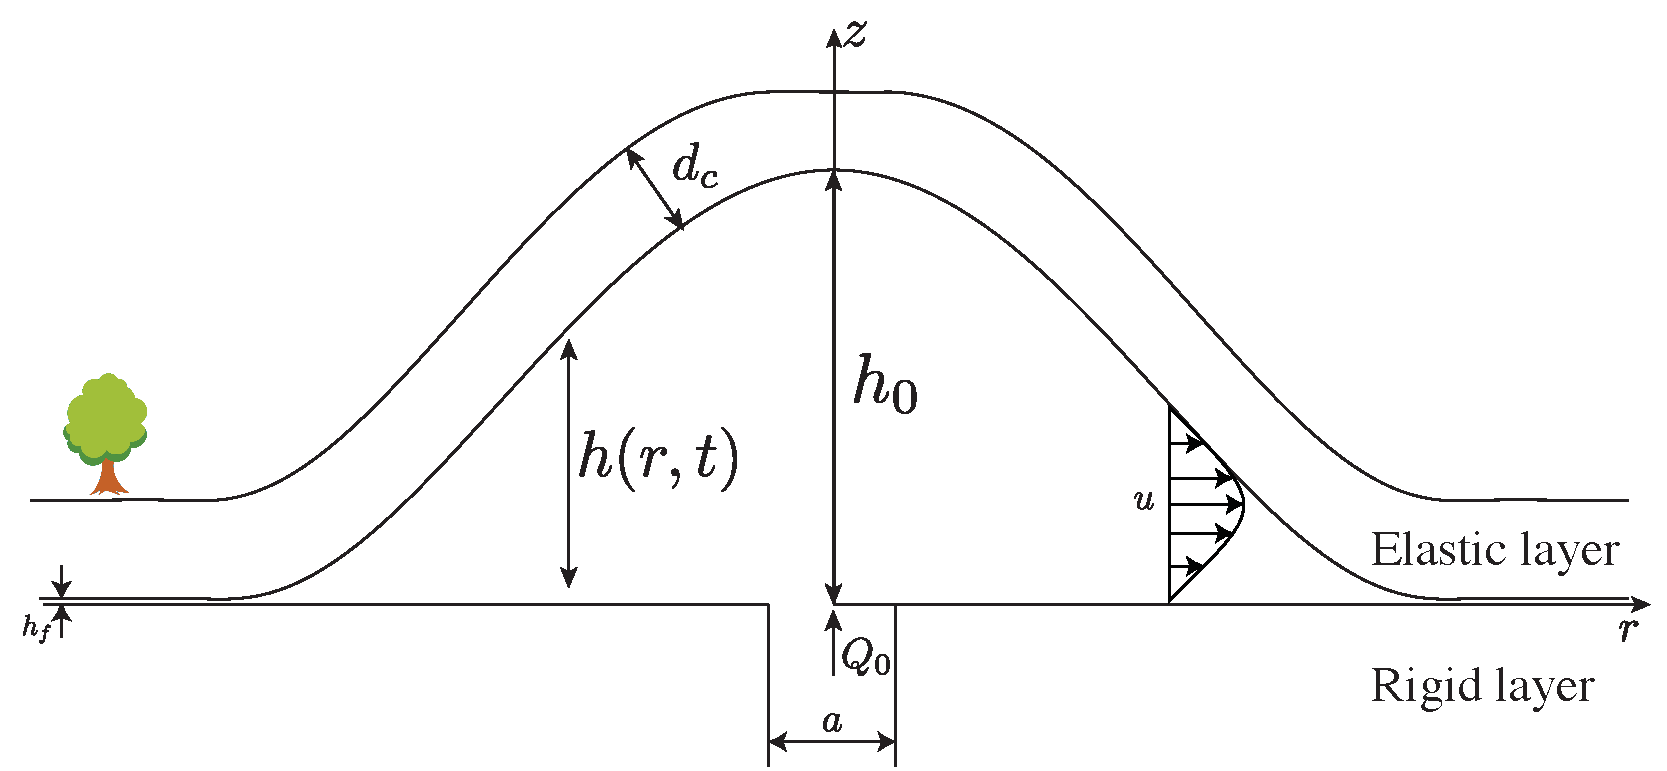
\includegraphics[scale=0.40]{C2_Sketch.pdf}
    \caption{Model geometry and parameters.}
    \label{C2-Sketch}
  \end{center}
\end{figure}

\subsection{Governing equation}
\label{C2-sec:Governing equation}

\textbf{Driving pressure}\\

The  intrusion develops  over a  length scale  $\Lambda$ that  is much
larger than its  thickness $H$ ($\epsilon = H/ \Lambda<<  1$).  In the
laminar  regime  and  in  axisymmetrical  coordinates  ($r$,$z$),  the
Navier-stokes equations within the lubrication assumption are
\begin{eqnarray}
  -\frac{\partial P}{\partial r}  +  \frac{\partial}{\partial z}\left(\eta \frac{\partial u}{\partial z}\right) &=&0\label{C2_V1} \\
  -\frac{\partial P}{\partial z}  - \rho_{m}g&  =&0\label{C2-Npressure}
\end{eqnarray}
where  $u(r,z,t)$  is  the  radial   velocity,  $g$  is  the  standard
acceleration due to gravity and  $P(r,z,t)$ is the pressure within the
fluid.   Integration  of  (\ref{C2-Npressure}) thus  gives  the  total
pressure  $P(r,z,t)$ within  the flow.   When the  vertical deflection
deflection $h(r,t)$  of the upper  elastic layer is small  compared to
its thickness  $d_c$, i.e $h<<d_c$,  we can neglect stretching  of the
upper layer and only consider  bending stresses.  Therefore, the total
pressure $P(r,z,t)$ at a level $z$ in the intrusion is the sum of four
contributions: the  weight of the  magma and  of the upper  layer, the
bending pressure $P_b$ and the atmospheric pressure $P_0$
\begin{equation}
  P = \rho_m g (h-z)+\rho_rgd_c+P_b+P_0
  \label{C2-pression}
\end{equation}
where $h(r,t)$ is the intrusion  thickness and $\rho_r$ the density of
the surrounding rocks. The bending pressure  is given by the force per
unit area  that is necessary  for a  vertical displacement $h$  of the
thin elastic plate \citep{Turcotte:1982ca}
\begin{equation}
  P_d = D\nabla^4h
\end{equation}
where $D$  is the flexural  rigidity of  the thin elastic  layer, that
depends on the Young's modulus $E$, Poisson's ratio $\nu^*$ and on the
elastic           layer          thickness           $d_c$          as
$D = Ed_c^3/\left(12(1-\nu^*)\right)$.

\vspace{.5cm} \textbf{Velocity field} \vspace{.5cm}

At the contact with the elastic sheet $z=h(r,t)$, the no-slip boundary
condition is present  and so, the tangential velocity is  zero and the
normal velocity  is the change  in height ($\partial h/  \partial t$).
With $\vec{n}$ the normal to the surface and $\vec{t}$ the tangent, we
have
\begin{eqnarray}
  \vec{n} \cdot (u,w) &=& \frac{\partial h }{\partial t}\\
  \vec{t} \cdot (u,w) &=& 0 \label{tangeant}.
\end{eqnarray}
The  tangent  vector is  $\vec{t}  =  (1,  \partial h/  \partial  r)$.
However, within the lubrication  assumption, the vertical component of
the  tangent  vector scales  as  $\epsilon$  and thus,  is  negligible
compared to  the radial  component. Therefore, the  boundary condition
($\ref{tangeant}$) reduces  to $u(r,z=h,t)  =0$.  At  the base  of the
flow, the same boundary condition hold and $u(r,z=0,t) =0$.

Equation (\ref{C2_V1}) is integrated twice  as a function of $z$ using
these boundary conditions and the horizontal velocity is
\begin{equation}
  u(r,z,t) =\frac{1}{2\eta} \frac{\partial P}{\partial r} \left(z^2-hz\right)
  \label{C2-vel}
\end{equation}

\vspace{.5cm} \textbf{Injection rate} \vspace{.5cm}

The effective overpressure $\Delta P^*$ driving the flow in the feeder
conduit decreases as the intrusion thickens and is given by
\begin{equation}
  \Delta P^* = \Delta P -\rho_m g h_0 \label{C2-Q0}
\end{equation}
where $h_0(t)$ is the maximum  intrusion thickness at the center $r=0$
and $\Delta P$ is the initial  driving pressure or the overpressure at
the base of the dyke ($z = -Z_c$).

In (\ref{C2-Q0}), the bending pressure  at then center, which scale as
D$h_0(t)/R(t)^4$  where  $R(t)$  is   the  blister  radius,  has  been
neglected.  Although  it tends  to infinity at  the initiation  of the
flow, it rapidly  vanishes as the blister spreads  and the hydrostatic
pressure $\rho_m g h_0$ becomes  the main contribution to the pressure
at the  center.  In addition, the  model assumes a large  aspect ratio
for the blister and does not consider the initiation of the flow.

Finally,  assuming a  Poiseuille flow  within the  cylindrical feeding
conduit, the vertical injection velocity $w_i(r,t)$ and injection rate
$Q(t)$ are given by
\begin{equation}
  w_i=
  \begin{cases}
    \frac{ \Delta P^*}{4 \mu Z_{c}} (\frac{a^{2}}{4}-r^{2})& r \le \frac{a}{2}\\
    0 & r > \frac{a}{2}
  \end{cases}
  \label{C2-eq12}
\end{equation}
\begin{equation}
  Q = Q_0(1-\frac{\rho_m g h_0}{\Delta P})
  \label{C2-eq11}
\end{equation}
where
$Q_0=\left(\pi \Delta P^* a^{4}\right)/\left(128 \eta Z_c\right)$.

\vspace{.5cm} \textbf{Mass conservation} \vspace{.5cm}

The fluid  is assumed  incompressible and a  global statement  of mass
conservation gives
\begin{eqnarray}
  \frac{\partial         h}{\partial        t} +\frac{1}{r}
  \frac{\partial}{\partial
  r} \left( r\int_0^hudz\right) = w_i
  \label{C2-Mass}
\end{eqnarray}
and using (\ref{C2-vel}), we find  that the equation for the evolution
of the thickness in time and space reads
\begin{equation}
  \frac{\partial h}{\partial t} =\frac{\rho_mg}{12 \eta r}
  \frac{\partial}{\partial r}  \left( rh^3  \frac{\partial h}{\partial
      r}\right)+\frac{D}{12\eta r} \left( rh^3 \frac{\partial}{\partial r}\nabla^4h\right)+
  w_i .\label{C2-Heq}
\end{equation}
It is  composed of three different  terms on the right  hand side. The
first term represents gravitational  spreading, i.e.  spreading of the
blister under its own weight. The second term represents the squeezing
of the  flow by the upper  elastic layer.  Both term  are negative and
induces spreading.   The last term  represents fluid injection  and is
positive.

\subsection{Dimensionless equations}
\label{C2-sec:dimens-equat}

Equations  (\ref{C2-eq12}) and  (\ref{C2-Heq}) are  nondimensionalized
using a  horizontal scale $\Lambda$, a  vertical scale $H$ and  a time
scale $\tau$ given by
\begin{eqnarray}
  \Lambda &=& \left(\frac{D}{\rho_m g}\right)^{1/4}\label{L1}\\
  H&=&\left       (\frac{12\eta      Q_{0}}{\rho_{m}g       \pi}\right      )
       ^{\frac{1}{4}} \label{H1}\\
  \tau&=&\frac{\pi \Lambda^{2} H}{Q_{0}}\label{T1}
\end{eqnarray}

where scales  are chosen  such that $Q_0  = \pi\Lambda^2  H/\tau$. The
length scale $\Lamba$ represents the  flexural wavelength of the upper
elastic layer,  i.e. the  length scale at  which bending  stresses and
gravity  contributes equally  to flow.   The height  scale $H$  is the
thickness of  a typical gravity current  and the time scale  $\tau$ is
the  characteristic time  to  fill  up a  cylindrical  flow of  radius
$\Lambda$ and thickness  $H$ at constant rate $Q_0$.   In addition, we
can       define        a       horizontal        velocity       scale
$U=\Lambda/\tau=\left(\rho_m           g           H^3\right)/\left(12
  \eta_h\Lambda\right)$.

The dimensionless equation is
\begin{eqnarray}
  \frac{\partial h}{\partial t}& =&\frac{1}{ r}
                                    \frac{\partial}{\partial r}  \left( rh^3  \frac{\partial h}{\partial
                                    r}\right)+\frac{1}{ r} \left( rh^3
                                    \frac{\partial}{\partial
                                    r}\nabla^4h\right)\nonumber\\
                               &+&
                                   \frac{32}{\gamma^{2}}\left(\frac{1}{4}-\frac{r^{2}}{\gamma^{2}}\right)\left(1-\frac{h_0}{\sigma}\right)
                                   \label{C2-mainEq}
\end{eqnarray}
where the last term is replaced by zero for $r>\gamma/2$. $\gamma$ and
$\sigma$ are  two dimensionless numbers  that control the  dynamics of
the flow
\begin{eqnarray}
  \gamma &=& \frac{a}{\Lambda}\\
  \sigma &=& \frac{\Delta P}{\rho_m g h}.
\end{eqnarray}
$\gamma$  is the  dimensionless radius  of  the conduit,  it does  not
significantly influence the flow and is set to $0.02$ in the following
\citep{Michaut:2009jx,Michaut:2011kg}.   $\sigma$  is  the  normalized
pressure  head,  i.e.,  the  ratio between  the  initial  overpressure
driving the flow and the weight of the magma at the center.
	 
\subsection{Need for regularization}
\label{C2-sec:need-regularization}

One  of   the  main   mathematical  difficulty  in   solving  equation
(\ref{C2-mainEq}) arises at the  contact line.  Indeed, the assumption
that the  thickness of  the fluid  tends to zero  at the  contact line
leads       to       divergent      viscous       stresses,       i.e.
$\eta  \partial   u/\partial  z\rightarrow  \infty$  and   hence,  the
theoretical         immobility          of         the         blister
\citep{Flitton:1999iv,Lister:2013ia,Anonymous:QWXp_4JV}. This problem,
known  a  the  contact-line  paradox,  is  a  well  know  problem  for
surface-tension driven flow  such as the spreading of  a water droplet
\citep{Bertozzi:1998wz,Snoeijer:2013cm}.

The formal proof  have been derived by  \citet{Flitton:1999iv} and can
be derived  as follow. Suppose  that (\ref{C2-mainEq}) has  a solution
and the solution has the  form $h \sim A(t)(R(t)-r)^{\alpha}$ near the
contact line.  As $r \rightarrow R(r)$, the bending term dominates the
gravitational term and (\ref{C2-mainEq}) reduces to
\begin{eqnarray}
  \frac{\partial       h}{\partial       t}&      =&\frac{1}{       r}
                                                     \frac{\partial}{\partial r}\left( rh^3 \frac{\partial}{\partial r}\nabla^4h\right).
                                                     \label{C2-mainEq2}
\end{eqnarray}
Injecting the  solution into  (\ref{C2-mainEq2}) and keeping  only the
leading powers of $R-r$ gives
\begin{eqnarray}
  \frac{\partial    R}{\partial    t}    A\alpha\left(R-r\right)^{\alpha-1}+
  \frac{\partial           A}{\partial           t}\left(R-r)^{\alpha}
  &=&A^4\alpha(\alpha-1)(\alpha-2)\nonumber\\
  &&(\alpha-3)(\alpha-4)(\alpha-5)(R-r)^{4\alpha-6}\nonumber
\end{eqnarray}
The time derivative is locally dominated by its convective part at the
tip, the second  term on the left  is small compared to  the first and
therefore,   by   equating   the   exponent  of   $R-r$,   we   obtain
$\alpha = 5/3$, and by equating the coefficients, we deduce
\begin{equation}
  \frac{\partial R}{\partial r} =-\frac{280}{243} A^3.
\end{equation}
It shows that (\ref{C2-mainEq}) can  only have retreating contact line
($dR/dt<0$)   but  not   with  advancing   contact  line   ($dR/dt>0$)
\citep{Lister:2013ia,Flitton:1999iv}.

To  mitigate this  problem,  one  common approach  is  to  add a  thin
prewetting film, with thickness $h_f$ such that $h\rightarrow h_f$ as
$r\rightarrow  \infty$.   While  the  solution will  depend  upon  the
prewetting  film thickness  $h_f$ and  will not  show any  convergence
properties when $h_f\rightarrow 0$, we will see that the dependence in
$h_f$ is  weak and the  difference between different values  for $h_f$
will  be  relatively  small  \citep{Lister:2013ia,Anonymous:QWXp_4JV}.
Unless otherwise specified, we will consider $h_f = 5\cdot 10^{-3}$ in
the manuscript.



\section{Results}
\label{C2-sec:regime-propagations}

For  a  small  prewetting   film  thickness,  i.e.   $h_f/H<<1$,  the
numerical  resolution of  the  equation  (\ref{EqFinal1}) shows  three
spreading regimes:  a bending  regime where  gravity is  negligible, a
viscous  gravity current  regime  where bending  is  negligible and  a
regime               of              lateral               propagation
\citep{Michaut:2011kg,Bunger:2011cb,Lister:2013ia}.

\begin{figure}[h!]
  \begin{center}
    \graphicspath{ {/Users/thorey/Documents/These/Manuscript/Figure/Chapter2/} }
    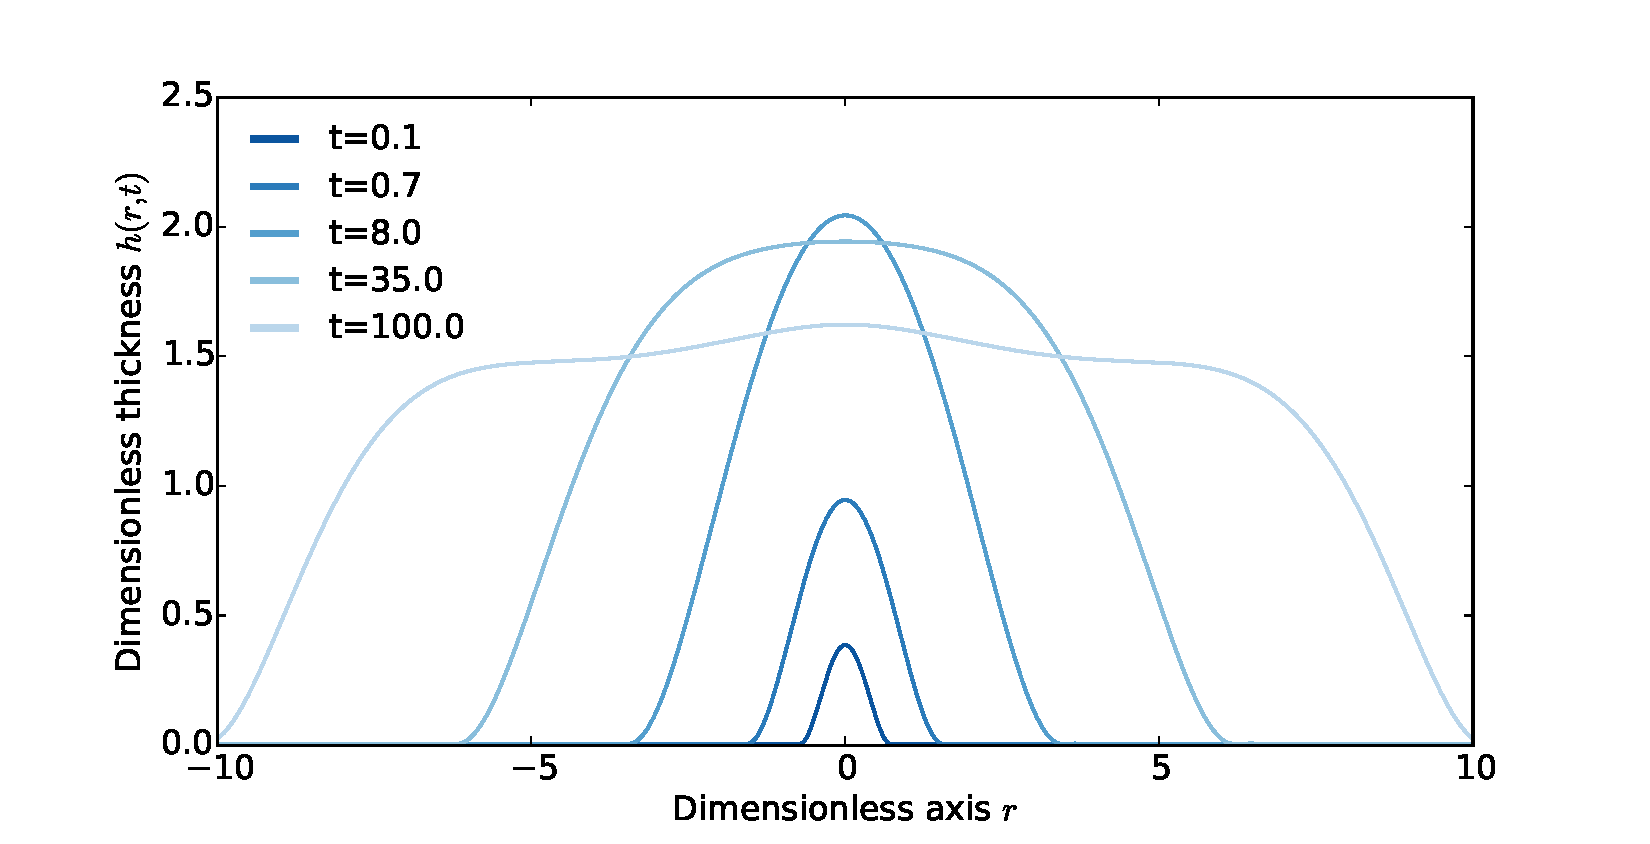
\includegraphics[scale=0.5]{C2_ELAS_GRAV_Profil.eps}
    \caption{Shape of the flow, i.e.  thickness $h(r,t)$ as a function
      of the radial axis $r$ at  five different times indicated on the
      plot. Variables are  dimensionless and one needs  to multiply by
      the characteristic  scales (thickness,  length or time  given by
      (\ref{H1}),  (\ref{L1})  or  (\ref{T1})) to  obtain  dimensional
      values.   For $t<10$,  the intrusion  is in  the bending  regime
      whereas  for $t>10$  the  intrusion is  in  the gravity  current
      regime.}
    \label{C2_ELAS_GRAV_Profil}
  \end{center}
\end{figure}

\subsection{Bending regime}
\label{C2-sec:bending-regime}

At  early times,  when  $R<<\Lambda$, gravity  is  negligible and  the
dynamics of  the spreading  is governed  by the  bending of  the upper
layer.   In addition,  if $h_0<<\sigma$,  the overpressure  $\Delta P$
driving the flow is much larger than  the weight of the blister at the
center and the injection rate can be considered constant.

In that case, the spreading is  very slow and the interior has uniform
pressure $P =\nabla^4h$.  The flow is bell-shaped and its thickness is
given by
\begin{equation}
  h(r,t) = h_0(t)\left(1-\frac{r^2}{R^2(t)}\right)^2
  \label{IntrusionShape}
\end{equation}
with  $h_0(t)$   the  thickness  of   the  intrusion  at   the  center
\citep{Michaut:2011kg,Lister:2013ia}.       In       this      regime,
\citet{Lister:2013ia} have  shown that the spreading  is controlled by
the propagation  of a peeling by  bending wave at the  intrusion front
with dimensionless velocity $c$
\begin{equation}
  c=    \frac{\partial             R}{\partial            t}             =h_f^{1/2}
  \left(\frac{\kappa}{1.35}\right)^{5/2}
  \label{WaveVelocity}
\end{equation}
where  $\kappa  =  \partial^2  h/\partial r^2$  is  the  dimensionless
curvature  of  the  interior  solution.   Using  the  propagation  law
(\ref{WaveVelocity})   and  the   form   of   the  interior   solution
(\ref{IntrusionShape}), they  find that the  radius and the  height of
the intrusion are given by similarity solutions
\begin{eqnarray}
  R(t) &=& 2.2h_f^{1/22}t^{7/22}\label{ScalingR}\\
  h_0(t)&=&0.7 h_f^{-1/11}t^{8/22}\label{ScalingH}.
\end{eqnarray}
where the numerical pre-factor have been matched to our simulations.

\begin{figure}
  \begin{center}
    \graphicspath{ {/Users/thorey/Documents/These/Manuscript/Figure/Chapter2/} }
    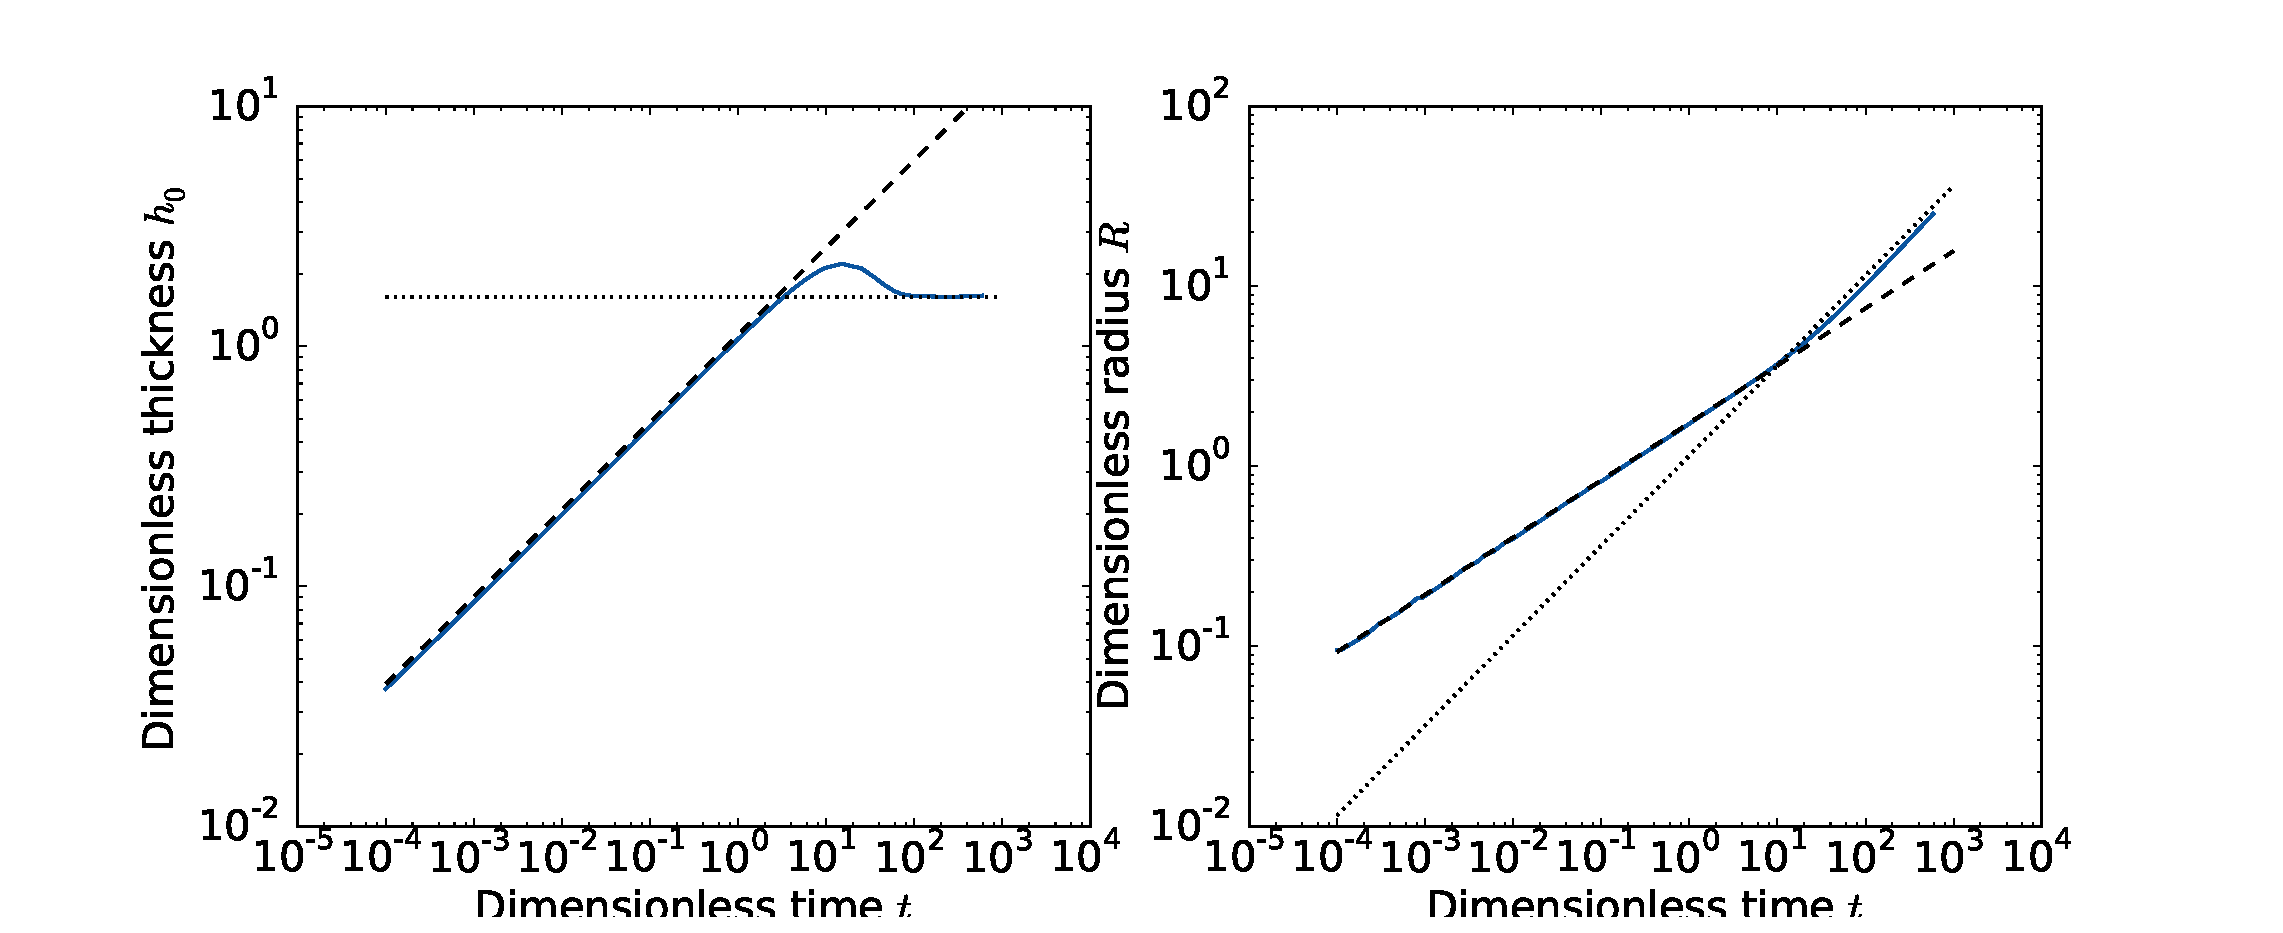
\includegraphics[scale=0.4]{C2_ELAS_GRAV_Sigma.eps}
    \caption{Left: Dimensionless thickness at  the center $h_0$ versus
      dimensionless  time  $t$   for  different  dimensionless  number
      $\sigma$  indicated on  the  plot.   Dashed-lines represent  the
      scaling  laws in  the different  regimes.  Right:  Dimensionless
      radius  $R$   versus  dimensionless   time  $t$  for   the  same
      dimensionless  number  $\sigma$.    Dashed-lines  represent  the
      scaling laws in the different regimes.}
    \label{C2_ELAS_GRAV_Sigma}
  \end{center}
\end{figure}

\subsection{Gravity current regime}
\label{C2-sec:grav-curr-regime}

In  contrast, when  the radius  R becomes  much larger  than $\Lambda$
($R>>\Lambda$), the weight of the  intrusion becomes dominant over the
bending  terms.  The  pressure is  given by  the hydrostatic  pressure
$P = h$  and the intrusion enters a classical  viscous gravity current
regime where bending terms only affect the solution near the intrusion
edge   \citep{Huppert:1982a,Michaut:2011kg,Lister:2013ia}.   In   this
second regime, the radius evolves as $t^{1/2}$ and the thickness tends
to a constant
\begin{eqnarray}
  R(t) &=& 0.715 t^{1/2}\label{Scaling-R-Gravi}\\
  h_0 &=& 1.86\label{Scaling-H-Gravi}
\end{eqnarray} 

\subsection{Lateral propagation}
\label{sec:lateral-propagation}

Once $h_0\rightarrow \sigma$,  the flow is thick  enough to compensate
for  the initial  overpressure. The  thickness at  the center  remains
constant and  the flow enters  a regime of lateral  propagation, where
only its radius $R(t)$ is  to increase \citep{Michaut:2011kg}. In this
regime, except at the center when it redistributes the pressure over a
length scale $\Lambda$, the bending term is negligible compared to the
gravitational  term. \citet{Michaut:2011kg}  has  shown  that in  this
regime, the thickness is constant and the radius evolves as $t^{1/4}$
\begin{eqnarray}
  R(t) &=& \left(\frac{\sigma^3 t}{4\pi}\right)^{1/4}\label{Scaling-R-Propa}\\
  h_0 &=& \sigma\label{Scaling-H-Propa}
\end{eqnarray} 

\section{Application to the spreading of magmatic intrusions}
\label{C2-sec:appl-earth-moon}

\subsection{Earth : Observation Vs Prediction}
\label{sec:observ-vs-pred}

\vspace{.5cm} \textbf{Dataset} \vspace{.5cm}

\citet{E:2015tl}  has made  an extensive  catalog of  $900$ laccoliths
across the  world.  In  particular, \citet{E:2015tl} provides  for the
thickness and  the radius  of $168$ laccoliths  among which,  $40$ are
also  given  with  an  estimation   of  the  intrusion  depth.   These
laccoliths, who are felsic in composition, show thicknesses that range
mainly from $100$ meters to $10$ km with radii in between $1$ and $10$
km.   While  most  of  the  data  are  located  in  the  United  State
($\sim 90\%$),  the different laccoliths  are widely spread  among the
territory and variation in the parameters between different laccoliths
is most likely to be important.
\begin{figure}[h!]
  \begin{center}
    \graphicspath{ {/Users/thorey/Documents/These/Manuscript/Figure/Chapter2/} }
    \includegraphics[scale=0.35]{C2_Geological_Data.eps}
    \caption{a):  Cross section  of  western and  central Elba  Island
      where we can  see the christmas tree structure  of the laccolith
      complex and the main laccolith  units visible at the surface. b)
      Thickness  versus radius  of the  different laccolith  units. c)
      Sketch of the corresponding  location of these laccoliths within
      the    christmas   tree    structure    shortly   after    their
      formations. Figure modified from \citet{Rocchi:2002jy}.}
    \label{C2_Geological_Data}
  \end{center}
\end{figure}

Therefore,  in addition  to the  data from  \citet{E:2015tl}, we  also
consider in this  study the data provided  by \citet{Rocchi:2002jy} on
$9$ laccoliths  nested in a  christmas tree structure at  Elba Island,
Italy  (Figure \ref{C2_Geological_Data}).   The  detailed mapping  and
reconstruction  of  tectonic  history  made  by  \citet{Rocchi:2002jy}
provides for the  parameters of each intrusive layer  in the laccolith
complex. In  addition, for this dataset,  each laccolith is part  of a
larger intrusive system, and hence variability of the model parameters
should be limited,  except for the overlying  elastic layer thickness,
taken to be the intrusion depth, whose variation between laccoliths is
given by  \citet{Rocchi:2002jy}.  The  dispersion is much  smaller for
this dataset; the radius ranges from  $1$ to $10$ km and the thickness
from $40$m to $1$ km.

Finally, we  also account for  $25$ large mafic sills  whose thickness
and radius are given by \citet{Cruden:tg}. In order to account for the
intrinsic scale of  different settings for each  intrusion and compare
them to the model, the data  have first to be nondimensionalized using
characteristic  values for  each intrusion  parameters and  also their
depth, when absent from the catalog.


\begin{figure}[h!]
  \begin{center}
    \graphicspath{ {/Users/thorey/Documents/These/Projet/Refroidissement/Skin_Model/Figure/Figure_Data/} }
    \includegraphics[scale=0.45]{Data_All_Squared.eps}
    \caption{a)  Thickness $h_0$  (m) versus  the radius  $R$ (m)  for
      magmatic  intrusions from  different datasets  indicated on  the
      plot. b) Dimensionless thickness  as a function of dimensionless
      radius, characteristic thickness, and length are calculated from
      (\ref{H1}) and (\ref{L1}).  Dashed  lines: predicted scaling law
      from  the simulations  (black) and  best fit  for the  power law
      $h_0=aR^b$ for each dataset  obtained from a linear least-square
      regression in log-log space.   We use $\rho_m=2500$ kg m$^{-3}$,
      $Q_0  =0.1$ m$^3$  s$^{-1}$ and  $\eta_h=10^6$ Pa  s for  felsic
      laccoliths  and  $\rho_m=3000$  kg   m$^{-3}$,  $Q_0  =1$  m$^3$
      s$^{-1}$  and  $\eta_h=1$ Pa  s  for  their mafic  counterparts.
      Unless  the intrusion  depth is  given  by the  dataset, we  use
      $d_c=1500$ m and $g=9.81$ m s$^{-2}$.  c) and d), same plots but
      where we compared the laccoliths from \citep{Rocchi:2002jy} to a
      set of  low-slope domes  given by  \citet{Wohler:2009jj}.  Lunar
      domes   are  nondimensionalized   using  $g=1.62$   m  s$^{-2}$,
      $\rho_m=3000$ kg  m$^{-3}$, $Q_0 =1$ m$^3$  s$^{-1}$, $\eta_h=1$
      Pa s  and $d_c$,  which is not  given in the  dataset is  set to
      $1500$ m.  In all cases, the Poisson's ratio is $\nu^*=0.25$.}
    \label{Corry_Rocchie}
  \end{center}
\end{figure}



\vspace{.5cm} \textbf{Range of value for the parameters} \vspace{.5cm}

In terrestrial settings, magma density  $\rho_m$ depends mainly on its
composition and varies between $ 2500$ kg m$^{-3}$ for felsic lavas to
$3000$ kg m$^{-3}$ for a more mafic lavbas.  Reported intrusion depth,
which is set to $1.5$ km otherwise,  varies from $180$ to $2200$ m for
the laccoliths in \citet{E:2015tl} and from  $1.9$ to $3.7$ km for the
laccoliths at Elba Island.  Hence, for a Young's modulus value of $10$
GPa, the characteristic length scale $\Lambda$ varies between $\sim 1$
km and $\sim  7$ km for laccoliths.  The density  does not affect much
the value of  $\Lambda$ and the characteristic length  scale for large
mafic sills,  whose depths are  not reported in  \citet{Cruden:tg} and
set to $1.5$ km, is equal to $\sim 3$ km.

On Earth, laccoliths are generally  formed by relatively evolved lavas
that  may have  differentiated from  primitive magma  in deep  crustal
magma chambers,  located some $5$  to $15$  km below the  surface. The
overpressures  driving magma  ascent are  typically $20$  to $50$  MPa
\citep{Stasiuk:1993kg,Barmin:2002ea},    which   gives    overpressure
gradients  of $\sim  10^3$ Pa  m$^{−1}$.  Lava  viscosity at  eruption
temperature  $\eta_h$  depends mainly  on  its  composition and  water
content; close to its liquidus  temperature, it can varies from $10^2$
Pa  s   for  mafic   lavas  to   $10^{5}$  Pa   s  for   felsic  lavas
\citep{Anonymous:CZVBrBvv,Giordano:2008em,Whittington:2009fv,Chevrel:2013jn}.
\citet{Wada:2007tv} show  that the dyke  width tends to  increase with
viscosity  to the  power $1/4$  \citep{Kerr:1995tl}; mafic  lavas with
viscosity $10^2$ Pa s at eruption  temperature tend to form dyke $1$ m
wide, while felsic  magmas, with viscosities of $10^6$-$10^7$  Pa s at
eruption temperature, tend  to form dykes $100$ m wide.   For the same
overpressure   gradient,  plugin   in   these   parameters  in   $Q_0$
(\ref{C2-eq11}) gives an injection rate  close to $0.1$ m$^3$ s$^{-1}$
for mafic  lavas and $2.5~10^3$  m$^3$ s$^{-1}$ for felsic  lavas. The
height scale $H$ is thus $\sim 25$ for felsic laccolith and $\sim 0.1$
m for large mafic sills.

\begin{table}[h!]
  \caption{Range of values for the model parameters}
  \centering
  \begin{tabular}{c|c|c|c|c}
    Parameters& Symbol & Earth & Moon&Unit\\
    \hline
              &&&&\\
    Depth of intrusion & $d_c$ & $0.2-2.7$ &$0.1-5$ &km \\
    Young's Modulus & $E$ & $10$ &$10-100$ &GPa \\
    Poisson's ratio & $\nu^*$ & $0.25$ &$0.25$ &\\
    Gravity & $g$ & $9.81$ &1.62&m s$^{-2}$ \\
    Crust density & $\rho_{r}$ & $2500$ &$2500$&kg m$^{-3}$ \\
    Magma density & $\rho_{m}$ & $2500-3000$ &$3000$&kg m$^{-3}$ \\
    Magma viscosity & $\eta_h $ & $10^2-10^{4}$ &$1-10^{2}$&Pa s \\
    Feeder dyke width & $a$ & $1-100$ &$1-10$&m \\
    Depth of the melt source & $Z_{c}$ & $ 1-10$&$200-500$& km \\ 
    Initial overpressure & $\Delta P$ & $20-50$ &$1-5$ &MPa \\
    Injection rate & $Q_{0}$ &$0.1-10^3$ &$1-10$&m$^{3}$ s$^{-1}$ \\
              &&&&\\
    \hline
    Characteristic scales & Symbol & Earth & Moon&Unit\\
    \hline
              &&&&\\
    Height scale & $H$& $0.1-25$ &$0.1-1$ &m \\
    Length scale & $\Lambda$ & $1-7$&$1-20$& km \\
    Time scale & $\tau$ & $10^{-1}-10$&$10^{-2}-1$& years \\
    \label{tab2}
  \end{tabular} 
\end{table}

The model  also considers  a thin pre-wetted  film of  thickness $h_f$
whose  meaning in  the application  to the  spreading of  laccolith is
unclear.  In  particular, the  model shows  no convergence  when $h_f$
tends to zero \citep{Lister:2013ia} and therefore, the thickness $h_f$
might be  linked to some structural  length scale at the  front of the
laccolith or  to the natural  imperfection of the flow  geometry.  For
the purpose of the application, we  choose a film thickness of $1$ mm,
i.e.  the  minimum length  scale with  physical signification  for the
spreading of laccoliths  which give a dimensionless  $h_f$ that varies
between $10^{-2}$  and $10^{-4}$.  In  the following, we set  $h_f$ to
$10^{-3}$.

\vspace{.5cm}  \textbf{Dimensionless  data  and  comparison  with  the
  model} \vspace{.5cm}

Each  magmatic   intrusion  unit  is  made   dimensionless  using  its
characteristic  length   scale  $\Lambda$,  which  depends   upon  the
intrusion depth, and its characteristic  height scale, which is either
$H=25$  m for  felsic laccolith  or $H=0.1$  m for  large mafic  sills
(Figure  \ref{Corry_Rocchie}).   First,  the dimensionless  radius  of
laccoliths at  Elba Island and  $95\%$ of those  from \citet{E:2015tl}
are  smaller than  $4$ consistent  with  their arrest  in the  bending
regime. The prediction of the model for the evolution of the thickness
$h_0$ of  the current as  a function of its  radius $R$ can  be easily
derived from  the scaling  laws (\ref{ScalingH})  and (\ref{ScalingR})
and should follow
\begin{equation}
  h_0 \sim 0.3h_f^{-1/7} R^{8/7}\label{C2-Hr}
\end{equation}
in agreement  with the  power law relationship  $h_0 =  bR^a$ proposed
initially         by         \citet{McCaffrey:1997ea}         (Section
\ref{sec:empl-dynam-des}).   To characterize  the mean  trend in  each
population, we make use of a linear least-square regression in log-log
space to obtain a value for the  coefficient $a$ and $b$ that best fit
the  observation.   We  found  $h_0  = 21  R^{1.22\pm  0.1}$  for  the
laccoliths at Elba island which  is very close to $R^{1.14}$ predicted
by the model (Figure  \ref{Corry_Rocchie}).  Actually, the geometry of
these  laccoliths  is  not  well  known  and  probably  not  perfectly
axisymmetric.   \citet{Anonymous:QWXp_4JV}   found  that  for   a  two
dimensional flow,  $h_0\propto \delta^{1/7}L^{1.42}$ where $L$  is the
half-length of the  flow.  The best fit value for  the coefficient $a$
then nicely inserts between the expected values for the two geometries
as noted  by \citet{Michaut:2011kg}.  In contrast,  the prediction for
the coefficient  $b$ is much  smaller than the predicted  value.  Even
for $h_f=10^{-2}$, which  would be an upper bound  for this parameter,
the  model  predict $b=0.15$,  which  is  three orders  of  magnitudes
smaller than  the observation (Figure  \ref{Corry_Rocchie}).  Matching
the data to the model will  require using a viscosity $\eta_h$ for the
magma  abnormally   high,  i.e.   $\eta_h   \sim  10^{12}$  Pa   s  or
unreasonable injection rate, i.e. $Q_0\sim 1$ km$^3$ s$^{-1}$.

The  best  fit   power  law  relationship  for   the  laccoliths  from
\citep{E:2015tl}   is   $h_0   =    21   R^{0.62\pm   0.08}$   (Figure
\ref{Corry_Rocchie}).  In that case, the  exponent $a$ is smaller than
one and  does not agree with  the model. This value,  which is smaller
than the  previous value proposed for  $a$ by \citet{McCaffrey:1997ea}
and calculated directly on the data, was interpreted as reflecting the
two stage  growth process  historically invoked  for the  formation of
laccolith (Section \ref{sec:empl-dynam-des}).  However, the dispersion
in  the  data   is  much  important  than  in   the  observation  from
\citet{Rocchi:2010dn}   and   not   taken    into   account   in   the
nondimensionalization which  assumes the  same parameters for  all the
different laccoliths.

Half of the  large mafic sills show dimensionless  radius smaller than
$R=4$, not consistent with their  arrest in the gravity current regime
(Figure  \ref{Corry_Rocchie}).    In  addition,   their  dimensionless
thickness, which  should tend to  a constant  of order $O(1)$  is much
larger than the expected value and increases with the radius $R$.  For
a  gravity current  in a  two dimensional  geometry, the  thickness is
indeed  expected to  increase  with the  length of  the  sill, but  as
$L^{1/4}$ \citet{Michaut:2011kg}  which is much weaker  than the found
value for the  coefficient $a$ of $0.76$ for large  mafic sill (Figure
\ref{Corry_Rocchie}).

\subsection{Origin of lunar low-slope domes}
\label{sec:observ-vs-pred}


\section{Discussion}
\label{C2-sec:discussion}


\bibliographystyle{agufull08}
\bibliography{/Users/thorey/Dropbox/Library}



%%% Local Variables:
%%% mode: latex
%%% TeX-master: "../main"
%%% End:


\part{Theoretical  model for  the  cooling  of elastic-plated  gravity
  current and applications to laccolith on the Earth and Moon}

\addtocontents{toc}{\setcounter{tocdepth}{-1}}
\chapter{Elastic-plated gravity current with temperature-dependent viscosity} 
\label{C3-JFM} 
\minitoc

\begin{abstract}
  Temperature-dependent elastic-plated gravity  currents have numerous
  applications in nature, from shallow magmatic intrusions to the flow
  of melt-water below  an ice sheet. We develop  the general equations
  for an  elastic-plated gravity current with  a temperature-dependent
  viscosity for constant influx conditions.  We show that the coupling
  between  the  thermal  structure  and the  flow  itself  results  in
  important deviations  from the  isoviscous case. In  particular, the
  bending  and  gravity  asymptotic  regimes,  characteristic  of  the
  isoviscous  case,  both  split  into three  phases:  a  first  'hot'
  isoviscous phase, a second phase  where the flow effective viscosity
  and  thickness drastically  increase and  a third  'cold' isoviscous
  phase.  These three  phases  are  controlled by  the  extent of  the
  thermal anomaly, for  which we develop analytical  scaling laws. The
  effective flow viscosity  is governed by the local  thermal state at
  the current tip  in the bending regime while it  is the average flow
  viscosity in the gravity regime.  In the end, the complete evolution
  of such  an elastic-plated  gravity current  depends on  its thermal
  state at the transition between  the bending and gravity regimes. We
  provide  a  phase diagram  which  predicts  the different  evolution
  scenarios  as a  function of  the flow  Peclet number  and viscosity
  contrast.

\end{abstract}


\section{Introduction}

Elastic-plated  gravity  currents  involve the  spreading  of  viscous
material beneath  an elastic  sheet. The  applications range  from the
emplacement      of      lava      in      the      shallow      crust
\citep{Michaut:2011kg,Bunger:2011cb} and melt-water drainage below ice
sheet  \citep{Das:2008in,Tsai:2010ev}  in  geological setting  to  the
manufacture of flexible electronics and microelectromechanical systems
(MEMS) in engineering \citep{Hosoi:2004dn}.

When  the thickness  of  the flow  is small  compared  to its  extent,
lubrication  approximation applies  and  the  study of  elastic-plated
gravity currents  resumes to  the study of  a sixth  order, non-linear
partial                      differential                     equation
\citep{Michaut:2011kg,Lister:2013ia,Anonymous:QWXp_4JV}   .   However,
the assumption  that the thickness of  the fluid tends to  zero at the
contact  line  leads  to  divergent viscous  stresses,  and  hence,  a
regularization     condition     is     needed    at     the     front
\citep{Flitton:1999iv,Lister:2013ia,Anonymous:QWXp_4JV}.   One  common
approach is to add a thin  prewetting film of fluid, thus avoiding the
requirement  for   any  boundary   conditions  at  the   contact  line
\citep{Lister:2013ia,Anonymous:QWXp_4JV}.

The dynamics  of the spreading  has been described in  an axisymmetric
geometry   for    a   Newtonian   fluid   with    constant   viscosity
\citep{Michaut:2011kg,Lister:2013ia,Thorey:2014cv}   and    show   two
distinct regimes of  evolution.  First, gravity is  negligible and the
peeling of the front is driven  by bending of the overlying layer; the
interior  is bell-shaped,  the radius  evolves as  $t^{8/22}$ and  the
thickness  as  $t^{7/22}$.   When   the  radius  becomes  larger  than
$4\Lambda$, where  $\Lambda$ is the  flexural wavelength of  the upper
layer, the  weight of  the current becomes  dominant over  the bending
terms    and   the    flow   enters    a   gravity    current   regime
\citep{Huppert:1982a}.  In this regime, the thickness profile develops
a flat top with bent edges,  the radius evolves as $t^{1/2}$ while the
thickness  tends to  a  constant.  Different  analogue experiments  of
isoviscous     flows     confirm     these     theoretical     results
\citep{Dixon:1987js,Lister:2013ia}.

However, in  many real geological settings,  the isothermal/isoviscous
assumption  are not  valid.  For  instance, the  viscosity of  magmas,
produced by partial  melting of the upper mantle, can  vary by several
orders    of   magnitude    \citep{Anonymous:CZVBrBvv,Lejeune:1995fc}.
Therefore,  as the  fluid flows,  it cools  down, its  composition and
crystal content change which, in  turn, modifies the viscosity and the
dynamics of the  flow.  Several studies have shown that,  in a gravity
current, this coupling between the cooling and the flow itself results
in     important    deviations     from     the    isoviscous     case
\citep{Bercovici:2007vc,Bercovici:1996uu,BALMFORTH:1999ey,Garel:2014era}.

In  this paper,  we examine  how  the spreading  of an  elastic-plated
gravity current is affected by  the cooling itself.  In particular, we
consider  the  problem  of  an elastic-plated  gravity  current  whose
viscosity depends  on temperature  according to a  prescribed rheology
$\eta(T)$.   This  gives rise  to  a  set  of two  coupled  non-linear
equations  that  we solve  numerically.   We  study the  flow  thermal
structure and its effect on the  dynamics through the rheology in each
regime separately.  In both regimes, we identify different ``thermal''
phases of propagation that we  characterize by different scaling laws.x

\section{Theory}
\label{C3-sec:theory}

\subsection{Formulation}
\label{C3-sec:formulation}

We model  the axisymmetric  flow of  fluid below  an elastic  layer of
constant thickness $d_c$ and above a semi infinite rigid layer (Figure
\ref{C3-Figure2-1}).   The assumption  that  the thickness  of the  fluid
$h(r,t)$ tends to zero at the  contact line leads to divergent viscous
stresses   and  to   the   theoretical  immobility   of  the   current
\citep{Flitton:1999iv}.   To avoid  problem  at the  contact line,  we
consider    a   thin    pre-wetting    film    of   thickness    $h_f$
\citep{Lister:2013ia} (Figure \ref{C3-Figure2-1}).

The  fluid is  injected continuously  at the  base and  center of  the
current  at  a constant  rate  $Q_0$  through  a conduit  of  diameter
$a$. The hot fluid is intruded  at temperature $T_i$ and cools through
the  top and  bottom by  conduction in  the surrounding  medium, whose
temperature is  considered constant  and equal to  $T_0$.  In  using a
fixed temperature at the flow boundary, we essentially assume that the
fluid is bounded by a medium with infinite thermal conductivity.

%% FIGURE 2-1
\begin{figure}
  \begin{center}
    \graphicspath{ {/Users/thorey/Documents/These/Projet/Refroidissement/Skin_Model/Figure/JFM_V13/} }
    \includegraphics[scale=0.28]{ModelGeometry.eps}
    \caption{Model  geometry and  parameters.  The  vertical scale  is
      exaggerated.}
    \label{C3-Figure2-1}
  \end{center}
\end{figure}

As  it  cools,  the  viscosity  of the  fluid  increases  following  a
prescribed temperature-dependent rheology $\eta(T)$ given by
\begin{equation}
  \eta(T)=\frac{\eta_h
    \eta_c(T_i-T_0)}{\eta_h(T_i-T_0)+(\eta_c-\eta_h)(T-T_0)}
  \label{C3-rheology}
\end{equation}
where $\eta_h$  and $\eta_c$  are the viscosities  of the  hottest and
coldest  fluid  at  the   temperature  $T_i$  and  $T_0$  respectively
\citep{Bercovici:2007vc}.    Although   this   rheology   is   largely
simplified,  the  inverse  dependence   of  viscosity  on  temperature
captures  the  essential  behavior  of  a  viscous  fluid,  i.e.   the
viscosity  variations are  the largest  where the  temperature is  the
coldest
\citep{Anonymous:CZVBrBvv,Marsh:1981dc,Lejeune:1995fc,Giordano:2008em}.

\subsection{Pressure}
\label{C3-sec:Pressure}

The  intrusion develops  over a  length scale  $\Lambda$ that  is much
larger than its thickness $H$ ($\Lambda >> H$).  In the laminar regime
and  in   axisymmetrical  coordinates  ($r$,$z$),   the  Navier-Stokes
equations within the lubrication approximaton are
\begin{eqnarray}
  -\frac{\partial P}{\partial r}  +  \frac{\partial}{\partial z}\left(\eta(T) \frac{\partial u}{\partial z}\right) &=&0\label{C3-V1} \\
  -\frac{\partial P}{\partial z}  - \rho_{m}g&  =&0\label{C3-Npressure}
\end{eqnarray}
where $u(r,z,t)$ is  the radial velocity, $\rho_m$  the fluid density,
$g$  the  standard acceleration  due  to  gravity and  $P(r,z,t)$  the
pressure within the fluid.  Integration of (\ref{C3-Npressure}) gives the
total  pressure  $P(r,z,t)$  within   the  flow.   When  the  vertical
deflection $h(r,t)$  of the upper  elastic layer is small  compared to
its thickness  $d_c$, i.e $h<<d_c$,  we can neglect stretching  of the
upper layer and only consider  bending stresses.  Therefore, the total
pressure $P(r,z,t)$ at a level $z$ in  the current is the sum of three
contributions: the weight of the magma  and of the upper layer and the
bending pressure
\begin{equation}
  P = \rho_m g (h-z)+\rho_rgd_c+D\nabla_r^4h
\end{equation}
where  $h(r,t)$ is  the flow  thickness, $\rho_r$  the density  of the
surrounding rocks and $D$ is the flexural rigidity of the thin elastic
layer, that  depends on Young's  modulus $E$, Poisson's  ratio $\nu^*$
and     on     the     elastic    layer     thickness     $d_c$     as
$D = Ed_c^3/\left(12(1-\nu^*)\right)$.

\subsection{Injection rate}

Assuming a Poiseuille flow within the cylindrical feeding conduit, the
vertical injection  velocity $w_i(r,t)$  and injection rate  $Q_0$ are
given by
\begin{equation}
  w_i(r,t)=
  \begin{cases}
    \frac{ \Delta P}{4 \eta_h Z_{c}} (\frac{a^{2}}{4}-r^{2})& r \le \frac{a}{2}\\
    0 & r > \frac{a}{2}
  \end{cases}
  \label{C3-eq12}
\end{equation}
\begin{equation}
  Q_{0}=\frac{\pi \Delta P a^{4}}{128 \eta_h Z_c}
  \label{C3-eq11}
\end{equation}
where  $\Delta P$  is  the  initial overpressure  within  the melt  at
$z=Z_{c}$.

\subsection{Heat transport equation}
\subsubsection{Local energy conservation}

In the laminar regime and in axisymmetrical coordinates ($r$,$z$), the
local energy  conservation equation within the  lubrication assumption
is
\begin{eqnarray}
  \frac{D}{D t}\left(\rho_m C_{p,m} T+\rho_mL(1-\phi)\right)&=& k_m  \frac{\partial^2
                                                                T}{\partial               z^2}\label{C3-EnergyCons}
\end{eqnarray}
where  $T(r,z,t)$ is  the fluid  temperature and  $\rho_m$, $k_m$  and
$C_{p,m}$ are the  density, thermal conductivity and  specific heat of
the   fluid.   Here,   we   also  account   for   energy  release   by
crystallization of the fluid, which is a non negligible source of heat
for magmas; $\phi(r,z,t)$ is the crystal  fraction in the melt and $L$
the latent heat  of crystallization.  In this model,  the crystals are
considered only  as a source/sink  of energy as they  melt/form during
flow emplacement.  In particular, the physical properties of the fluid
are not modified by the presence of crystals.


Following a common approximation, we  assume that the crystal fraction
is a linear function of temperature over the melting interval
\begin{equation}
  \phi = \frac{T_L-T}{T_L-T_s}
  \label{C3-meltfraction}
\end{equation}
where $T_S$ and $T_L$ are the solidus and liquidus temperatures of the
magma \citep{Hort:1997hk,Michaut:2006di}. In  addition, we assume that
the fluid is  injected at its liquidus temperature ,  i.e. $T_L = T_i$
and,  for simplicity,  that the  solidus temperature  is equal  to the
surrounding rock  temperature $T_S  =T_0$. With  these approximations,
the local energy equation (\ref{C3-EnergyCons}) resumes to
\begin{eqnarray}
  \frac{\partial T}{\partial t}+ u\frac{\partial T}{\partial r}
  + w\frac{\partial T}{\partial z}  &=& \frac{ St}{St+1}\kappa_m  \frac{\partial^2
                                        T}{\partial               z^2}
                                        \label{C3-EnergyCons2}
\end{eqnarray}
where  $u(r,z,t)$ and  $w(r,z,t)$ are  the radial  and vertical  fluid
velocities, $St =\left(C_{p,m}(T_i-T_0)\right)/L$ is the Stefan number
and     $\kappa_m$     is     the    fluid     thermal     diffusivity
$\kappa_m = k_m/(\rho_m C_{p,m})$.  We  use an integral balance method
to solve the heat transport equation (\ref{C3-EnergyCons2}).  This theory
is based  on the  integral-balance method  of heat-transfer  theory of
\citet{Goodman:1958ue},  in  which  the   vertical  structure  of  the
temperature field  is represented  by a known  function of  depth that
approximates the expected solution.

\subsubsection{Integral   balance   solution   for   the   temperature
  $T(r,z,t)$}

Following \citet{BALMFORTH:1999ey},  we model the cooling  of the flow
through  the  growth  of  two thermal  boundary  layers:  one  growing
downward from the  top and a second growing upward  from the base.  As
we consider homogeneous thermal  properties for the surrounding rocks,
we assume that the two  thermal boundary layers grow symmetrically and
have the  same thickness  $\delta(r,t)$ (Figure  \ref{C3-Figure2-1}).  We
use the  following approximation for the  vertical temperature profile
$T(r,z,t)$
\begin{equation}
  T=
  \begin{cases}
    T_b - (T_b-T_0)(1-\frac{z}{\delta})^2 & 0 \le z\le \delta \\
    T_b & \delta \le z\le h-\delta \\
    T_b - (T_b-T_0)(1-\frac{h-z}{\delta})^2 & h-\delta \le z\le h\\
  \end{cases}
  \label{C3-Temperature}
\end{equation}
where $T_b(r,t)$  is the temperature at  the center of the  flow.  The
integral balance  solution in  (\ref{C3-Temperature}) assumes  a symmetry
around $z=h/2$  and a decrease of  the temperature in the  two thermal
boundary  layers  down  to  the  surrounding  rock  temperature  $T_0$
\citep{BALMFORTH:1999ey}.    In  addition,   it   assumes  a   uniform
temperature  $T_b$ in  between the  thermal boundary  layers.  As  the
fluid is  injected at  temperature $T_i$, we  have $T_b(r,t)  =T_i$ as
long as  $\delta<h/2$ (Figure  \ref{C3-Figure2-1}).  However, if  the two
thermal boundary layers connect, then $\delta = h/2$ and $T_b\le T_i$.
This profile assures  the continuity of the temperature  and heat flux
within the flow.


\subsubsection{Integral balance equation}
\label{C3-sec:integr-balance-equat}

We  begin  by  integrating  the  local  energy  conservation  equation
(\ref{C3-EnergyCons2}) separately  over the two thermal  boundary layers.
The integration  over the  bottom thermal layer,  i.e. from  the base,
$z=0$ to a level $z = \delta$ gives
\begin{eqnarray}
  &&\frac{\partial}{\partial t}\left( \delta( \bar{T}-T_b)\right)+\frac{1}{r}\frac{\partial}{\partial r} \left( r\delta(\overline{uT}-\bar{u}T_b)\right) + \delta\left( \frac{\partial T_b}{\partial t}+ \overline{u}\frac{\partial T_b}{\partial r}\right)\nonumber\\
  &=&-\frac{\kappa_m}{1+St}\left. \frac{\partial T}{\partial z}\right|_{z=0}+w_{i}(T_{i}-T_b)
      \label{C3-Local1}
\end{eqnarray}
where the bars  indicate the vertical average over  the bottom thermal
boundary layer
\begin{equation}
  \overline{f} = \frac{1}{\delta}\int_0^{\delta}f dz\nonumber,
\end{equation}
which will be determined once the horizontal flow velocity is derived,
$T_b(r,t)$  is  the  temperature  at  $z=\delta$,  $w_{i}(r)$  is  the
vertical  injection velocity  and  we  have used  the  nullity of  the
thermal gradient at $z=\delta$ and the local mass conservation
\begin{equation}
  \frac{1}{r}\frac{\partial ru}{\partial r} +\frac{\partial w}{\partial z}=0.
  \label{C3-MassConservation}
\end{equation}
The  integration over  the top  thermal layer,  i.e., from  the level,
$z=h-\delta$ to the top $z=h$ gives
\begin{eqnarray}
  &&\frac{\partial}{\partial t}\left( \delta( \bar{T}-T_b)\right)+\frac{1}{r}\frac{\partial}{\partial r} \left( r\delta(\overline{uT}-\bar{u}T_b)\right) + \delta\left(\frac{\partial T_b}{\partial t}+ \overline{u}\frac{\partial T_b}{\partial r}\right)\nonumber\\
  &=&\frac{\kappa_m}{1+St^{-1}}\left. \frac{\partial T}{\partial z}\right|_{z=h}
      \label{C3-Local2}
\end{eqnarray}
where,    in    addition    to    the    local    mass    conservation
(\ref{C3-MassConservation})  and the  fact that  the thermal  gradient at
$z=h-\delta$ is  equal to  zero, we have  used the  kinematic boundary
condition in $z=h(r,t)$
\begin{equation}
  \frac{\partial h}{\partial t} +u\frac{\partial h}{\partial
    r} = w.
\end{equation}

Therefore,  the  heat  balance   equation,  i.e.   the  heat  equation
(\ref{C3-EnergyCons2}) integrated over the flow thickness, is obtained by
adding (\ref{C3-Local1})  and (\ref{C3-Local2}).   Using (\ref{C3-Temperature})
to derive the conductive fluxes, we finally obtain
\begin{eqnarray}
  &&\frac{\partial}{\partial t}\left( \delta( \bar{T}-T_b)\right)+\frac{1}{r}\frac{\partial}{\partial r} \left( r\delta(\overline{uT}-\bar{u}T_b)\right) + \delta\left( \frac{\partial T_b}{\partial t}+ \overline{u}\frac{\partial T_b}{\partial r}\right)\nonumber\\
  &=&-\frac{2\kappa_m}{(1+St^{-1})}\frac{\left( T_b - T_0\right)}{\delta}+\frac{w_{i}}{2}(T_{i}-T_b).
      \label{C3-LocalHeat3}
\end{eqnarray}

\subsection{Equation of motion}
\label{C3-sec:equation-motion}

A global statement of mass conservation gives
\begin{eqnarray}
  \frac{\partial h}{\partial t}+ \frac{1}{r}
  \frac{\partial}{\partial
  r} \left( r\int_0^hudz\right)= w_i.
  \label{C3-C3}
\end{eqnarray}
To obtain an  equation for the flow thickness, we  first note that the
chosen vertical structure of the temperature field (\ref{C3-Temperature})
is symmetric  around $h/2$, and  thus, because the  boundary condition
are  the same  at  $z=0$ and  $z=h$, the  viscosity  and velocity  $u$
possess  the same  symmetry.  Taking  advantage of  this symmetry,  we
integrate              once              (\ref{C3-V1})              using
$\left.\frac{\partial u}{\partial z}\right|_{z=h/2}=0$ to get
\begin{equation}
  \frac{\partial   u}{\partial   z}   =   \frac{1}{\eta(z)}\frac{\partial
    P}{\partial r}\left(z-\frac{h}{2}\right).
  \label{C3-deriv}
\end{equation}
Using no-slip  boundary conditions at  the top  and the bottom  of the
flow, i.e.  $u(r,z=0,t)=u(r,z=h,t)=0$, (\ref{C3-C3}) can be rewritten as
\begin{eqnarray}
  \frac{\partial h}{\partial t} = \frac{1}{r}
  \frac{\partial}{\partial
  r} \left( r\int_0^h\frac{\partial u}{\partial z}zdz\right) + w_i.
  \label{C3-Mass}
\end{eqnarray}
Finally,  injecting (\ref{C3-deriv})  into  (\ref{C3-Mass}) gives  the
equation for the flow thickness evolution in axisymmetric coordinates
\begin{eqnarray}
  \frac{\partial h}{\partial t} = \frac{1}{r}
  \frac{\partial}{\partial r} \left( r\left(\rho_m g \frac{\partial h}{\partial      r}+D\frac{\partial}{\partial      r}\left(\nabla_r^4h\right)\right)\left(\int_0^h\frac{1}{\eta(y)}\left(y-\frac{h}{2}\right)ydy\right)\right)
  + w_i.
  \label{C3-Mass-2}
\end{eqnarray}
In  addition,  integration  of   (\ref{C3-deriv})  using  the  no-slip
boundary condition at the base of the flow gives
\begin{equation}
  u(r,z,t)        =        \frac{\partial        P}{\partial        r}
  \int_0^z\frac{1}{\eta(y)}\left(y-\frac{h}{2}\right)dy.
  \label{C3-udimensione}
\end{equation}
where
\begin{equation}
  \frac{1}{\eta(y)} = \frac{1}{\eta_c}+\frac{\eta_c-\eta_h}{\eta_h\eta_c}\frac{T(y)-T_0}{T_i-T_0}.
\end{equation}
$T(y)$    being   a    polynom,   integrals    in   (\ref{C3-Mass-2}),
(\ref{C3-udimensione}) as well as  the averaged quantities $\overline{u}$
and   $\overline{uT}$    over   the   thermal   boundary    layer   in
(\ref{C3-LocalHeat3}) can easily be calculated.

\subsection{Dimensionless equations}
\label{C3-sec:dimens-equat}

We use the characteristic temperature interval $\Delta T = T_i-T_0$ to
nondimensionalize  temperatures.  The  dimensionless integral  balance
approximation (\ref{C3-Temperature}) becomes
\begin{equation}
  \theta(z)=
  \begin{cases}
    \Theta_b\left(1 -(1-\frac{z}{\delta})^2\right)& 0 \le z\le \delta \\
    \Theta_b & \delta \le z\le h-\delta \\
    \Theta_b\left(1-(1-\frac{h-z}{\delta})^2\right)  &   h-\delta  \le
    z\le h
  \end{cases}
  \label{C3-Temperature2}
\end{equation}
where   $\theta(r,z,t)$   is   the   dimensionless   temperature   and
$\Theta_b=\frac{T_b-T_0}{T_{i}-T_0}$.         Finally,       equations
(\ref{C3-LocalHeat3}) and (\ref{C3-Mass-2})  are nondimensionalized using
a horizontal  scale $\Lambda$, a vertical  scale $H$ and a  time scale
$\tau$ given by
\begin{eqnarray}
  \Lambda &=& \left(\frac{D}{\rho_m g}\right)^{1/4}\label{C3-L1}\\
  H&=&\left       (\frac{12\eta_h      Q_{0}}{\rho_{m}g       \pi}\right      )
       ^{1/4} \label{C3-H1}\\
  \tau&=&\frac{\pi \Lambda^{2} H}{Q_{0}}\label{C3-T1}
\end{eqnarray}
where  $\Lambda$  represents  the  flexural wavelength  of  the  upper
elastic layer \citep{Michaut:2011kg}, $H$ the characteristic thickness
of an isoviscous constant flux gravity current with viscosity $\eta_h$
\citep{Huppert:1982wr} and $\tau$ the characteristic time to fill up a
cylindrical flow of  radius $\Lambda$ and thickness $H$  at a constant
rate $Q_0$.   In addition, we  can define a horizontal  velocity scale
$U=\Lambda/\tau=\left(\rho_m           g           H^3\right)/\left(12
  \eta_h\Lambda\right)$ and a pressure scale $\rho_m g H$.

The dimensionless equations are
\begin{eqnarray}
  \frac{\partial h}{\partial t}& =& \frac{12}{r}
                                    \frac{\partial}{\partial r} \left( r\left( \frac{\partial h}{\partial      r}+\frac{\partial}{\partial      r}\left(\nabla_r^4h\right)\right)I_1(h)\right)
                                    + w_i\label{C3-EqFinal1}\\
  \frac{\partial}{\partial
  t}\left( \delta( \bar{\theta}-\Theta_b)\right)&=&-\frac{1}{r}\frac{\partial}{\partial
                                                    r}  \left(   r\delta(\overline{u\theta}-\bar{u}\Theta_b)\right)  -
                                                    \delta\left(      \frac{\partial       \Theta_b}{\partial      t}+
                                                    \overline{u}\frac{\partial     \Theta_b}{\partial    r}\right)\nonumber\\
                               &-&
                                   2Pe^{-1}St_m\frac{\Theta_b}{\delta}+\frac{w_{i}}{2}(1-\Theta_b)\label{C3-HeatDimensionLess}\\
  w_{i}&=&
           \frac{32}{\gamma^{2}}\left(\frac{1}{4}-\frac{r^{2}}{\gamma^{2}}\right)\hspace{.2cm}
           \text{if} \hspace{.2cm} r < \gamma/2,\hspace{.2cm} w_i=0 \hspace{.2cm}
           \text{if} \hspace{.2cm} r \ge \gamma/2\\
  u(r,z,t)&   =&   12\left(   \frac{\partial   h}{\partial
                 r}+\frac{\partial}{\partial
                 r}\left(\nabla_r^4h\right)\right)I_0(z)\label{C3-Veloc}
\end{eqnarray}
with
\begin{eqnarray}
  I_0(z)&=&\int_0^z \left(\nu+(1-\nu)\theta(y)\right)\left(y-\frac{h}{2}\right)
            dy \label{C3-I_1}\\
  I_1(z) &=& \int_0^z \left(\nu+(1-\nu)\theta(y)\right)\left(y-\frac{h}{2}\right)y dy\label{C3-I_2}
\end{eqnarray}
and where $\gamma$, $Pe$, $St_m$  and $\nu$ are the four dimensionless
numbers that control the dynamics of the flow
\begin{eqnarray}
  \gamma&=&\frac{a}{\Lambda} \label{C3-gamma}\\
  Pe&=&            \frac{H^2}{\kappa_m            \tau}\label{C3-Pe}\\
  St_m &=& \frac{C_{p,m}\left(T_i-T_0\right)}{C_{p,m}\left(T_i-T_0\right)+L} \label{C3-St}\\
  \nu&=& \frac{\eta_h}{\eta_c}\label{C3-nu}
\end{eqnarray}
$\gamma$  is the  dimensionless radius  of  the conduit,  it does  not
significantly influence  the flow and is  set to $0.02$ in  this study
\citep{Michaut:2009jx,Michaut:2011kg}; $Pe$ is the Peclet number which
compares the vertical diffusion of heat to the horizontal advection in
the interior; $St_m$ is a  modified Stefan number which represents the
ratio  of sensible  heat between  solidus  and liquidus  to the  total
energy  of the  fluid at  the liquidus  temperature and  $\nu$ is  the
maximum viscosity  contrast, i.e.  the  ratio between the  hottest and
coldest viscosity.

\subsection{Further simplifications}
\label{C3-sec:furth-simpl}

\subsubsection{Heat equation}
\label{C3-sec:heat-equation}

In the  end, the  heat balance equation  (\ref{C3-HeatDimensionLess}) can
reduce to
\begin{eqnarray}
  \frac{\partial}{\partial
  t}\left( \delta( \bar{\theta}-1)\right)+\frac{1}{r}\frac{\partial}{\partial
  r}
  \left( r\delta(\overline{u\theta}-\bar{u})\right)&=&- 2Pe^{-1}St_m\frac{\Theta_b}{\delta} 
                                                       \label{C3-HeatD_a}
\end{eqnarray}
Indeed, if  the thermal boundary layers  exist, $\Theta_b=1$, $\delta$
is  the  variable   quantity  and  (\ref{C3-HeatDimensionLess})  directly
reduces  to (\ref{C3-HeatD_a}).   In  contrast, if  the thermal  boundary
layers merge,  $\delta=h/2$ and  the variable quantity  is $\Theta_b$.
In  this case,  the  heat  balance equation  (\ref{C3-HeatDimensionLess})
reduces to
\begin{eqnarray}
  \frac{\partial h\bar{\theta}}{\partial t}+\frac{1}{r}\frac{\partial}{\partial
  r} \left( rh\overline{u\theta}\right)-\Theta_b\left(\frac{\partial h}{\partial t}+\frac{1}{r}\frac{\partial}{\partial
  r} \left( rh\bar{u}\right)\right)&=& - 8St_mPe^{-1}\frac{\Theta_b}{h}+w_{i}(1-\Theta_b)
\end{eqnarray}
which, by using (\ref{C3-C3}), rewrites
\begin{equation}
  \frac{\partial h\bar{\theta}}{\partial t}+\frac{1}{r}\frac{\partial}{\partial
    r} \left( rh\overline{u\theta}\right) &=& w_i
  - 8St_mPe^{-1}\frac{\Theta_b}{h}.
  \label{C3-eqHS2}
\end{equation}
Equation  (\ref{C3-eqHS2})  also   corresponds  to  (\ref{C3-HeatD_a})  when
$\delta=h/2$.

Following \citet{BALMFORTH:1999ey}, we rewrite (\ref{C3-HeatD_a}) using a
new variable $\xi = \delta(1-\overline{\theta})$
\begin{equation}
  \frac{\partial \xi}{\partial t}+\frac{1}{r}\frac{\partial}{\partial r} \left( r\bar{u}\xi\right)-\frac{1}{r}\frac{\partial}{\partial r} \left( r\delta(\overline{u\theta}-\bar{u}\bar{\theta})\right)&=&2Pe^{-1}St_m\frac{\Theta_b}{\delta}.
  \label{C3-EqFinal2}
\end{equation}
where our  unknown $\Theta_b$ or  $\delta$ can be  calculated directly
from  the expression  of  $\xi$ using  $\delta  =h/2$ or  $\Theta_b=1$
respectively

\begin{tabular}{p{6cm}p{6cm}}
{
\begin{equation}
    \Theta_b(r)=
    \begin{cases}
      1 &\text{if } \hspace{.5cm} \xi\leq \xi_t \nonumber\\
      \frac{3}{2}-\frac{3\xi}{h} & \text{if} \hspace{.5cm} \xi > \xi_t\nonumber
    \end{cases}
  \end{equation}
                                   }
&
{
  \begin{equation}
    \delta(r)=
    \begin{cases}
      3\xi &\text{if } \hspace{.5cm} \xi\leq \xi_t \nonumber\\
      h(r,t)/2 & \text{if} \hspace{.5cm} \xi > \xi_t\nonumber\\
    \end{cases}
  \end{equation}
  }
\end{tabular}

with $\xi_t = h/6$.

The second  term on  the left hand  side of  (\ref{C3-EqFinal2}) contains
advection by the vertically integrated radial velocity while the third
term contains  a correction accounting  for the vertical  structure of
the temperature field.  The  term on the right is the  loss of heat by
conduction in the surrounding medium.

\subsubsection{Average quantities}
The  average velocity  over  a thermal  boundary layer  $\overline{u}$
reads
\begin{eqnarray}
  \overline{u}        =\frac{1}{\delta}\int_0^{\delta}udz        &=&
                                                                     u(r,\delta,t) - \frac{1}{\delta}\int_0^{\delta}\frac{\partial
                                                                     u}{\partial
                                                                     z}
                                                                     zdz\label{C3-eqHello}\\
                                                                 &=&\frac{12}{\delta}
                                                                     \frac{\partial
                                                                     P}{\partial
                                                                     r}\left(\delta
                                                                     I_0(\delta)-I_1(\delta)\right)
\end{eqnarray}
where $P(r,z,t) = h+\nabla_r^4h$ is the dimensionless dynamic pressure
and  we have  used (\ref{C3-deriv})  in (\ref{C3-eqHello}).   The average
rate  of heat  advected $\overline{u\theta}$  over a  thermal boundary
layer reads
\begin{eqnarray}
  \overline{u\theta}=\frac{1}{\delta}\int_0^{\delta}u\theta dz &=& \frac{1}{\delta}\left( [ uG(z) ]_{0}^{\delta} -\int_0^\delta
                                                                   G(z)\frac{\partial
                                                                   u}{\partial
                                                                   z}
                                                                   dz\right)\nonumber\\
                                                               &=&\frac{12}{\delta} \frac{\partial P}{\partial r}\left(G(\delta)I_0(\delta)-I_2(\delta)\right)
\end{eqnarray}
where
\begin{equation}
  G(z)= \frac{\Theta_{b} z^{2}}{3 \delta^{2}} \left( 3 \delta - z\right)
\end{equation}
is a primitive of $\theta$ when $z<\delta$ and
\begin{equation}
  I_2(z)=\int_0^z\left(\nu+(1-\nu)\theta(y)\right)G(y)
  \left(y-\frac{h}{2}\right)dy.
  \label{C3-I_3}
\end{equation}
Therefore, we have
\begin{equation}
  \overline{u\theta}-\overline{u}\overline{\theta}= \frac{12}{\delta} \frac{\partial P}{\partial r}\left(I_0(\delta)\left(G(\delta)-\delta\overline{\theta}\right)+\overline{\theta}I_1(\delta)-I_2(\delta)\right)
\end{equation} 
where  the  average  temperature  over a  thermal  boundary  layer  is
$ \overline{\theta} = 2\Theta_{b}/3$

\subsection{Summary of the equations}
\label{C3-sec:summary-equations}

In  the  end,  the  coupled  equations governing  the  cooling  of  an
elastic-plated gravity current are
\begin{eqnarray}
  \frac{\partial h}{\partial t}-\frac{12}{r}
  \frac{\partial}{\partial      r}
  \left( r I_1(h) \frac{\partial P}{\partial
  r}\right)
  \label{C3-HF}
  & =& \mathcal{H}(\frac{\gamma}{2}-r)\frac{32}{\gamma^{2}}\left(\frac{1}{4}-\frac{r^{2}}{\gamma^{2}}\right)\\
  \frac{\partial                                       \xi}{\partial
  t}+\frac{1}{r}\frac{\partial}{\partial                          r}
  \left( r\left(\bar{u}\xi-\Sigma\right)\right)&=&2Pe^{-1}St_m\frac{\Theta_b}{\delta}\label{C3-TF}
\end{eqnarray}
with

\begin{tabular}{p{6cm}p{6cm}}
{
\begin{equation}
    \Theta_b(r)=
    \begin{cases}
      1 &\text{if } \hspace{.5cm} \xi\leq \xi_t \nonumber\\
      \frac{3}{2}-\frac{3\xi}{h} & \text{if} \hspace{.5cm} \xi > \xi_t\nonumber
    \end{cases}
  \end{equation}
                                   }
&
{
  \begin{equation}
    \delta(r)=
    \begin{cases}
      3\xi &\text{if } \hspace{.5cm} \xi\leq \xi_t\\
      h(r,t)/2 & \text{if} \hspace{.5cm} \xi > \xi_t\nonumber\\
    \end{cases}
  \end{equation}
  }
\end{tabular}
\begin{eqnarray}
  \overline{u}&=& \frac{12}{\delta}\frac{\partial P}{\partial r}\left(\delta
                  I_0(\delta)-I_1(\delta)\right) \label{C3-ubarF}\\
  \Sigma     &=& \frac{\partial     P}{\partial
                 r}\left(8I_1(\delta)\Theta_b-12I_2(\delta)\right)\label{C3-SigmaF}
\end{eqnarray}
where  $P   =  h+\nabla_r^4h$   is  the  dimensionless   pressure  and
$\mathcal{H}$   the    Heaviside   function.    The    expression   of
$I_0(\delta)$, $I_1(h)$,  $I_1(\delta)$ and  $I_2(\delta)$ as  well as
the  numerical  scheme  used  to  solve  equations  (\ref{C3-HF})  and
(\ref{C3-TF}) are given in appendix \ref{C3-Numeric}.

\subsection{Preliminary results for an isothermal flow}
\label{C3-sec:prel-results-isoth}

For a  constant injection  rate, a  small pre-wetting  film thickness,
i.e.   $h_f<<1$ and  a viscosity  contrast $\nu$  set to  1, numerical
resolution  of (\ref{C3-HF})  shows two  asymptotic spreading  regimes
\citep{Michaut:2011kg,Lister:2013ia}.
\begin{figure}
  \begin{center}
    \graphicspath{ {/Users/thorey/Documents/These/Projet/Refroidissement/Skin_Model/Figure/JFM_V13/} }
    \includegraphics[scale=0.45]{Scaling_HR_ELASGRAV_Simple.eps}
    \caption{Left: Dimensionless thickness at  the center $h_0$ versus
      dimensionless  time  $t$.   Dotted-lines: scaling  laws  in  the
      bending regime $h_0= 0.7h_f^{-1/11}t^{8/22}$  and in the gravity
      regime where  $h_0$ tends  to a constant.   Right: Dimensionless
      radius $R$ versus dimensionless time $t$.  Dotted-lines: scaling
      laws in the bending regime $R= 2.2h_f^{1/22}t^{7/22}$ and in the
      gravity current regime $R\propto t^{1/2}$.}
    \label{C3-Scaling_HR_ELASGRAV_Simple}
  \end{center}
\end{figure}

At  early times,  when  $R<<\Lambda$, gravity  is  negligible and  the
spreading dynamics is governed by the bending of the upper layer.  The
spreading  is  very  slow  and   the  interior  has  uniform  pressure
$P =\nabla_r^4h$.  The flow is  bell-shaped and its thickness is given
by
\begin{equation}
  h(r,t) = h_0(t)\left(1-\frac{r^2}{R^2(t)}\right)^2
  \label{C3-IntrusionShape}
\end{equation}
with   $h_0(t)$  the   thickness  of   the  current   at  the   center
\citep{Michaut:2011kg,Lister:2013ia}.       In       this      regime,
\citet{Lister:2013ia} have  shown that the spreading  is controlled by
the propagation  of a peeling by  bending wave at the  flow front with
dimensionless velocity $c$
\begin{equation}
  c=    \frac{d             R}{d            t}             =h_f^{1/2}
  \left(\frac{\kappa}{1.35}\right)^{5/2}
  \label{C3-WaveVelocity}
\end{equation}
where  $\kappa  =  \partial^2  h/\partial r^2$  is  the  dimensionless
curvature  of  the  interior  solution.   Using  the  propagation  law
(\ref{C3-WaveVelocity})   and  the   form   of   the  interior   solution
(\ref{C3-IntrusionShape}), \citet{Lister:2013ia} predicted  that, in this
regime, the flow radius and height evolve following
\begin{eqnarray}
  h_0(t)&=& 0.7 h_f^{-1/11}t^{8/22}\label{C3-ScalingH}\\
  R(t) &=& 2.2h_f^{1/22}t^{7/22}\label{C3-ScalingR}
\end{eqnarray}
where the numerical pre-factor obtained in our simulations match those
of \citet{Lister:2013ia} (Figure \ref{C3-Scaling_HR_ELASGRAV_Simple}).

In  contrast,  when  the  radius  R  becomes  larger  than  $4\Lambda$
($R>>\Lambda$), the  weight of the  current becomes dominant  over the
bending  terms.  The  pressure is  given by  the hydrostatic  pressure
$P =  h$ and  the current  enters a  classical gravity  current regime
where bending  terms only  affect the  solution near  the edge  of the
current  \citep{Huppert:1982a,Michaut:2011kg,Lister:2013ia}.  In  this
second regime, the radius evolves as $t^{1/2}$ and the thickness tends
to a constant (Figure \ref{C3-Scaling_HR_ELASGRAV_Simple}).

In  the following,  we study  the effect  of the  cooling on  the flow
dynamics in  both regimes  separately. We  first describe  the thermal
structure  for an  isoviscous flow,  i.e. $\nu=1$  and then  study the
effect  of the  temperature-dependent viscosity  on the  flow dynamics
without  crystallization,   i.e  $St_m  =1$.  Finally,   we  introduce
crystallization by  setting $St_m<1$.  For simplicity,  we present the
results for a given  film thickness ($h_f=5\cdot10^{-3}$); results for
different film thicknesses are shown in Appendix \ref{C3-FilmThickness}.

\section{Evolution in the bending regime}
\label{C3-sec:evol-bend-regime}

We first concentrate on the case  in which only bending contributes to
the dynamic pressure.  The  governing equations are thus (\ref{C3-HF})
and (\ref{C3-TF}) where $P=\nabla_r^4h$.

\subsection{Thermal structure for an isoviscous flow, effect of $Pe$}
\label{C3-sec:thermal-structure-an}

The current  cools by conduction  and thermal boundary layers  form at
the contact with the surrounding  medium.  These boundary layers first
connect at the  tip of the flow, where the  small thickness induces an
important  cooling (Figure  \ref{C3-Grid_Time_ELAS}).  A  region of  cold
fluid forms at the front.

As the  current thickens  with time, a  balance between  advection and
diffusion of heat is never reached in the interior of the current. The
hot thermal  anomaly grows  in extent  with time  but slower  than the
current  itself and  the  cold fluid  region at  the  tip grows.   For
instance, for $Pe  =100$, while the region of cold  fluid extends over
about $10\%$ of  the current at $t=0.5$, it extends  over about $20\%$
at $t =10$ (Figure \ref{C3-Grid_Time_ELAS}).   The smaller $Pe$, the more
important  the  conductive cooling  and  the  larger the  cold  region
(Figure                    \ref{C3-Grid_PeNu_ELAS}                    and
\ref{C3-Thickness_Temperature_Profile_ELAS}).   For instance,  at $t=10$,
while the  cold region extends  over about  $20\%$ of the  current for
$Pe=100$,  it  extends  over  more  than  $70\%$  for  $Pe=1$  (Figure
\ref{C3-Grid_PeNu_ELAS}).

\begin{figure}
  \begin{center}
    \graphicspath{ {/Users/thorey/Documents/These/Projet/Refroidissement/Skin_Model/Figure/JFM_V13/} }
    \includegraphics[scale=0.35]{Grid_Time_ELAS_Pe1_Nu1.eps}
    \caption{Snapshots of  the flow thermal  structure $\theta(r,z,t)$
      at  different  times  indicated   on  the  plot.   Dashed  lines
      represent  the thermal  boundary  layers. Solid  grey lines  are
      isotherms for  $\theta =  0.2$, $0.4$,  $0.6$ and  $0.8$.  Here,
      $\nu=1.0$, $Pe =100$, $St_m = 1$.}
    \label{C3-Grid_Time_ELAS}
  \end{center}
\end{figure}

\begin{figure}
  \begin{center}
    \graphicspath{ {/Users/thorey/Documents/These/Projet/Refroidissement/Skin_Model/Figure/JFM_V13/} }
    \includegraphics[scale=0.48]{Grid_PeNu_ELAS_Final_2.eps}
    \caption{Snapshots of  the flow thermal  structure $\theta(r,z,t)$
      for different set ($\nu$,$Pe$) with  $\nu= 1$, $0.1$, $0.01$ and
      $0.001$ and  $Pe=1$, $10$,  $100$ and  $1000$ at  $t=10$.  While
      $Pe$ controls the  thermal structure of the flow, it  has only a
      small influence on the flow  aspect ratio which is controlled by
      $\nu$.}
    \label{C3-Grid_PeNu_ELAS}
  \end{center}
\end{figure}

\begin{figure}
  \begin{center}
    \graphicspath{ {/Users/thorey/Documents/These/Projet/Refroidissement/Skin_Model/Figure/JFM_V13/} }
    \includegraphics[scale=0.4]{Thickness_Temperature_Profile_ELAS.eps}
    \caption{Left: thickness normalized by the thickness at the center
      $h(r,t)/h_0(t)$  versus radial  axis normalized  by the  current
      radius $r/R(t)$  at different  times indicated  on the  plot for
      $Pe=1.0$  and $\nu=1.0$.   Solid-lines  represent the  thickness
      profiles.  Dashed-lines  represent the thermal  boundary layers.
      Right: Same plot but for $\nu=10^{-3}$.}
    \label{C3-Thickness_Temperature_Profile_ELAS}
  \end{center}
\end{figure}



\subsection{Thickness and temperature profile, effect of $\nu$}
\label{C3-sec:thickn-temp-prof-1-e}

When accounting for  the temperature dependence of  the viscosity, the
region of cold  fluid at the tip  is marked by a  higher viscosity and
enhances flow thickening at the  expense of spreading.  The larger the
viscosity  contrast,  the  larger  the aspect  ratio  $h_0/R$  (Figure
\ref{C3-Grid_PeNu_ELAS}).  For  instance, for  the same value  of $Pe=1$,
while the aspect ratio is $0.7$ for  $\nu=1$ at $t=10$, it is $4.2$ at
the  same   time  for  $\nu=10^{-3}$   (Figure  \ref{C3-Grid_PeNu_ELAS}).
Nevertheless, the shape of  the flow remains essentially self-similar,
i.e.   well   described  by   (\ref{C3-IntrusionShape})  and   cannot  be
differentiated  from  the  shape  of  an  isoviscous  current  if  the
thickness and the radial coordinates  are rescaled by the thickness at
the     center     $h_0(t)$      and     radius     $R(t)$     (Figure
\ref{C3-Thickness_Temperature_Profile_ELAS}).

The flow thermal  structure is similar to the  isoviscous case (Figure
\ref{C3-Grid_PeNu_ELAS}), the  thermal anomaly rapidly detaches  from the
tip of the  current and a region  of cold fluid develops  at the front
where  heat loss  is the  largest. However,  the important  thickening
induced by the viscosity increase limits heat loss to the surrounding.
The  larger  the viscosity  contrast  $\nu$,  the more  important  the
thickening and  the larger the thermal  anomaly at a given  time.  For
instance, for  $Pe=1$, while  the thermal  anomaly extends  over about
$30\%$ of  the flow for $\nu=1$  at $t=10$, it extends  over more than
$50\%$ for $\nu=10^{-3}$ (Figure \ref{C3-Grid_PeNu_ELAS}).

As expected, a larger Peclet number  leads to a larger thermal anomaly
(Figure  \ref{C3-Grid_PeNu_ELAS}).   However, although  different  Peclet
numbers cause very different thermal  structures, the influence of the
Peclet number on  the flow morphology is small, much  smaller than the
effect of the viscosity  contrast $\nu$ (Figure \ref{C3-Grid_PeNu_ELAS}).
For  instance, for  $\nu=10^{-3}$ at  $t=10$, the  thermal anomaly  is
still attached to  the tip of the  current for $Pe =  1000$ whereas it
makes about $50\%$ of the current for $Pe=1$; but, the thickness $h_0$
and the radius $R$ in both cases differ only by a few percents (Figure
\ref{C3-Grid_PeNu_ELAS}).   This  suggests  that,  in  this  regime,  the
spreading of  the flow is  not controlled  by the mean  temperature or
average viscosity of the flow.
  
\subsection{Evolution of the thickness and the radius}
\label{C3-sec:evol-thickn-radi-e}

In this  bending dominated regime,  the dynamics show  three different
spreading phases.   The thickness as  well as the radius  first follow
the   isoviscous   scaling   laws   for  a   hot   viscosity   current
$h_0\propto   t^{8/22}$  (\ref{C3-ScalingH})   and  $R\propto   t^{7/22}$
(\ref{C3-ScalingR}) (Figure \ref{C3-Scaling_HR_ELAS}).  In the second phase,
thickening  occurs at  the expense  of spreading  because the  thermal
anomaly  has detached  from the  current radius  and the  viscous cold
fluid  region at  the front  slows down  the spreading.   Finally, the
dynamics enters  a third phase  where the thickness and  radius follow
the  scaling  laws   for  the  spreading  of   an  isoviscous  current
characterized by a dimensionless cold viscosity $1/\nu$. These scaling
laws  are  obtained  from  (\ref{C3-ScalingH})  and  (\ref{C3-ScalingR})  by
rescaling  the characteristic  thickness and  time by  $\nu^{1/4}$ and
read
\begin{eqnarray}
  h_{0} & = &0.7 \nu^{-2/11} h_f^{-1/11}t^{8/22}\label{C3-ScalingH-Visco}\\
  R& = & 2.2 \nu^{1/11}h_f^{1/22} t^{7/22}\label{C3-ScalingR-Visco}.
\end{eqnarray}
\begin{figure}
  \begin{center}
    \graphicspath{ {/Users/thorey/Documents/These/Projet/Refroidissement/Skin_Model/Figure/JFM_V13/} }
    \includegraphics[scale=0.45]{Scaling_HR_ELAS.eps}
    \caption{Left: Dimensionless thickness at  the center $h_0$ versus
      dimensionless time  $t$ for different sets  $(\nu,Pe)$ indicated
      on      the      plot.      Dotted-lines:      scaling      laws
      $h_0=  0.7h_f^{-1/11}\nu^{-2/11}t^{8/22}$ for  $\nu  = 1.0$  and
      $0.001$.  Right:  Dimensionless radius $R$  versus dimensionless
      time $t$ for the same  sets of values $(\nu,Pe)$.  Dotted-lines:
      scaling    laws    $R=   2.2h_f^{1/22}\nu^{1/11}t^{7/22}$    for
      $\nu = 1.0$ and $0.001$.}
    \label{C3-Scaling_HR_ELAS}
  \end{center}
\end{figure}
The dependence on  the viscosity contrast $\nu$ indeed  fits very well
the  third phase  of the  flow observed  in the  numerical simulations
(Figure \ref{C3-Scaling_HR_ELAS}).   In the end, the  effective viscosity
$\eta_e$ of  the flow evolves from  the viscosity of the  hot fluid in
the first phase to asymptotically tend to the one of the cold fluid in
the third phase.

The time  the flow spends in  each phase depends on  the Peclet number
$Pe$.  For instance,  for $\nu=10^{-3}$, while the  current leaves the
first phase at $t \sim 10^{-6}$ for $Pe =1.0$, this transition happens
only   after   $t   \sim   10^{-2}$    for   $Pe   =   10^3$   (Figure
\ref{C3-Scaling_HR_ELAS}).   The  larger  the  Peclet  number,  the  less
efficient the  cooling and  thus the  longer the  flow remains  in the
first phase and the later it reaches the third phase.

\subsection{Characterization of the thermal anomaly}
\label{C3-sec:char-therm-anom-e}

Following \citet{Garel:2012bh},  we quantify  the size of  the thermal
anomaly  through   a  critical  thermal  radius   $R_c(t)$  where  the
temperature  at the  center of  the flow  $\Theta_b$ is  $1\%$ of  the
injection temperature,  i.e.  $\Theta_b(r=0)-\Theta_b(r=R_c)  = 0.99$.
The thermal  anomaly is  first advected  at the  same velocity  as the
current itself,  i.e.  $R(t) = R_c(t)$  (Figure \ref{C3-R_Rc_ELAS} left).
After  a time  that depends  on $Pe$  and $\nu$,  the thermal  anomaly
detaches from  the tip and  $R(t)-R_c(t)$ increases with  time (Figure
\ref{C3-R_Rc_ELAS}) .

In  the bending  regime, the  interior  pressure is  constant and  the
thickness profile  $h(r)$ is  given by  (\ref{C3-IntrusionShape}) (Figure
\ref{C3-Thickness_Temperature_Profile_ELAS}). The  time evolution  of the
size of  the thermal anomaly  $R_c(t)$ is characterized by  looking at
the  radius in  the flow  where heat  advection locally  balances heat
loss, i.e.
\begin{eqnarray}
  \frac{d}{dt}\left(\Theta_bh\right)&\approx& Pe^{-1}
                                              \frac{\Theta_b}{h}\label{C3-Calcul1}.
\end{eqnarray}
Using  the thickness  profile (\ref{C3-IntrusionShape}),  (\ref{C3-Calcul1})
becomes
\begin{eqnarray}
  \alpha^2\left(1+\frac{R_c}{R}\right)^2\left(\Theta_b\frac{d h_0}{d
  t}+h_0\frac{d \Theta_b}{d
  t}\right)+\frac{4h_0R_c^2\Theta_b}{R^3}\frac{d
  R}{d
  t}\alpha\left(1+\frac{R_c}{R}\right) \approx \frac{Pe^{-1}\Theta_b}{\alpha^2\left(1+\frac{R_c}{R}\right)^2h_0}\nonumber
\end{eqnarray}
where  $\alpha (t)=  \left(R(t)-R_c(t)\right)/R(t)$ is  the normalized
region   beyond   $r=R_c(t)$.    In  the   limit   $\alpha<<1$,   i.e.
$R_c/R\sim  1$,  the  time  derivative is  locally  dominated  by  its
advective part ($\propto \alpha$) and we finally get
\begin{equation}
  \alpha^3\approx \frac{Pe^{-1}} {h_0^2(t)}\frac{R}{\frac{\partial R}{\partial t}}.
\end{equation}
Substituting  $h_0(t)$ and  $R(t)$  by their  respective scaling  laws
(\ref{C3-ScalingH-Visco}) and (\ref{C3-ScalingR-Visco}),  the size evolution
of the normalized cold front region $\alpha$ reads
\begin{equation}
  \alpha(t)&\approx& Pe^{-1/3}\nu^{4/33} h_f^{2/33}t^{1/11}.
  \label{C3-ScalingXi}
\end{equation}
which is equivalent to
\begin{equation}
  R(t)-R_c(t) = 2.1 Pe^{-1/3}\nu^{7/33} h_f^{7/66}t^{9/22}
  \label{C3-ScalingRRc}
\end{equation}
where the numerical prefactor, which  depends on the definition of the
thermal anomaly, has been chosen to fit the simulations.
\begin{figure}
  \begin{center}
    \graphicspath{ {/Users/thorey/Documents/These/Projet/Refroidissement/Skin_Model/Figure/JFM_V13/} }
    \includegraphics[scale=0.45]{R_Rc_ELAS.eps}
    \caption{Left:  Extent  of  the cold  fluid  region  $R(t)-R_c(t)$
      versus   dimensionless    time   for    different   combinations
      ($\nu$,$Pe$) indicated on the plot.   Right: Same plot but where
      we   rescale  the   extent   of  the   cold   fluid  region   by
      $Pe^{-1/3}\nu^{7/33}$.       Dotted-line:       scaling      law
      $(R(t)-R_c(t))Pe^{1/3}\nu^{-7/33}= 2.1 h_f^{7/66}t^{9/22}$.}
    \label{C3-R_Rc_ELAS}
  \end{center}
\end{figure}

The predicted scaling  law for the evolution of the  cold fluid region
(\ref{C3-ScalingRRc}) indeed  closely fits the numerical  simulations for
$\nu<1$ and for different Peclet numbers (Figure \ref{C3-R_Rc_ELAS}). For
$\nu=1$ and $Pe=1$, the condition  $R-R_c<<R$ is no more respected for
$t>0.1$, the thermal anomaly is much  smaller than the flow itself and
the   evolution    of   the   cold   fluid    region   diverges   from
(\ref{C3-ScalingRRc}).

\subsection{Effective viscosity of the current}
\label{C3-sec:effect-visc-blist-e}

We  use  the   predicted  scaling  law  for   the  thickness  $h_0(t)$
(\ref{C3-ScalingH-Visco}) to  infer the  time evolution of  the effective
viscosity  $\eta_e(t)$. Substituting  $\nu$  by $\eta_h/\eta_e(t)$  in
(\ref{C3-ScalingH-Visco}) and inverting for $\eta_e(t)/\eta_h$, we get
\begin{eqnarray}
  \eta_e(t)/\eta_h&=& \left(\frac{h_0(t)t^{-8/22}}{0.7 h_f^{-1/11}}\right)^{11/2}\label{C3-eff-visco}
\end{eqnarray}
where $h_0(t)$ is given by the simulation.
\begin{figure}
  \begin{center}
    \graphicspath{ {/Users/thorey/Documents/These/Projet/Refroidissement/Skin_Model/Figure/JFM_V13/} }
    \includegraphics[scale=0.45]{Visco_ELAS_Version_2.eps}
    \caption{a)   Dimensionless   viscosity  $\eta(t)/\eta_h$   versus
      dimensionless time  t for  different combinations  ($\nu$, $Pe$)
      indicated  on  the  plot.    Solid  lines:  effective  viscosity
      $\eta_e/\eta_h$  defined  by  (\ref{C3-eff-visco}).   Dashed-lines:
      average         flow         viscosity        defined         by
      $\overline{\eta_a(t)}/\eta_h                                   =
      \frac{1}{V(t)}\int_0^{R(t)}\int_0^{h(r,t)} r \eta(\theta) dr dz$
      where $V(t)$ is the current volume.  Dotted-lines: average front
      viscosity  $\eta_f/\eta_h$ defined  by (\ref{C3-front-visco}).   b)
      Dimensionless effective viscosity $\eta_e$ versus time where the
      time has  been rescaled by  the time for  the flow to  enter the
      second phase  $t_{b2}$. c) Same as  left but where the  time has
      been rescaled by the time for  the flow to enter the third phase
      $t_{b3}$.  }
    \label{C3-Visco_ELAS_Version_2}
  \end{center}
\end{figure}

As suggested  by the results of  section \ref{C3-sec:evol-thickn-radi-e},
the effective viscosity is first  close to the hot viscosity $\eta_h$,
i.e.   $\eta_e/\eta_h \sim  1$ (Figure  \ref{C3-Visco_ELAS_Version_2} a).
It rapidly  increases in the  second phase of propagation  and finally
tends  to  the  cold  viscosity  $\eta_c$ in  the  third  phase,  i.e.
$\eta_e/\eta_h \sim  1/\nu$. The  effective viscosity is  however very
different      from      the       average      viscosity      (Figure
\ref{C3-Visco_ELAS_Version_2} a).   Since the spreading is  controlled by
the propagation of a peeling by bending wave at the tip of the current
\citep{Lister:2013ia}, the evolution of the effective viscosity should
be linked to the rapid cooling  of the front. We calculate the average
viscosity $\eta_f(t)$ over a fixed front region of size $L$ in between
$R(t)-L$ and $R(t)$
\begin{eqnarray}
  \eta_f/\eta_h =
  \frac{1}{V_f}\int_{R-L}^{R}\int_0^{h}  r  \eta(\theta)
  dr dz \label{C3-front-visco}
\end{eqnarray}
where $V_f(t)$ is the volume of this region.  The numerical evaluation
of $\eta_f(t)$ for  a constant size $L \sim 0.1$  fits relatively well
the evolution of the effective viscosity $\eta_e$ for the second phase
of propagation (Figure  \ref{C3-Visco_ELAS_Version_2} a).  Therefore, the
effective viscosity, and thus the different phases of propagation, are
controlled by the average viscosity of  a small region at the front of
size $L=O(0.1)$.

At the  initiation of  the flow,  the prewetting  film is  composed by
fluid at the injection temperature, the thermal anomaly is attached to
the front and the current spreads  with a hot viscosity $\eta_h$. Once
the  film  has  cooled  by   conduction,  which  occurs  over  a  time
$t_{b2}=0.1Peh_f^2$, where the numerical prefactor has been matched to
the simulations, the thermal anomaly detaches from the current tip and
the effective  viscosity starts  to increase.  Indeed,  when rescaling
the time  of the  simulations by  $t_{b2}$, the  different simulations
enter      the      second      phase      simultaneously      (Figure
\ref{C3-Visco_ELAS_Version_2}  b).   Then, the  size  of  the cold  fluid
region at the  front increases, the effective  viscosity increases and
the flow finally  behaves as an isoviscous current  when its effective
viscosity  becomes  close  to  its  maximum  value  $1/\nu$.   In  the
following, we use $\eta_e =  0.9\eta_c$ to determine the time $t_{b3}$
the   current   enters   this   third   phase   which   happens   when
$R(t)-R_c(t) \lesssim 0.5$.  Inverting (\ref{C3-ScalingRRc}) thus gives
$t_{b3}\sim  0.03  Pe^{22/27}\nu^{-14/27}h_f^{-7/27}$.   Indeed,  when
rescaling  the time  of  the simulations  by  $t_{b3}$, the  different
simulations   enter    the   third   phase    simultaneously   (Figure
\ref{C3-Visco_ELAS_Version_2} c).

\subsection{Note on the effect of crystallization}
\label{C3-sec:note-effect-cryst-1}

Here, we  examine the effect  of crystallization on the  flow dynamics
and  use   a  value   of  $St_m=0.17  <   1$,  relevant   for  magmas.
Crystallization  induces  a  release  of latent  heat  in  the  fluid,
increasing the amount of available energy at a given time.
\begin{figure}
  \begin{center}
    \graphicspath{ {/Users/thorey/Documents/These/Projet/Refroidissement/Skin_Model/Figure/JFM_V13/} }
    \includegraphics[scale=0.45]{Scaling_HR_ELAS_Stm.eps}
    \caption{Left: Dimensionless thickness at  the center $h_0$ versus
      dimensionless time $t$ for  different values of $St_m$ indicated
      on the  plot, $\nu=0.001$ and $Pe  =10.0$.  Dotted-line: scaling
      law $h_0= 0.7h_f^{-1/11}\nu^{-2/11}t^{8/22}$  for $\nu = 0.001$.
      Right: Dimensionless  radius $R$  versus dimensionless  time $t$
      for  the same  combinations  of  dimensionless numbers.   Dotted
      lines:  scaling  law  $R=  2.2h_f^{1/22}\nu^{1/11}t^{7/22}$  for
      $\nu = 0.001$.}
    \label{C3-Scaling_HR_ELAS_Stm}
  \end{center}
\end{figure}
When $St_m<1$,  the tip of the  current remains hot for  a longer time
and the  flow transitions to the  second phase later than  in the case
where   $St_m=1$    (Figure   \ref{C3-Scaling_HR_ELAS_Stm}).     As   the
crystallization  acts only  to reduce  the  cooling term  by a  factor
$St_m$ in (\ref{C3-TF}), one  can easily rewrite (\ref{C3-ScalingRRc}) to
acount for the effect of crystallization on the size of the cold fluid
region
\begin{equation}
  R(t)-R_c(t) =2.1Pe^{-1/3}St_m^{1/3}\nu^{7/33}
  h_f^{7/66}t^{9/22}.\label{C3-ScalingRRcFinal}\\
\end{equation}
Indeed, the  dependence with the  dimensionless number $St_m$  is well
described   by  the   scaling   law  (\ref{C3-ScalingRRcFinal})   (Figure
\ref{C3-R_Rc_ELAS_Stm}).  Accordingly, the time $t_{b2}$ and $t_{b3}$ for
the  current to  enter the  second  and third  phase of  the flow  are
delayed when accounting for crystallization and respectively read
\begin{eqnarray}
  t_{b2}&\sim&0.1Pe St_m^{-1} h_f^2\label{C3-tb2}\\
  t_{b3}&\sim& 0.03 St_m^{-22/27}Pe^{22/27}\nu^{-14/27}h_f^{-7/27}\label{C3-tb3}
\end{eqnarray}
\begin{figure}
  \begin{center}
    \graphicspath{ {/Users/thorey/Documents/These/Projet/Refroidissement/Skin_Model/Figure/JFM_V13/} }
    \includegraphics[scale=0.43]{R_Rc_ELAS_Stm.eps}
    \caption{Left:  Extent  of  the cold  fluid  region  $R(t)-R_c(t)$
      versus   dimensionless    time   for    different   combinations
      ($\nu$,$St_m$) indicated  on the  plot and $Pe=1$.   Right: Same
      plot but  where we have  rescaled the  extent of the  cold fluid
      region  by  $St_m^{1/3}\nu^{7/33}$.   Dotted-line:  scaling  law
      $(R(t)-R_c(t))St_m^{-1/3}\nu^{-7/33}= 2.1 h_f^{7/66}t^{9/22}$.}
    \label{C3-R_Rc_ELAS_Stm}
  \end{center}
\end{figure}


\section{Evolution in the gravity current regime}
\label{C3-sec:evol-grav-curr-1}

To study the late time behavior, we concentrate on the case where only
the weight  of the fluid  contributes to the pressure.   The governing
equations  are thus  (\ref{C3-HF}) and  (\ref{C3-TF}) where  $P=h$.  We
follow the same framework  as in Section \ref{C3-sec:evol-bend-regime}.

\subsection{Thermal structure for an isoviscous flow, effect of $Pe$}
\label{C3-sec:thermal-structure-an-1}
  
As in the bending  regime, the bulk of the fluid  first expands at the
injection temperature and  $R_c(t) \sim R(t)$.  As the  bottom and the
top cool  by conduction, thermal  boundary layers form at  the contact
with  the   surrounding  medium  and   connect  at  the  tip   of  the
current. However, in the gravity  current regime, the thickness of the
current tends to a constant.  Therefore, conduction in the surrounding
medium rapidly balances  the input of heat at the  center and when the
thermal  anomaly detaches  from the  tip  of the  current, its  extent
reaches a steady state (Figure \ref{C3-Grid_Time_GRAV}).

\begin{figure}
  \begin{center}
    \graphicspath{ {/Users/thorey/Documents/These/Projet/Refroidissement/Skin_Model/Figure/JFM_V13/} }
    \includegraphics[scale=0.35]{Grid_Time_GRAV_Pe1_Nu1.eps}
    \caption{Snapshots of  the flow thermal  structure $\theta(r,z,t)$
      at different times indicated on the plot.  Dashed lines: thermal
      boundary layers.  Here, $\nu=1$, $Pe =100$ and $St_m = 1$.}
    \label{C3-Grid_Time_GRAV}
  \end{center}
\end{figure}

The  radius of  the steady-state  thermal anomaly  $R_c$ also  largely
depends on $Pe$ in this regime: the larger the number $Pe$, the larger
the radius  $R_c$ (Figure \ref{C3-Grid_PeNu_GRAV}).  For  instance, while
the thermal anomaly $R_c$ is less  than $1$ in the steady state regime
for    $Pe=1$,   it    is   about    $12$   for    $Pe=10^3$   (Figure
\ref{C3-Grid_PeNu_GRAV}, $\nu=1$).

\begin{figure}
  \begin{center}
    \graphicspath{ {/Users/thorey/Documents/These/Projet/Refroidissement/Skin_Model/Figure/JFM_V13/} }
    \includegraphics[scale=0.45]{Grid_PeNu_GRAV_Final_2.eps}
    \caption{Snapshots of  the flow thermal  structure $\theta(r,z,t)$
      for different sets ($\nu$,$Pe$) with $\nu= 1$ ,$0.1$ ,$0.01$ and
      $0.001$ and $Pe=1$, $10$, $100$ and $1000$ at $t=200$.}
    \label{C3-Grid_PeNu_GRAV}
  \end{center}
\end{figure}

\subsection{Thickness and temperature profile, effect of $\nu$}
\label{C3-sec:thickn-temp-prof}

For a current with a viscosity that depends on temperature, as soon as
the thermal anomaly  detaches from the current radius,  the cold fluid
at  the  front tends  to  slow  down  the  spreading and  enhance  the
thickening of  the flow (Figure \ref{C3-Grid_PeNu_GRAV}).   For instance,
for $Pe=1$, while the aspect ratio $h_0/R$ is about $0.12$ for $\nu=1$
at   $t=200$,    it   is   $\sim   1$    for   $\nu=10^{-3}$   (Figure
\ref{C3-Grid_PeNu_GRAV}).  The  shape of the current  is not self-similar
and the front  steepens when the viscosity increases  in comparison to
the isoviscous  case as  noted by  \citet{Bercovici:2007vc}.  However,
when the  current becomes  much larger than  the thermal  anomaly, the
current side slumps to become less steep (Figure \ref{C3-Grid_PeNu_GRAV})
and  recovers  a  shape  similar  to the  isoviscous  flow  with  cold
viscosity.

The  thermal  structure  is  similar   to  the  isoviscous  case.   In
particular, after  a time  that depends on  $Pe$, the  thermal anomaly
reaches a  steady-state profile (Figure \ref{C3-Grid_PeNu_GRAV}).   As in
the bending regime,  the thickening at the center limits  heat loss to
the  surrounding for  large values  of the  viscosity contrast  $\nu$.
Therefore, the  extent of the  thermal anomaly in the  steady-state is
slightly larger  for a larger  viscosity contrast.  For  instance, for
$Pe=10$ at $t=200$,  while the thermal anomaly extends  over less than
$2$ for $\nu=1$, it reaches $Rc\sim3$ for $\nu=10^{-3}$.

The flow  morphology is  much more  sensitive to  $Pe$ in  the gravity
current regime than  in the bending regime and different  $Pe$ lead to
different   current   morphologies   for   a   given   $\nu$   (Figure
\ref{C3-Grid_PeNu_GRAV}).   For instance,  for $\nu=10^{-3}$  at $t=200$,
the thermal anomaly is  still attached to the tip for  $Pe = 10^3$ and
the aspect ratio of the flow $h_0/R$ is close to $0.15$.  In contrast,
for $Pe=1$,  the thermal anomaly radius  $R_c$ is less than  $30\%$ of
the current  radius and the  aspect ratio of  the flow is  much larger
$h_0/R = 1.15$ (Figure \ref{C3-Grid_PeNu_GRAV}).

\subsection{Evolution of the thickness and radius}
\label{C3-sec:evol-thickn-radi-g}
  
As in the  bending regime, the dynamics in the  gravity current regime
shows three different spreading phases.   The thickness as well as the
radius  first follow  the  isoviscous  scaling laws  for  a given  hot
viscosity   $\eta_h$,   i.e.    $h_0$   tends  to   a   constant   and
$R\propto t^{1/2}$ (Figure \ref{C3-Scaling_HR_GRAV}).  In a second phase,
the  thickness  rapidly  increases   and  the  spreading  slows  down.
Finally, the thickness  and radius follow the  isoviscous scaling laws
but for a cold viscosity flow.

These dimensionless scaling laws read, as a function of $\nu$
\begin{figure}
  \begin{center}
    \graphicspath{ {/Users/thorey/Documents/These/Projet/Refroidissement/Skin_Model/Figure/JFM_V13/} }
    \includegraphics[scale=0.45]{Scaling_HR_GRAV.eps}
    \caption{Left: Dimensionless thickness at  the center $h_0$ versus
      dimensionless time  $t$ for different sets  $(\nu,Pe)$ indicated
      on   the  plot.    Dotted-lines  represent   the  scaling   laws
      $h_0=  2.1\nu^{-1/4}$ for  $\nu  = 1.0$  and $10^{-2}$.   Right:
      Dimensionless radius  $R$ versus dimensionless time  $t$ for the
      same sets  $(\nu,Pe)$.  Dotted-lines represent the  scaling laws
      $R= 1.1\nu^{1/8}t^{1/2}$ for $\nu = 1.0$ and $10^{-2}$.}
    \label{C3-Scaling_HR_GRAV}
  \end{center}
\end{figure}

\begin{eqnarray}
  h_0 &=& 2.1\nu^{-1/4}\label{C3-scaling-H-gravi-2}\\
  R(t) &=& 1.1\nu^{1/8} t^{1/2}\label{C3-scaling-R-gravi-2}
\end{eqnarray}
They    perfectly   match    our    numerical   simulations    (Figure
\ref{C3-Scaling_HR_GRAV}).  Therefore,  the effective  viscosity $\eta_e$
that controls the flow dynamics is first close to the viscosity of the
hot fluid $\eta_h$;  it then rapidly increases  to asymptotically tend
to the viscosity of the cold fluid $\eta_c$ in the third phase.

As in  the bending regime, the  time the current spends  in each phase
depends  on $Pe$  (Figure \ref{C3-Scaling_HR_GRAV}).   For instance,  for
$\nu=10^{-2}$,   while  the   current  leaves   the  first   phase  at
$t\sim10^{-1}$   for   $Pe=   1.0$,  the   transition   occurs   after
$t \sim 10^1$ for $Pe=10^2$ (Figure \ref{C3-Scaling_HR_GRAV}). The larger
the $Pe$,  the longer the current  remains in the first  phase and the
later is reached the third phase.

\subsection{Characterization of the thermal anomaly}
\label{C3-sec:char-therm-anom-g}

The thermal  anomaly is  first advected  at the  same velocity  as the
current  itself, i.e.   $R_c(t)/R(t) \sim  1$ (Figure  \ref{C3-R_Rc_GRAV}
left).   After a  time that  depends on  $Pe$ and  $\nu$, the  thermal
anomaly detaches  from the  front and  reaches a  steady-state profile
(Figure \ref{C3-Grid_PeNu_GRAV} and \ref{C3-R_Rc_GRAV}).
\begin{figure}
  \begin{center}
    \graphicspath{ {/Users/thorey/Documents/These/Projet/Refroidissement/Skin_Model/Figure/JFM_V13/} }
    \includegraphics[scale=0.45]{R_Rc_GRAV.eps}
    \caption{Left:  Normalized  thermal anomaly  radius  $R_c(t)/R(t)$
      versus   dimensionless    time   for    different   combinations
      ($\nu$,$Pe$) indicated on the plot.   Right: Same plot but where
      we rescale  the normalized thermal anomaly  radius $R_c(t)/R(t)$
      by $Pe^{1/2}\nu^{-1/4}$.}
    \label{C3-R_Rc_GRAV}
  \end{center}
\end{figure}

We  develop a  simple  thermal budget  to predict  the  extent of  the
thermal  anomaly in  the  steady-state regime.   At  the steady  state
radius $R_c$ of the thermal  anomaly, a balance between heat advection
and diffusion in the surrounding medium in a dimensional form gives
\begin{equation}
  \rho C_p U_0 \frac{\Delta T}{R_c} \approx \frac{8 k \Delta T}{h_0^2}
\end{equation}
where $\Delta T$ is a mean  temperature contrast between the fluid and
the surroundings  and $U_0$ is  a mean  velocity of advection.   For a
gravity  current,  and  by  opposition  to  the  bending  regime,  the
thickness  $h_0$ reaches  a  constant. Taking  $U_0$  as a  horizontal
redistribution of the injection rate at $r=R_c$, we write
\begin{equation}
  U_0=Q_0/(2\pi R_c h_0)
\end{equation}
which gives
\begin{equation}
  R_c\approx\frac{1}{4}\sqrt{\frac{h_0 Q_0}{\pi \kappa}}
  \label{C3-RcDimensionn}
\end{equation}
By non-dimensionalizing (\ref{C3-RcDimensionn}),  we obtain the evolution
of the steady-state radius $R_c \approx Pe^{1/2}\nu^{-1/8}$ and hence
\begin{equation}
  \frac{R_c}{R(t)} = 0.7Pe^{1/2}\nu^{-1/4}t^{-1/2}
  \label{C3-Scaling-Rc-Gravy}
\end{equation}
where  we  have  used   (\ref{C3-scaling-R-gravi-2})  and  the  numerical
prefactor, which depends on the definition of the thermal anomaly, has
been chosen to fit the simulations.

The scaling  law (\ref{C3-Scaling-Rc-Gravy})  closely fits  the numerical
simulations  (Figure  \ref{C3-R_Rc_GRAV}).    Indeed,  when  the  thermal
anomaly enters  the steady state,  the thermal anomaly  radius remains
constant  and  the  normalized thermal  anomaly  radius  $R_c(t)/R(t)$
evolves  as the  inverse of  the current  radius, i.e.   as $t^{-1/2}$
(Figure \ref{C3-R_Rc_GRAV}).  Furthermore, both  the dependence with $Pe$
and $\nu$ vanish when  rescaling $R_c/R(t)$ by $Pe^{1/2}\nu^{-1/4}$ in
the steady state regime (Figure \ref{C3-R_Rc_GRAV}, right).

\subsection{Effective viscosity of the current}
\label{C3-sec:effect-visc-blist-g}

Repeating      the      same      exercise     as      in      section
(\ref{C3-sec:effect-visc-blist-e}), we use the  predicted scaling law for
the  radius $R(t)$  (\ref{C3-scaling-R-gravi-2}) to  infer the  effective
viscosity $\eta_e(t)$ of the current
\begin{eqnarray}
  \eta_e(t)/\eta_h&=& \left(\frac{R(t)t^{-1/2}}{1.1}\right)^{-8}\label{C3-eff-visco-grav}
\end{eqnarray}
where $R(t)$ is given by the simulation.
\begin{figure}
  \begin{center}
    \graphicspath{ {/Users/thorey/Documents/These/Projet/Refroidissement/Skin_Model/Figure/JFM_V13/} }
    \includegraphics[scale=0.45]{Visco_GRAV_2.eps}
    \caption{a)  Dimensionless viscosity  $\eta(t)/\eta_h$ defined  by
      (\ref{C3-eff-visco})  versus  dimensionless  time t  for  different
      combinations  ($\nu$,   $Pe$)  indicated  on  the   plot.  Black
      dotted-lines:    average     flow    viscosity     defined    by
      $\overline{\eta_a(t)}/\eta_h                                   =
      \frac{1}{V(t)}\int_0^{R(t)}\int_0^{h(r,t)} r \eta(\theta) dr dz$
      where $V(t)$ is the  current volume.  b) dimensionless effective
      viscosity $\eta_e$ versus time where  the time has been rescaled
      by the time $t_{g2}$ (\ref{C3-tg2}).  c) Same as left but where the
      time has been rescaled by $t_{g3}$ (\ref{C3-tg3}). }
    \label{C3-Visco_GRAV_2}
  \end{center}
\end{figure}

As expected,  the effective  viscosity in  the gravity  current regime
represents  the average  viscosity of  the current  and the  different
phases of propagation reflect changes  in the average viscosity of the
flow (Figure \ref{C3-Visco_GRAV_2} a).

At the  flow initiation, the thermal  anomaly is advected at  the same
velocity  as the  current  itself  and the  current  spreads with  hot
viscosity $\eta_h$. When the thermal anomaly detaches from the tip and
enters a steady state, $\eta_e$ increases.  The time $t_{g2}$ to enter
this  second  phase scales  with  the  time  to  cool the  current  by
conduction,  i.e.  $t_{g2}=10^{-2}Pe$  where the  numerical pre-factor
has been matched to the  simulations.  Indeed, when rescaling the time
by  $t_{g2}$,  the  different   simulations  enter  the  second  phase
simultaneously (Figure  \ref{C3-Visco_GRAV_2} b).  Then, the  size of the
cold  fluid region  at the  front increases,  the effective  viscosity
increases and the  flow finally behaves as an  isoviscous current when
its effective  viscosity becomes close  to its maximum  value $1/\nu$.
As in  the bending regime, we  use $\eta_e = 0.9\eta_c$  to define the
time $t_{g3}$ the current enters the third phase of the dynamics which
happens        when        $R_c(t)/R(t)\lesssim0.3$.         Inverting
(\ref{C3-Scaling-Rc-Gravy}) thus  gives $t_{g3}=5.2Pe\nu^{-1/2}$. Indeed,
when rescaling the time of  the simulations by $t_{g3}$, the different
combinations $(\nu,Pe)$  enter the third phase  simultaneously (Figure
\ref{C3-Visco_GRAV_2} c).

\subsection{Note on the effect of crystallization}
\label{C3-sec:note-effect-cryst-2}

As in the bending regime,  crystallization induces a release of latent
heat, increasing the amount of available energy at a given time.
\begin{figure}
  \begin{center}
    \graphicspath{ {/Users/thorey/Documents/These/Projet/Refroidissement/Skin_Model/Figure/JFM_V13/} }
    \includegraphics[scale=0.45]{Scaling_HR_GRAV_Stm.eps}
    \caption{Left: Dimensionless thickness at  the center $h_0$ versus
      dimensionless time $t$ for different sets $(\nu,St_m)$ indicated
      on the plot  and $Pe=1$. Right: Dimensionless  radius $R$ versus
      dimensionless  time  $t$  for  the same  sets  $(\nu,St_m)$  and
      $Pe=1$.}
    \label{C3-Scaling_HR_GRAV_Stm}
  \end{center}
\end{figure}
As a  result, when $St_m<1$, the  current is hotter on  average and it
transitions to the second phase later  than in the case where $St_m=1$
(Figure      \ref{C3-Scaling_HR_GRAV_Stm}).       As      in      section
(\ref{C3-sec:note-effect-cryst-1}),     one     can    easily     rewrite
(\ref{C3-Scaling-Rc-Gravy}) to account for  the effect of crystallization
on the thermal anomaly evolution
\begin{equation}
  \frac{R_c}{R(t)} = 0.7 St_m^{-1/2}Pe^{1/2}\nu^{-1/4}t^{-1/2}
  \label{C3-Scaling-Rc-Gravy_Stm}
\end{equation}
Indeed, the  dependence with the  dimensionless number $St_m$  is well
described  by  the  scaling law  (\ref{C3-Scaling-Rc-Gravy_Stm})  (Figure
\ref{C3-R_Rc_GRAV_Stm}).  Accordingly, the time $t_{g2}$ and $t_{g3}$ for
the current to enter  the second and third phase of  the flow are both
delayed and respectively read
\begin{eqnarray}
  t_{g2}&\sim&10^{-2}PeSt_m^{-1}\label{C3-tg2}\\
  t_{g3}&\sim& 5.2Pe St_m^{-1}\nu^{-1/2}\label{C3-tg3}
\end{eqnarray}

\begin{figure}
  \begin{center}
    \graphicspath{ {/Users/thorey/Documents/These/Projet/Refroidissement/Skin_Model/Figure/JFM_V13/} }
    \includegraphics[scale=0.45]{R_Rc_GRAV_Stm.eps}
    \caption{Left:  Normalized  thermal anomaly  radius  $R_c(t)/R(t)$
      versus   dimensionless    time   for    different   combinations
      ($\nu$,$St_m$) indicated  on the  plot and $Pe=1$.   Right: Same
      plot but where  we have rescaled the  normalized thermal anomaly
      radius $R_c(t)/R(t)$ by $St_m^{-1/2}Pe^{1/2}\nu^{-1/4}$.}
    \label{C3-R_Rc_GRAV_Stm}
  \end{center}
\end{figure}

\section{Different evolutions with bending and gravity}
\label{C3-sec:diff-evol-with-1}

For an  isoviscous flow with $h_f<<  h<< d_c$, in between  the bending
and  gravity  regime,  \citet{Lister:2013ia}  also  describe  a  short
intermediate regime where the peeling  by bending continues to control
the  propagation but  where  the flow  shows  an interior  flat-topped
region due  to the  increasing effect of  gravity. For  simplicity, we
only  consider the  two asymptotic  regimes.  At  the transition,  the
isoviscous current  is characterized by $R\sim4$  and for $h_f=0.005$,
$h_0 \sim 2$ and $t \sim 10$. In the following, we consider a modified
Peclet number  $Pe_m =  Pe St_m^{-1}$ which  integrates the  effect of
crystallization for clarity.

For a  current with a temperature-dependent  viscosity, the transition
between the bending regime and the gravity regime also occurs when the
radius    of     the    current    reaches    $R\sim     4$    (Figure
\ref{C3-Scaling_HR_ELASGRAV_h}). However, the  current thickness and time
at the  transition depend on the  thermal state of the  flow, i.e.  on
the     combination    of     ($\nu$,$Pe_m$)    considered     (Figure
\ref{C3-Scaling_HR_ELASGRAV_h}).   For  instance,  for $\nu=0.01$  and  a
small value of $Pe$, i.e.  $Pe  = 1.0$, the current transitions to the
gravity regime  at $t \sim  50$ with $h_0 \sim  8$ while in  the third
thermal phase  of the bending  regime. It  is then characterized  by a
cold viscosity  $\eta_c=100$ and a  large aspect ratio.   In contrast,
for a  larger value  of $Pe$,  i.e.  $Pe=  10^5$, the  current remains
longer in  the first phase of  the bending regime and  it spreads with
hot viscosity $\eta_h$ for a longer period of time.  As a consequence,
it  reaches  $R \sim  4$  and  enters  the  gravity regime  sooner  at
$t\sim 30$ while  in the second phase of the  bending regime and hence
characterized by a smaller thickness  $h_0\sim 5$ and a smaller aspect
ratio.   For  even  larger  Peclet  number  $Pe$,  the  current  would
transition while in  the first thermal phase of the  bending regime at
$t \sim  10$ and  with $h_0 \sim  2$, as in  the isoviscous  case with
viscosity $\eta_h$.

\begin{figure}
  \begin{center}
    \graphicspath{ {/Users/thorey/Documents/These/Projet/Refroidissement/Skin_Model/Figure/JFM_V13/} }
    \includegraphics[scale=0.45]{Scaling_HR_ELASGRAV_h.eps}
    \caption{Left: Dimensionless thickness at  the center $h_0$ versus
      dimensionless time  for different  sets $(\nu,Pe)$  indicated on
      the plot.  The grey line represents the isoviscous case $\nu=1$.
      Right:  Same   plot  but  for  the   dimensionless  radius  $R$.
      Horizontal  black dotted-line  represents the  transition radius
      between the bending and the gravity regime.}
    \label{C3-Scaling_HR_ELASGRAV_h}
  \end{center}
\end{figure}

Overall, the time for the current to reach the transition $t_t$ is the
time for its radius  to reach $R(t)=4$. Setting (\ref{C3-ScalingR-Visco})
equal to $4$, we obtain $t_t=6.5(\eta_e/\eta_h)^{2/7}h_f^{-1/7}$ where
$\eta_e$  is  the effective  viscosity  of  the current  (see  Section
\ref{C3-sec:effect-visc-blist-e}).  In  particular, it is bounded  by two
values  corresponding to  two  end-member cases:  the  case where  the
current transitions to  the gravity regime while in  the first bending
phase, i.e.  when $\eta_e= \eta_h$  and $t_t^h \sim 6.5h_f^{-1/7}$ and
the case where the current transitions  to the gravity regime while in
the    third   bending    phase,    i.e.     $\eta_e=   \eta_c$    and
$t_t^c \sim 6.5\nu^{-2/7}h_f^{-1/7}$.  Indeed, when rescaling the time
of the simulation by $t_t^c$, the different simulations, for which the
third thermal phase of the bending  regime has been reached before the
transition to the  gravity regime, collapse on the  same curve (Figure
\ref{C3-Scaling_HR_ELASGRAV_h2}, right).

\begin{table}
  \begin{center}
    \begin{tabular}{ccccc}
      Name&From&To&Expression\\
      $t_t$&Bending&Gravity&$6.5(\eta_e/\eta_h)^{2/7}h_f^{-1/7}$\\
      $t_t^h$&Bending&Gravity&$6.5h_f^{-1/7}$\\
      $t_t^c$&Bending&Gravity&$6.5\nu^{-2/7}h_f^{-1/7}$\\
      Bending regime&\multicolumn{3}{c}{} \\
      $t_{b2}$&Phase 1& Phase 2&$0.1Pe St_m^{-1} h_f^2$\\
      $t_{b3}$&Phase 2& Phase 3 &$0.03 St_m^{-22/27}Pe^{22/27}\nu^{-14/27}h_f^{-7/27}$\\
      Gravity regime&\multicolumn{3}{c}{} \\
      $t_{g2}$ &Phase 1& Phase 2 &$10^{-2}PeSt_m^{-1}$\\
      $t_{g3}$ &Phase 2& Phase 3 &$ 5.2Pe St_m^{-1}\nu^{-1/2}$\\
    \end{tabular}
    \caption{Summary of the different  transition times.  $t_t$ is the
      transition time  between bending and  gravity which is  bound by
      $t_t^h$,  when  the current  transitions  in  the first  bending
      thermal phase, and $t_t^c$, when  the current transitions in the
      third  bending   thermal  phase.   $t_{b2}$   (resp.   $t_{b3}$)
      represents  the time  to  transition  from phase  1  to phase  2
      (resp. from phase 2 to phase  3) in the bending regime. $t_{g2}$
      (resp. $t_{g3}$) represents the time  to transition from phase 1
      to  phase 2  (resp. from  phase  2 to  phase 3)  in the  gravity
      regime. }
    \label{C3-tab:TimeTransition}
  \end{center}
\end{table}
The subsequent  evolution in  the gravity regime  also depends  on the
combinations ($\nu$,$Pe_m$)  considered.  Indeed,  in contrast  to the
bending regime where the effective viscosity is that of a small region
at the tip,  the effective viscosity is the average  flow viscosity in
the gravity  regime.  Therefore, the  effective viscosity of  the flow
can drastically decrease  when entering the gravity regime  and a flow
in the $i$th thermal phase of the bending regime can transition in the
$j$th thermal phase of the gravity  regime with $i\ge j$ which results
in  $6$ possible  scenarios.  For  instance, a  current in  the second
thermal phase of  the bending regime can transition into  the first or
second thermal phase of the  gravity current regime. However, the case
where  a current  in the  third thermal  phase of  the bending  regime
transitions to  the first thermal phase  of the gravity regime  is not
possible since the thermal anomaly  has already detached from the tip.
In the following,  we detail the five remaining scenarios  in order to
build a phase diagram as a function of the combination ($\nu$, $Pe_m$)
considered.


\begin{figure}
  \begin{center}
    \graphicspath{ {/Users/thorey/Documents/These/Projet/Refroidissement/Skin_Model/Figure/JFM_V13/} }
    \includegraphics[scale=0.45]{Scaling_HR_ELASGRAV_h2.eps}
    \caption{Left: Dimensionless thickness at  the center $h_0$ versus
      time where  the time has been  rescaled by the time  $t_t^c$ the
      current transitions  to the  gravity regime while  it is  in the
      third bending phase  (Table \ref{C3-tab:TimeTransition}).  The grey
      line  represents  the  isoviscous   case  with  given  viscosity
      $\eta_h$.   Right: Same  plot but  for the  dimensionless radius
      $R$.   Horizontal black  dotted-line  represents the  transition
      radius between the bending and the gravity regime.}
    \label{C3-Scaling_HR_ELASGRAV_h2}
  \end{center}
\end{figure}

We  first consider  the  case  where the  current  transitions to  the
gravity regime  in the first thermal  phase of the bending  regime. In
that case, the time for the transition is $t_t^h$; it is less than the
time for the  second bending thermal phase  change $t_{b2}$; comparing
$t_t^h$    and   $t_{b2}$    gives    $Pe>65   h_f^{-15/7}$    (Figure
\ref{C3-Phase_Diagram_ELASGRAV},  Table  \ref{C3-tab:TimeTransition}).   For
$Pe>65 h_f^{-15/7}$, as $t_t^h<t_{g2}$, the current transitions to the
first thermal phase of the  gravity current regime ($B_1G_1$ in Figure
\ref{C3-Phase_Diagram_ELASGRAV}).

If the  current has already  reached the third thermal  bending phase,
the  transition  occurs at  $t_t^c$  and  is necessarily  larger  than
$t_{b3}$;      comparing      $t_t^c$     and      $t_{b3}$      gives
$\nu   >   8.3   \cdot   10^{-13}   Pe_m^{7/2}   h_f^{-1/2}$   (Figure
\ref{C3-Phase_Diagram_ELASGRAV},  Table   \ref{C3-tab:TimeTransition}).   As
$t_t^c>t_{g2}$ for  $\nu >  8.3\cdot 10^{-13}  Pe_m^{7/2} h_f^{-1/2}$,
the current can either transition to the second or third thermal phase
of the bending  regime.  If it transitions to the  second phase of the
gravity   regime,   then   comparing  $t_t^c$   and   $t_{g3}$   gives
$\nu    <    0.3Pe_m^{14/3}    h_f^{2/3}$    ($B_3G_2$    on    Figure
\ref{C3-Phase_Diagram_ELASGRAV}) and if it transitions to the third phase
of  the  gravity  current,   then  $\nu  >  0.3Pe_m^{14/3}  h_f^{2/3}$
($B_3G_3$ on Figure \ref{C3-Phase_Diagram_ELASGRAV}).

In  the case  where the  transition occurs  when it  is in  the second
bending  phase, the  time for  the  transition is  not exactly  known.
However, it  is bounded by  $t_t^h$ and  $t_t^c$ and we  can therefore
predict  some evolution  scenarios.   Indeed, the  transition time  is
necessarily smaller than $t_t^c$.   Therefore, if $t_t^c<t_{g2}$, i.e.
$\nu>7.0\cdot 10^9Pe_m^{-7/2} h_f^{-1/2}$,  the current transitions to
the    first   gravity    thermal    phase    ($B_2G_1$   on    Figure
\ref{C3-Phase_Diagram_ELASGRAV}).   Similarly,  if  $t_t^h>t_{g2}$,  i.e.
$Pe_m<650h_f^{-1/7}$, the  current transitions  to the  second gravity
current phase ($B_2G_2$ on Figure \ref{C3-Phase_Diagram_ELASGRAV}).

\begin{figure}
  \begin{center}
    \graphicspath{ {/Users/thorey/Documents/These/Projet/Refroidissement/Skin_Model/Figure/JFM_V13/} }
    \includegraphics[scale=0.7]{PhaseDiagramJFM_V9.eps}
    \caption{Phase  diagram for  the evolution with  bending and
      gravity for  different combinations  ($\nu$,$Pe_m$) and  a given
      value of $h_f  = 0.005$.  $B_iG_j$ refers to the  case where the
      current transitions from the $i$th  bending thermal phase to the
      $j$th gravity  thermal phase  where $i$  and $j  \in \{1,2,3\}$.}
    \label{C3-Phase_Diagram_ELASGRAV}
  \end{center}
\end{figure}
\section{Summary and conclusion}
\label{C3-sec:conclusion}

Isothermal  elastic-plated   gravity  current  shows   two  asymptotic
regimes.  At early times, the gravity is negligible and the peeling of
the  front is  driven  by  the bending  of  the  overlying layer.   In
contrast,  at late  times, the  own  flow weight  becomes the  driving
pressure and the current evolves in a gravity current regime.  In this
study,  we   have  developed  a   theory  for  the  evolution   of  an
elastic-plated gravity current with  a temperature dependent viscosity
and studied  the response of  the flow to  its cooling in  each regime
separately.

In the bending regime, since the flow constantly thickens, the thermal
anomaly grows with  time but slower than the flow  itself and a region
of cold fluid rapidly forms at  the front. In contrast, in the gravity
current  regime, since  the flow  tends to  a constant  thickness, the
temperature profile diffuses  to an almost stationary  profile and the
thermal  anomaly  reaches a  steady-state.   The  time to  reach  this
steady-state also scales with the dimensionless numbers of the system.
Analyses of the heat transport equation  in both regimes allowed us to
predict the  time evolution of this  thermal anomaly as a  function of
the dimensionless number of the system ($Pe$,$\nu$, $St_m$).

Numerical resolution of the equations  show that the combine of effect
of  cooling and  temperature-dependent viscosity  result in  important
deviations from  the isoviscous case.   In particular, each  regime is
split in three different phases: a  first phase where the flow behaves
as an isoviscous  flow with a hot viscosity, a  second phase where the
flow slows  down and drastically thickens  and a last phase  where the
flow returns in  an isoviscous flow but with a  cold viscosity.  These
three phases  are linked to  the coupling between the  thermal anomaly
and the flow itself and in particular, the second phase of the flow is
triggered by the detachment of  the thermal anomaly.  However, we show
that the effective  viscosity of the flow is  drastically different in
the two regimes.  While the dynamics  is governed by the local thermal
state of  the front in the  bending regime, it is  the average thermal
structure of the current that controls the flow in the gravity regime.

The  final evolution  of an  elastic-plated gravity  current therefore
depends on  the relative phase  change within  each regime and  on the
transition  between the  bending and  the gravity  regime itself.   We
provide a general phase diagram  that predicts the different evolution
scenarios as a  function of the dimensionless  parameters.  This model
for  the  cooling of  an  elastic-plated  gravity current  is  further
refined and apply to the observation in the next chapter.

\section*{Appendix A: Numerical approach}
\label{C3-sec:numerical-approach}

\subsection*{General procedure}
\label{C3-sec:general-procedure}

The coupled nonlinear partial differential equations (\ref{C3-HF}) and
(\ref{C3-TF}) are solved on a grid of size $M$ defined by the relation
$r_i =  (i-0.5)\Delta r$ for  $i=1,..,M$. The  grid is shifted  at the
center to avoid  problem arising from the  axisymmetrical geometry. We
index the grid point by the indice $i$ and denote the solution on this
grid  $h_i$ and  $\xi_i$ and  the secondary  variables $\Theta_{b,i}$,
$\Theta_{s,i}$ and $\delta_i$. Both equations  can be expressed on the
convenient form
\begin{equation}
  \frac{\partial u}{\partial t} - f = 0
\end{equation}
where $u$  is the function we  want to integrate and  $f$ a non-linear
function  that depends  on $u$.   We  solve these  equations by  first
discretizing all the spatial  derivatives using Finite Difference. The
accuracy of the  scheme is determined by the  higher order derivatives
since  their numerical  approximation requires  the largest  number of
sample points.  We then get  two systems of $M$  ordinary differential
equations with the form
\begin{equation}
  \frac{\partial u_i}{\partial t} - f_i = 0 \hspace{1cm} i = 1,...,M
\end{equation}
The time derivatives are first  order and, since explicit schemes tend
to be  very sensitive and unstable,  we use a fully  implicit backward
Euler scheme to get
\begin{equation}
  \frac{u_i^{n+1}-u_i^n}{\Delta t} - f_i(u_i^{n+1}) = 0 \hspace{1cm} i
  = 1,...,M
  \label{C3-Num-1}
\end{equation}
Since  $f_i(u_i^{n+1})$ is  not a  linear function,  the system  above
cannot be re-arranged to solve $u_i^{n+1}$ in term of $u_i^{n}$ and an
iterative method  has to  be employed  instead. Fixed  point iteration
method have shown  poor results in converging toward  the solution and
we finally apply  second order Newton's method to  obtain the solution
at each time step.  In particular, we first linearize $u^{n+1}$ around
a guess  of the solution  by assuming $u^{n+1}=u^*+\delta  u^n$, where
$u^*$ is a guess and $\delta u^n$ is the error and we drop the $i$ for
clarity.   Then, we  expressed the  non-linear part  using a  Taylor's
expansion
\begin{equation}
  f^{n+1}=f(u^{n+1})=f(u^*+\delta
  u^n)=f(u^*)+J^h_{f}(u^*)\delta u^n\nonumber
\end{equation}
where  $J^u_{f}(u^*)$ is  the  jacobian matrix  for  the function  $f$
evaluated  in $h^*$.   Injecting the  expansion into  (\ref{C3-Num-1})
finally gives a  system of M linear equations for  the correction term
$\delta_h^n$ which can be expressed as
\begin{equation}
  (I-\Delta tJ^u_{f}(u^*))\delta u^n=u^n-u^*+\Delta t f(u^*)
\end{equation}
where $I$ is the identity matrix. Therefore, each iteration solves for
$\delta u^n$ and we use $u_n+\delta u^n$  as a new guess $u^*$ in each
iteration. This  is repeated  until $\delta u^n$  becomes sufficiently
small.  Finally, since the equations are coupled, we use a fixed-point
iteration method  to converge  toward the  solution $(h,\xi)$  at each
time step.   Therefore, the  algorithm is the  following at  each time
step
\begin{itemize}
\item Start with a guess for the values of all variables.
\item Solve  the thickness equation (\ref{C3-HF})  for $h^{n+1}$ using
  Newton-Rhapsod method.
\item  Solve the  heat  equation (\ref{C3-TF})  for $\xi^{n+1}$  using
  $h^{n+1}$ as a new guess for $h^*$ and Newton-Rhapsod method.
\item Repeat  step one until  further iterations cease to  produce any
  significant changes in the values of both $h^{n+1}$ and $\xi^{n+1}$.
\end{itemize}
The computational scheme is summarized in the following.

\subsection*{Thickness equation}

The thickness equation (\ref{C3-HF}) is written as
\begin{eqnarray}
  \frac{\partial h}{\partial t}-f(h,\xi)&=&0
\end{eqnarray}
with
\begin{eqnarray}
  f& =& \frac{1}{r}
        \frac{\partial}{\partial      r}
        \left(      r  \phi\left(     \frac{\partial      }{\partial
        r}\left(h+P\right)\right)\right)+w_i\\
  \phi &=& 12I_1(h)
\end{eqnarray}
and where $P$ is the dimensionless bending pressure $P = \nabla^4h$.

\vspace{.5cm} \textbf{Spatial discretization of f} \vspace{.5cm}

The  spatial discretization  is  obtained using  a central  difference
scheme  over  a  sub-grid  shifted  by $0.5\Delta  r$  from  the  main
grid. Therefore, we have
\begin{eqnarray}
  f_i&=&\frac{1}{r_i \Delta_r}\left(r_{i+1/2}\phi_{i+1/2}\left.\left(\frac{\partial h}{\partial r}+\frac{\partial P}{\partial r}\right)\right|_{i+1/2}-r_{i-1/2}\phi_{i-1/2}\left.\left(\frac{\partial h}{\partial r}+\frac{\partial P}{\partial r}\right)\right|_{i-1/2}\right)\nonumber\\
     &=&A_i\phi_{i+1/2}\left(h_{i+1}-h_i\right)-B_i\phi_{i-1/2}\left(h_{i}-h_{i-1}\right)\nonumber\\
     &+&A_i\phi_{i+1/2}\left(P_{i+1}-P_i\right)-B_i\phi_{i-1/2}\left(P_{i}-P_{i-1}\right)\nonumber\\
     &+&w_i\label{C3-Num-3}
\end{eqnarray}
where                $A_i=r_{i+1/2}/(r_i\Delta_r^2)$               and
$B_i=r_{i-1/2}/(r_i\Delta_r^2)$.   The bending  pressure  term $P$  is
very stiff and  needs a careful treatment.  In  particular, the fourth
order derivative requires a fourth order central difference scheme and
therefore, $P_i$ is  expressed over a seven point stencil  on the main
grid such that
\begin{equation}
  P_{i}=   \alpha_{i}h_{i-3}  +   \beta_{i}h_{i-2}+\gamma_{i}  h_{i-1}
  +\lambda_{i}h_{i}+\kappa_{i}h_{i+1}+\delta_ih_{i+2}+\epsilon_ih_{i+3}
  \label{C3-Num-4}
\end{equation}
with
\begin{eqnarray}
  &\alpha_{i}&=\frac{1}{24\Delta r^{4}}\left(-4+3p_3\Delta_r \right)\nonumber \\
  &\beta_{i}&=\frac{1}{24\Delta r^{4}}\left(48-24p_3\Delta_r-2p_2\Delta_r^2+2p_1\Delta_r^3\right) \nonumber\\
  &\gamma_{i}&=\frac{1}{24\Delta r^{4}}\left(-156+39p_3\Delta_r+32p_2\Delta_r^2-16p_1\Delta_r^3\right)\nonumber\\
  &\lambda_{i}&=\frac{1}{24\Delta r^{4}}\left(224-60p_2\Delta r^{2}\right) \nonumber\\
  &\kappa_{i}&=\frac{1}{24\Delta r^{4}}\left( -156-39p_3\Delta_r+32p_2\Delta_r^2+16p_1\Delta_r^3\right)\nonumber\\
  &\delta_{i}&=\frac{1}{24\Delta r^{4}}\left( 48+24p_3\Delta_r-2p_2\Delta_r^2-2p_1\Delta_r^3\right) \nonumber\\
  &\epsilon_{i}&=\frac{1}{24\Delta r^{4}}\left(-4-3p_3\Delta_r \right)\nonumber
\end{eqnarray}
and where $p_1=1/r_i^3$, $p_2=1/r_i^2$ and $p_3 = 2/r_i$. Finally, the
term $\phi_{i-1/2}$  and $\phi_{i-1/2}$, which depend  on the variable
$\Theta_b$, $\delta$ as well as  different power of $h$, are evaluated
in $i-1/2$ and  $i+1/2$ respectively. Different choices  for the value
of the variable at the mid-cell grid point do not show any significant
difference  and a  simple  average  is taken  such  that the  variable
$u_{i+1/2}$ is taken as $0.5(u_i+u_{i+1})$.

\vspace{.5cm}    \textbf{Expression   of    the   jacobian    $J_f^h$}
\vspace{.5cm}

The discretized  function $f_i$ can be  break down in three  part, the
gravitational part $f_i^{g}$  which is expressed in term  of the value
of $h$ on three  grid points $\left\{{i-1,i,i+1}\right\}$, the bending
part $f_i^{b}$ which is expressed in term  of the value of $h$ on nine
grid points  $\left\{{i-4,i-3,...,i+3,i+4}\right\}$ and  the injection
term which depends only on the grid point $i$ such that
\begin{equation}
  f_i = f_i^g+f_i^b+w_i
\end{equation}
Therefore, the jacobian is  nona-diagonal and its coefficient $J_{il}$
are
\begin{equation}
  J_{il}=
  \begin{cases}
    \frac{\partial f^{b}_i}{\partial h_{l}} &
    l = \left\{{i-4,i-3,i-2,i+2,i+3,i+4}\right\}\\
    \frac{\partial       f^{g}_i}{\partial       h_{l}}+\frac{\partial
      f^{b}_i}{\partial h_{l}} & l =
    \left\{{i-1,i,i+1}\right\}\\
    0 & \text{otherwise}
  \end{cases}
  \label{C3-C2-eq12}
\end{equation}
The different  terms can be  easily derived from  (\ref{C3-Num-3}) and
(\ref{C3-Num-4}) with just slight  adjustment coming from the boundary
conditions.

\vspace{.5cm} \textbf{Boundary condition} \vspace{.5cm}

We begin with  $h_i=h_f$ for $i=1,..,M$.  Since the  flow is symmetric
in $r=0$, we require that
\begin{equation}
  \left.\frac{\partial h}{\partial r}\right|_{r=0} =\left.\frac{\partial P}{\partial r}\right|_{r=0} =0
\end{equation}
and therefore for $i=1$, we have
\begin{eqnarray}
  f_i     &=&A_1\phi_{i+1/2}\left(h_{i+1}-h_i\right)\nonumber\\
          &+&A_i\phi_{i+1/2}\left(P_{i+1}-P_i\right)\nonumber\\
          &+&w_i\label{C3-Num-5}
\end{eqnarray}
The expression  of the  bending pressure, evaluated  over a  $7$ point
stencils, is problematic close to the boundary and reflection formulae
will  be  used  in  order   to  accommodate  the  boundary  conditions
\citet{Patankar:1980vu}.   In   particular,  we  have  $h_0   =  h_1$,
$h_{-1}=h_2$ and  $h_{-2}=h_3$.  Similarly, boundary condition  at the
end of the mesh is accounted by using a grid much larger than the flow
itself and requiring
\begin{equation}
  \left.\frac{\partial h}{\partial r}\right|_{r=r_M} =\left.\frac{\partial P}{\partial r}\right|_{r=r_M} =0
\end{equation}
which gives for $i=M$
\begin{eqnarray}
  f_i     &=&B_i\phi_{i-1/2}\left(h_{i}-h_{i-1}\right)\nonumber\\
          &+&B_i\phi_{i-1/2}\left(P_{i}-P_{i-1}\right)\nonumber\\
          &+&w_i\label{C3-Num-5}
\end{eqnarray}
with $h_{i>=M}=h_f$.


\vspace{.5cm} \textbf{Newton-Rhapsod method} \vspace{.5cm}

The Newton-Rhapsod method reads
\begin{equation}
  (I-\Delta tJ^h_{f}(h_k^*))\delta h_k^n=h^n-h_k^*+\Delta t f(h_k^*)
\end{equation}
where the  $k$ refers  to the $k$  iterations, $I$ is  a $M  \times M$
diagonal  matrix and  $J_f^h(h^*)$  is a  $M  \times M$  nona-diagonal
matrix.   This  system of  linear  equations  can  be solved  using  a
nona-diagonal algorithm. At the first  iteration, we use $h^*_1 = h^n$
as     a    first     guess    and     then    we     iterate    using
$h^*_k  = h^n+\delta  h_{k-1}^n$ as  a new  guess for  each iterations
until $\delta h^n_{k}$ becomes  sufficiently small.  In particular, we
require that
\begin{equation}
  \delta h^n_k/h^*_{k}<\epsilon
\end{equation}
with $\epsilon = 10^{-4}$.

\subsection*{Heat equation}

The heat equation (\ref{C3-TF}) is written as
\begin{eqnarray}
  \frac{\partial \xi}{\partial t}-g(h,\xi)&=&0
\end{eqnarray}
with
\begin{eqnarray}
  g& =& \frac{1}{r}\frac{\partial}{\partial                          r}
        \left( r\Gamma\xi\right) +\frac{1}{r}\frac{\partial}{\partial                          r}
        \left(r\Sigma\right)+2Pe^{-1}St_m\frac{\left(\Theta_b-\Theta_s\right)}{\delta}\\
  \Gamma&=& -\overline{u}
\end{eqnarray}

\vspace{.5cm} \textbf{Spatial discretization of g} \vspace{.5cm}

As for the thickness equation,  the spatial discretization is obtained
using  a  central  difference  scheme   over  a  sub-grid  shifted  by
$0.5\Delta r$ from the main grid. Therefore, we have
\begin{eqnarray}
  g_i &=& \left(C_i\Gamma_{i+1/2}\xi_{i+1/2}-D_i\Gamma_{i-1/2}\xi_{i-1/2}\right)\\
      &+&\left(C_i\Sigma_{i+1/2}-D_i\Sigma_{i-1/2}\right)\\
      &+&2Pe^{-1}St_m\frac{\Theta_{b,i}-\Theta_{s,i}}{\delta_i}
\end{eqnarray}
with         $C_i         =r_{i+1/2}/(r_i\Delta        r)$         and
$D_i =r_{i-1/2}/(r_i\Delta r)$.   We use the average  between the grid
point $i$ and $i-1$ (resp. $i+1$) to evaluate the quantity in $\Gamma$
and  $\Sigma$ at  $i-1/2$ (resp.   $i+1/2$).   In addition,  we use  a
classical upwind  scheme to handle $\xi$  at the mid grid  point which
requires
\begin{eqnarray}
  \xi_{i+1/2} &=& \xi_i\\
  \xi_{i-1/2} &=& \xi_{i-1}
\end{eqnarray}

\vspace{.5cm}  \textbf{Expression   of  the   Jacobian  $J_{g}^{\xi}$}
\vspace{.5cm}

The expression  of the Jacobian  is much straightforward in  that case
and its coefficient $J_{il}$ are
\begin{equation}
  J_{il}=
  \begin{cases}
    -D_i\Gamma_{i-1/2}&
    l = i-1\\
    C_i\Gamma_{i+1/2} & l = i \\
    0 & \text{otherwise}
  \end{cases}
  \label{C3-C2-eq12}
\end{equation}
with only slight adjustment coming from the boundary conditions.

\vspace{.5cm} \textbf{Boundary conditions} \vspace{.5cm}

We  consider $\Theta_b  =1$  and $\delta  = 10^{-4}$  in  the film  at
$t=0$. In this way, we ensure  that the average temperature across the
film at $t=0$ is close to $1$. By construction, $D_1=0$ and therefore,
for $i=1$ we have
\begin{eqnarray}
  g_i &=& C_i\Gamma_{i+1/2}\xi_{i}+ C_i\Sigma_{i+1/2} +2Pe^{-1}St_m\frac{\Theta_{b,i}-\Theta_{s,i}}{\delta_i}
\end{eqnarray}
For   $i=M$,   we    consider   that   $\Gamma_{i+1/2}=\Gamma_i$   and
$\Sigma_{i=1/2}=\Sigma_i$.   However,  the  choice  for  the  boundary
condition at the border of the grid $i=M$ is not important as we solve
the problem over a grid much larger than the flow itself.

\vspace{.5cm} \textbf{Newton-Rhapsod method} \vspace{.5cm}

The Newton-Rhapsod method reads
\begin{equation}
  (I-\Delta tJ^{\xi}_{g}(\xi_k^*))\delta \xi_k^n=\xi^n-\xi_k^*+\Delta t f(\xi_k^*)
\end{equation}
where the  $k$ refers  to the $k$  iterations, $I$ is  a $M  \times M$
diagonal  matrix and  $J_f^h(\xi^*)$ is  a $M  \times M$  tri-diagonal
matrix.   This  system of  linear  equations  can  be solved  using  a
tri-diagonal algorithm.  As  for the thickness equation,  at the first
iteration,  we use  $\xi^*_1 =  \xi^n$ as  a first  guess and  then we
iterate using $\xi^*_k = \xi^n+\delta  \xi_{k-1}^n$ as a new guess for
each iterations  until $\delta \xi^n_{k}$ becomes  sufficiently small.
In particular, we require that
\begin{equation}
  \delta \xi^n_k/\xi^*_{k}<\epsilon
\end{equation}
with $\epsilon = 10^{-4}$. In addition, at each iteration the quantity
$\Theta^*_{s,k}$, $\Theta^*_{b,k}$  and $\delta^*_k$, that  are needed
to  evaluate $\Gamma$  and $\Sigma$,  are  derived from  the value  of
$\xi^*_{k}$  using (\ref{C3-TS}),  (\ref{C3-TB}) and  (\ref{C3-DELTA})
respectively.

\section*{Appendix B: Effect of the prewetting film thickness}
\label{C3-FilmThickness}

The divergence of the viscous stresses at the contact line imposes the
need    for    a    regularization     condition    at    the    front
\citep{Lister:2013ia,Flitton:1999iv,Anonymous:QWXp_4JV}.     In   this
study, we  show the  results for  a thin  prewetting film  of constant
dimensionless thickness $h_f = 5 ~ 10^{-3}$.

\begin{figure}
  \begin{center}
    \graphicspath{ {/Users/thorey/Documents/These/Projet/Refroidissement/Skin_Model/Figure/JFM_V13/} }
    \includegraphics[scale=0.4]{Scaling_HR_ELAS_APPENDIX.eps}
    \caption{Left:    Dimensionless    thickness   at    the    center
      $h_0h_f^{1/11}$ versus dimensionless time $t$ for different sets
      $(\nu,h_f)$ indicated  on the plot.  Dashed-lines  represent the
      scaling   laws   $h_0h_f^{1/11}=   0.7\nu^{-2/11}t^{8/22}$   for
      $\nu = 1.0$ and $0.001$.  Right: Dimensionless radius $R$ versus
      dimensionless   time  $t$   for  the   same  sets   $(\nu,h_f)$.
      Dashed-lines       represent        the       scaling       laws
      $Rh_f^{-1/22}=  2.2\nu^{1/11}t^{7/22}$  for   $\nu  =  1.0$  and
      $0.001$.}
    \label{C3-Scaling_HR_ELAS_APPENDIX}
  \end{center}
\end{figure}
\begin{figure}
  \begin{center}
    \graphicspath{ {/Users/thorey/Documents/These/Projet/Refroidissement/Skin_Model/Figure/JFM_V13/} }
    \includegraphics[scale=0.4]{R_Rc_ELAS_APPENDIX.eps}
    \caption{Left:  Extent  of  the cold  fluid  region  $R(t)-R_c(t)$
      versus   dimensionless    time   for    different   combinations
      ($\nu$,$h_f$) indicated on the plot.  Right: Same plot but where
      we  have  rescaled  the  extent  of the  cold  fluid  region  by
      $h_f^{7/66}$.          Dashed-line:          scaling         law
      $(R(t)-R_c(t))h_f^{-7/66}= 2.1 Pe^{-1/3}\nu^{7/33}t^{9/22}$.}
    \label{C3-R_Rc_ELAS_APPENDIX}
  \end{center}
\end{figure}

However,   the    different   scaling   laws   derived    in   Section
\ref{C3-sec:evol-bend-regime} depends on the  film thickness $h_f$, as
confirmed  numerically  (Figure \ref{C3-Scaling_HR_ELAS_APPENDIX}  and
\ref{C3-R_Rc_ELAS_APPENDIX})  and  in  particular, the  phase  diagram
presented in section \ref{C3-sec:diff-evol-with-1} and its application
to the  spreading of laccolith  thus depends  on the chosen  value for
$h_f$.   The  meaning   of  the  prewetting  film   thickness  in  the
application  to  the  spreading  of  laccolith  is  unclear.  However,
reasonable values for $h_f$ are  values with physical significance for
this structural  length scale  at the  tip of  a laccolith  and should
range   from   a    few   centimeters   to   no    less   than   $0.1$
millimeter.  Therefore,  as  the  dependence with  $h_f$  is  weak,  a
variation of $2$ orders of magnitude does not change significantly the
results (Figure \ref{C3-PhaseDiagramJFM_Appendix}).

The  same  result hold  when  we  look  at  the relation  between  the
thickness and the  radius of the laccolith  (\ref{C3-Hr}). Indeed, the
best  fit  for   the  value  of  the  viscosity   contrast  scales  as
$h_f^{-1/2}$,  i.e.   $\nu_{\text{best}}=h_f^{-1/2}2.59~10^{-10}$  and
therefore,  varying  $h_f$ by  two  orders  of magnitudes  change  the
viscosity contrast by  one order of magnitude which  is acceptable for
our application.

\begin{figure}[h!]
  \begin{center}
    \graphicspath{ {/Users/thorey/Documents/These/Projet/Refroidissement/Skin_Model/Figure/JFM_V13/} }
    \includegraphics[scale=0.36]{PhaseDiagramJFM_Appendix2.eps}
    \caption{Phase diagram for the  evolution with bending and gravity
      for different  combinations ($\nu$,$Pe_m$) and  different values
      for the film thickness $h_f = 10^{-2}$ and $10^{-4}$.}
    \label{C3-PhaseDiagramJFM_Appendix}
  \end{center}
\end{figure}

\newpage
\bibliographystyle{agufull08}
\bibliography{/Users/thorey/Dropbox/Library}

%%% Local Variables:
%%% mode: latex
%%% TeX-master: "../main"
%%% End:


\chapter{First order modelling - Isothermal rocks} 
\label{chap4} 
\minitoc


%%% Local Variables:
%%% mode: latex
%%% TeX-master: "../main"
%%% End:

\chapter{Floor-fractured craters}
\label{C5-chap6}

\textit{The  two precedent  Chapters  explore the  cooling of  shallow
  magmatic intrusions.  In  this Chapter and the next,  we discuss the
  effect of  an overburden  characterized by a  non-constant thickness
  with   direct   application   to   the   deformation   observed   at
  Floor-Fractured Craters on  the Moon. In particular,  we neglect the
  cooling of the intrusion to concentrate  on the effect of the crater
  depression on  the dynamics. This  Chapter is a reproduction  of the
  paper  published  in  Journal   of  Geophysical  Research  untitled:
  \textbf{A  model  for  the dynamics  of  crater-centered  intrusion:
    Application      to      lunar      floor-fractured      craters}}
\citep{Thorey:2014cv}. \textit{Only slight adjustments in the notation
  have been made for the coherence in the whole manuscript}.

\minitoc

\begin{abstract}

  Lunar Floor-Fractured Craters (FFCs) are a class of craters modified
  by post impact mechanisms.  They  are defined by distinctive shallow
  floors that  are convex or  plate-like, sometimes with a  wide floor
  moat bordering  the wall  region.  Radial, concentric  and polygonal
  floor fractures  suggest an endogenous process  of modification. Two
  mechanisms  have been  proposed  to account  for such  deformations:
  viscous relaxation and spreading of a magma intrusion at depth below
  the crater. To test the second assumption and bring more constraints
  on the  intrusion process, we  develop a  model for the  dynamics of
  magma spreading below an elastic  overlying layer with a crater-like
  topography. As predicted in  precedent more qualitative studies, the
  increase in  lithostatic pressure at  the crater wall  zone prevents
  the intrusion from spreading laterally, leading to the thickening of
  the intrusion. Additionally,  our model shows that  the final crater
  floor appearance  after the  uplift, that could  be convex  or flat,
  with or without a circular moat  bordering the wall zone, depends on
  the elastic  thickness of the  layer overlying the intrusion  and on
  the crater size. As a result, our model provides a simple formula to
  derive the elastic  thickness of the layer  overlying the intrusion,
  and hence a  minimum estimate for the intrusion  depth. Finally, our
  model  suggests that  crust  redistribution by  cratering must  have
  controlled magma ascent below most of these craters.

\end{abstract}

\section{Introduction}
\label{C5-Introduction}

A large fraction of the magma produced by mantle melting never reaches
the surface as it intrudes the shallow layers of the planet. On Earth,
the volume of intrusive magma is estimated to be $10$ times (resp. $5$
times) the volume  of extrusive lava for the  continental crust (resp.
the  oceanic  crust)  \citep{Crisp:1984dm}.    Buoyancy  is  the  main
mechanism driving up the magma from the interior to the shallow layers
or the  surface of  the planets.   It has been  shown that  dykes stop
their propagation when they become neutrally buoyant relative to their
surroundings       \citep{Walker:1989jq,Rivalta:2005kd,Taisne:2009va}.
Therefore, the  intrusive to  extrusive ratio  largely depends  on the
respective density of the crust and magma.
	
The density of the lunar crust is particularly low.  The last estimate
from  the GRAIL  NASA  mission provides  for a  mean  density for  the
highlands of  2550 kg.m$^{-3}$,  even lower  than what  was previously
assumed \citep{Wieczorek:2013ipa}.  Both  the light anorthite minerals
that form the lunar crust and impact induced fractures and brecciation
contribute  to its  low  density  \citep{Wilhelms:1987vb}.  Given  the
large  density of  magma inferred  from  the composition  of the  mare
basalts   that    are   generally   rich   in    FeO   and   TiO$_{2}$
\citep{Wieczorek:2001jt}, the intrusive to extrusive ratio on the Moon
might       be       even       higher       than       on       Earth
\citep{ElBaz:1970kc,Wilson:1981fm,Hiesinger:2006cb,Glotch:2010ih}. \citet{Head:1992bk}
estimated an upper limit of $50:1$ for this ratio.  However, there are
no solid  constraints supporting this  estimate and although it  is an
important    parameter    in    lunar   thermal    evolution    models
\citep{Laneuville:2013gp}, it is poorly constrained.
	
Extrusions of lava preferentially  occurred within large impact basins
on the near side of the Moon where a large fraction of the low-density
crust has been removed. However, the  trajectory of the magma from its
source  to the  surface  is  unknown. The  magma  could have  ascended
directly  from the  source  to  the surface  \citep{Wieczorek:2001jt};
alternatively,  it might  have first  accumulated at  the crust-mantle
interface   before    erupting   where    the   crust    was   thinner
\citep{Wilson:1981fm}.
	
Possible sites  for intrusions on  the Moon are  below floor-fractured
craters   (FFCs).     These   craters   have   been    identified   by
\citet{Schultz:1976kt}; they have shallow  floors with a plate-like or
convex  appearance,  wide  floor  moats  and  radial,  concentric  and
polygonal  floor  fractures.   \citet{Schultz:1976kt}  has  classified
about  200  FFCs.    Similar  FFCs  have  been   observed  on  Mercury
\citep{Head:2008cm},                                              Mars
\citep{Schultz:1978tw,Schultz:1979iw,Sato:2010ex}       and      Venus
\citep{Wichman:1995ju}.  The  database and classification  proposed by
\citet{Schultz:1976kt}     have    recently     been    updated     by
\citet{Jozwiak:2012dq} who used new data  from the Lunar Orbiter Laser
Altimeter (LOLA) and Lunar  Reconnaissance Orbiter Camera (LROC).  The
deformations affecting  these craters are contained  within the crater
interior.  Two mechanisms  have been proposed to  explain the features
observed at FFCs: 1) spreading of  a magmatic intrusion at depth below
the                            crater                            floor
\citep{Schultz:1976kt,Wichman:1993hk,Wichman:1995ic,Wichman:1996bj,Jozwiak:2012dq}
and  2) viscous  relaxation of  the crater  floor induced  by a  local
thermal gradient  caused by the impact  \citep{Hall:1981kl}.  However,
viscous  relaxation   of  the  crater   floor  has  been   modeled  by
\citet{Dombard:2001gs} but, for typical  elastic parameters, the lunar
crust is too rigid and shallowing  of craters smaller than $100$ km is
not significant.  Hence, if the deformations observed at FFCs resulted
indeed  from   magmatic  intrusion,  they  might   give  us  important
constraints  and clues  on the  process of  magmatic intrusion  in the
lunar crust.
	
The classical,  static, model of laccoliths  of \citet{Pollard:1973ho}
has  previously  been applied  to  the  case  of  FFCs to  deduce  the
intrusion          depth          and          magma          pressure
\citep{Wichman:1993hk,Wichman:1996bj,Jozwiak:2012dq}.  In  this static
model, the intrusion radius is known  a priori. The intrusion shape is
controlled by the  elastic deformation of a thin elastic  layer on top
of the laccolith and the  elastic pressure necessary for deforming the
overlying  layer  is  assumed  to be  equilibrated  by  magma  weight.
However, \citet{Michaut:2011kg}  and \citet{Bunger:2011cb}  have shown
that, if the  elastic deformation of the overlying  layer controls the
flow shape  and its dynamics during  a first spreading phase,  the own
weight of  the flow becomes dominant  during a second phase  where the
flow shape  shows a flat top.   Furthermore, in all these  models, the
possible  effect of  a  thickening  of the  overlying  layer has  been
ignored.
	
Here, we modify  the model proposed by  \citet{Michaut:2011kg} for the
dynamics  of a  magma intrusion  below an  elastic overlying  layer in
order to account for the effects of the crater topography, i.e. for an
overlying layer of  variable thickness.  We show  that different types
of  deformations  of  the  crater floor  are  expected,  as  initially
predicted by  \citet{Schultz:1976kt}, and  that they mainly  depend on
the elastic thickness of the layer  overlying the intrusion and on the
crater size.

\section{Floor-fractured craters}
\label{C5-FFC}

Floor-fractured  craters are  craters that  have undergone  endogenous
deformations  after the  impact.  About  two hundreds  FFCs have  been
observed on the Moon and precisely described by \citet{Schultz:1976kt}
who studied their structure and geology using Lunar Orbiter and Apollo
stereo sets.  \citet{Schultz:1976kt} proposed  a classification into 6
categories based on their sizes, morphological features and degrees of
modification;  classification  which  has  recently  been  updated  by
\citet{Jozwiak:2012dq} using the Lunar  Orbiter Laser Altimeter (LOLA)
and Lunar Reconnaissance Orbiter Camera (LROC) (Table \ref{C5-tab1}).

\begin{figure}[h!]
  \graphicspath{ {/Users/thorey/Documents/These/Submission/Article/FFC_JGR_2013/Paper_APRES_2nd_REVIEW/} }
  \begin{center}
    \includegraphics[scale=0.75]{fig5-1.eps}
    \caption{\textbf{a)}   Class  2   floor-fractured  crater   Briggs
      ($26.5^{\circ}$N,$69.1^{\circ}$W),   $37$    km   in   diameter:
      \textbf{Left},  high resolution  scan  from  USGS Lunar  Orbiter
      Digitization Project. \textbf{Center}, topographic map extracted
      from LOLA  data. Latitudes and  longitudes are indicated  on the
      figure.  Color  scale indicates  the topography in  meters.  The
      scale  origin  is  given  by   the  zero  level  of  the  geoid.
      \textbf{Right},  at  the  top,  Northwest-Southeast  topographic
      profile extracted from  line a) on the  central topographic map,
      at the bottom, Southwest-Northeast topographic profile extracted
      from line b)  on the central topographic  map.  \textbf{b)} Same
      plots      for       the      class      3       FFC      Warner
      ($4.0^{\circ}$S,$87.3^{\circ}$E) that is 35 km in diameter.}
    \label{C5-fig5-1}
  \end{center}
\end{figure}
	
Radial and concentric fracture networks  generally cross the floors of
these  craters \citep{Schultz:1976kt}.   Another  striking feature  of
FFCs  is their  shallow  floors: except  for class  1  FFCs, they  all
exhibit a  significant shallowing  of their  floors compared  to fresh
craters the same size \citep{Schultz:1976kt,Jozwiak:2012dq}.
	
Floor uplift  mainly results  in two different  modes of  crater floor
appearance \citep{Schultz:1976kt}.   In particular, FFCs of  classes 3
and  5 show  a flat  central  floor, characteristic  of a  piston-like
uplift of  the crater floor;  additionally, a large  circular U-shaped
moat adjacent to the wall zone borders  the flat floor of class 3 FFCs
\citep{Schultz:1976kt,Jozwiak:2012dq}. A typical example  of a class 3
FFC is the crater Warner, which is 35 km in diameter and is located at
$4.0^{\circ}$S,  $87.3^{\circ}$E  in the  southern  part  of the  Mare
Smythii (Figure \ref{C5-fig5-1} b). In contrast, the floors of craters
of classes 2 and 4 appear  convex, indicating a different mechanism of
crater floor uplift  \citep{Schultz:1976kt,Jozwiak:2012dq}.  Briggs is
a good archetype of  class 2 FFC, it is a crater of  37 km in diameter
and  is located  at $26.5^{\circ}$N,  $69.1^{\circ}$W, in  the western
part of  the Oceanus  Procellarum (Figure \ref{C5-fig5-1}  a). Craters
showing a convex  floor may also exhibit moats adjacent  to their wall
zone but these are  V-shaped; this is the case for  classes 4a, 4b and
4c FFCs. In  addition, craters of class 4b also  exhibit an inner wall
zone.



\begin{table}
  \caption{A summary of Floor-Fractured Craters classification as proposed by \citet{Jozwiak:2012dq} following \citet{Schultz:1976kt}}
  \centering
  \begin{tabular}{c|c}
    \hline
    Class & Description \\
    \hline

    1 & Large craters: $50-300$ km (average $140$ km)\\
          & Deep floor \\
          & Absence of moats\\
          & Radial or concentric fractures\\
    \hline
    2 & Mid-size craters: $13-75$ km (mean $30$ km)\\
          & Shallow convex floor \\
          & Absence of moats\\
          & Strong concentric fractures\\
    \hline
    3 & $12-170$ km (mean $50$ km)\\
          & Shallow central flat floor\\
          & Wide U-Shaped moat\\
          & Radial or polygonal fractures\\
    \hline
    4a & Small craters: $4-38$ km (mean $15$km)\\
          & Shallow convex floor \\
          & Weak V-shaped moat\\
          & Strong radial and concentric fractures \\
    \hline
    4b & Small craters: $7-45$ km (average:$25$km)\\
          & Shallow convex floor \\
          & Pronounced V-shaped moat + inner ridges\\
          & Subtle radial fractures\\
    \hline
    4c & Small craters: average $15$ km \\
          & Flat or concave up floor \\
          & V-shaped moats \\
          & Hummocky, lack of fracture \\
    \hline
    5 & Large craters: $12-177$ km (average $70$km)\\
          & Shallow old and degraded central flat floor\\
          & Absence of moats \\
          & Strong radial, concentric and/or polygonal fractures\\
    \hline
    6 & Large craters: $50-200$km \\
          & Completely flooded by basalt\\
          & Absence of moats\\
          & Concentric fractures
            \label{C5-tab1}
  \end{tabular} 
  % \tablenotetext{a}{Footnote text here.}
\end{table}
	
	
Finally, class 1  FFCs show only limited deformations  while the floor
of class 6 FFCs has been flooded by mare lavas, illustrating the close
relationship  between  magmatism  and deformations  at  these  craters
\citep{Schultz:1976kt,Jozwiak:2012dq}.

\section[A model for crater-centered intrusion]{An axisymmetric model for a magmatic intrusion spreading
  below a crater-like topography}

In this model, we consider  the spreading of an axisymmetric intrusion
above  a  rigid  layer  and  below  a  thin  overlying  layer  with  a
crater-like topography.
	
\subsection{Crater topography and overlying layer characteristics}
\label{C5-Crater_Topography}
	
On  the Moon,  fresh impact  craters have  been classified  into three
categories according  to their  shapes following crater  formation and
collapse:    simple    craters,    complex    craters    and    basins
\citep{Pike:1974ux,Schultz:1976vl,Pike:1980eh,Baker:2011kh}.    Simple
craters are  bowl-shaped craters that  do not exhibit  any slope-break
\citep{Pike:1980eh}.    With  increasing   diameter,  impact   craters
transition to complex craters that  are characterized by an inner flat
floor, terraced rims  and a central peak. On the  Moon, the transition
from simple  to complex craters occurs  at a diameter of  $\sim 15$ km
\citep{Pike:1980eh,Hiesinger:2006cb,OKeefe:1999uj,Kalynn:2013fg}.
Although not all  do, most craters larger than $100$  km exhibit rings
on    their    flat    floors    and    are    defined    as    basins
\citep{Wilhelms:1987vb,Schultz:1988wb}.   In  our  model,  we  do  not
consider basins  and study  the spreading of  a magmatic  intrusion at
depth below simple and complex craters.

\begin{figure}[h!]
  \graphicspath{ {/Users/thorey/Documents/These/Submission/Article/FFC_JGR_2013/Paper_APRES_2nd_REVIEW/} }
  \centering
  \noindent\includegraphics[scale=0.75]{fig3-1.eps}
  \caption{ Here, we show the two normalized sigmoid function $\xi(r)$
    used to  parameterize the two end-member  crater topographies (see
    Section  \ref{C5-Crater_Topography}).    \textbf{a)}  The  sigmoid
    function    of    a    simple     crater    is    modeled    using
    $d_c/4\alpha C=\zeta=0.25$.  \textbf{b)} The sigmoid function of a
    complex crater is modeled using $d_c/4\alpha C=\zeta=0.13$. }
  \label{C5-fig3-1}
\end{figure}
	
In this model, we account for  the effects of the crater topography on
the intrusion  dynamics.  The normalized sigmoid  function $\xi(r)$ is
used to parameterize the crater topography
\begin{equation}
  \xi(r)=\frac{1}{1+e^{-\frac{4\alpha(r-C)}{d_c}}}-\frac{1}{1+e^{\frac{4\alpha C}{d_c}}},
  \label{C5-3-3}
\end{equation}	
where $d_c$ is the crater depth,  $C$ the crater radius, defined as
the distance  from the crater center  to the center of  the wall zone,
and   $\alpha$  the   average   slope  of   the   wall  zone   (Figure
\ref{C5-fig3-1}).  The  elevation in  height relatively to  the crater
center, i.e the crater topography, is then given by
\begin{equation}
  T_p(r)=d_c\xi(r),
  \label{C5-topo}
\end{equation}
and results in an increase in  lithostatic pressure at the crater wall
zone.
	
For  simple  craters,   our  definition  of  the   crater  radius  $C$
corresponds    to    half    of   the    observed    crater    radius.
\citet{Pike:1980eh}  shows  that  the   average  wall  slope  $\alpha$
increases gradually from about $0.3$ ($19^{\circ}$), for craters $0.5$
km  in  diameter, to  $0.4$  ($25^{\circ}$)  for  craters $15$  km  in
diameter \citep{Kalynn:2013fg}.  To model a simple crater, we thus use
$d_c/4\alpha C  =0.25$ (Figure \ref{C5-fig3-1} a),  which, for $C=2.5$
km and $\alpha=0.4$ ($25^{\circ}$) gives  a corresponding $d_c$ of $1$
km in  agreement with  \citet{Pike:1980eh}.  For complex  craters, the
size  of the  central flat  floor,  relatively to  the crater  radius,
increases from $25  \%$, for a crater  20 km in diameter,  to $50 \%$,
for a crater that is $100$ km crater in diameter.  The wall of complex
craters exhibits  walls at  the angle  of repose  ($\sim 30^{\circ}$),
terraces, and hilly toes that combine to form a wall zone of effective
slope  value  that  decreases  from $\alpha=  0.5$  ($30^{\circ}$)  to
$\alpha=0.2$ ($12^{\circ}$) as the crater diameter increases from $20$
to $100$ km \citep{Pike:1980eh,Bray:2008fu,Kalynn:2013fg}.  To model a
complex  crater,   we  use   a  ratio  $d_c/4\alpha   C=0.13$  (Figure
\ref{C5-fig3-1}  b) which,  for $C=14$  km and  $\alpha=0.4$, i.e.   a
crater that is $40$ km in diameter, gives $d_c=3$ km in agreement with
\citet{Pike:1980eh} and \citet{Kalynn:2013fg}.
	 
Impact  induces  fracture and  brecciation  beneath  the crater  floor
\citep{Wilhelms:1987vb,Melosh:1989jl,Jolliff:2000vf}  and also  causes
melting        and        compaction        of        the        pores
\citep{Melosh:1989jl,Schultz:1976kt}.  If the melting during impact is
negligible and the neutral buoyancy zone of the magma lies immediately
beneath   an  impact   brecciated   lens,  as   is  commonly   assumed
\citep{Schultz:1976kt,Wichman:1996bj,Jozwiak:2012dq},   the  overlying
layer  would not  respond  elastically  due to  its  lack of  coherent
structure. We consider the case of a strengthless overlying layer with
a  crater   like  topography  given  by   (\ref{C5-topo})  in  Section
\ref{C5-Strengthless_Layer1}.   However, a  coherent impact  melt unit
commonly     stands    on     top    of     the    brecciated     lens
\citep{Melosh:1989jl,Schultz:1976kt}.   The neutral  buoyancy zone  of
the magma  depends on the  crust and magma  density and could  also be
situated deeper than the bottom of  the brecciated lens.  As a result,
the overlying layer would deform  elastically above the intrusion.  In
our model,  we thus consider  the case of  an overlying layer  with an
elastic thickness  $d(r)$ that varies  with radial coordinate  r and
thickens  at  the  crater  wall zone  (Figure  \ref{C5-fig3-2}).   The
elastic  layer  is  characterized  by  a Young's  modulus  $E$  and  a
Poisson's ratio $\nu$.   For simplicity, the thickness  of the elastic
layer, showing a simple or  a complex crater topography, is considered
to be equal to the intrusion depth and is given by
\begin{equation}
  d(r)=d_0(1+\Psi \xi(r)),
  \label{C5-3-2}
\end{equation}	
where $\Psi=D_{c}/d_0$ is the ratio of the crater depth $D_{c}$ to
the  intrusion depth  at the  center $d_0$  and characterizes  the
thickening of the  upper elastic layer at the crater  wall zone.  As a
result of  this assumption, the  intrusion depth is  underestimated in
the model, but  if a constant thickness brecciated  layer overlies the
intrusion and  underlies such an elastic  layer, it does not  have any
effect on the intrusion dynamics.  The crater topography $T_p$ is then
given by
\begin{equation}
  T_p(r)=d(r)-d_0=d_0\Psi\xi(r)=d_c\xi(r).
  \label{C5-topo1}
\end{equation}
	 
Central  peaks   are  common  features  of   complex  craters.   Their
dimensions depend on both projectile  and target properties as well as
on  the  impact  angle  \citep{Schultz:1994cv,Bray:2008fu}.   However,
their width can reach  one fourth of the crater floor  and they can be
as high  as half  of the  crater depth; hence  such a  structure could
influence the intrusion dynamics.  The effect of a central peak on the
spreading  of  an intrusion  is  examined  in Appendix  \ref{chap:A4}.
Moreover, a raised  rim, uplifted relative to  the pre-impact surface,
is  usually  present   at  the  exterior  of  the   crater  wall  zone
\citep{Pike:1976ei,Pike:1980eh}. Although,  for simplicity, we  do not
model the effect of this feature, we discuss its possible influence on
intrusion emplacement in Section \ref{C5-InjectionRateDiscussion}.
	 		 
\subsection{Equations of Motion}
	
We assume that the flow spreads along a thin bedding plane and neglect
fracturing  at the  tip.   The  magma is  considered  to  behave as  a
newtonian  fluid   with  a   constant  viscosity  $\eta_h$   and  density
$\rho_{m}$.   The  intrusion is  fed  at  a  constant rate  through  a
cylindrical conduit of  diameter $a$.  The vertical  coordinate $z$ is
oriented upward (Figure \ref{C5-fig3-2}).

\begin{figure}[h!]
  \graphicspath{ {/Users/thorey/Documents/These/Submission/Article/FFC_JGR_2013/Paper_APRES_2nd_REVIEW/} }
  \begin{center}
    \includegraphics[width=0.9\columnwidth]{fig3-2.eps}
    \caption{Sketch of the intrusion  spreading below an impact crater
      topography.  $D_{c}$  (resp.  $C$) represents the  initial depth
      (resp. radius) of the impact crater. The intrusion spreads above
      a rigid  homogeneous and horizontal bedrock  at depth $d(r)$
      below the  crater floor. At  the center, the intrusion  depth is
      noted $d_0$.}
    \label{C5-fig3-2}
  \end{center}
\end{figure}

 	
\subsubsection{Momentum equation}
\label{C5-Equation_Momentum}
	
The dynamics of the flow is given by the solution of the Navier-Stokes
equation in  cylindrical geometry.  The  magma has a  relatively large
viscosity, hence the flow is in a laminar regime and the inertia terms
can  be  neglected.   The  intrusion  develops  over  a  length  scale
comparable to the  crater size that is much larger  than its thickness
$H$  ($C \gg  H$),  hence the  lubrication  assumption allows  further
simplifications       \citep{Huppert:1982a,Michaut:2009jx}.        The
Navier-Stokes equations in  the radial and vertical  directions for an
axisymmetric, incompressible flow of newtonian fluid resume to
\begin{eqnarray}
  -\frac{\partial P}{\partial r} + \eta_h \frac{\partial^{2}u}{\partial z^{2}} &=&0\label{C5-eq4}, \\
  -\frac{\partial P}{\partial z} - \rho_{m}g& =&0.
                                                 \label{C5-eq5}
\end{eqnarray}

Integration of (\ref{C5-eq5}) gives the pressure within the flow
\begin{equation}
  P(r,t)=\rho_{m}g(h(r,t)-z) + \rho_rgd(r) + P_{e}(r,t),
  \label{C5-eq6}
\end{equation}
where  $h(r,t)$  is  the  intrusion  thickness  and  $\rho_r$  is  the
overlying layer density.   The pressure is the sum  of three different
contributions: the weight of the magma  and of the overlying layer and
the elastic  pressure $P_e$  due to the  deformation of  the overlying
elastic  layer. In  the absence  of radial  forces within  the elastic
plate, the elastic pressure required for bending the plate is given by
the force per unit area that  is necessary for a vertical displacement
$h$ of the thin elastic plate \citep{Turcotte:1982ca}
\begin{equation}
  P_{e}(r,t)=\nabla^{2}_{r}\left( D_r(r)\nabla^{2}_{r}h(r) \right),
  \label{C5-eq8}	
\end{equation}
where
\begin{equation}
  D_r(r)=\frac{Ed(r)^{3}}{12(1-\nu^*^2)},
  \label{C5-eq8a}
\end{equation}
is the  flexural rigidity of  the plate  which depends on  the elastic
layer thickness  $d(r)$, Young's  modulus $E$ and  Poisson's ratio
$\nu^*$.
	 	
Substituting (\ref{C5-eq6}) and (\ref{C5-eq8}) into (\ref{C5-eq4}) and
integrating twice  using no-slip  boundary conditions  at the  top and
bottom of the  intrusion, i.e. $u_{z=0}=u_{z=h}=0$, we  get the radial
velocity within the flow
\begin{equation}
  u(r,z,t)=        \frac{1}{2\eta_h}\left(\rho_{m}g        \frac{\partial
      h(r,t)}{\partial r} +  \rho_rg \frac{\partial d(r)}{\partial
      r}+\frac{\partial}{\partial                              r}\left
      (         \nabla^{2}_{r}(D_r(r)\nabla^{2}_{r}h(r,t))\right)\right)
  (z^{2}-zh(r,t)).

  \label{C5-eq10}
\end{equation}

\subsubsection{Injection rate}
\label{C5-Injection_Rate}

Assuming a Poiseuille flow within the cylindrical feeding conduit, the
vertical  injection velocity  $w_i(r,t)$  and injection  rate $Q_0$  are
given by:
\begin{equation*}
  w_i(r,t)=
  \begin{cases}
    \frac{ \Delta P}{4 \eta_h Z_{c}} (\frac{a^{2}}{4}-r^{2})& r \le \frac{a}{2}\\
    0 & r > \frac{a}{2}
  \end{cases},
  \label{C5-eq12}
\end{equation*}
\begin{equation}
  Q_{0}=\frac{\pi \Delta P a^{4}}{128 \eta_h Z_c},
  \label{C5-eq11}
\end{equation}
where  $\Delta P$  is  the  initial overpressure  within  the melt  at
$z=Z_{c}$.

\subsubsection{Final equation}
\label{C5-Final_Equation}

To obtain  the final  equation of motion,  we write  mass conservation
integrated over the flow thickness:
\begin{equation}
  \frac{\partial h(r,t)}{\partial t} = -\frac{1}{r} \frac{\partial}{\partial r} \left( r \int_{0}^{h(r,t)} u(r,z,t) dz\right ) + w_i(r,t) .
  \label{C5-eq15}
\end{equation}
Injecting  (\ref{C5-eq10})   into  (\ref{C5-eq15})   and  substituting
$d(r)$  by (\ref{C5-3-2})  gives  the evolution  equation for  the
intrusion thickness $h$:
\begin{eqnarray}
  \frac{\partial h}{\partial t} &=&\frac{\rho_{m}g}{12 \eta_h} \frac{1}{r} \frac{\partial}{\partial r}\left (r h^{3} \frac{\partial h}{\partial r} \right)+ \frac{\rho_rg\Psi d_0}{12 \eta_h} \frac{1}{r} \frac{\partial}{\partial r}\left ( r h^{3} \frac{\partial \xi(r)}{\partial r}\right ) \nonumber \\
                                &+&\frac{E       d^{0^{3}}}{144\eta_h
                                    (1-\nu^*^{2})}\frac{1}{r}\frac{\partial}{\partial
                                    r}\left       (      r       h^{3}
                                    \frac{\partial}{\partial        r}
                                    \left(\nabla^{2}_{r}      ((1+\Psi
                                    \xi(r))^{3}\nabla^{2}_{r}h )\right)\right )\nonumber\\
                                &+& w_i(r,t).
                                    \label{C5-eq16}
\end{eqnarray}
As  expected,  this evolution  equation  accounts  for four  different
contributions.   The first  term  on the  right  hand side  represents
gravitational  spreading  of  the  intrusion; except  for  a  constant
arising from a no-slip boundary at the top of the flow, it is the same
as for a gravity current  \citep{Huppert:1982a}. This term is negative
and induces  magma spreading. The  second term is associated  with the
increase  in  lithostatic  pressure  at   the  crater  wall  zone  and
represents the lithostatic barrier the flow has to face when spreading
below  the crater  wall zone;  it is  not present  in the  case of  an
overlying  layer of  constant thickness  \citep{Michaut:2011kg}.  This
term is positive  and opposes to the flow.  The  third term represents
squeezing of  the flow in response  to the elastic deformation  of the
overlying layer.  This  term is negative and induces  spreading in the
case    of     an    elastic     layer    of     constant    thickness
\citep{Michaut:2011kg}. However, in the case  of a layer that thickens
with  $r$, it  can  become positive  and  oppose to  the  flow if  the
thickening is rapid  and important, i.e. at the crater  wall zone. The
last term represents the injection rate.

\subsection{Nondimensionalization}
\label{C5-Dimensionless_Equation}

Because the  model depends  on a  large set  of parameters  (see Table
\ref{C5-tab2}), we nondimensionalize the flow equation (\ref{C5-eq16})
using    the   crater    radius   $C$,    as   defined    in   Section
\ref{C5-Crater_Topography},  as the  characteristic  length scale,  as
well as a height scale $H$ and a time scale $\tau$ given by
\begin{equation}
  \label{C5-eq18}
  H= \left (\frac{12\eta_h Q_{0}}{\rho_{m}g \pi}\right ) ^{\frac{1}{4}}=a\left( \frac{3 \Delta P}{32\rho_{m}gZ_{c}}\right ) ^{\frac{1}{4}},
\end{equation}
\begin{equation}
  \tau=\frac{\pi C^{2} H}{Q_{0}}=\left (\frac{12\eta_h}{\rho_{m}g \pi}\right)^{\frac{1}{4}}\pi C^{2}Q_{0}^{-\frac{
      3}{4}}.\label{C5-eq19}
\end{equation}
The  height scale  and  the time  scale are  defined  by equating  the
nondimensional group in front of the  gravity current term to 1, i.e.,
$(\tau \rho_{m}gH^{3})/(12\eta_h  C^{2})=1$. The height scale  $H$ is the
characteristic   height    scale   of    a   gravity    current   flow
\citep{Huppert:1982a}. $\tau$ is the time  scale for a gravity current
to fill in the crater; it mainly depends on the injection rate. In the
case  of   an  upper   layer  with   constant  thickness   $d_0$,  a
characteristic length  scale for  the flow  is the  flexural parameter
$\Lambda$, as defined by \citet{Turcotte:1982ca}, given by
\begin{equation}
  \Lambda=\left( \frac{E d_0^3}{12 (1-\nu^*^{2})\rho_{m}g} \right )^{\frac{1}{4}}.
  \label{C5-eq99}
\end{equation}
It  represents  the wavelength  over  which  the upper  layer  deforms
elastically. However, in this problem, the crater radius $C$ imposes a
horizontal length  scale to the  flow, as the lithostatic  barrier the
flow faces  at the  wall zone  imposes a  limitation to  the intrusion
spreading.   The choice  of  $C$  as the  length  scale  is then  more
relevant. Variables are then written as:
\begin{equation}
  r=Cr^{*} \hspace{0.5cm}h=Hh^{*} \hspace{0.5cm} t=\tau t^{*} ,
  \label{C5-eq20}
\end{equation}
where  $r^{*},h^{*}$   and  $t^{*}$  are  the   dimensionless  radius,
thickness and time.  Substituting (\ref{C5-eq20}) into (\ref{C5-eq16})
and dropping the stars, we  finally get the dimensionless equation for
the flow:

\begin{eqnarray}
  \frac{\partial h}{\partial t}&=&\frac{1}{r} \frac{\partial}{\partial r}\left (rh^{3} \frac{\partial h}{\partial r} \right)+ \Xi \frac{1}{r} \frac{\partial}{\partial r}\left ( rh^{3}\frac{\partial \xi(r)}{\partial r}\right )\nonumber\\
                               &+&\Theta \frac{1}{r}\frac{\partial}{\partial r}\left ( rh^{3} \frac{\partial}{\partial r} \nabla^{2}_{r}\left ((1+\Psi \xi(r))^{3}\nabla^{2}_{r}h \right )\right)+ \frac{32}{\gamma^{2}} \left(\frac{1}{4}-\frac{r^{2}}{\gamma^{2}}\right),
                                   \label{C5-eq21}
\end{eqnarray}
where $\xi(r)$ is also made dimensionless
\begin{equation}
  \xi(r)=\frac{1}{1+e^{-\frac{(r-1)}{\zeta}}}-\frac{1}{1+e^{\frac{1}{\zeta}}},\label{C5-eqqqq}
\end{equation}

and  where $\gamma$,  $\zeta$,  $\Xi$, $\Psi$  and  $\Theta$ are  five
dimensionless numbers that control the dynamics of the flow.
\begin{eqnarray}
  \label{C5-Dimensionless1}
  \gamma&=&\frac{a}{C}, \label{C5-n1}\\
  \zeta&=&\frac{d_c}{4\alpha C},\label{C5-n2}\\
  \Xi&=& \left(\frac{\rho_r g d_{c}}{\rho_{m}gH}\right ),\label{C5-n3}\\
  \Psi&=&\frac{d_{c}}{d_0},\label{C5-n4}\\
  \Theta&=&\left ( \frac{\Lambda}{C} \right )^{4}.\label{C5-n5} 
\end{eqnarray}
The  number $\gamma$  represents the  dimensionless source  width. The
number $\zeta$  is four times  the normalized crater wall  zone width;
its    range   of    values    has   been    discussed   in    Section
\ref{C5-Crater_Topography}.  The number $\Xi$ is the ratio between the
lithostatic  pressure  increase  at  the  crater  wall  zone  and  the
hydrostatic  pressure due  to a  magma column  of thickness  $H$.  The
number $\Psi$  is the  dimensionless thickening  of the  upper elastic
layer   at   the  crater   wall   zone,   as  described   in   Section
\ref{C5-Crater_Topography}.   Finally,  the  number  $\Theta$  is  the
dimensionless flexural wavelength  of the upper layer  elevated to the
power  $4$; it  quantifies the  length  scale over  which the  elastic
deformation is effective relative to the crater radius.
	
Additionnally, we define a last dimensionless number $N$
\begin{equation}
  N=\frac{\rho_m}{\rho_r},
\end{equation}
which is the  ratio between the magma and crust  density. The value of
$N$ is set  equal to $1.2$. The dimensionless  topography is then
given by
\begin{equation}
  T_p(r)=\Xi N \xi(r).
  \label{C5-TopoFinal}
\end{equation}
To obtain the crater floor appearance in the different figures, we add
to the  dimensionless expression of the  topography, the dimensionless
thickness $h(r)$ of the intrusion.
	 
	
\subsection{Range of values for the dimensionless numbers}
\label{C5-Dimensionless_Number}
	 
For a conduit  diameter varying between $10$ and $100$  m and a crater
radius between $10$ and $50$  km, the normalized source width $\gamma$
(\ref{C5-n1})   varies   between   $10^{-5}$  and   $10^{-2}$   (Table
\ref{C5-tab3}).  Its  variation does  not significantly  influence the
results and in particular, does not play on the shape of the intrusion
\citep{Michaut:2011kg} ;  it is  fixed at  a value  of $0.02$  in this
study. For  a Young's modulus between  $1$ and $10$ GPa,  a gravity of
$1.62$ m.s$^{-2}$, a magma density  $\rho_m$ between $2800$ and $3200$
kg.m$^{-3}$ and an elastic thickness $d_0$ ranging from $0.5$ to $5$
km, the  flexural wavelength  of the upper  layer $\Lambda$,  given by
($\ref{C5-eq99}$),   varies   between   $1$   and   $12$   km   (Table
\ref{C5-tab2}).   Accordingly, for  complex craters  between $20$  and
$100$ km in diameter, our length scale  $C$ is between $6$ km and $40$
km  and the  number $\Theta$  takes values  between $10^{-7}$  and $1$
(Table \ref{C5-tab3}).  For simple craters between $10$ and $20$ km in
diameter, the number $\Theta$ is between $10^{-3}$ and $10$.

\begin{table}[h!]
  \caption{Range of values for the model parameters}
  \centering
  \begin{tabular}{c|c|c}
    \hline
    Parameters& Symbol & Range of values \\
    \hline
              &&\\
    Depth of intrusion & $d_0$ & $0.5-5$ km \\
    Young's Modulus & $E$ & $1-10$ GPa \\
    Poisson's ratio & $\nu^*$ & $0.25$ \\
    Gravity & $g$ & $1.62$ m.s$^{-2}$ \\
    Magma density & $\rho_{m}$ & $2800-3200$ kg m$^{-3}$ \\
    Magma viscosity & $\eta_h $ & $1-10^{4}$ Pa s -\\
    Feeder dyke width & $ a$ & $10-100$ m \\
    Depth of the melt source & $Z_{c}$ & $ 200-500$ km \\ 
    Initial overpressure & $\Delta P$ & $1-20$ MPa \\
    Injection rate & $Q_{0}$ &$0.1-2.10^8$ m$^{3}$ s$^{-1}$ \\
    Crust density & $\rho_r$ & $2500$ kg m$^{-3}$ \\
    Crater depth & $d_{c}$ & $500-4000$ m \\
              &&\\
    \hline
    Characteristic scales & Symbol & Range of values \\
    \hline
              &&\\
    Height scale & $H$& $1-35$ m \\
    Length scale & $C$    & $1-50$ km \\
    Time scale & $\tau$ & $10^{-3}-1$ years \\
    Flexural wavelength & $\Lambda$ & $1-12$ km 
                                      \label{C5-tab2}
  \end{tabular} 
\end{table}
	 
For complex  craters, the crater depth  ranges from $2$ to  $4$ km and
the number $\Psi$ varies between  $0.3$ and $8$ for intrusions between
$0.5$ and $5$  km depth. For simple  craters $1$ to $2$  km deep, this
number is between $0.2$  and $4$ (Table \ref{C5-tab3}).  Additionally,
we use  $\zeta=0.25$ for simple  craters and $\zeta=0.13$  for complex
craters (see Section 3.1). Hence, we investigate the influence of four
dimensionless  numbers  on  the  flow dynamics:  the  number  $\zeta$,
through the effect of 2 end-member topographies (see Section 3.1), and
the numbers $\Xi$, $\Theta$ and $\Psi$.
	
\begin{table}[h!]
  \caption{Dimensionless numbers}
  \centering
  \begin{tabular}{c|c|c|c}
    &&Complex craters&Simple craters \\
    \hline
    Symbol& Description & Range of values & Range of values \\
    \hline
    &&\\
    $\gamma$&Normalized source width& $10^{-4}-10^{-2}$ &$10^{-4}-10^{-2}$ \\
    $\zeta$& Normalized wall zone width  & $0.05-0.13$&$0.25$\\
    $\Psi$&Thickening term & $0.3-8$&$0.2-4$\\
    $\Xi$& Hydrostatic term & $20-400$&$20-200$\\
    $\Theta$ &Elastic term & $10^{-7}-0.1$&$10^{-3}-10$\\
    $N$ & Density ratio & $1.2$ &$1.2$\\
    $\Phi$ & Upper layer aspect ratio & $4500$ &$1200 $\\
    $\sigma$&Normalized pressure head& $0.6-100$ & $0.6-100$ 
                                                   \label{C5-tab3}
  \end{tabular} 
\end{table}
	 
	
\section{Results}
	
Equation (\ref{C5-eq21}) is solved  numerically using a fully implicit
finite-volume  method  detailed  in Appendix  \ref{chap:A4}.   In  all
solutions, we compute the mass conservation as a test for the accuracy
of the convergence. We first examine  the case of an intrusion below a
strengthless  overlying layer  and  a thickness  that varies  radially
according to (\ref{C5-3-2}). We then consider the case of an intrusion
that lies  beneath an elastic layer  whose thickness is also  given by
(\ref{C5-3-2}).
	
\subsection{Intrusion below a brecciated zone with no elastic strength
  (effect of $\Xi$)}
\label{C5-Strengthless_Layer1}
If  the  layer  overlying  the   intrusion  is  highly  fractured  and
brecciated, it is strengthless and $\Theta=0$.  In that case, we solve
\begin{eqnarray}
  \label{C5-eq22}
  \frac{\partial h}{\partial t}=\frac{1}{r} \frac{\partial}{\partial r}\left (rh^{3} \frac{\partial h}{\partial r} \right)+ \Xi \frac{1}{r} \frac{\partial}{\partial r}\left ( rh^{3}\frac{\partial \xi(r)}{\partial r}\right )+\frac{32}{\gamma^{2}} \left(\frac{1}{4}-\frac{r^{2}}{\gamma^{2}}\right),
\end{eqnarray}
which corresponds to (\ref{C5-eq21}) without the elastic term.

We first consider an intrusion below a complex crater characterized by
a topography  given by  (\ref{C5-eqqqq}) using $\zeta=0.13$.   In that
case, at  the crater wall, the  overlying layer thickens and  the flow
faces an increase in lithostatic pressure which becomes more important
as $\Xi$ increases.  To examine the effect of the lithostatic pressure
increase  at the  wall zone  on the  intrusion spreading,  we consider
$\zeta=0.13$  and different  values  of $\Xi=20$,  $50$  and $200$  in
(\ref{C5-eq22}).

\begin{figure}[h!]
  \graphicspath{ {/Users/thorey/Documents/These/Submission/Article/FFC_JGR_2013/Papier_APRES_REVIEW/Version2/} }
  \centering
  \noindent\includegraphics[scale=0.6]{fig4-2.eps}
  \caption{\textbf{a) and  b)}: Dimensionless thickness at  the center
    $h_0=h(0)$ and edge  radius $R$ versus dimensionless  time $t$ for
    the  case  of  an  intrusion  below  a  strengthless  layer,  i.e.
    $\Theta=0$,  with a  complex crater  topography and  for different
    values of  $\Xi$ indicated on  the graph.  Dimensional  values are
    obtained   by  multiplying   the  dimensionless   ones  by   their
    characteristic scales  i.e.  $C$,  $H$ (\ref{C5-eq18})  and $\tau$
    (\ref{C5-eq19}). The  vertical dashed  line indicates  $t=1$, when
    the intrusion reaches the wall zone. Horizontal dotted lines on a)
    represent  asymptotical  behaviors  for the  different  values  of
    $\Xi$.  On  b) The  dashed lines  $R\propto t^{1/2}$  indicate the
    scaling   law  in   the  gravity   current  regime.    \textbf{c)}
    Dimensionless intrusion profiles for  different times indicated on
    the  plot   using  $\Xi=20$.   For  each   time,  a  corresponding
    dimensionless 3D graph, showing the dimensionless floor appearance
    $T_p(r)+h(r)$,  where $T_p(r)$  is given  by (\ref{C5-TopoFinal}),
    superimposed  to   the  initial  dimensionless   floor  appearance
    $T_p(r)$  (low opacity),  is  represented to  see the  deformation
    induced  by   the  intrusion   on  the   crater  floor.    We  use
    $\gamma=0.02$,  $\zeta=0.13$ and  $\Theta=0$.  \textbf{d),  e) and
      f)} Same plots  but for an intrusion below  a strengthless layer
    with a simple crater topography, i.e. $\zeta=0.25$, using $\Xi=20$
    only. }
  \label{C5-fig4-2}
\end{figure}

Up to $t=1$,  the flow spreads as a classical  gravity current below a
flat floor  as the lithostastic term  (i.e.  second term on  the right
hand side of (\ref{C5-eq22})) is  negligible. In this regime, the flow
thickness goes  toward a  constant, noted $H_g$,  of order  $1$ (which
depends on  the source width \citep{Michaut:2009jx})  while the radius
evolves  as  $t^{1/2}$ as  predicted  by  the gravity  current  theory
\citep{Huppert:1982a}  (Figure \ref{C5-fig4-2}  a, b).   The intrusion
shows a  characteristic flat  top profile with  a steep  front (Figure
\ref{C5-fig4-2}  c).  When  the intrusion  reaches the  wall zone,  at
$t\sim1$,  the lithostatic  pressure increase  prevents the  intrusion
from  spreading   laterally.   The  second   term  on  the   right  of
(\ref{C5-eq22}) is  positive, it increases  with $\Xi$ and  causes the
thickening of  the intrusion (Figure  \ref{C5-fig4-2} a, c).   In this
thickening regime, the edge radius remains close to a constant (Figure
\ref{C5-fig4-2} b).   At the surface,  the thickening of the  flat top
intrusion results  in an  important piston-like  uplift of  the crater
floor. However,  no moat is formed  adjacent to the wall  zone (Figure
\ref{C5-fig4-2} c).
		 
In contrast to complex craters,  the topography of simple craters, and
hence the lithostatic pressure, gradually increases from the center to
the  exterior  of the  crater  wall  zone.   We use  $\zeta=0.25$  and
$\Xi=20$ in (\ref{C5-eq22}). In that case, there is no gravity current
phase;  the  gradual  lithostatic  pressure increase  slows  down  the
spreading from  the beginning and  induces a gradual  thickening phase
(Figure  \ref{C5-fig4-2}  d,  e,   f).   The  intrusion  shape  almost
accommodates  the  topography  (Figure  \ref{C5-fig4-2}  f).   Indeed,
because the overlying  layer is less dense than the  magma, the crater
floor appears slightly  concave up, the concavity  increasing with the
density difference between the overlying  layer and the magma, i.e. on
$N$ (Figure \ref{C5-fig4-2} f).

For  both types  of craters,  the phase  of thickening  ends when  the
hydrostatic  pressure  due to  the  weight  of  the magma  equals  the
lithostatic pressure outside of the wall zone, i.e.  $h_{0} \sim \Xi$.
When  $h_{0} $  becomes larger  than $\Xi$,  the gravity  current term
compensates  for  the  lithostatic  term in  (\ref{C5-eq22})  and  the
intrusion can flow down the wall  zone and return in a gravity current
regime (Figure  \ref{C5-fig4-2} a, b,  d, e).  In the  gravity current
regime, the flow evolves toward a constant value equal to $\Xi + H_g$.
Thus, for a constant injection  rate, the number $\Xi$ mostly controls
the final intrusion  thickness and hence the shallowing  of the crater
floor.  However,  the injection rate  might decrease as  the intrusion
grows, as the intrusion weight compensates for the overpressure at the
origin  of  magma  ascent.   This  effect  should  control  the  final
shallowing  of   the  crater  floor   and  is  discussed   in  Section
\ref{C5-Injection_Rate}.
	
	
\subsection{Intrusion below an elastic layer of constant thickness}
\label{C5-Constant_Thickness}
		
In  the previous  section,  we considered  that  the intrusion  stalls
beneath   a   highly   fractured   and   brecciated   zone   with   no
strength. However, an impact melt unit  might be present on top of the
brecciated lens.  Furthermore, the intrusion might also emplace deeper
than the brecciated lens; both cases imply the deformation of an upper
coherent  elastic layer  during the  spreading of  the intrusion.   In
\citet{Michaut:2011kg}, the  model was developed for  an upper elastic
layer  of  constant thickness  in  a  2D  Cartesian geometry  and  the
behavior of the flow was predicted for an axisymmetric geometry. Here,
we  first show  the  results  for an  elastic  layer  with a  constant
thickness in  an axisymmetric geometry  and verify the  predictions of
\citet{Michaut:2011kg}. In the  next sections, we examine  the case of
an upper elastic  layer with a crater-like topography  and a thickness
that varies with the radius according to (\ref{C5-3-2}).

\begin{figure}[h!]
  \graphicspath{ {/Users/thorey/Documents/These/Submission/Article/FFC_JGR_2013/Paper_APRES_2nd_REVIEW/} }
  \centering
  \noindent\includegraphics[scale=0.7]{fig4-1.eps}
  \caption{\textbf{a) and  b)}: Dimensionless thickness at  the center
    $h_0=h(0)$ and edge  radius $R$ versus dimensionless  time $t$ for
    the  case  of an  intrusion  below  a constant  thickness  elastic
    layer. For $R<4$,  the flow dynamics is controlled  by the elastic
    deformation  of the  overlying layer,  while  for a  $R>4$, it  is
    controlled by its  own weight. In a), the  dashed lines correspond
    to  $h_{0}\propto t^{1/3}$  and $h_{0}  = H_g$  which provide  for
    scaling laws for  the elastic and gravity current  regimes.  In b)
    the  dashed  lines  $R\propto   t^{1/3}$  and  $R\propto  t^{1/2}$
    represent scaling laws for the elastic and gravity current regimes
    \citep{Michaut:2011kg}.   The vertical  dashed line  indicates the
    time when  the intrusion reaches  a radius of $4$.   The intrusion
    shape is shown at different times  in the elastic regime in c) and
    in  the  gravity current  regime  in  d).  We  use  $\gamma=0.02$,
    $\Xi=0$, $\Psi=0$ and $\Theta=1$. }
  \label{C5-fig4-1}
\end{figure}

We first solve Equation  (\ref{C5-eq21}) using $\Theta=1$, $\Xi=0$ and
$\Psi=0$,  i.e. $d(r)=d_0$  to model  the case  of a  magma that
flows beneath an  upper elastic layer of  constant thickness. Equation
(\ref{C5-eq21}) becomes
\begin{eqnarray}
  \frac{\partial h}{\partial t}=\frac{1}{r} \frac{\partial}{\partial r}\left (rh^{3} \frac{\partial h}{\partial r} \right)+ \frac{1}{r}\frac{\partial}{\partial r}\left ( rh^{3} \frac{\partial}{\partial r}\left ( \nabla^{4}_{r}h \right )\right)+\frac{32}{\gamma^{2}} \left(\frac{1}{4}-\frac{r^{2}}{\gamma^{2}}\right).
  \label{C5-eq5.1}
\end{eqnarray}

In this case, there  is no limitation to the flow  as both the gravity
current term and the elastic term,  i.e. the first and second terms on
the right side of (\ref{C5-eq5.1}),  cause spreading. As expected, the
intrusion   dynamics   follows   two   different   spreading   regimes
\citep{Michaut:2011kg,Michaut:2013dr,Bunger:2011cb}.  During the first
phase,  the  thickening  is  important   and  the  intrusion  shows  a
bell-shaped  profile  (Figure  \ref{C5-fig4-1}  a, c).   As  shown  by
\citet{Michaut:2011kg}, the flow dynamics is controlled by the elastic
deformation of  the overlying  layer up to  a radius  $R=4\Lambda$. In
this regime, the elastic pressure is dominant over the pressure due to
magma weight. In the magma, the pressure is constant below the elastic
layer, except  at the tip  \citep{Bunger:2011cb,Michaut:2011kg}, which
explains   the   bell-shaped   profile  of   the   intrusion   (Figure
\ref{C5-fig4-1}  c). Indeed,  for  a constant  pressure  $P_d$ in  the
magma, $P_e(r)=D\nabla_r^4h=P_d$ implies
\begin{equation}
  h(r)=\frac{P_{d} R^{4}}{64D}\left(1-\left(\frac{r}{R}\right)^2\right)^2.
  \label{C5-eq4-1}
\end{equation}
$D$ is the flexural rigidity of  the upper layer of constant thickness
as defined  by (\ref{C5-eq8a}).  Results  show that the  thickness and
radius evolve with time with an  exponent close to $1/3$, as predicted
by \citet{Michaut:2011kg} when neglecting the gravity current term and
considering  a  constant  injection rate  (Figure  \ref{C5-fig4-1}  a,
b). Beyond $R=4\Lambda$, the size of the intrusion becomes much larger
than  the  flexural  parameter  and  the  gravitational  term  becomes
prevalent in the dynamics. The intrusion thus transitions to a gravity
current   regime  characterized   by  a   flat  top   profile  (Figure
\ref{C5-fig4-1} d).  In this regime, the flow thickness evolves toward
a constant  $H_g$ while the  radius follows $t^{1/2}$ as  predicted by
the    gravity    current   theory    \citep{Huppert:1982a}    (Figure
\ref{C5-fig4-1} a, b). The elastic term is negligible when considering
the dynamics of the whole flow in this regime.  However, the overlying
layer is  unable to accommodate the  steep front of a  typical gravity
current flow \citep{Huppert:1982a} and  the intrusion develops a small
scale  bent   edge  whose  width   is  equal  to   $4\Lambda$  (Figure
\ref{C5-fig4-1} d).
		
\subsection{Spreading beneath a complex crater topography}
		
In this section,  we consider an intrusion below  an elastic overlying
layer with a  complex crater topography, hence we  use $\zeta=0.13$ in
(\ref{C5-eqqqq}).   We  first  examine   the  effect  of  varying  the
dimensionless  flexural  parameter,  i.e.   the  dimensionless  number
$\Theta$ and then examine the influence  of the thickening at the wall
by varying the number $\Psi$.
	
\subsubsection{Effect of the  dimensionless flexural parameter (effect
  of $\Theta$)}
		
We consider  equation (\ref{C5-eq21})  for which  we set  $\Xi=20$ and
$\Psi=0.3$  and consider  two  different values  of the  dimensionless
flexural  parameter  $\Theta=10^{-2}$  and  $\Theta=10^{-5}$.   Up  to
$t\sim1$, the  central flat  floor of  the crater  acts as  a constant
thickness upper  layer and  the lithostatic term  (second term  on the
right hand side of (\ref{C5-eq21})) is negligible.
	
For $\Theta=10^{-2}$, the  flexural wavelength is close  to the crater
size, i.e.   $4\Lambda \sim C$.   The intrusion spreads in  an elastic
regime  below the  crater  flat floor,  the  dimensionless radius  and
dimensionless   thickness   evolve    close   to   $t^{1/3}$   (Figure
\ref{C5-fig4-3}) and the intrusion  shows a characteristic bell-shaped
profile (Figure  \ref{C5-fig4-4} a). At  $t\sim1$, the second  term on
the right  hand side of (\ref{C5-eq21}),  representing the lithostatic
pressure  increase at  the  crater wall  zone,  becomes important  and
opposes to  the flow. The  intrusion enters in a  thickening dominated
regime,  where the  thickness increases  significantly and  the radius
remains close to constant  (Figure \ref{C5-fig4-3} and \ref{C5-fig4-4}
a), while  it has not yet  transitioned into a gravity  current regime
and  still shows  a bell  shape.   The thickening  of the  bell-shaped
intrusion  results in  a convex  uplift  of the  crater floor  (Figure
\ref{C5-fig4-4} a).
		
\begin{figure}[htpb]
  \graphicspath{ {/Users/thorey/Documents/These/Submission/Article/FFC_JGR_2013/Paper_APRES_2nd_REVIEW/} }
  \centering
  \noindent\includegraphics[scale=0.8]{fig4-3.eps}
  \caption{Dimensionless thickness  at the center $h_0=h(0)$  and edge
    radius  $R$ versus  dimensionless  time  $t$ for  the  case of  an
    intrusion  spreading  below  an  overlying elastic  layer  with  a
    topography characteristic of a  complex crater, i.e. $\zeta=0.13$,
    and  using  a constant  injection  rate.   Vertical dotted  lines:
    dimensionless  times  when the  intrusion  enters  and leaves  the
    thickening  regime.  Thick  solid  lines, $\Theta=10^{-2}$,  thick
    dashed  lines,  $\Theta=10^{-5}$.   Scaling   laws  are  shown  in
    dash-dotted  lines for  the  elastic  regime ($R\propto  t^{1/3}$,
    $h_0\propto t ^{1/3}$) and in dotted lines for the gravity current
    regime    ($R\propto    t^{1/2}$,     $h_0    \rightarrow    H_g$,
    $h_0 \rightarrow \Xi+ H_g$).  We use, $\gamma=0.02$, $\zeta=0.13$,
    $\Xi=20$ and $\Psi=0.3$.}
  \label{C5-fig4-3}
\end{figure}


For $\Theta=10^{-5}$, the intrusion first spreads in an elastic regime
and the dimensionless radius and thickness evolve as $t^{1/3}$ (Figure
\ref{C5-fig4-3}).  However,  the flexural  wavelength is  much smaller
than the crater size in this  case (i.e.  $4\Lambda \ll C$).  The flow
transitions to a gravity current regime far in front of the wall zone,
at $t=0.06$, which is evident  as, beyond this time, the dimensionless
radius  evolves as  $t^{1/2}$ while  the dimensionless  thickness goes
toward a constant  (Figure \ref{C5-fig4-3} a and  b).  In consequence,
the intrusion  shows a flat  top profile and  a small scale  bent edge
while reaching  the crater wall  zone (Figure \ref{C5-fig4-4}  b).  At
$t\sim1$,  the lithostatic  pressure increase  prevents the  intrusion
from spreading radially and the  intrusion thickens. The thickening of
the flat top intrusion results in  a piston-like uplift of the central
part of the crater floor (Figure \ref{C5-fig4-3} a and \ref{C5-fig4-4}
b) as in  the previous case of a gravity  current below a strengthless
overlying layer  (Figure \ref{C5-fig4-2}  c). However, the  bending of
the upper layer above the intrusion at its edge leads to the formation
of  a  circular  moat,  adjacent   to  the  wall  zone,  whose  extent
corresponds to the  size of the intrusion edge and  is $\sim 4\Lambda$
(Figure \ref{C5-fig4-4} b).

\begin{figure}[h!]
  \graphicspath{ {/Users/thorey/Documents/These/Submission/Article/FFC_JGR_2013/Paper_APRES_2nd_REVIEW/} }
  \centering
  \noindent\includegraphics[scale=0.7]{fig4-4.eps}
  \caption{ \textbf{a) } Profiles for  an intrusion spreading below an
    elastic  overlying  layer  with  a complex  crater  topography  at
    different times  indicated on the plot  for $\Theta=10^{-2}$, i.e.
    corresponding to a small crater  and/or an intrusion below a thick
    elastic  layer.   Units  are  dimensionless.   For  each  time,  a
    corresponding  3D graph  showing  the  dimensionless crater  floor
    appearance  given  by $T_p(r)+h(r)$  where  $T_p(r)$  is given  by
    (\ref{C5-TopoFinal}),   is  represented.    For  each   plot,  the
    dimensionless initial  topography $T_p(r)$ is superimposed  in low
    opacity. \textbf{b)}  Same plot  but for a  large crater  and/or a
    shallow   intrusion,  i.e.    $\Theta=10^{-5}$.    Here,  we   use
    $\gamma=0.02$, $\zeta=0.13$, $\Xi=20$ and $\Psi=0.3$.}
  \label{C5-fig4-4}
\end{figure}

		 
The thickening  rate of the  intrusion, as  it reaches the  wall zone,
depends  on its  spreading regime  (Figure \ref{C5-fig4-3}  a, b)  and
hence on  the value of  $\Theta$. For  larger values of  $\Theta$, the
elastic pressure  that squeezes the flow  is more important and  it is
easier for  the magma to  overcome the lithostatic barrier  and spread
below the wall zone.   In any case, when the sum  of the pressures due
to  elastic  bending  of  the  overlying layer  and  to  magma  weight
compensates for the  hydrostatic pressure due to the  crater wall zone
weight, the flow passes the wall zone. For both values of $\Theta$, as
it passes  down the wall zone,  the intrusion is in  a gravity current
regime as $R$ is or becomes larger than $4\Lambda$: the radius evolves
as  $t^{1/2}$ and  the thickness  evolves  toward the  final value  of
$\Xi + H_g$ (Figure \ref{C5-fig4-3} a, b).
	
\subsubsection{Effect of the local  increase in the flexural parameter
  at the wall zone (effect of $\Psi$)}
		
Due to  the elastic thickness  increase at  the crater wall  zone, the
flexural  wavelength of  the  overlying elastic  layer increases  from
$\Lambda$ at the crater center to a value equal to
\begin{equation}
  \Lambda_{b}=\left( \frac{E(d_0+d_c)^3}{12(1-\nu^*^2)\rho_m g}\right)^{\frac{1}{4}} = \Lambda (1+\Psi)^{\frac{3}{4}},
\end{equation}
beyond the wall  zone. To understand the effect of  the local increase
in flexural wavelength at the wall  zone, we consider a constant value
of  the   number  $\Xi=20$  and   increasing  values  of   the  number
$\Psi=0.3,3,6$   for  the   two   different  values   of  the   number
$\Theta=10^{-2}$ and $\Theta=10^{-5}$ used previously and representing
two possible end-member floor deformations.
		
\begin{figure}[h!]
  \graphicspath{ {/Users/thorey/Documents/These/Submission/Article/FFC_JGR_2013/Paper_APRES_2nd_REVIEW/} }
  \centering
  \noindent\includegraphics[scale=0.7]{fig4-5.eps}
  \caption{   \textbf{a)}  Dimensionless   thickness  at   the  center
    $h_0=h(0)$ and edge radius $R$  versus dimensionless time $t$, for
    an intrusion  spreading below  an overlying  layer with  a complex
    crater topography,  for $\Theta=10^{-2}$  and different  values of
    $\Psi=0.3, 3$ and  $6$. The vertical dotted  lines indicate $t=1$,
    i.e.   the   time  at  which   the  intrusion  reaches   the  wall
    zone. \textbf{c)} Intrusion profiles for different times indicated
    on the  plot for $\Theta=10^{-2}$,  i.e. corresponding to  a small
    crater  and/or   a  deep   intrusion  and  $\Psi=6$.    Units  are
    dimensionless.   For each  time,  the corresponding  dimensionless
    crater floor appearance given  by $T_p(r)+h(r)$, where $T_p(r)$ is
    given by (\ref{C5-TopoFinal}), is represented.  For each plot, the
    dimensionless initial  topography $T_p(r)$ is superimposed  in low
    opacity.   \textbf{e)} Dimensionless  crater  floor appearance  at
    $t=10$ for $\Psi=6$, $\Theta=10^{-2}$. b), d) and f) Same plots as
    a), c)  and e)  but for  $\Theta=10^{-5}$.  We  use $\gamma=0.02$,
    $\zeta=0.13$ and $\Xi=20$.}
  \label{C5-fig4-5}
\end{figure}

For $\Theta=10^{-2}$,  the elastic term  is dominant over  the gravity
current term as  the flow arrives to  the wall zone and  the effect of
the local increase in flexural wavelength of the overlying layer is to
increase the thickening rate with time (Figure \ref{C5-fig4-5} a). The
increase in  flexural wavelength  enhances the  barrier effect  of the
lithostatic  pressure  increase  at  the  crater  wall  zone  and,  in
response, the flow  thickens rapidly in the center,  where the bending
is  easier (Figure  \ref{C5-fig4-5} a  and c).   The elastic  pressure
increases  with the  bending  and  after a  time  that increases  with
$\Psi$, it becomes important enough  to compensate for the lithostatic
pressure  increase at  the wall  zone and  induce a  squeezing of  the
intrusion below the  wall zone. For large values of  $\Psi$, the local
increase  in flexural  wavelength is  important at  the wall  zone and
forces the flow  to extend and deform the overlying  layer over a much
larger distance, beyond the crater,  than for smaller values of $\Psi$
(compare $\Psi=0.3$ and $6$ on Figure \ref{C5-fig4-5} a). As a result,
for  large  values  of  $\Psi$, the  intrusion  profile  relaxes,  the
thickness at the center collapses (Figure \ref{C5-fig4-5} a and c) and
the radius increases quickly. After the relaxation of the profile, the
intrusion  is  still in  an  elastic  regime  but characterized  by  a
flexural parameter $\Lambda_b$. Once  the dimensionless radius reaches
$r=4\Lambda_{b}/C=
4\Lambda(1+\Psi)^{3/4}/C=4\Theta^{1/4}(1+\Psi)^{3/4}$,
the  intrusion  transitions to  a  gravity  current regime  where  the
thickness evolves toward a constant  and the radius grows as $t^{1/2}$
(Figure  \ref{C5-fig4-5}   a).   For   instance,  for   $\Psi=3$,  the
transition    to    a    gravity   current    regime    occurs    when
$R= 4\Theta^{1/4}(1+\Psi)^{3/4}=3.6$ (Figure \ref{C5-fig4-5} a).
	 
For $\Theta=10^{-5}$,  the gravity current  term is dominant  when the
intrusion reaches the wall zone and the elastic term only controls the
shape of the  front (Figure \ref{C5-fig4-5} b and d).   And hence, the
thickening rate only increases by a few percent between $\Psi=0.3$ and
$\Psi=6$,  while it  increases  by a  factor  of $3$  in  the case  of
$\Theta=10^{-2}$ (Figure \ref{C5-fig4-5} a  and b).  Nevertheless, the
local increase in the flexural wavelength below the wall zone tends to
enlarge  the size  of the  intrusion edge  and to  result in  a deeper
circular moat at the surface (Figure \ref{C5-fig4-5} d and f).
		 
\subsection{Spreading beneath a simple crater}
\label{C5-SimpleCrater}
		
In comparison to complex craters,  the lithostatic pressure as well as
the flexural wavelength of the upper layer gradually increase from the
center to the exterior of the  crater wall zone. Given the appropriate
range of  values for the  number $\Theta=10^{-3}-10$, as  discussed in
Section  \ref{C5-Dimensionless_Number},  the   flexural  parameter  is
between $0.2$ and $1$ times the  crater radius $C$. The bending of the
upper layer thus controls the  intrusion shape and dynamics during the
whole  flow and  the intrusion  always  shows a  bell shaped  geometry
(Figure \ref{C5-fig4-6}).  To represent the case of an intrusion below
a bowl-shaped crater, we use $\zeta=0.25$, $\Xi=20$, $ \Theta=0.1$ and
we  study the  effect of  the  thickening at  the wall  zone by  using
different values of $\Psi=0.1$ and $\Psi=4$.

\begin{figure}[h!]
  \graphicspath{ {/Users/thorey/Documents/These/Submission/Article/FFC_JGR_2013/Paper_APRES_2nd_REVIEW/} }
  \centering
  \noindent\includegraphics[scale=0.6]{fig4-6.eps}
  \caption{  \textbf{a)}  Dimensionless   profiles,  of  an  intrusion
    spreading below  an overlying elastic  layer with a  simple crater
    topography, i.e.  $\zeta=0.25$,  for different dimensionless times
    indicated  on the  plot for  $\Theta=10^{-1}$ and  $\Psi=0.1$. For
    each  time, a  corresponding 3D  graph, showing  the dimensionless
    crater floor appearance given  by $T_p(r)+h(r)$, where $T_p(r)$ is
    given by (\ref{C5-TopoFinal}), is represented.  For each plot, the
    initial  topography  $T_p(r)$  is  superimposed  in  low  opacity.
    \textbf{b)} Same plot but for $\Psi=4$.  We use, $\gamma=0.02$ and
    $\Xi=20$.}
  \label{C5-fig4-6}
\end{figure}
		
For $\Psi=0.1$,  the thickening  at the  wall zone  $\Psi \xi(r)  $ is
negligible  and the  elastic term  is similar  to that  of a  constant
thickness  layer.  However,  the lithostatic  pressure increase  slows
down the spreading and the evolution of the radius with time is slower
than  for an  elastic regime  below a  constant thickness  layer.  The
intrusion  shows a  bell-shaped  profile with  an important  curvature
because the weight of the lithostatic barrier constrains the intrusion
edge  (Figure \ref{C5-fig4-6}  a).  For  $\Psi=4$, the  local flexural
wavelength rapidly rises up to $\Lambda_{b}=\Lambda(1+\Psi)^{3/4}$. As
a consequence, the  intrusion squeezes more rapidly  and thickens more
slowly  than  for smaller  values  of  $\Psi$ (Figure  \ref{C5-fig4-6}
b). For a larger value of $\Psi$, the deformation occurs over a larger
wavelength and  the shallowing is  smaller at a given  time.  However,
the overall deformation at the surface  is very similar in both cases:
the crater floor appears convex and shows an important curvature which
overlaps the initial bowl shape  of the crater (Figure \ref{C5-fig4-6}
a, b).
	 
\subsection{Effect of a variable injection rate}
\label{C5-Injection_Rate}
	 
So  far, we  have assumed  a constant  injection rate;  and hence  the
intrusion grows indefinitely in volume  and the flow passes the crater
wall zone.  However, the driving pressure in the feeder conduit should
decrease  as the  intrusion  grows during  the  thickening phase.   In
particular, the increase  in hydrostatic pressure due  to magma weight
and in  elastic pressure due to  bending above the dyke  might finally
compensate for the initial overpressure $\Delta P$ in the magma at the
origin of  the flow.  As the  increase in lithostatic pressure  at the
crater wall zone prevents the  intrusion from spreading laterally, the
intrusion might reach  a steady state profile such that  no more magma
can intrude. New  expressions for the vertical  injection velocity and
injection rate,  taking into account  the increase in pressure  in the
magma at the top of the feeder dyke, are given by
\begin{equation}
  w(r,t)=\frac{32}{\gamma^{2}} \left(1-\frac{1}{\sigma}\left(h_0+P_{e,r=0} \right)\right)
  \left(\frac{1}{4}-\frac{r^{2}}{\gamma^{2}}\right),
  \label{C5-5.3}
\end{equation}
and
\begin{equation}
  Q_{0}=\left(1-\frac{1}{\sigma}\left(h_0+ P_{e,r=0}\right)\right),
  \label{C5-eq5.4}
\end{equation}
where
\begin{equation}
  \sigma=\frac{\Delta P}{\rho_{m}gH},
  \label{C5-eq5.4.5}
\end{equation}
and
\begin{equation}
  P_{e,r=0}= \Theta \nabla^{2}_{r}\left.\left ((1+\Psi \xi(r))^{3}\nabla^{2}_{r}h \right )\right|_{r=0}.
\end{equation}
The dimensionless  number $\sigma$ represents the  normalized pressure
head, $P_{e,r=0}$ is the dimensionless  elastic pressure at the center
and $Q_{0}$ the  dimensionless total injection rate.   As discussed in
\citet{Michaut:2011kg}, the  elastic pressure $P_{e,r=0}$  required to
bend  the upper  layer  tends  to infinity  as  $R\rightarrow 0$,  but
rapidly decreases with the radius as $P_{e,r=0}$ scales with $h_0/R^4$
(see (\ref{C5-eq8})). However, here we assume a large aspect ratio for
the  intrusion (lubrication  assumption), and  this initial  transient
regime, where the  flow is very narrow and $P_{e,r=0}$  is very large,
is  thus   not  representative   of  the   initiation  phase   of  the
intrusion. Hence, to investigate the effect of the elastic pressure on
the injection rate, we neglect this initial transient phase.

\begin{figure}[h!]
  \graphicspath{ {/Users/thorey/Documents/These/Submission/Article/FFC_JGR_2013/Paper_APRES_2nd_REVIEW/} }
  \centering
  \noindent\includegraphics[scale=0.65]{fig4-7a.eps}
  \caption{\textbf{a)}  Dimensionless   pressure  in  the   magma  $P$
    normalized by the value of  $\sigma$ versus dimensionless time $t$
    for $\Theta=10^{-2}$, for an  intrusion spreading below an elastic
    overlying layer with a complex  crater topography.  The solid line
    represents the  dimensionless pressure at  the center of  the flow
    normalized              by              $\sigma$,              i.e
    $P_{tot}/\sigma=(h_0+P_{e,r=0})/\sigma$, the dashed line indicates
    the  magma  weight  contribution $P_m/\sigma=h_0/\sigma$  and  the
    dash-dotted  line  represents  the elastic  pressure  contribution
    $P_{e,r=0}/\sigma$.   The  vertical   dotted  line  indicates  the
    dimensionless  time  when the  intrusion  reaches  the wall  zone.
    \textbf{b)} Initial  (dashed line) and final,  i.e.  steady state,
    (solid line)  dimensionless topography of the  crater. \textbf{c)}
    and \textbf{d)} Same plots as  \textbf{a)} and \textbf{b)} but for
    $\Theta=10^{-5}$.  In  c), the dashed line  representing the magma
    weight  contribution   is  not  distinguishable  from   the  total
    pressure.   For  all  plots,  horizontal  dotted  lines  represent
    asymptotic   behaviors.     We   use    $\gamma=0.02$,   $\Xi=50$,
    $\zeta=0.13$, $\Psi=1$ and $\sigma=22$.}
  \label{C5-fig4-7}
\end{figure}
 
Given that  the deformations  are limited to  craters, it  is possible
that  excavation of  material  during the  impact  has controlled  the
intrusion of magma.  In that case,  the driving pressure $\Delta P$ at
the origin of the flow should be lower or equal to the weight of crust
that has been  removed by cratering, i.e.  $\Delta  P\le \rho_r gd_c$,
which implies $\sigma<\Xi$ (see (\ref{C5-n3}) and (\ref{C5-eq5.4.5})).
Hence,  given   the  range  of   values  for  the   parameters  (Table
\ref{C5-tab2}), the value of the  number $\sigma$ varies between $0.6$
and $100$  (Table \ref{C5-tab3}).  We  consider a complex  crater with
$\zeta=0.13$ and we set $\Xi=50$, $\Psi=1$, $\sigma=22$ and two values
of $\Theta$, equal to $10^{-2}$  and $10^{-5}$, to consider the effect
of a variable injection rate.

For $\Theta=10^{-2}$,  the elastic  pressure governs the  spreading of
the intrusion below the crater  flat floor; as $P_{e,r=0}$ scales with
$h_0/R^4$, $P_{e,r=0}$  decreases as the  flow spreads and  its radius
increases (Figure \ref{C5-fig4-7} a) inducing an increase in the total
injection  rate  $Q_{0}$  (\ref{C5-eq5.4}).  Then,  as  the  intrusion
thickens,  both the  pressure  due  to magma  weight  and the  elastic
pressure increases at the  center, in response (Figure \ref{C5-fig4-7}
a). The total injection rate decreases and the system reaches a steady
state   shape  when   $Q_{0}\rightarrow0$,   i.e   when  the   initial
overpressure is compensated by the sum  of the elastic pressure and of
the pressure due to magma weight (Figure \ref{C5-fig4-7} a,b).

For  $\Theta=10^{-5}$,  the  weight  of  the  magma  is  the  dominant
contribution  to  the  pressure  during  the  whole  flow  ($P_m$  and
$P_{tot}$ are not distinguishable on Figure \ref{C5-fig4-7} c) and the
injection rate remains close to a constant while the intrusion spreads
below  the crater  flat  floor  in a  gravity  current regime  (Figure
\ref{C5-fig4-7} c).   As the intrusion  thickens, the weight  of magma
increases  at  the center  (Figure  \ref{C5-fig4-7}  c) leading  to  a
decrease  in   the  total  injection  rate   (\ref{C5-eq5.4}).   When,
$h_{0}=\sigma=22$,  no  more  magma  intrudes below  the  crater,  the
intrusion thickness as well as the radius stabilized and the intrusion
reaches its steady state shape (Figure \ref{C5-fig4-7} c, d).

The normalized pressure head thus controls the amount of shallowing of
the crater  floor. If the pressure  head is larger than  the weight of
the crust that has been removed by cratering, the intrusion would pass
the  wall zone  and reach  a constant  thickness, but  it would  still
continue to flow laterally beyond the wall zone (see lateral spreading
regime in \citet{Michaut:2011kg}).  In  contrast, if the pressure head
is  less  than the  weight  of  the crust  that  has  been removed  by
cratering, the intrusion reaches a steady-state shape and deformations
are constrained within  the crater. In that case, for  small values of
$\Theta$, the amount of shallowing is directly the normalized pressure
head  $\sigma$ while  for  relatively large  values  of $\Theta$,  the
intrusion   reaches   a  steady   state   profile   for  a   thickness
$h_{0}\le \sigma$.
	
	
\section{Discussion}

\subsection{Floor appearance}
	
Viscous relaxation tends to  relax large wavelength structures without
affecting or  creating small-scale  features.  In  particular, viscous
relaxation is not able to explain  the presence of moats bordering the
wall    region    observed    in    different    classes    of    FFCs
\citep{Schultz:1976kt,Jozwiak:2012dq}.  Relaxation of the crater floor
also tends to  produce a convex profile at the  end of the deformation
\citep{Dombard:2001gs}  and cannot  account  for  central flat  floors
observed for FFCs of class $3$ and $5$ \citep{Jozwiak:2012dq}.
	
In contrast,  our model is  able to  reproduce the different  kinds of
floor appearances observed  at FFCs and thus  confirms the predictions
initially made by \citet{Schultz:1976kt}.   In particular, for a given
crater  size, the  thickening caused  by the  increase in  lithostatic
pressure at the crater wall zone induces either a convex uplift of the
crater floor, if the intrusion occurs  below a thick elastic layer, or
a piston-like uplift of the crater floor if the intrusion occurs below
a  strengthless and  highly brecciated  zone or  below a  thin elastic
layer. This  piston-like uplift  results in  a large,  shallowed plate
like floor as predicted by \citet{Schultz:1976kt}.
	
In addition, the  model shows that the final appearance  of the crater
floor is  controlled by the  ratio between the flexural  wavelength of
the  overlying  layer,  that  mainly  depends  on  the  elastic  layer
thickness,   and    the   crater    size,   i.e.    on    the   number
$\Theta=(\Lambda/C)^4$.   Indeed,  because   the  deformation  of  the
overlying elastic layer  is accommodated along a  width of $4\Lambda$,
our model  predicts a  transition between  a flat  floor and  a convex
floor  when $4\Lambda\sim  C$, i.e.   at $\Theta=10^{-3}$.   For large
values of $\Theta>10^{-3}$, i.e. small  craters and/or a thick elastic
layer overlying the intrusion, the  bending of the upper elastic layer
affects  the whole  crater width  resulting in  a convex  crater floor
(Figure \ref{C5-fig4-4} a).  On the contrary, for large craters and/or
a thin  elastic layer overlying  the intrusion, i.e.  small  values of
$\Theta<10^{-3}$, the thickening of the  flat top intrusion results in
a flat central floor with a circular moat that borders the interior of
the wall zone  (Figure \ref{C5-fig4-4} b). This  circular moat results
from the elastic  deformation of the overlying layer  at the intrusion
front and its size is equal  to $4\Lambda$.  Finally, if the overlying
layer is strengthless and $\Theta=0$, the crater floor appears flat or
slightly  concave up  because of  the density  difference between  the
magma and the overlying layer.
	
FFCs  of classes  3 and  5 show  a central  uplifted flat  floor; they
generally have a  large diameter: the mean diameter is  of $50$ km for
craters  of class  3, and  $70$  km for  craters of  class $5$  (Table
\ref{C5-tab1})  \citep{Schultz:1976kt,Jozwiak:2012dq}.    These  large
diameters are coherent  with a small value  of $\Theta$ (\ref{C5-n5}),
i.e.  with  an intrusion in the  gravity current regime as  it reaches
the wall  zone and a piston-like  uplift of the central  flat floor of
the crater.  A moat bordering the  wall region is observed for craters
of class 3 in agreement with  our results for small values of $\Theta$
(see for instance the topography  of FFC Warner Figure \ref{C5-fig5-1}
b).  Craters of class 5 have a central shallowed flat floor but do not
show  a moat  bordering the  wall region  (Table \ref{C5-tab1}).   One
possibility is  that the intrusion  has emplaced below  a strengthless
layer.  Another possibility is that  these craters have been partially
infilled before deformation by basin ejecta \citep{Schultz:1976kt}; as
a  result,  the  thickening  of  the intrusion  was  limited  and  not
important  enough to  form  a moat.   Furthermore,  for large  craters
and/or intrusions below a thin  elastic layer, our model predicts that
the maximum stresses are concentrated upon the intrusion edge within a
crown  bordering the  wall  region (Figure  \ref{C5-fig7-1} c).   This
stress  concentration in  front of  the crater  wall could  induce new
fractures or  reactivate preliminary  fractures caused by  the impact,
providing  privileged paths  for  the  magma to  rise  to the  surface
\citep{Schultz:1976kt}.   Indeed,   pyroclastic  deposits   have  been
observed  in   floor-fractured  craters   of  classes  $3$   and  $5$,
preferentially  located within  fractures  adjacent to  the wall  zone
\citep{Schultz:1976kt}.
	 
Convex  floors characterize  FFCs  of  classes $2$  and  $4$ (see  for
instance FFC Briggs, Figure \ref{C5-fig5-1}  a).  Craters of classes 2
and 4  are in fact generally  small; their average diameters  are $30$
and  $20$ km  respectively  \citep{Jozwiak:2012dq} with  some of  them
being initially simple craters (Table \ref{C5-tab1}); this is coherent
with  large values  of $\Theta$  and a  final convex  floor appearance
according to our model. In FFCs of  class 4, a more or less pronounced
narrow V-shaped moat is observed adjacent  to the wall zone as well as
pronounced inner ridges  for FFCs of class  4 b.  In the  frame of our
model, we can  interpret these features as resulting  from the rupture
of the  upper layer  during the thickening  regime. Indeed,  our model
predicts that  the radial stress  might not  be maximum at  the crater
center, even  for a  convex floor,  but at  a given  radial coordinate
$r_{\sigma_{max}}$  such  that  $0<r_{\sigma_{max}}<1$  (see  Appendix
\ref{C5-AppendixB}, Figure \ref{C5-fig7-1} a, b) because the intrusion
might transition from an elastic to a gravity current shape before the
wall zone and because the elastic thickness increases towards the wall
zone. The  location of $r_{\sigma_{max}}$  depends on time and  on the
values  of  $\Theta$  and  $\Psi$. This  location  of  maximum  stress
provides a  preferred location for  a concentric failure of  the upper
elastic layer.
	 
Furthermore, our  model can also explain  the variable characteristics
of central peaks of FFCs \citep{Schultz:1976kt}.  In the case where an
elastic layer  is present,  our model predicts  that the  central peak
would  be leveled  up  during  the uplift  and  slightly smaller  than
initially  (see  Appendix \ref{C5-AppendixC},  Figure  \ref{C5-fig7-2}
b,c).  \citet{Schultz:1976kt} indeed observed that there is a tendency
for central peaks of FFCs to  be smaller than those for well-preserved
impact  craters.   Furthermore,  a  small circular  moat  borders  the
central  peak  if   this  elastic  layer  is   relatively  thin,  such
$4\Lambda<C$ (see Appendix  \ref{C5-AppendixC}, Figure \ref{C5-fig7-2}
b). The build up of stress resulting from the flexure within this moat
could be coherent  with the fracture pattern observed  in the vicinity
of central peaks at some FFCs \citep{Schultz:1976kt}.  Finally, if the
layer overlying  the intrusion is  formed by incoherent  breccias, the
central peak  would be buried during  the uplift, or its  initial size
significantly reduced  if the shallowing  is smaller than  the central
peak height,  and could  thus be  absent from  the uplifted  floor, as
observed  in   a  few   cases  \citep{Schultz:1976kt}   (see  Appendix
\ref{C5-AppendixC}, Figure \ref{C5-fig7-2} a).
		 
\subsection{Depth of the intrusion}
		
The deformation of a layer overlying a shallow magmatic intrusion such
as a laccolith  has been classically modeled by  the upward deflection
of a thin  elastic layer submitted to the pressure  $P_{d}$ within the
intrusion  (\ref{C5-eq4-1}).   In  this  kind  of  static  model,  the
internal pressure $P_{d}$  within the intrusion is  usually assumed to
be a constant and equal to  the hydrostatic pressure due to the weight
of the  magma at the  center of the  intrusion.  The solution  to this
problem  gives  a floor  deflection,  or  maximum intrusion  thickness
$h_0$,  that  varies  with   radius  to  the  fourth  (\ref{C5-eq4-1})
\citep{Johnson:1973ho,Pollard:1973ho}.   In the  case of  an intrusion
below the  floor of  a crater,  the crater  radius clamps  the elastic
overlying layer  and the intrusion  radius can be considered  equal to
the  crater  radius,  if  the deformation  affects  the  whole  crater
floor. And hence, this approach has motivated many previous studies to
derive  the intrusion  depth  from  the estimated  uplift  at a  given
floor-fractured crater \citep{Wichman:1996bj,Jozwiak:2012dq}.
		
However, there  is an  inconsistency in equating  the pressure  due to
magma weight  and the elastic  pressure deforming the  overlying plate
since both pressures act in favor of flow spreading. Assuming that the
final steady-state shape  of the flow has been reached,  i.e. that the
intrusion has  reached the wall zone  and that the pressure  above the
feeding conduit is equal to  the initial overpressure driving the flow
in  the conduit  (see Section  4.4), and  assuming that  the overlying
elastic layer making  the crater floor has a constant  thickness up to
the wall zone,  the function (\ref{C5-eq4-1}) may  indeed describe the
vertical  displacement  of  the  overlying layer  due  to  an  elastic
pressure  $P_{e}$.  But  this  is  true only  in  the  case where  the
intrusion is  in the elastic regime,  i.e. if the elastic  pressure is
dominant over the  pressure due to magma weight and  in this case, the
pressure necessary for  deforming the overlying plate  $P_{e}$ is then
not supported by  magma weight but by the driving  pressure within the
feeding dyke (see  \citep{Michaut:2011kg}, Section 6.1).  Furthermore,
if the  thickening at the wall  zone is significant, the  curvature of
the intrusion is accentuated by the interaction with the wall zone and
(\ref{C5-eq4-1}) is not accurate anymore.  Moreover, for large craters
or shallow intrusions, i.e.  $4\Lambda  <C$, the intrusion lies in the
gravity current regime  when it reaches the crater wall  zone. In that
case, the dominant pressure comes  from magma weight and, assuming the
intrusion has reached  the wall zone and its  steady-state shape, then
the overpressure driving the injection  is compensated by magma weight
and, $P_{d}=\rho_{m}gh$ is a good  estimate of the pressure within the
flow. However, in this case, the  intrusion is characterized by a flat
top  and its  profile  is very  different  from (\ref{C5-eq4-1})  (see
Section   4.2.2)   \citep{Bunger:2011cb,Michaut:2011kg}   and   hence,
(\ref{C5-eq4-1}) is no longer accurate to derive the intrusion depth.
		
Finally,  using (\ref{C5-eq4-1})  and equating  $P_d=\rho_m g  h_0$ to
derive the intrusion depth $d_0$ at FFCs leads to an intrusion depth
that scales with the crater diameter to the power four third, i.e. the
larger the crater, the deeper the  intrusion.  But, there is no reason
to suppose that the intrusion depth scales with the crater size.
		
In contrast, the model we develop provides a simple method to estimate
the elastic  thickness of the  layer overlying the intrusion  from the
floor appearance.  As  discussed above, the floor of  a crater appears
convex if the flexural wavelength of the layer overlying the intrusion
is  such that  $4  \Lambda \ge  C$.  As  $\Lambda$  mainly depends  on
$d_0$,  and assuming  the intrusion  has reached  the crater  wall
zone,  this inequality  provides  for  a lower  bound  on the  elastic
thickness of the upper layer
\begin{equation}
  d_0 \ge \left(\frac{12(1-\nu^*^{2})\rho_{m}gC^{4}}{4^4 E}\right)^{1/3}.
  \label{C5-eq5-2}
\end{equation}

For instance, Briggs is a class 2 FFC of 37 km in diameter, it shows a
large    convex   floor    (Figure    \ref{C5-fig5-1}   a).     Hence,
(\ref{C5-eq5-2})  applies  and we  estimate  that  the intrusion  lies
beneath an  elastic layer whose thickness  is equal to or  deeper than
$1.6$ km  for this specific  crater, using parameter values  listed in
Table  (\ref{C5-tab2}). This  value is  only a  minimum value  for the
intrusion  depth, as  it  does  not take  into  account the  potential
presence of a brecciated layer on top or below the elastic layer.
		
In the case of a crater showing a flat floor with a circular moat, the
intrusion should be in a gravity  current regime, and, assuming it has
reached  the  wall  zone (which  is  likely  to  be  the case  if  the
shallowing  is  significant), then  the  width  of the  moat  directly
provides for an  estimate of the flexural wavelength  of the overlying
elastic layer, and hence for  the elastic thickness.  Indeed, the size
of the moats  corresponds to the width of the  intrusion edge, i.e. to
$4\Lambda$ (see Figure \ref{C5-fig4-1} d, Figure \ref{C5-fig4-4} b and
Section \ref{C5-Constant_Thickness}).   For instance, for the  class 3
FFC Warner,  which is  $35$ km  in diameter,  the deformation  shows a
plate-like central flat  floor, with a moat bordering  the wall region
of about  one third of  the crater radius (Figure  \ref{C5-fig5-1} b).
Hence, $(4\Lambda)/C\sim 1/3$ and the elastic thickness $d_0$ varies
between $300$ and  $600 $ m.  Again, this estimate  provides a minimum
value for the intrusion depth.
			
\subsection{Injection rate and formation time scale}
\label{C5-InjectionRateDiscussion}
		
Precedent works have shown that, for  craters smaller than $100$ km in
diameter, the  shallowing associated with viscous  relaxation is small
or almost  inexistent \citep{Dombard:2001gs}.  In contrast,  our model
of magmatic  intrusion is able  to reproduce the large  discrepancy in
crater floor shallowing observed at FFCs. Two mechanisms might control
the final amount of shallowing: the  injection rate and the cooling of
the intrusion.
		
If the  cooling time scale of  the intrusion is large  compared to its
formation time  scale, then  the intrusion reaches  the wall  zone and
thickens.   In that  case,  assuming a  constant  injection rate,  the
maximum amount  of shallowing  corresponds to the  intrusion thickness
that  evolves  toward  a  dimensionless  thickness  of  $\Xi  +  H_g$.
However,   as  explained   in  Section   \ref{C5-Injection_Rate},  the
injection rate should  decrease as the intrusion  grows, in particular
during the thickening phase.  Indeed,  when the magma reaches the wall
zone, the pressure  due to magma weight and to  elastic deformation of
the  overlying layer  increases as  the crater  floor is  uplifted and
might finally compensate for the  initial pressure driving the flow in
the  melt source.   An estimate  of this  initial overpressure  can be
derived from  our model in  some cases.   Indeed, for small  values of
$\Theta$,  i.e. for  craters  that show  a flat  floor  like those  of
classes $3$  and $5$,  the overpressure  in the  melt source  might be
estimated  from the  final thickness  of the  intrusion at  the center
$h_0^f$,   i.e.    $\Delta    P=\rho_{m}gh_{0}^f$   as   proposed   by
\citet{Jozwiak:2012dq}  (Figure \ref{C5-fig4-7}  c,  d). However,  for
large values of $\Theta$, i.e.  for  craters that show a convex floor,
as craters of classes $2$ and $4$, this assumption is inappropriate as
both  the  pressure due  to  magma  weight  and the  elastic  pressure
contribute to compensate for the initial overpressure $\Delta P$, i.e.
$\Delta P> \rho_m gh_0^f$ (Figure \ref{C5-fig4-7} a and b).
	
For most  FFCs, the deformation  is contained within the  crater floor
\citep{Schultz:1976kt} suggesting that the  removal of material during
the impact  controlled the  initial overpressure  in the  melt source.
However, impact craters commonly show  a raised rim, which is uplifted
relative  to the  pre-impact  surface and  this  structure could  also
contribute to prevent the intrusion from growing beyond the wall zone.
Finally, in a few cases such as crater Haldane \citep{Schultz:1976kt},
the deformations extend well beyond the wall zone and suggest that the
intrusion passed  the wall zone,  i.e.  that the  initial overpressure
might have  been larger than  $\rho_r g d_c  +P_r$ where $P_r$  is the
lithostatic pressure excess induced by the raised rim.
		
The deep  floor of  Class 1  FFCs suggests  that these  craters didn't
undergo  the thickening  phase  (Table  \ref{C5-tab1}).  However,  the
network of fractures on their floor  is coherent with the spreading of
an  underlying intrusion  that might  be an  aborted sill  that cooled
before reaching the  wall zone.  In that case, the  time scale for the
intrusion to  reach the wall  zone $\tau=(\pi C^2 H)/Q_{0}$  is larger
than the time scale for cooling  of the intrusion.  The time scale for
cooling can be  estimated from the characteristic  time for conductive
cooling of an intrusion of average thickness $\bar{h}$
\begin{equation}
  \tau_{c}= \frac{\bar{h}^{2}}{\pi\kappa_m},
  \label{C5-diff}
\end{equation}
where $\kappa_m=10^{-6}$ m$^{2}$.s$^{-1}$ is  the thermal diffusivity of
basalt. For large  craters of class $1$, the intrusion  is more likely
to be in  a gravity current regime with an  average thickness close to
$\bar{h}\sim2H$.  The inequality  $\tau_{c} \le \tau$ ((\ref{C5-eq19})
and  (\ref{C5-diff})) provides  for  an upper  bound  for the  average
injection rate
\begin{equation}
  Q_{0}\le408 (C^{8}\kappa_m^{4}\rho_{m}g)^{\frac{1}{5}}.
  \label{C5-eq5-3}
\end{equation}

For instance, for  the crater Atlas, which is $87$  km in diameter and
is located  at 46.7。N, 44.4。E in  the southeast of Mare  Frigoris, the
injection  rate should  be  smaller  than $10^{-2}$  m$^{3}$.s$^{-1}$,
using parameter values listed in  Table (\ref{C5-tab2}). This value is
for instance in agreement with the extrusion rate of lavas on the Moon
estimated  at the  end of  the  Imbrian and  during the  Eratosthenian
period  by  \citet{Head:1992bk}.   However,  most  of  the  FFCs  have
undergone   a    thickening   stage   and   hence    are   such   that
$\tau_{c} \ge  \tau$, and this  inequality provides for a  lower bound
for the average injection rate for these craters.
 		
\section{Conclusion}
		
The model  shows that the spreading  of an intrusion at  depth below a
crater is able to reproduce the deformations observed at FFCs and thus
confirms the different predictions made by \citet{Schultz:1976kt}.  In
particular,  the  increase in  lithostatic  pressure  and in  flexural
wavelength of the overlying layer at  the crater wall zone prevent the
intrusion  from spreading  radially  and induce  a  thickening of  the
intrusion that leads  to the shallowing of the crater  floor. When the
time scale for  conductive cooling of the intrusion  is large compared
to the formation time scale, the amount of shallowing is controlled by
the initial overpressure  in the melt source. The  model predicts that
the   final   appearance   of   the  crater   floor,   including   the
presence/disappearance of a central peak,  is mainly controlled by the
upper  layer flexural  wavelength $\Lambda$,  i.e.  its  structure and
thickness, and the crater radius $C$.
	
For an  overlying layer with  no elastic strength, i.e.   an intrusion
emplaced within or  immediately beneath a brecciated  lens, the crater
floor is flat at the end of  the deformation. If an elastic layer lies
on  top  of  the  intrusion,   but  is  sufficiently  thin  such  that
$C\ge 4\Lambda$, the crater shows a central plate-like floor separated
from the  wall zone by  a circular moat.   This moat results  from the
deformation of  the thin elastic  overlying layer above  the intrusion
front and its width  is equal to $4\Lambda$. The depth  of the moat is
controlled by the  amount of thickening of the overlying  layer at the
crater wall  zone.  Finally,  if the intrusion  is emplaced  beneath a
thick elastic layer such that $C< 4\Lambda$, the crater shows a convex
floor.

Within the framework of this model,  FFCs of class 1 would result from
aborted sills that have cooled  before reaching the wall zone. Craters
showing a convex floor, such as those of classes 2 and 4, would result
from the  spreading of an  intrusion below a relatively  thick elastic
layer, such that $\Lambda \ge C/4$. On the contrary, craters showing a
flat floor, such  as those of classes  3 and 5, would  result from the
spreading of  an intrusion  beneath a  relatively thin  elastic layer,
such that $\Lambda \ll C/4$. The  wide circular U-shaped moat of class
3  FFCs is  well  explained by  the elastic  deformation  of the  thin
elastic layer overlying the intrusion while the V-shaped moat of class
4 FFCs, showing  a convex floor, could be explained  by the rupture of
the  overlying  layer,  which  is  predicted  to  occur  at  a  radial
coordinate intermediate  between the  center and  the wall  zone.  The
absence  of a  moat for  craters  of class  5 could  suggest that  the
intrusion develops  immediately beneath or  within a breccia  lens and
that not sufficiently impact melt stands  above the breccia to form an
elastic layer. Finally, class 6 FFCs  are filled up by lavas that have
reached the surface.
	
In addition,  the model allows  constraining the elastic  thickness of
the layer lying on top of  the intrusion, which provides a lower bound
for the intrusion depth.

%%% Local Variables:
%%% mode: latex
%%% TeX-master: "../main"
%%% End:


\part{Theoretical model for isothermal crater-centered intrusion}

\chapter{Floor-fractured craters}
\label{C5-chap6}

\textit{The  two precedent  Chapters  explore the  cooling of  shallow
  magmatic intrusions.  In  this Chapter and the next,  we discuss the
  effect of  an overburden  characterized by a  non-constant thickness
  with   direct   application   to   the   deformation   observed   at
  Floor-Fractured Craters on  the Moon. In particular,  we neglect the
  cooling of the intrusion to concentrate  on the effect of the crater
  depression on  the dynamics. This  Chapter is a reproduction  of the
  paper  published  in  Journal   of  Geophysical  Research  untitled:
  \textbf{A  model  for  the dynamics  of  crater-centered  intrusion:
    Application      to      lunar      floor-fractured      craters}}
\citep{Thorey:2014cv}. \textit{Only slight adjustments in the notation
  have been made for the coherence in the whole manuscript}.

\minitoc

\begin{abstract}

  Lunar Floor-Fractured Craters (FFCs) are a class of craters modified
  by post impact mechanisms.  They  are defined by distinctive shallow
  floors that  are convex or  plate-like, sometimes with a  wide floor
  moat bordering  the wall  region.  Radial, concentric  and polygonal
  floor fractures  suggest an endogenous process  of modification. Two
  mechanisms  have been  proposed  to account  for such  deformations:
  viscous relaxation and spreading of a magma intrusion at depth below
  the crater. To test the second assumption and bring more constraints
  on the  intrusion process, we  develop a  model for the  dynamics of
  magma spreading below an elastic  overlying layer with a crater-like
  topography. As predicted in  precedent more qualitative studies, the
  increase in  lithostatic pressure at  the crater wall  zone prevents
  the intrusion from spreading laterally, leading to the thickening of
  the intrusion. Additionally,  our model shows that  the final crater
  floor appearance  after the  uplift, that could  be convex  or flat,
  with or without a circular moat  bordering the wall zone, depends on
  the elastic  thickness of the  layer overlying the intrusion  and on
  the crater size. As a result, our model provides a simple formula to
  derive the elastic  thickness of the layer  overlying the intrusion,
  and hence a  minimum estimate for the intrusion  depth. Finally, our
  model  suggests that  crust  redistribution by  cratering must  have
  controlled magma ascent below most of these craters.

\end{abstract}

\section{Introduction}
\label{C5-Introduction}

A large fraction of the magma produced by mantle melting never reaches
the surface as it intrudes the shallow layers of the planet. On Earth,
the volume of intrusive magma is estimated to be $10$ times (resp. $5$
times) the volume  of extrusive lava for the  continental crust (resp.
the  oceanic  crust)  \citep{Crisp:1984dm}.    Buoyancy  is  the  main
mechanism driving up the magma from the interior to the shallow layers
or the  surface of  the planets.   It has been  shown that  dykes stop
their propagation when they become neutrally buoyant relative to their
surroundings       \citep{Walker:1989jq,Rivalta:2005kd,Taisne:2009va}.
Therefore, the  intrusive to  extrusive ratio  largely depends  on the
respective density of the crust and magma.
	
The density of the lunar crust is particularly low.  The last estimate
from  the GRAIL  NASA  mission provides  for a  mean  density for  the
highlands of  2550 kg.m$^{-3}$,  even lower  than what  was previously
assumed \citep{Wieczorek:2013ipa}.  Both  the light anorthite minerals
that form the lunar crust and impact induced fractures and brecciation
contribute  to its  low  density  \citep{Wilhelms:1987vb}.  Given  the
large  density of  magma inferred  from  the composition  of the  mare
basalts   that    are   generally   rich   in    FeO   and   TiO$_{2}$
\citep{Wieczorek:2001jt}, the intrusive to extrusive ratio on the Moon
might       be       even       higher       than       on       Earth
\citep{ElBaz:1970kc,Wilson:1981fm,Hiesinger:2006cb,Glotch:2010ih}. \citet{Head:1992bk}
estimated an upper limit of $50:1$ for this ratio.  However, there are
no solid  constraints supporting this  estimate and although it  is an
important    parameter    in    lunar   thermal    evolution    models
\citep{Laneuville:2013gp}, it is poorly constrained.
	
Extrusions of lava preferentially  occurred within large impact basins
on the near side of the Moon where a large fraction of the low-density
crust has been removed. However, the  trajectory of the magma from its
source  to the  surface  is  unknown. The  magma  could have  ascended
directly  from the  source  to  the surface  \citep{Wieczorek:2001jt};
alternatively,  it might  have first  accumulated at  the crust-mantle
interface   before    erupting   where    the   crust    was   thinner
\citep{Wilson:1981fm}.
	
Possible sites  for intrusions on  the Moon are  below floor-fractured
craters   (FFCs).     These   craters   have   been    identified   by
\citet{Schultz:1976kt}; they have shallow  floors with a plate-like or
convex  appearance,  wide  floor  moats  and  radial,  concentric  and
polygonal  floor  fractures.   \citet{Schultz:1976kt}  has  classified
about  200  FFCs.    Similar  FFCs  have  been   observed  on  Mercury
\citep{Head:2008cm},                                              Mars
\citep{Schultz:1978tw,Schultz:1979iw,Sato:2010ex}       and      Venus
\citep{Wichman:1995ju}.  The  database and classification  proposed by
\citet{Schultz:1976kt}     have    recently     been    updated     by
\citet{Jozwiak:2012dq} who used new data  from the Lunar Orbiter Laser
Altimeter (LOLA) and Lunar  Reconnaissance Orbiter Camera (LROC).  The
deformations affecting  these craters are contained  within the crater
interior.  Two mechanisms  have been proposed to  explain the features
observed at FFCs: 1) spreading of  a magmatic intrusion at depth below
the                            crater                            floor
\citep{Schultz:1976kt,Wichman:1993hk,Wichman:1995ic,Wichman:1996bj,Jozwiak:2012dq}
and  2) viscous  relaxation of  the crater  floor induced  by a  local
thermal gradient  caused by the impact  \citep{Hall:1981kl}.  However,
viscous  relaxation   of  the  crater   floor  has  been   modeled  by
\citet{Dombard:2001gs} but, for typical  elastic parameters, the lunar
crust is too rigid and shallowing  of craters smaller than $100$ km is
not significant.  Hence, if the deformations observed at FFCs resulted
indeed  from   magmatic  intrusion,  they  might   give  us  important
constraints  and clues  on the  process of  magmatic intrusion  in the
lunar crust.
	
The classical,  static, model of laccoliths  of \citet{Pollard:1973ho}
has  previously  been applied  to  the  case  of  FFCs to  deduce  the
intrusion          depth          and          magma          pressure
\citep{Wichman:1993hk,Wichman:1996bj,Jozwiak:2012dq}.  In  this static
model, the intrusion radius is known  a priori. The intrusion shape is
controlled by the  elastic deformation of a thin elastic  layer on top
of the laccolith and the  elastic pressure necessary for deforming the
overlying  layer  is  assumed  to be  equilibrated  by  magma  weight.
However, \citet{Michaut:2011kg}  and \citet{Bunger:2011cb}  have shown
that, if the  elastic deformation of the overlying  layer controls the
flow shape  and its dynamics during  a first spreading phase,  the own
weight of  the flow becomes dominant  during a second phase  where the
flow shape  shows a flat top.   Furthermore, in all these  models, the
possible  effect of  a  thickening  of the  overlying  layer has  been
ignored.
	
Here, we modify  the model proposed by  \citet{Michaut:2011kg} for the
dynamics  of a  magma intrusion  below an  elastic overlying  layer in
order to account for the effects of the crater topography, i.e. for an
overlying layer of  variable thickness.  We show  that different types
of  deformations  of  the  crater floor  are  expected,  as  initially
predicted by  \citet{Schultz:1976kt}, and  that they mainly  depend on
the elastic thickness of the layer  overlying the intrusion and on the
crater size.

\section{Floor-fractured craters}
\label{C5-FFC}

Floor-fractured  craters are  craters that  have undergone  endogenous
deformations  after the  impact.  About  two hundreds  FFCs have  been
observed on the Moon and precisely described by \citet{Schultz:1976kt}
who studied their structure and geology using Lunar Orbiter and Apollo
stereo sets.  \citet{Schultz:1976kt} proposed  a classification into 6
categories based on their sizes, morphological features and degrees of
modification;  classification  which  has  recently  been  updated  by
\citet{Jozwiak:2012dq} using the Lunar  Orbiter Laser Altimeter (LOLA)
and Lunar Reconnaissance Orbiter Camera (LROC) (Table \ref{C5-tab1}).

\begin{figure}[h!]
  \graphicspath{ {/Users/thorey/Documents/These/Submission/Article/FFC_JGR_2013/Paper_APRES_2nd_REVIEW/} }
  \begin{center}
    \includegraphics[scale=0.75]{fig5-1.eps}
    \caption{\textbf{a)}   Class  2   floor-fractured  crater   Briggs
      ($26.5^{\circ}$N,$69.1^{\circ}$W),   $37$    km   in   diameter:
      \textbf{Left},  high resolution  scan  from  USGS Lunar  Orbiter
      Digitization Project. \textbf{Center}, topographic map extracted
      from LOLA  data. Latitudes and  longitudes are indicated  on the
      figure.  Color  scale indicates  the topography in  meters.  The
      scale  origin  is  given  by   the  zero  level  of  the  geoid.
      \textbf{Right},  at  the  top,  Northwest-Southeast  topographic
      profile extracted from  line a) on the  central topographic map,
      at the bottom, Southwest-Northeast topographic profile extracted
      from line b)  on the central topographic  map.  \textbf{b)} Same
      plots      for       the      class      3       FFC      Warner
      ($4.0^{\circ}$S,$87.3^{\circ}$E) that is 35 km in diameter.}
    \label{C5-fig5-1}
  \end{center}
\end{figure}
	
Radial and concentric fracture networks  generally cross the floors of
these  craters \citep{Schultz:1976kt}.   Another  striking feature  of
FFCs  is their  shallow  floors: except  for class  1  FFCs, they  all
exhibit a  significant shallowing  of their  floors compared  to fresh
craters the same size \citep{Schultz:1976kt,Jozwiak:2012dq}.
	
Floor uplift  mainly results  in two different  modes of  crater floor
appearance \citep{Schultz:1976kt}.   In particular, FFCs of  classes 3
and  5 show  a flat  central  floor, characteristic  of a  piston-like
uplift of  the crater floor;  additionally, a large  circular U-shaped
moat adjacent to the wall zone borders  the flat floor of class 3 FFCs
\citep{Schultz:1976kt,Jozwiak:2012dq}. A typical example  of a class 3
FFC is the crater Warner, which is 35 km in diameter and is located at
$4.0^{\circ}$S,  $87.3^{\circ}$E  in the  southern  part  of the  Mare
Smythii (Figure \ref{C5-fig5-1} b). In contrast, the floors of craters
of classes 2 and 4 appear  convex, indicating a different mechanism of
crater floor uplift  \citep{Schultz:1976kt,Jozwiak:2012dq}.  Briggs is
a good archetype of  class 2 FFC, it is a crater of  37 km in diameter
and  is located  at $26.5^{\circ}$N,  $69.1^{\circ}$W, in  the western
part of  the Oceanus  Procellarum (Figure \ref{C5-fig5-1}  a). Craters
showing a convex  floor may also exhibit moats adjacent  to their wall
zone but these are  V-shaped; this is the case for  classes 4a, 4b and
4c FFCs. In  addition, craters of class 4b also  exhibit an inner wall
zone.



\begin{table}
  \caption{A summary of Floor-Fractured Craters classification as proposed by \citet{Jozwiak:2012dq} following \citet{Schultz:1976kt}}
  \centering
  \begin{tabular}{c|c}
    \hline
    Class & Description \\
    \hline

    1 & Large craters: $50-300$ km (average $140$ km)\\
          & Deep floor \\
          & Absence of moats\\
          & Radial or concentric fractures\\
    \hline
    2 & Mid-size craters: $13-75$ km (mean $30$ km)\\
          & Shallow convex floor \\
          & Absence of moats\\
          & Strong concentric fractures\\
    \hline
    3 & $12-170$ km (mean $50$ km)\\
          & Shallow central flat floor\\
          & Wide U-Shaped moat\\
          & Radial or polygonal fractures\\
    \hline
    4a & Small craters: $4-38$ km (mean $15$km)\\
          & Shallow convex floor \\
          & Weak V-shaped moat\\
          & Strong radial and concentric fractures \\
    \hline
    4b & Small craters: $7-45$ km (average:$25$km)\\
          & Shallow convex floor \\
          & Pronounced V-shaped moat + inner ridges\\
          & Subtle radial fractures\\
    \hline
    4c & Small craters: average $15$ km \\
          & Flat or concave up floor \\
          & V-shaped moats \\
          & Hummocky, lack of fracture \\
    \hline
    5 & Large craters: $12-177$ km (average $70$km)\\
          & Shallow old and degraded central flat floor\\
          & Absence of moats \\
          & Strong radial, concentric and/or polygonal fractures\\
    \hline
    6 & Large craters: $50-200$km \\
          & Completely flooded by basalt\\
          & Absence of moats\\
          & Concentric fractures
            \label{C5-tab1}
  \end{tabular} 
  % \tablenotetext{a}{Footnote text here.}
\end{table}
	
	
Finally, class 1  FFCs show only limited deformations  while the floor
of class 6 FFCs has been flooded by mare lavas, illustrating the close
relationship  between  magmatism  and deformations  at  these  craters
\citep{Schultz:1976kt,Jozwiak:2012dq}.

\section[A model for crater-centered intrusion]{An axisymmetric model for a magmatic intrusion spreading
  below a crater-like topography}

In this model, we consider  the spreading of an axisymmetric intrusion
above  a  rigid  layer  and  below  a  thin  overlying  layer  with  a
crater-like topography.
	
\subsection{Crater topography and overlying layer characteristics}
\label{C5-Crater_Topography}
	
On  the Moon,  fresh impact  craters have  been classified  into three
categories according  to their  shapes following crater  formation and
collapse:    simple    craters,    complex    craters    and    basins
\citep{Pike:1974ux,Schultz:1976vl,Pike:1980eh,Baker:2011kh}.    Simple
craters are  bowl-shaped craters that  do not exhibit  any slope-break
\citep{Pike:1980eh}.    With  increasing   diameter,  impact   craters
transition to complex craters that  are characterized by an inner flat
floor, terraced rims  and a central peak. On the  Moon, the transition
from simple  to complex craters occurs  at a diameter of  $\sim 15$ km
\citep{Pike:1980eh,Hiesinger:2006cb,OKeefe:1999uj,Kalynn:2013fg}.
Although not all  do, most craters larger than $100$  km exhibit rings
on    their    flat    floors    and    are    defined    as    basins
\citep{Wilhelms:1987vb,Schultz:1988wb}.   In  our  model,  we  do  not
consider basins  and study  the spreading of  a magmatic  intrusion at
depth below simple and complex craters.

\begin{figure}[h!]
  \graphicspath{ {/Users/thorey/Documents/These/Submission/Article/FFC_JGR_2013/Paper_APRES_2nd_REVIEW/} }
  \centering
  \noindent\includegraphics[scale=0.75]{fig3-1.eps}
  \caption{ Here, we show the two normalized sigmoid function $\xi(r)$
    used to  parameterize the two end-member  crater topographies (see
    Section  \ref{C5-Crater_Topography}).    \textbf{a)}  The  sigmoid
    function    of    a    simple     crater    is    modeled    using
    $d_c/4\alpha C=\zeta=0.25$.  \textbf{b)} The sigmoid function of a
    complex crater is modeled using $d_c/4\alpha C=\zeta=0.13$. }
  \label{C5-fig3-1}
\end{figure}
	
In this model, we account for  the effects of the crater topography on
the intrusion  dynamics.  The normalized sigmoid  function $\xi(r)$ is
used to parameterize the crater topography
\begin{equation}
  \xi(r)=\frac{1}{1+e^{-\frac{4\alpha(r-C)}{d_c}}}-\frac{1}{1+e^{\frac{4\alpha C}{d_c}}},
  \label{C5-3-3}
\end{equation}	
where $d_c$ is the crater depth,  $C$ the crater radius, defined as
the distance  from the crater center  to the center of  the wall zone,
and   $\alpha$  the   average   slope  of   the   wall  zone   (Figure
\ref{C5-fig3-1}).  The  elevation in  height relatively to  the crater
center, i.e the crater topography, is then given by
\begin{equation}
  T_p(r)=d_c\xi(r),
  \label{C5-topo}
\end{equation}
and results in an increase in  lithostatic pressure at the crater wall
zone.
	
For  simple  craters,   our  definition  of  the   crater  radius  $C$
corresponds    to    half    of   the    observed    crater    radius.
\citet{Pike:1980eh}  shows  that  the   average  wall  slope  $\alpha$
increases gradually from about $0.3$ ($19^{\circ}$), for craters $0.5$
km  in  diameter, to  $0.4$  ($25^{\circ}$)  for  craters $15$  km  in
diameter \citep{Kalynn:2013fg}.  To model a simple crater, we thus use
$d_c/4\alpha C  =0.25$ (Figure \ref{C5-fig3-1} a),  which, for $C=2.5$
km and $\alpha=0.4$ ($25^{\circ}$) gives  a corresponding $d_c$ of $1$
km in  agreement with  \citet{Pike:1980eh}.  For complex  craters, the
size  of the  central flat  floor,  relatively to  the crater  radius,
increases from $25  \%$, for a crater  20 km in diameter,  to $50 \%$,
for a crater that is $100$ km crater in diameter.  The wall of complex
craters exhibits  walls at  the angle  of repose  ($\sim 30^{\circ}$),
terraces, and hilly toes that combine to form a wall zone of effective
slope  value  that  decreases  from $\alpha=  0.5$  ($30^{\circ}$)  to
$\alpha=0.2$ ($12^{\circ}$) as the crater diameter increases from $20$
to $100$ km \citep{Pike:1980eh,Bray:2008fu,Kalynn:2013fg}.  To model a
complex  crater,   we  use   a  ratio  $d_c/4\alpha   C=0.13$  (Figure
\ref{C5-fig3-1}  b) which,  for $C=14$  km and  $\alpha=0.4$, i.e.   a
crater that is $40$ km in diameter, gives $d_c=3$ km in agreement with
\citet{Pike:1980eh} and \citet{Kalynn:2013fg}.
	 
Impact  induces  fracture and  brecciation  beneath  the crater  floor
\citep{Wilhelms:1987vb,Melosh:1989jl,Jolliff:2000vf}  and also  causes
melting        and        compaction        of        the        pores
\citep{Melosh:1989jl,Schultz:1976kt}.  If the melting during impact is
negligible and the neutral buoyancy zone of the magma lies immediately
beneath   an  impact   brecciated   lens,  as   is  commonly   assumed
\citep{Schultz:1976kt,Wichman:1996bj,Jozwiak:2012dq},   the  overlying
layer  would not  respond  elastically  due to  its  lack of  coherent
structure. We consider the case of a strengthless overlying layer with
a  crater   like  topography  given  by   (\ref{C5-topo})  in  Section
\ref{C5-Strengthless_Layer1}.   However, a  coherent impact  melt unit
commonly     stands    on     top    of     the    brecciated     lens
\citep{Melosh:1989jl,Schultz:1976kt}.   The neutral  buoyancy zone  of
the magma  depends on the  crust and magma  density and could  also be
situated deeper than the bottom of  the brecciated lens.  As a result,
the overlying layer would deform  elastically above the intrusion.  In
our model,  we thus consider  the case of  an overlying layer  with an
elastic thickness  $d(r)$ that varies  with radial coordinate  r and
thickens  at  the  crater  wall zone  (Figure  \ref{C5-fig3-2}).   The
elastic  layer  is  characterized  by  a Young's  modulus  $E$  and  a
Poisson's ratio $\nu$.   For simplicity, the thickness  of the elastic
layer, showing a simple or  a complex crater topography, is considered
to be equal to the intrusion depth and is given by
\begin{equation}
  d(r)=d_0(1+\Psi \xi(r)),
  \label{C5-3-2}
\end{equation}	
where $\Psi=D_{c}/d_0$ is the ratio of the crater depth $D_{c}$ to
the  intrusion depth  at the  center $d_0$  and characterizes  the
thickening of the  upper elastic layer at the crater  wall zone.  As a
result of  this assumption, the  intrusion depth is  underestimated in
the model, but  if a constant thickness brecciated  layer overlies the
intrusion and  underlies such an elastic  layer, it does not  have any
effect on the intrusion dynamics.  The crater topography $T_p$ is then
given by
\begin{equation}
  T_p(r)=d(r)-d_0=d_0\Psi\xi(r)=d_c\xi(r).
  \label{C5-topo1}
\end{equation}
	 
Central  peaks   are  common  features  of   complex  craters.   Their
dimensions depend on both projectile  and target properties as well as
on  the  impact  angle  \citep{Schultz:1994cv,Bray:2008fu}.   However,
their width can reach  one fourth of the crater floor  and they can be
as high  as half  of the  crater depth; hence  such a  structure could
influence the intrusion dynamics.  The effect of a central peak on the
spreading  of  an intrusion  is  examined  in Appendix  \ref{chap:A4}.
Moreover, a raised  rim, uplifted relative to  the pre-impact surface,
is  usually  present   at  the  exterior  of  the   crater  wall  zone
\citep{Pike:1976ei,Pike:1980eh}. Although,  for simplicity, we  do not
model the effect of this feature, we discuss its possible influence on
intrusion emplacement in Section \ref{C5-InjectionRateDiscussion}.
	 		 
\subsection{Equations of Motion}
	
We assume that the flow spreads along a thin bedding plane and neglect
fracturing  at the  tip.   The  magma is  considered  to  behave as  a
newtonian  fluid   with  a   constant  viscosity  $\eta_h$   and  density
$\rho_{m}$.   The  intrusion is  fed  at  a  constant rate  through  a
cylindrical conduit of  diameter $a$.  The vertical  coordinate $z$ is
oriented upward (Figure \ref{C5-fig3-2}).

\begin{figure}[h!]
  \graphicspath{ {/Users/thorey/Documents/These/Submission/Article/FFC_JGR_2013/Paper_APRES_2nd_REVIEW/} }
  \begin{center}
    \includegraphics[width=0.9\columnwidth]{fig3-2.eps}
    \caption{Sketch of the intrusion  spreading below an impact crater
      topography.  $D_{c}$  (resp.  $C$) represents the  initial depth
      (resp. radius) of the impact crater. The intrusion spreads above
      a rigid  homogeneous and horizontal bedrock  at depth $d(r)$
      below the  crater floor. At  the center, the intrusion  depth is
      noted $d_0$.}
    \label{C5-fig3-2}
  \end{center}
\end{figure}

 	
\subsubsection{Momentum equation}
\label{C5-Equation_Momentum}
	
The dynamics of the flow is given by the solution of the Navier-Stokes
equation in  cylindrical geometry.  The  magma has a  relatively large
viscosity, hence the flow is in a laminar regime and the inertia terms
can  be  neglected.   The  intrusion  develops  over  a  length  scale
comparable to the  crater size that is much larger  than its thickness
$H$  ($C \gg  H$),  hence the  lubrication  assumption allows  further
simplifications       \citep{Huppert:1982a,Michaut:2009jx}.        The
Navier-Stokes equations in  the radial and vertical  directions for an
axisymmetric, incompressible flow of newtonian fluid resume to
\begin{eqnarray}
  -\frac{\partial P}{\partial r} + \eta_h \frac{\partial^{2}u}{\partial z^{2}} &=&0\label{C5-eq4}, \\
  -\frac{\partial P}{\partial z} - \rho_{m}g& =&0.
                                                 \label{C5-eq5}
\end{eqnarray}

Integration of (\ref{C5-eq5}) gives the pressure within the flow
\begin{equation}
  P(r,t)=\rho_{m}g(h(r,t)-z) + \rho_rgd(r) + P_{e}(r,t),
  \label{C5-eq6}
\end{equation}
where  $h(r,t)$  is  the  intrusion  thickness  and  $\rho_r$  is  the
overlying layer density.   The pressure is the sum  of three different
contributions: the weight of the magma  and of the overlying layer and
the elastic  pressure $P_e$  due to the  deformation of  the overlying
elastic  layer. In  the absence  of radial  forces within  the elastic
plate, the elastic pressure required for bending the plate is given by
the force per unit area that  is necessary for a vertical displacement
$h$ of the thin elastic plate \citep{Turcotte:1982ca}
\begin{equation}
  P_{e}(r,t)=\nabla^{2}_{r}\left( D_r(r)\nabla^{2}_{r}h(r) \right),
  \label{C5-eq8}	
\end{equation}
where
\begin{equation}
  D_r(r)=\frac{Ed(r)^{3}}{12(1-\nu^*^2)},
  \label{C5-eq8a}
\end{equation}
is the  flexural rigidity of  the plate  which depends on  the elastic
layer thickness  $d(r)$, Young's  modulus $E$ and  Poisson's ratio
$\nu^*$.
	 	
Substituting (\ref{C5-eq6}) and (\ref{C5-eq8}) into (\ref{C5-eq4}) and
integrating twice  using no-slip  boundary conditions  at the  top and
bottom of the  intrusion, i.e. $u_{z=0}=u_{z=h}=0$, we  get the radial
velocity within the flow
\begin{equation}
  u(r,z,t)=        \frac{1}{2\eta_h}\left(\rho_{m}g        \frac{\partial
      h(r,t)}{\partial r} +  \rho_rg \frac{\partial d(r)}{\partial
      r}+\frac{\partial}{\partial                              r}\left
      (         \nabla^{2}_{r}(D_r(r)\nabla^{2}_{r}h(r,t))\right)\right)
  (z^{2}-zh(r,t)).

  \label{C5-eq10}
\end{equation}

\subsubsection{Injection rate}
\label{C5-Injection_Rate}

Assuming a Poiseuille flow within the cylindrical feeding conduit, the
vertical  injection velocity  $w_i(r,t)$  and injection  rate $Q_0$  are
given by:
\begin{equation*}
  w_i(r,t)=
  \begin{cases}
    \frac{ \Delta P}{4 \eta_h Z_{c}} (\frac{a^{2}}{4}-r^{2})& r \le \frac{a}{2}\\
    0 & r > \frac{a}{2}
  \end{cases},
  \label{C5-eq12}
\end{equation*}
\begin{equation}
  Q_{0}=\frac{\pi \Delta P a^{4}}{128 \eta_h Z_c},
  \label{C5-eq11}
\end{equation}
where  $\Delta P$  is  the  initial overpressure  within  the melt  at
$z=Z_{c}$.

\subsubsection{Final equation}
\label{C5-Final_Equation}

To obtain  the final  equation of motion,  we write  mass conservation
integrated over the flow thickness:
\begin{equation}
  \frac{\partial h(r,t)}{\partial t} = -\frac{1}{r} \frac{\partial}{\partial r} \left( r \int_{0}^{h(r,t)} u(r,z,t) dz\right ) + w_i(r,t) .
  \label{C5-eq15}
\end{equation}
Injecting  (\ref{C5-eq10})   into  (\ref{C5-eq15})   and  substituting
$d(r)$  by (\ref{C5-3-2})  gives  the evolution  equation for  the
intrusion thickness $h$:
\begin{eqnarray}
  \frac{\partial h}{\partial t} &=&\frac{\rho_{m}g}{12 \eta_h} \frac{1}{r} \frac{\partial}{\partial r}\left (r h^{3} \frac{\partial h}{\partial r} \right)+ \frac{\rho_rg\Psi d_0}{12 \eta_h} \frac{1}{r} \frac{\partial}{\partial r}\left ( r h^{3} \frac{\partial \xi(r)}{\partial r}\right ) \nonumber \\
                                &+&\frac{E       d^{0^{3}}}{144\eta_h
                                    (1-\nu^*^{2})}\frac{1}{r}\frac{\partial}{\partial
                                    r}\left       (      r       h^{3}
                                    \frac{\partial}{\partial        r}
                                    \left(\nabla^{2}_{r}      ((1+\Psi
                                    \xi(r))^{3}\nabla^{2}_{r}h )\right)\right )\nonumber\\
                                &+& w_i(r,t).
                                    \label{C5-eq16}
\end{eqnarray}
As  expected,  this evolution  equation  accounts  for four  different
contributions.   The first  term  on the  right  hand side  represents
gravitational  spreading  of  the  intrusion; except  for  a  constant
arising from a no-slip boundary at the top of the flow, it is the same
as for a gravity current  \citep{Huppert:1982a}. This term is negative
and induces  magma spreading. The  second term is associated  with the
increase  in  lithostatic  pressure  at   the  crater  wall  zone  and
represents the lithostatic barrier the flow has to face when spreading
below  the crater  wall zone;  it is  not present  in the  case of  an
overlying  layer of  constant thickness  \citep{Michaut:2011kg}.  This
term is positive  and opposes to the flow.  The  third term represents
squeezing of  the flow in response  to the elastic deformation  of the
overlying layer.  This  term is negative and induces  spreading in the
case    of     an    elastic     layer    of     constant    thickness
\citep{Michaut:2011kg}. However, in the case  of a layer that thickens
with  $r$, it  can  become positive  and  oppose to  the  flow if  the
thickening is rapid  and important, i.e. at the crater  wall zone. The
last term represents the injection rate.

\subsection{Nondimensionalization}
\label{C5-Dimensionless_Equation}

Because the  model depends  on a  large set  of parameters  (see Table
\ref{C5-tab2}), we nondimensionalize the flow equation (\ref{C5-eq16})
using    the   crater    radius   $C$,    as   defined    in   Section
\ref{C5-Crater_Topography},  as the  characteristic  length scale,  as
well as a height scale $H$ and a time scale $\tau$ given by
\begin{equation}
  \label{C5-eq18}
  H= \left (\frac{12\eta_h Q_{0}}{\rho_{m}g \pi}\right ) ^{\frac{1}{4}}=a\left( \frac{3 \Delta P}{32\rho_{m}gZ_{c}}\right ) ^{\frac{1}{4}},
\end{equation}
\begin{equation}
  \tau=\frac{\pi C^{2} H}{Q_{0}}=\left (\frac{12\eta_h}{\rho_{m}g \pi}\right)^{\frac{1}{4}}\pi C^{2}Q_{0}^{-\frac{
      3}{4}}.\label{C5-eq19}
\end{equation}
The  height scale  and  the time  scale are  defined  by equating  the
nondimensional group in front of the  gravity current term to 1, i.e.,
$(\tau \rho_{m}gH^{3})/(12\eta_h  C^{2})=1$. The height scale  $H$ is the
characteristic   height    scale   of    a   gravity    current   flow
\citep{Huppert:1982a}. $\tau$ is the time  scale for a gravity current
to fill in the crater; it mainly depends on the injection rate. In the
case  of   an  upper   layer  with   constant  thickness   $d_0$,  a
characteristic length  scale for  the flow  is the  flexural parameter
$\Lambda$, as defined by \citet{Turcotte:1982ca}, given by
\begin{equation}
  \Lambda=\left( \frac{E d_0^3}{12 (1-\nu^*^{2})\rho_{m}g} \right )^{\frac{1}{4}}.
  \label{C5-eq99}
\end{equation}
It  represents  the wavelength  over  which  the upper  layer  deforms
elastically. However, in this problem, the crater radius $C$ imposes a
horizontal length  scale to the  flow, as the lithostatic  barrier the
flow faces  at the  wall zone  imposes a  limitation to  the intrusion
spreading.   The choice  of  $C$  as the  length  scale  is then  more
relevant. Variables are then written as:
\begin{equation}
  r=Cr^{*} \hspace{0.5cm}h=Hh^{*} \hspace{0.5cm} t=\tau t^{*} ,
  \label{C5-eq20}
\end{equation}
where  $r^{*},h^{*}$   and  $t^{*}$  are  the   dimensionless  radius,
thickness and time.  Substituting (\ref{C5-eq20}) into (\ref{C5-eq16})
and dropping the stars, we  finally get the dimensionless equation for
the flow:

\begin{eqnarray}
  \frac{\partial h}{\partial t}&=&\frac{1}{r} \frac{\partial}{\partial r}\left (rh^{3} \frac{\partial h}{\partial r} \right)+ \Xi \frac{1}{r} \frac{\partial}{\partial r}\left ( rh^{3}\frac{\partial \xi(r)}{\partial r}\right )\nonumber\\
                               &+&\Theta \frac{1}{r}\frac{\partial}{\partial r}\left ( rh^{3} \frac{\partial}{\partial r} \nabla^{2}_{r}\left ((1+\Psi \xi(r))^{3}\nabla^{2}_{r}h \right )\right)+ \frac{32}{\gamma^{2}} \left(\frac{1}{4}-\frac{r^{2}}{\gamma^{2}}\right),
                                   \label{C5-eq21}
\end{eqnarray}
where $\xi(r)$ is also made dimensionless
\begin{equation}
  \xi(r)=\frac{1}{1+e^{-\frac{(r-1)}{\zeta}}}-\frac{1}{1+e^{\frac{1}{\zeta}}},\label{C5-eqqqq}
\end{equation}

and  where $\gamma$,  $\zeta$,  $\Xi$, $\Psi$  and  $\Theta$ are  five
dimensionless numbers that control the dynamics of the flow.
\begin{eqnarray}
  \label{C5-Dimensionless1}
  \gamma&=&\frac{a}{C}, \label{C5-n1}\\
  \zeta&=&\frac{d_c}{4\alpha C},\label{C5-n2}\\
  \Xi&=& \left(\frac{\rho_r g d_{c}}{\rho_{m}gH}\right ),\label{C5-n3}\\
  \Psi&=&\frac{d_{c}}{d_0},\label{C5-n4}\\
  \Theta&=&\left ( \frac{\Lambda}{C} \right )^{4}.\label{C5-n5} 
\end{eqnarray}
The  number $\gamma$  represents the  dimensionless source  width. The
number $\zeta$  is four times  the normalized crater wall  zone width;
its    range   of    values    has   been    discussed   in    Section
\ref{C5-Crater_Topography}.  The number $\Xi$ is the ratio between the
lithostatic  pressure  increase  at  the  crater  wall  zone  and  the
hydrostatic  pressure due  to a  magma column  of thickness  $H$.  The
number $\Psi$  is the  dimensionless thickening  of the  upper elastic
layer   at   the  crater   wall   zone,   as  described   in   Section
\ref{C5-Crater_Topography}.   Finally,  the  number  $\Theta$  is  the
dimensionless flexural wavelength  of the upper layer  elevated to the
power  $4$; it  quantifies the  length  scale over  which the  elastic
deformation is effective relative to the crater radius.
	
Additionnally, we define a last dimensionless number $N$
\begin{equation}
  N=\frac{\rho_m}{\rho_r},
\end{equation}
which is the  ratio between the magma and crust  density. The value of
$N$ is set  equal to $1.2$. The dimensionless  topography is then
given by
\begin{equation}
  T_p(r)=\Xi N \xi(r).
  \label{C5-TopoFinal}
\end{equation}
To obtain the crater floor appearance in the different figures, we add
to the  dimensionless expression of the  topography, the dimensionless
thickness $h(r)$ of the intrusion.
	 
	
\subsection{Range of values for the dimensionless numbers}
\label{C5-Dimensionless_Number}
	 
For a conduit  diameter varying between $10$ and $100$  m and a crater
radius between $10$ and $50$  km, the normalized source width $\gamma$
(\ref{C5-n1})   varies   between   $10^{-5}$  and   $10^{-2}$   (Table
\ref{C5-tab3}).  Its  variation does  not significantly  influence the
results and in particular, does not play on the shape of the intrusion
\citep{Michaut:2011kg} ;  it is  fixed at  a value  of $0.02$  in this
study. For  a Young's modulus between  $1$ and $10$ GPa,  a gravity of
$1.62$ m.s$^{-2}$, a magma density  $\rho_m$ between $2800$ and $3200$
kg.m$^{-3}$ and an elastic thickness $d_0$ ranging from $0.5$ to $5$
km, the  flexural wavelength  of the upper  layer $\Lambda$,  given by
($\ref{C5-eq99}$),   varies   between   $1$   and   $12$   km   (Table
\ref{C5-tab2}).   Accordingly, for  complex craters  between $20$  and
$100$ km in diameter, our length scale  $C$ is between $6$ km and $40$
km  and the  number $\Theta$  takes values  between $10^{-7}$  and $1$
(Table \ref{C5-tab3}).  For simple craters between $10$ and $20$ km in
diameter, the number $\Theta$ is between $10^{-3}$ and $10$.

\begin{table}[h!]
  \caption{Range of values for the model parameters}
  \centering
  \begin{tabular}{c|c|c}
    \hline
    Parameters& Symbol & Range of values \\
    \hline
              &&\\
    Depth of intrusion & $d_0$ & $0.5-5$ km \\
    Young's Modulus & $E$ & $1-10$ GPa \\
    Poisson's ratio & $\nu^*$ & $0.25$ \\
    Gravity & $g$ & $1.62$ m.s$^{-2}$ \\
    Magma density & $\rho_{m}$ & $2800-3200$ kg m$^{-3}$ \\
    Magma viscosity & $\eta_h $ & $1-10^{4}$ Pa s -\\
    Feeder dyke width & $ a$ & $10-100$ m \\
    Depth of the melt source & $Z_{c}$ & $ 200-500$ km \\ 
    Initial overpressure & $\Delta P$ & $1-20$ MPa \\
    Injection rate & $Q_{0}$ &$0.1-2.10^8$ m$^{3}$ s$^{-1}$ \\
    Crust density & $\rho_r$ & $2500$ kg m$^{-3}$ \\
    Crater depth & $d_{c}$ & $500-4000$ m \\
              &&\\
    \hline
    Characteristic scales & Symbol & Range of values \\
    \hline
              &&\\
    Height scale & $H$& $1-35$ m \\
    Length scale & $C$    & $1-50$ km \\
    Time scale & $\tau$ & $10^{-3}-1$ years \\
    Flexural wavelength & $\Lambda$ & $1-12$ km 
                                      \label{C5-tab2}
  \end{tabular} 
\end{table}
	 
For complex  craters, the crater depth  ranges from $2$ to  $4$ km and
the number $\Psi$ varies between  $0.3$ and $8$ for intrusions between
$0.5$ and $5$  km depth. For simple  craters $1$ to $2$  km deep, this
number is between $0.2$  and $4$ (Table \ref{C5-tab3}).  Additionally,
we use  $\zeta=0.25$ for simple  craters and $\zeta=0.13$  for complex
craters (see Section 3.1). Hence, we investigate the influence of four
dimensionless  numbers  on  the  flow dynamics:  the  number  $\zeta$,
through the effect of 2 end-member topographies (see Section 3.1), and
the numbers $\Xi$, $\Theta$ and $\Psi$.
	
\begin{table}[h!]
  \caption{Dimensionless numbers}
  \centering
  \begin{tabular}{c|c|c|c}
    &&Complex craters&Simple craters \\
    \hline
    Symbol& Description & Range of values & Range of values \\
    \hline
    &&\\
    $\gamma$&Normalized source width& $10^{-4}-10^{-2}$ &$10^{-4}-10^{-2}$ \\
    $\zeta$& Normalized wall zone width  & $0.05-0.13$&$0.25$\\
    $\Psi$&Thickening term & $0.3-8$&$0.2-4$\\
    $\Xi$& Hydrostatic term & $20-400$&$20-200$\\
    $\Theta$ &Elastic term & $10^{-7}-0.1$&$10^{-3}-10$\\
    $N$ & Density ratio & $1.2$ &$1.2$\\
    $\Phi$ & Upper layer aspect ratio & $4500$ &$1200 $\\
    $\sigma$&Normalized pressure head& $0.6-100$ & $0.6-100$ 
                                                   \label{C5-tab3}
  \end{tabular} 
\end{table}
	 
	
\section{Results}
	
Equation (\ref{C5-eq21}) is solved  numerically using a fully implicit
finite-volume  method  detailed  in Appendix  \ref{chap:A4}.   In  all
solutions, we compute the mass conservation as a test for the accuracy
of the convergence. We first examine  the case of an intrusion below a
strengthless  overlying layer  and  a thickness  that varies  radially
according to (\ref{C5-3-2}). We then consider the case of an intrusion
that lies  beneath an elastic layer  whose thickness is also  given by
(\ref{C5-3-2}).
	
\subsection{Intrusion below a brecciated zone with no elastic strength
  (effect of $\Xi$)}
\label{C5-Strengthless_Layer1}
If  the  layer  overlying  the   intrusion  is  highly  fractured  and
brecciated, it is strengthless and $\Theta=0$.  In that case, we solve
\begin{eqnarray}
  \label{C5-eq22}
  \frac{\partial h}{\partial t}=\frac{1}{r} \frac{\partial}{\partial r}\left (rh^{3} \frac{\partial h}{\partial r} \right)+ \Xi \frac{1}{r} \frac{\partial}{\partial r}\left ( rh^{3}\frac{\partial \xi(r)}{\partial r}\right )+\frac{32}{\gamma^{2}} \left(\frac{1}{4}-\frac{r^{2}}{\gamma^{2}}\right),
\end{eqnarray}
which corresponds to (\ref{C5-eq21}) without the elastic term.

We first consider an intrusion below a complex crater characterized by
a topography  given by  (\ref{C5-eqqqq}) using $\zeta=0.13$.   In that
case, at  the crater wall, the  overlying layer thickens and  the flow
faces an increase in lithostatic pressure which becomes more important
as $\Xi$ increases.  To examine the effect of the lithostatic pressure
increase  at the  wall zone  on the  intrusion spreading,  we consider
$\zeta=0.13$  and different  values  of $\Xi=20$,  $50$  and $200$  in
(\ref{C5-eq22}).

\begin{figure}[h!]
  \graphicspath{ {/Users/thorey/Documents/These/Submission/Article/FFC_JGR_2013/Papier_APRES_REVIEW/Version2/} }
  \centering
  \noindent\includegraphics[scale=0.6]{fig4-2.eps}
  \caption{\textbf{a) and  b)}: Dimensionless thickness at  the center
    $h_0=h(0)$ and edge  radius $R$ versus dimensionless  time $t$ for
    the  case  of  an  intrusion  below  a  strengthless  layer,  i.e.
    $\Theta=0$,  with a  complex crater  topography and  for different
    values of  $\Xi$ indicated on  the graph.  Dimensional  values are
    obtained   by  multiplying   the  dimensionless   ones  by   their
    characteristic scales  i.e.  $C$,  $H$ (\ref{C5-eq18})  and $\tau$
    (\ref{C5-eq19}). The  vertical dashed  line indicates  $t=1$, when
    the intrusion reaches the wall zone. Horizontal dotted lines on a)
    represent  asymptotical  behaviors  for the  different  values  of
    $\Xi$.  On  b) The  dashed lines  $R\propto t^{1/2}$  indicate the
    scaling   law  in   the  gravity   current  regime.    \textbf{c)}
    Dimensionless intrusion profiles for  different times indicated on
    the  plot   using  $\Xi=20$.   For  each   time,  a  corresponding
    dimensionless 3D graph, showing the dimensionless floor appearance
    $T_p(r)+h(r)$,  where $T_p(r)$  is given  by (\ref{C5-TopoFinal}),
    superimposed  to   the  initial  dimensionless   floor  appearance
    $T_p(r)$  (low opacity),  is  represented to  see the  deformation
    induced  by   the  intrusion   on  the   crater  floor.    We  use
    $\gamma=0.02$,  $\zeta=0.13$ and  $\Theta=0$.  \textbf{d),  e) and
      f)} Same plots  but for an intrusion below  a strengthless layer
    with a simple crater topography, i.e. $\zeta=0.25$, using $\Xi=20$
    only. }
  \label{C5-fig4-2}
\end{figure}

Up to $t=1$,  the flow spreads as a classical  gravity current below a
flat floor  as the lithostastic term  (i.e.  second term on  the right
hand side of (\ref{C5-eq22})) is  negligible. In this regime, the flow
thickness goes  toward a  constant, noted $H_g$,  of order  $1$ (which
depends on  the source width \citep{Michaut:2009jx})  while the radius
evolves  as  $t^{1/2}$ as  predicted  by  the gravity  current  theory
\citep{Huppert:1982a}  (Figure \ref{C5-fig4-2}  a, b).   The intrusion
shows a  characteristic flat  top profile with  a steep  front (Figure
\ref{C5-fig4-2}  c).  When  the intrusion  reaches the  wall zone,  at
$t\sim1$,  the lithostatic  pressure increase  prevents the  intrusion
from  spreading   laterally.   The  second   term  on  the   right  of
(\ref{C5-eq22}) is  positive, it increases  with $\Xi$ and  causes the
thickening of  the intrusion (Figure  \ref{C5-fig4-2} a, c).   In this
thickening regime, the edge radius remains close to a constant (Figure
\ref{C5-fig4-2} b).   At the surface,  the thickening of the  flat top
intrusion results  in an  important piston-like  uplift of  the crater
floor. However,  no moat is formed  adjacent to the wall  zone (Figure
\ref{C5-fig4-2} c).
		 
In contrast to complex craters,  the topography of simple craters, and
hence the lithostatic pressure, gradually increases from the center to
the  exterior  of the  crater  wall  zone.   We use  $\zeta=0.25$  and
$\Xi=20$ in (\ref{C5-eq22}). In that case, there is no gravity current
phase;  the  gradual  lithostatic  pressure increase  slows  down  the
spreading from  the beginning and  induces a gradual  thickening phase
(Figure  \ref{C5-fig4-2}  d,  e,   f).   The  intrusion  shape  almost
accommodates  the  topography  (Figure  \ref{C5-fig4-2}  f).   Indeed,
because the overlying  layer is less dense than the  magma, the crater
floor appears slightly  concave up, the concavity  increasing with the
density difference between the overlying  layer and the magma, i.e. on
$N$ (Figure \ref{C5-fig4-2} f).

For  both types  of craters,  the phase  of thickening  ends when  the
hydrostatic  pressure  due to  the  weight  of  the magma  equals  the
lithostatic pressure outside of the wall zone, i.e.  $h_{0} \sim \Xi$.
When  $h_{0} $  becomes larger  than $\Xi$,  the gravity  current term
compensates  for  the  lithostatic  term in  (\ref{C5-eq22})  and  the
intrusion can flow down the wall  zone and return in a gravity current
regime (Figure  \ref{C5-fig4-2} a, b,  d, e).  In the  gravity current
regime, the flow evolves toward a constant value equal to $\Xi + H_g$.
Thus, for a constant injection  rate, the number $\Xi$ mostly controls
the final intrusion  thickness and hence the shallowing  of the crater
floor.  However,  the injection rate  might decrease as  the intrusion
grows, as the intrusion weight compensates for the overpressure at the
origin  of  magma  ascent.   This  effect  should  control  the  final
shallowing  of   the  crater  floor   and  is  discussed   in  Section
\ref{C5-Injection_Rate}.
	
	
\subsection{Intrusion below an elastic layer of constant thickness}
\label{C5-Constant_Thickness}
		
In  the previous  section,  we considered  that  the intrusion  stalls
beneath   a   highly   fractured   and   brecciated   zone   with   no
strength. However, an impact melt unit  might be present on top of the
brecciated lens.  Furthermore, the intrusion might also emplace deeper
than the brecciated lens; both cases imply the deformation of an upper
coherent  elastic layer  during the  spreading of  the intrusion.   In
\citet{Michaut:2011kg}, the  model was developed for  an upper elastic
layer  of  constant thickness  in  a  2D  Cartesian geometry  and  the
behavior of the flow was predicted for an axisymmetric geometry. Here,
we  first show  the  results  for an  elastic  layer  with a  constant
thickness in  an axisymmetric geometry  and verify the  predictions of
\citet{Michaut:2011kg}. In the  next sections, we examine  the case of
an upper elastic  layer with a crater-like topography  and a thickness
that varies with the radius according to (\ref{C5-3-2}).

\begin{figure}[h!]
  \graphicspath{ {/Users/thorey/Documents/These/Submission/Article/FFC_JGR_2013/Paper_APRES_2nd_REVIEW/} }
  \centering
  \noindent\includegraphics[scale=0.7]{fig4-1.eps}
  \caption{\textbf{a) and  b)}: Dimensionless thickness at  the center
    $h_0=h(0)$ and edge  radius $R$ versus dimensionless  time $t$ for
    the  case  of an  intrusion  below  a constant  thickness  elastic
    layer. For $R<4$,  the flow dynamics is controlled  by the elastic
    deformation  of the  overlying layer,  while  for a  $R>4$, it  is
    controlled by its  own weight. In a), the  dashed lines correspond
    to  $h_{0}\propto t^{1/3}$  and $h_{0}  = H_g$  which provide  for
    scaling laws for  the elastic and gravity current  regimes.  In b)
    the  dashed  lines  $R\propto   t^{1/3}$  and  $R\propto  t^{1/2}$
    represent scaling laws for the elastic and gravity current regimes
    \citep{Michaut:2011kg}.   The vertical  dashed line  indicates the
    time when  the intrusion reaches  a radius of $4$.   The intrusion
    shape is shown at different times  in the elastic regime in c) and
    in  the  gravity current  regime  in  d).  We  use  $\gamma=0.02$,
    $\Xi=0$, $\Psi=0$ and $\Theta=1$. }
  \label{C5-fig4-1}
\end{figure}

We first solve Equation  (\ref{C5-eq21}) using $\Theta=1$, $\Xi=0$ and
$\Psi=0$,  i.e. $d(r)=d_0$  to model  the case  of a  magma that
flows beneath an  upper elastic layer of  constant thickness. Equation
(\ref{C5-eq21}) becomes
\begin{eqnarray}
  \frac{\partial h}{\partial t}=\frac{1}{r} \frac{\partial}{\partial r}\left (rh^{3} \frac{\partial h}{\partial r} \right)+ \frac{1}{r}\frac{\partial}{\partial r}\left ( rh^{3} \frac{\partial}{\partial r}\left ( \nabla^{4}_{r}h \right )\right)+\frac{32}{\gamma^{2}} \left(\frac{1}{4}-\frac{r^{2}}{\gamma^{2}}\right).
  \label{C5-eq5.1}
\end{eqnarray}

In this case, there  is no limitation to the flow  as both the gravity
current term and the elastic term,  i.e. the first and second terms on
the right side of (\ref{C5-eq5.1}),  cause spreading. As expected, the
intrusion   dynamics   follows   two   different   spreading   regimes
\citep{Michaut:2011kg,Michaut:2013dr,Bunger:2011cb}.  During the first
phase,  the  thickening  is  important   and  the  intrusion  shows  a
bell-shaped  profile  (Figure  \ref{C5-fig4-1}  a, c).   As  shown  by
\citet{Michaut:2011kg}, the flow dynamics is controlled by the elastic
deformation of  the overlying  layer up to  a radius  $R=4\Lambda$. In
this regime, the elastic pressure is dominant over the pressure due to
magma weight. In the magma, the pressure is constant below the elastic
layer, except  at the tip  \citep{Bunger:2011cb,Michaut:2011kg}, which
explains   the   bell-shaped   profile  of   the   intrusion   (Figure
\ref{C5-fig4-1}  c). Indeed,  for  a constant  pressure  $P_d$ in  the
magma, $P_e(r)=D\nabla_r^4h=P_d$ implies
\begin{equation}
  h(r)=\frac{P_{d} R^{4}}{64D}\left(1-\left(\frac{r}{R}\right)^2\right)^2.
  \label{C5-eq4-1}
\end{equation}
$D$ is the flexural rigidity of  the upper layer of constant thickness
as defined  by (\ref{C5-eq8a}).  Results  show that the  thickness and
radius evolve with time with an  exponent close to $1/3$, as predicted
by \citet{Michaut:2011kg} when neglecting the gravity current term and
considering  a  constant  injection rate  (Figure  \ref{C5-fig4-1}  a,
b). Beyond $R=4\Lambda$, the size of the intrusion becomes much larger
than  the  flexural  parameter  and  the  gravitational  term  becomes
prevalent in the dynamics. The intrusion thus transitions to a gravity
current   regime  characterized   by  a   flat  top   profile  (Figure
\ref{C5-fig4-1} d).  In this regime, the flow thickness evolves toward
a constant  $H_g$ while the  radius follows $t^{1/2}$ as  predicted by
the    gravity    current   theory    \citep{Huppert:1982a}    (Figure
\ref{C5-fig4-1} a, b). The elastic term is negligible when considering
the dynamics of the whole flow in this regime.  However, the overlying
layer is  unable to accommodate the  steep front of a  typical gravity
current flow \citep{Huppert:1982a} and  the intrusion develops a small
scale  bent   edge  whose  width   is  equal  to   $4\Lambda$  (Figure
\ref{C5-fig4-1} d).
		
\subsection{Spreading beneath a complex crater topography}
		
In this section,  we consider an intrusion below  an elastic overlying
layer with a  complex crater topography, hence we  use $\zeta=0.13$ in
(\ref{C5-eqqqq}).   We  first  examine   the  effect  of  varying  the
dimensionless  flexural  parameter,  i.e.   the  dimensionless  number
$\Theta$ and then examine the influence  of the thickening at the wall
by varying the number $\Psi$.
	
\subsubsection{Effect of the  dimensionless flexural parameter (effect
  of $\Theta$)}
		
We consider  equation (\ref{C5-eq21})  for which  we set  $\Xi=20$ and
$\Psi=0.3$  and consider  two  different values  of the  dimensionless
flexural  parameter  $\Theta=10^{-2}$  and  $\Theta=10^{-5}$.   Up  to
$t\sim1$, the  central flat  floor of  the crater  acts as  a constant
thickness upper  layer and  the lithostatic term  (second term  on the
right hand side of (\ref{C5-eq21})) is negligible.
	
For $\Theta=10^{-2}$, the  flexural wavelength is close  to the crater
size, i.e.   $4\Lambda \sim C$.   The intrusion spreads in  an elastic
regime  below the  crater  flat floor,  the  dimensionless radius  and
dimensionless   thickness   evolve    close   to   $t^{1/3}$   (Figure
\ref{C5-fig4-3}) and the intrusion  shows a characteristic bell-shaped
profile (Figure  \ref{C5-fig4-4} a). At  $t\sim1$, the second  term on
the right  hand side of (\ref{C5-eq21}),  representing the lithostatic
pressure  increase at  the  crater wall  zone,  becomes important  and
opposes to  the flow. The  intrusion enters in a  thickening dominated
regime,  where the  thickness increases  significantly and  the radius
remains close to constant  (Figure \ref{C5-fig4-3} and \ref{C5-fig4-4}
a), while  it has not yet  transitioned into a gravity  current regime
and  still shows  a bell  shape.   The thickening  of the  bell-shaped
intrusion  results in  a convex  uplift  of the  crater floor  (Figure
\ref{C5-fig4-4} a).
		
\begin{figure}[htpb]
  \graphicspath{ {/Users/thorey/Documents/These/Submission/Article/FFC_JGR_2013/Paper_APRES_2nd_REVIEW/} }
  \centering
  \noindent\includegraphics[scale=0.8]{fig4-3.eps}
  \caption{Dimensionless thickness  at the center $h_0=h(0)$  and edge
    radius  $R$ versus  dimensionless  time  $t$ for  the  case of  an
    intrusion  spreading  below  an  overlying elastic  layer  with  a
    topography characteristic of a  complex crater, i.e. $\zeta=0.13$,
    and  using  a constant  injection  rate.   Vertical dotted  lines:
    dimensionless  times  when the  intrusion  enters  and leaves  the
    thickening  regime.  Thick  solid  lines, $\Theta=10^{-2}$,  thick
    dashed  lines,  $\Theta=10^{-5}$.   Scaling   laws  are  shown  in
    dash-dotted  lines for  the  elastic  regime ($R\propto  t^{1/3}$,
    $h_0\propto t ^{1/3}$) and in dotted lines for the gravity current
    regime    ($R\propto    t^{1/2}$,     $h_0    \rightarrow    H_g$,
    $h_0 \rightarrow \Xi+ H_g$).  We use, $\gamma=0.02$, $\zeta=0.13$,
    $\Xi=20$ and $\Psi=0.3$.}
  \label{C5-fig4-3}
\end{figure}


For $\Theta=10^{-5}$, the intrusion first spreads in an elastic regime
and the dimensionless radius and thickness evolve as $t^{1/3}$ (Figure
\ref{C5-fig4-3}).  However,  the flexural  wavelength is  much smaller
than the crater size in this  case (i.e.  $4\Lambda \ll C$).  The flow
transitions to a gravity current regime far in front of the wall zone,
at $t=0.06$, which is evident  as, beyond this time, the dimensionless
radius  evolves as  $t^{1/2}$ while  the dimensionless  thickness goes
toward a constant  (Figure \ref{C5-fig4-3} a and  b).  In consequence,
the intrusion  shows a flat  top profile and  a small scale  bent edge
while reaching  the crater wall  zone (Figure \ref{C5-fig4-4}  b).  At
$t\sim1$,  the lithostatic  pressure increase  prevents the  intrusion
from spreading radially and the  intrusion thickens. The thickening of
the flat top intrusion results in  a piston-like uplift of the central
part of the crater floor (Figure \ref{C5-fig4-3} a and \ref{C5-fig4-4}
b) as in  the previous case of a gravity  current below a strengthless
overlying layer  (Figure \ref{C5-fig4-2}  c). However, the  bending of
the upper layer above the intrusion at its edge leads to the formation
of  a  circular  moat,  adjacent   to  the  wall  zone,  whose  extent
corresponds to the  size of the intrusion edge and  is $\sim 4\Lambda$
(Figure \ref{C5-fig4-4} b).

\begin{figure}[h!]
  \graphicspath{ {/Users/thorey/Documents/These/Submission/Article/FFC_JGR_2013/Paper_APRES_2nd_REVIEW/} }
  \centering
  \noindent\includegraphics[scale=0.7]{fig4-4.eps}
  \caption{ \textbf{a) } Profiles for  an intrusion spreading below an
    elastic  overlying  layer  with  a complex  crater  topography  at
    different times  indicated on the plot  for $\Theta=10^{-2}$, i.e.
    corresponding to a small crater  and/or an intrusion below a thick
    elastic  layer.   Units  are  dimensionless.   For  each  time,  a
    corresponding  3D graph  showing  the  dimensionless crater  floor
    appearance  given  by $T_p(r)+h(r)$  where  $T_p(r)$  is given  by
    (\ref{C5-TopoFinal}),   is  represented.    For  each   plot,  the
    dimensionless initial  topography $T_p(r)$ is superimposed  in low
    opacity. \textbf{b)}  Same plot  but for a  large crater  and/or a
    shallow   intrusion,  i.e.    $\Theta=10^{-5}$.    Here,  we   use
    $\gamma=0.02$, $\zeta=0.13$, $\Xi=20$ and $\Psi=0.3$.}
  \label{C5-fig4-4}
\end{figure}

		 
The thickening  rate of the  intrusion, as  it reaches the  wall zone,
depends  on its  spreading regime  (Figure \ref{C5-fig4-3}  a, b)  and
hence on  the value of  $\Theta$. For  larger values of  $\Theta$, the
elastic pressure  that squeezes the flow  is more important and  it is
easier for  the magma to  overcome the lithostatic barrier  and spread
below the wall zone.   In any case, when the sum  of the pressures due
to  elastic  bending  of  the  overlying layer  and  to  magma  weight
compensates for the  hydrostatic pressure due to the  crater wall zone
weight, the flow passes the wall zone. For both values of $\Theta$, as
it passes  down the wall zone,  the intrusion is in  a gravity current
regime as $R$ is or becomes larger than $4\Lambda$: the radius evolves
as  $t^{1/2}$ and  the thickness  evolves  toward the  final value  of
$\Xi + H_g$ (Figure \ref{C5-fig4-3} a, b).
	
\subsubsection{Effect of the local  increase in the flexural parameter
  at the wall zone (effect of $\Psi$)}
		
Due to  the elastic thickness  increase at  the crater wall  zone, the
flexural  wavelength of  the  overlying elastic  layer increases  from
$\Lambda$ at the crater center to a value equal to
\begin{equation}
  \Lambda_{b}=\left( \frac{E(d_0+d_c)^3}{12(1-\nu^*^2)\rho_m g}\right)^{\frac{1}{4}} = \Lambda (1+\Psi)^{\frac{3}{4}},
\end{equation}
beyond the wall  zone. To understand the effect of  the local increase
in flexural wavelength at the wall  zone, we consider a constant value
of  the   number  $\Xi=20$  and   increasing  values  of   the  number
$\Psi=0.3,3,6$   for  the   two   different  values   of  the   number
$\Theta=10^{-2}$ and $\Theta=10^{-5}$ used previously and representing
two possible end-member floor deformations.
		
\begin{figure}[h!]
  \graphicspath{ {/Users/thorey/Documents/These/Submission/Article/FFC_JGR_2013/Paper_APRES_2nd_REVIEW/} }
  \centering
  \noindent\includegraphics[scale=0.7]{fig4-5.eps}
  \caption{   \textbf{a)}  Dimensionless   thickness  at   the  center
    $h_0=h(0)$ and edge radius $R$  versus dimensionless time $t$, for
    an intrusion  spreading below  an overlying  layer with  a complex
    crater topography,  for $\Theta=10^{-2}$  and different  values of
    $\Psi=0.3, 3$ and  $6$. The vertical dotted  lines indicate $t=1$,
    i.e.   the   time  at  which   the  intrusion  reaches   the  wall
    zone. \textbf{c)} Intrusion profiles for different times indicated
    on the  plot for $\Theta=10^{-2}$,  i.e. corresponding to  a small
    crater  and/or   a  deep   intrusion  and  $\Psi=6$.    Units  are
    dimensionless.   For each  time,  the corresponding  dimensionless
    crater floor appearance given  by $T_p(r)+h(r)$, where $T_p(r)$ is
    given by (\ref{C5-TopoFinal}), is represented.  For each plot, the
    dimensionless initial  topography $T_p(r)$ is superimposed  in low
    opacity.   \textbf{e)} Dimensionless  crater  floor appearance  at
    $t=10$ for $\Psi=6$, $\Theta=10^{-2}$. b), d) and f) Same plots as
    a), c)  and e)  but for  $\Theta=10^{-5}$.  We  use $\gamma=0.02$,
    $\zeta=0.13$ and $\Xi=20$.}
  \label{C5-fig4-5}
\end{figure}

For $\Theta=10^{-2}$,  the elastic term  is dominant over  the gravity
current term as  the flow arrives to  the wall zone and  the effect of
the local increase in flexural wavelength of the overlying layer is to
increase the thickening rate with time (Figure \ref{C5-fig4-5} a). The
increase in  flexural wavelength  enhances the  barrier effect  of the
lithostatic  pressure  increase  at  the  crater  wall  zone  and,  in
response, the flow  thickens rapidly in the center,  where the bending
is  easier (Figure  \ref{C5-fig4-5} a  and c).   The elastic  pressure
increases  with the  bending  and  after a  time  that increases  with
$\Psi$, it becomes important enough  to compensate for the lithostatic
pressure  increase at  the wall  zone and  induce a  squeezing of  the
intrusion below the  wall zone. For large values of  $\Psi$, the local
increase  in flexural  wavelength is  important at  the wall  zone and
forces the flow  to extend and deform the overlying  layer over a much
larger distance, beyond the crater,  than for smaller values of $\Psi$
(compare $\Psi=0.3$ and $6$ on Figure \ref{C5-fig4-5} a). As a result,
for  large  values  of  $\Psi$, the  intrusion  profile  relaxes,  the
thickness at the center collapses (Figure \ref{C5-fig4-5} a and c) and
the radius increases quickly. After the relaxation of the profile, the
intrusion  is  still in  an  elastic  regime  but characterized  by  a
flexural parameter $\Lambda_b$. Once  the dimensionless radius reaches
$r=4\Lambda_{b}/C=
4\Lambda(1+\Psi)^{3/4}/C=4\Theta^{1/4}(1+\Psi)^{3/4}$,
the  intrusion  transitions to  a  gravity  current regime  where  the
thickness evolves toward a constant  and the radius grows as $t^{1/2}$
(Figure  \ref{C5-fig4-5}   a).   For   instance,  for   $\Psi=3$,  the
transition    to    a    gravity   current    regime    occurs    when
$R= 4\Theta^{1/4}(1+\Psi)^{3/4}=3.6$ (Figure \ref{C5-fig4-5} a).
	 
For $\Theta=10^{-5}$,  the gravity current  term is dominant  when the
intrusion reaches the wall zone and the elastic term only controls the
shape of the  front (Figure \ref{C5-fig4-5} b and d).   And hence, the
thickening rate only increases by a few percent between $\Psi=0.3$ and
$\Psi=6$,  while it  increases  by a  factor  of $3$  in  the case  of
$\Theta=10^{-2}$ (Figure \ref{C5-fig4-5} a  and b).  Nevertheless, the
local increase in the flexural wavelength below the wall zone tends to
enlarge  the size  of the  intrusion edge  and to  result in  a deeper
circular moat at the surface (Figure \ref{C5-fig4-5} d and f).
		 
\subsection{Spreading beneath a simple crater}
\label{C5-SimpleCrater}
		
In comparison to complex craters,  the lithostatic pressure as well as
the flexural wavelength of the upper layer gradually increase from the
center to the exterior of the  crater wall zone. Given the appropriate
range of  values for the  number $\Theta=10^{-3}-10$, as  discussed in
Section  \ref{C5-Dimensionless_Number},  the   flexural  parameter  is
between $0.2$ and $1$ times the  crater radius $C$. The bending of the
upper layer thus controls the  intrusion shape and dynamics during the
whole  flow and  the intrusion  always  shows a  bell shaped  geometry
(Figure \ref{C5-fig4-6}).  To represent the case of an intrusion below
a bowl-shaped crater, we use $\zeta=0.25$, $\Xi=20$, $ \Theta=0.1$ and
we  study the  effect of  the  thickening at  the wall  zone by  using
different values of $\Psi=0.1$ and $\Psi=4$.

\begin{figure}[h!]
  \graphicspath{ {/Users/thorey/Documents/These/Submission/Article/FFC_JGR_2013/Paper_APRES_2nd_REVIEW/} }
  \centering
  \noindent\includegraphics[scale=0.6]{fig4-6.eps}
  \caption{  \textbf{a)}  Dimensionless   profiles,  of  an  intrusion
    spreading below  an overlying elastic  layer with a  simple crater
    topography, i.e.  $\zeta=0.25$,  for different dimensionless times
    indicated  on the  plot for  $\Theta=10^{-1}$ and  $\Psi=0.1$. For
    each  time, a  corresponding 3D  graph, showing  the dimensionless
    crater floor appearance given  by $T_p(r)+h(r)$, where $T_p(r)$ is
    given by (\ref{C5-TopoFinal}), is represented.  For each plot, the
    initial  topography  $T_p(r)$  is  superimposed  in  low  opacity.
    \textbf{b)} Same plot but for $\Psi=4$.  We use, $\gamma=0.02$ and
    $\Xi=20$.}
  \label{C5-fig4-6}
\end{figure}
		
For $\Psi=0.1$,  the thickening  at the  wall zone  $\Psi \xi(r)  $ is
negligible  and the  elastic term  is similar  to that  of a  constant
thickness  layer.  However,  the lithostatic  pressure increase  slows
down the spreading and the evolution of the radius with time is slower
than  for an  elastic regime  below a  constant thickness  layer.  The
intrusion  shows a  bell-shaped  profile with  an important  curvature
because the weight of the lithostatic barrier constrains the intrusion
edge  (Figure \ref{C5-fig4-6}  a).  For  $\Psi=4$, the  local flexural
wavelength rapidly rises up to $\Lambda_{b}=\Lambda(1+\Psi)^{3/4}$. As
a consequence, the  intrusion squeezes more rapidly  and thickens more
slowly  than  for smaller  values  of  $\Psi$ (Figure  \ref{C5-fig4-6}
b). For a larger value of $\Psi$, the deformation occurs over a larger
wavelength and  the shallowing is  smaller at a given  time.  However,
the overall deformation at the surface  is very similar in both cases:
the crater floor appears convex and shows an important curvature which
overlaps the initial bowl shape  of the crater (Figure \ref{C5-fig4-6}
a, b).
	 
\subsection{Effect of a variable injection rate}
\label{C5-Injection_Rate}
	 
So  far, we  have assumed  a constant  injection rate;  and hence  the
intrusion grows indefinitely in volume  and the flow passes the crater
wall zone.  However, the driving pressure in the feeder conduit should
decrease  as the  intrusion  grows during  the  thickening phase.   In
particular, the increase  in hydrostatic pressure due  to magma weight
and in  elastic pressure due to  bending above the dyke  might finally
compensate for the initial overpressure $\Delta P$ in the magma at the
origin of  the flow.  As the  increase in lithostatic pressure  at the
crater wall zone prevents the  intrusion from spreading laterally, the
intrusion might reach  a steady state profile such that  no more magma
can intrude. New  expressions for the vertical  injection velocity and
injection rate,  taking into account  the increase in pressure  in the
magma at the top of the feeder dyke, are given by
\begin{equation}
  w(r,t)=\frac{32}{\gamma^{2}} \left(1-\frac{1}{\sigma}\left(h_0+P_{e,r=0} \right)\right)
  \left(\frac{1}{4}-\frac{r^{2}}{\gamma^{2}}\right),
  \label{C5-5.3}
\end{equation}
and
\begin{equation}
  Q_{0}=\left(1-\frac{1}{\sigma}\left(h_0+ P_{e,r=0}\right)\right),
  \label{C5-eq5.4}
\end{equation}
where
\begin{equation}
  \sigma=\frac{\Delta P}{\rho_{m}gH},
  \label{C5-eq5.4.5}
\end{equation}
and
\begin{equation}
  P_{e,r=0}= \Theta \nabla^{2}_{r}\left.\left ((1+\Psi \xi(r))^{3}\nabla^{2}_{r}h \right )\right|_{r=0}.
\end{equation}
The dimensionless  number $\sigma$ represents the  normalized pressure
head, $P_{e,r=0}$ is the dimensionless  elastic pressure at the center
and $Q_{0}$ the  dimensionless total injection rate.   As discussed in
\citet{Michaut:2011kg}, the  elastic pressure $P_{e,r=0}$  required to
bend  the upper  layer  tends  to infinity  as  $R\rightarrow 0$,  but
rapidly decreases with the radius as $P_{e,r=0}$ scales with $h_0/R^4$
(see (\ref{C5-eq8})). However, here we assume a large aspect ratio for
the  intrusion (lubrication  assumption), and  this initial  transient
regime, where the  flow is very narrow and $P_{e,r=0}$  is very large,
is  thus   not  representative   of  the   initiation  phase   of  the
intrusion. Hence, to investigate the effect of the elastic pressure on
the injection rate, we neglect this initial transient phase.

\begin{figure}[h!]
  \graphicspath{ {/Users/thorey/Documents/These/Submission/Article/FFC_JGR_2013/Paper_APRES_2nd_REVIEW/} }
  \centering
  \noindent\includegraphics[scale=0.65]{fig4-7a.eps}
  \caption{\textbf{a)}  Dimensionless   pressure  in  the   magma  $P$
    normalized by the value of  $\sigma$ versus dimensionless time $t$
    for $\Theta=10^{-2}$, for an  intrusion spreading below an elastic
    overlying layer with a complex  crater topography.  The solid line
    represents the  dimensionless pressure at  the center of  the flow
    normalized              by              $\sigma$,              i.e
    $P_{tot}/\sigma=(h_0+P_{e,r=0})/\sigma$, the dashed line indicates
    the  magma  weight  contribution $P_m/\sigma=h_0/\sigma$  and  the
    dash-dotted  line  represents  the elastic  pressure  contribution
    $P_{e,r=0}/\sigma$.   The  vertical   dotted  line  indicates  the
    dimensionless  time  when the  intrusion  reaches  the wall  zone.
    \textbf{b)} Initial  (dashed line) and final,  i.e.  steady state,
    (solid line)  dimensionless topography of the  crater. \textbf{c)}
    and \textbf{d)} Same plots as  \textbf{a)} and \textbf{b)} but for
    $\Theta=10^{-5}$.  In  c), the dashed line  representing the magma
    weight  contribution   is  not  distinguishable  from   the  total
    pressure.   For  all  plots,  horizontal  dotted  lines  represent
    asymptotic   behaviors.     We   use    $\gamma=0.02$,   $\Xi=50$,
    $\zeta=0.13$, $\Psi=1$ and $\sigma=22$.}
  \label{C5-fig4-7}
\end{figure}
 
Given that  the deformations  are limited to  craters, it  is possible
that  excavation of  material  during the  impact  has controlled  the
intrusion of magma.  In that case,  the driving pressure $\Delta P$ at
the origin of the flow should be lower or equal to the weight of crust
that has been  removed by cratering, i.e.  $\Delta  P\le \rho_r gd_c$,
which implies $\sigma<\Xi$ (see (\ref{C5-n3}) and (\ref{C5-eq5.4.5})).
Hence,  given   the  range  of   values  for  the   parameters  (Table
\ref{C5-tab2}), the value of the  number $\sigma$ varies between $0.6$
and $100$  (Table \ref{C5-tab3}).  We  consider a complex  crater with
$\zeta=0.13$ and we set $\Xi=50$, $\Psi=1$, $\sigma=22$ and two values
of $\Theta$, equal to $10^{-2}$  and $10^{-5}$, to consider the effect
of a variable injection rate.

For $\Theta=10^{-2}$,  the elastic  pressure governs the  spreading of
the intrusion below the crater  flat floor; as $P_{e,r=0}$ scales with
$h_0/R^4$, $P_{e,r=0}$  decreases as the  flow spreads and  its radius
increases (Figure \ref{C5-fig4-7} a) inducing an increase in the total
injection  rate  $Q_{0}$  (\ref{C5-eq5.4}).  Then,  as  the  intrusion
thickens,  both the  pressure  due  to magma  weight  and the  elastic
pressure increases at the  center, in response (Figure \ref{C5-fig4-7}
a). The total injection rate decreases and the system reaches a steady
state   shape  when   $Q_{0}\rightarrow0$,   i.e   when  the   initial
overpressure is compensated by the sum  of the elastic pressure and of
the pressure due to magma weight (Figure \ref{C5-fig4-7} a,b).

For  $\Theta=10^{-5}$,  the  weight  of  the  magma  is  the  dominant
contribution  to  the  pressure  during  the  whole  flow  ($P_m$  and
$P_{tot}$ are not distinguishable on Figure \ref{C5-fig4-7} c) and the
injection rate remains close to a constant while the intrusion spreads
below  the crater  flat  floor  in a  gravity  current regime  (Figure
\ref{C5-fig4-7} c).   As the intrusion  thickens, the weight  of magma
increases  at  the center  (Figure  \ref{C5-fig4-7}  c) leading  to  a
decrease  in   the  total  injection  rate   (\ref{C5-eq5.4}).   When,
$h_{0}=\sigma=22$,  no  more  magma  intrudes below  the  crater,  the
intrusion thickness as well as the radius stabilized and the intrusion
reaches its steady state shape (Figure \ref{C5-fig4-7} c, d).

The normalized pressure head thus controls the amount of shallowing of
the crater  floor. If the pressure  head is larger than  the weight of
the crust that has been removed by cratering, the intrusion would pass
the  wall zone  and reach  a constant  thickness, but  it would  still
continue to flow laterally beyond the wall zone (see lateral spreading
regime in \citet{Michaut:2011kg}).  In  contrast, if the pressure head
is  less  than the  weight  of  the crust  that  has  been removed  by
cratering, the intrusion reaches a steady-state shape and deformations
are constrained within  the crater. In that case, for  small values of
$\Theta$, the amount of shallowing is directly the normalized pressure
head  $\sigma$ while  for  relatively large  values  of $\Theta$,  the
intrusion   reaches   a  steady   state   profile   for  a   thickness
$h_{0}\le \sigma$.
	
	
\section{Discussion}

\subsection{Floor appearance}
	
Viscous relaxation tends to  relax large wavelength structures without
affecting or  creating small-scale  features.  In  particular, viscous
relaxation is not able to explain  the presence of moats bordering the
wall    region    observed    in    different    classes    of    FFCs
\citep{Schultz:1976kt,Jozwiak:2012dq}.  Relaxation of the crater floor
also tends to  produce a convex profile at the  end of the deformation
\citep{Dombard:2001gs}  and cannot  account  for  central flat  floors
observed for FFCs of class $3$ and $5$ \citep{Jozwiak:2012dq}.
	
In contrast,  our model is  able to  reproduce the different  kinds of
floor appearances observed  at FFCs and thus  confirms the predictions
initially made by \citet{Schultz:1976kt}.   In particular, for a given
crater  size, the  thickening caused  by the  increase in  lithostatic
pressure at the crater wall zone induces either a convex uplift of the
crater floor, if the intrusion occurs  below a thick elastic layer, or
a piston-like uplift of the crater floor if the intrusion occurs below
a  strengthless and  highly brecciated  zone or  below a  thin elastic
layer. This  piston-like uplift  results in  a large,  shallowed plate
like floor as predicted by \citet{Schultz:1976kt}.
	
In addition, the  model shows that the final appearance  of the crater
floor is  controlled by the  ratio between the flexural  wavelength of
the  overlying  layer,  that  mainly  depends  on  the  elastic  layer
thickness,   and    the   crater    size,   i.e.    on    the   number
$\Theta=(\Lambda/C)^4$.   Indeed,  because   the  deformation  of  the
overlying elastic layer  is accommodated along a  width of $4\Lambda$,
our model  predicts a  transition between  a flat  floor and  a convex
floor  when $4\Lambda\sim  C$, i.e.   at $\Theta=10^{-3}$.   For large
values of $\Theta>10^{-3}$, i.e. small  craters and/or a thick elastic
layer overlying the intrusion, the  bending of the upper elastic layer
affects  the whole  crater width  resulting in  a convex  crater floor
(Figure \ref{C5-fig4-4} a).  On the contrary, for large craters and/or
a thin  elastic layer overlying  the intrusion, i.e.  small  values of
$\Theta<10^{-3}$, the thickening of the  flat top intrusion results in
a flat central floor with a circular moat that borders the interior of
the wall zone  (Figure \ref{C5-fig4-4} b). This  circular moat results
from the elastic  deformation of the overlying layer  at the intrusion
front and its size is equal  to $4\Lambda$.  Finally, if the overlying
layer is strengthless and $\Theta=0$, the crater floor appears flat or
slightly  concave up  because of  the density  difference between  the
magma and the overlying layer.
	
FFCs  of classes  3 and  5 show  a central  uplifted flat  floor; they
generally have a  large diameter: the mean diameter is  of $50$ km for
craters  of class  3, and  $70$  km for  craters of  class $5$  (Table
\ref{C5-tab1})  \citep{Schultz:1976kt,Jozwiak:2012dq}.    These  large
diameters are coherent  with a small value  of $\Theta$ (\ref{C5-n5}),
i.e.  with  an intrusion in the  gravity current regime as  it reaches
the wall  zone and a piston-like  uplift of the central  flat floor of
the crater.  A moat bordering the  wall region is observed for craters
of class 3 in agreement with  our results for small values of $\Theta$
(see for instance the topography  of FFC Warner Figure \ref{C5-fig5-1}
b).  Craters of class 5 have a central shallowed flat floor but do not
show  a moat  bordering the  wall region  (Table \ref{C5-tab1}).   One
possibility is  that the intrusion  has emplaced below  a strengthless
layer.  Another possibility is that  these craters have been partially
infilled before deformation by basin ejecta \citep{Schultz:1976kt}; as
a  result,  the  thickening  of  the intrusion  was  limited  and  not
important  enough to  form  a moat.   Furthermore,  for large  craters
and/or intrusions below a thin  elastic layer, our model predicts that
the maximum stresses are concentrated upon the intrusion edge within a
crown  bordering the  wall  region (Figure  \ref{C5-fig7-1} c).   This
stress  concentration in  front of  the crater  wall could  induce new
fractures or  reactivate preliminary  fractures caused by  the impact,
providing  privileged paths  for  the  magma to  rise  to the  surface
\citep{Schultz:1976kt}.   Indeed,   pyroclastic  deposits   have  been
observed  in   floor-fractured  craters   of  classes  $3$   and  $5$,
preferentially  located within  fractures  adjacent to  the wall  zone
\citep{Schultz:1976kt}.
	 
Convex  floors characterize  FFCs  of  classes $2$  and  $4$ (see  for
instance FFC Briggs, Figure \ref{C5-fig5-1}  a).  Craters of classes 2
and 4  are in fact generally  small; their average diameters  are $30$
and  $20$ km  respectively  \citep{Jozwiak:2012dq} with  some of  them
being initially simple craters (Table \ref{C5-tab1}); this is coherent
with  large values  of $\Theta$  and a  final convex  floor appearance
according to our model. In FFCs of  class 4, a more or less pronounced
narrow V-shaped moat is observed adjacent  to the wall zone as well as
pronounced inner ridges  for FFCs of class  4 b.  In the  frame of our
model, we can  interpret these features as resulting  from the rupture
of the  upper layer  during the thickening  regime. Indeed,  our model
predicts that  the radial stress  might not  be maximum at  the crater
center, even  for a  convex floor,  but at  a given  radial coordinate
$r_{\sigma_{max}}$  such  that  $0<r_{\sigma_{max}}<1$  (see  Appendix
\ref{C5-AppendixB}, Figure \ref{C5-fig7-1} a, b) because the intrusion
might transition from an elastic to a gravity current shape before the
wall zone and because the elastic thickness increases towards the wall
zone. The  location of $r_{\sigma_{max}}$  depends on time and  on the
values  of  $\Theta$  and  $\Psi$. This  location  of  maximum  stress
provides a  preferred location for  a concentric failure of  the upper
elastic layer.
	 
Furthermore, our  model can also explain  the variable characteristics
of central peaks of FFCs \citep{Schultz:1976kt}.  In the case where an
elastic layer  is present,  our model predicts  that the  central peak
would  be leveled  up  during  the uplift  and  slightly smaller  than
initially  (see  Appendix \ref{C5-AppendixC},  Figure  \ref{C5-fig7-2}
b,c).  \citet{Schultz:1976kt} indeed observed that there is a tendency
for central peaks of FFCs to  be smaller than those for well-preserved
impact  craters.   Furthermore,  a  small circular  moat  borders  the
central  peak  if   this  elastic  layer  is   relatively  thin,  such
$4\Lambda<C$ (see Appendix  \ref{C5-AppendixC}, Figure \ref{C5-fig7-2}
b). The build up of stress resulting from the flexure within this moat
could be coherent  with the fracture pattern observed  in the vicinity
of central peaks at some FFCs \citep{Schultz:1976kt}.  Finally, if the
layer overlying  the intrusion is  formed by incoherent  breccias, the
central peak  would be buried during  the uplift, or its  initial size
significantly reduced  if the shallowing  is smaller than  the central
peak height,  and could  thus be  absent from  the uplifted  floor, as
observed  in   a  few   cases  \citep{Schultz:1976kt}   (see  Appendix
\ref{C5-AppendixC}, Figure \ref{C5-fig7-2} a).
		 
\subsection{Depth of the intrusion}
		
The deformation of a layer overlying a shallow magmatic intrusion such
as a laccolith  has been classically modeled by  the upward deflection
of a thin  elastic layer submitted to the pressure  $P_{d}$ within the
intrusion  (\ref{C5-eq4-1}).   In  this  kind  of  static  model,  the
internal pressure $P_{d}$  within the intrusion is  usually assumed to
be a constant and equal to  the hydrostatic pressure due to the weight
of the  magma at the  center of the  intrusion.  The solution  to this
problem  gives  a floor  deflection,  or  maximum intrusion  thickness
$h_0$,  that  varies  with   radius  to  the  fourth  (\ref{C5-eq4-1})
\citep{Johnson:1973ho,Pollard:1973ho}.   In the  case of  an intrusion
below the  floor of  a crater,  the crater  radius clamps  the elastic
overlying layer  and the intrusion  radius can be considered  equal to
the  crater  radius,  if  the deformation  affects  the  whole  crater
floor. And hence, this approach has motivated many previous studies to
derive  the intrusion  depth  from  the estimated  uplift  at a  given
floor-fractured crater \citep{Wichman:1996bj,Jozwiak:2012dq}.
		
However, there  is an  inconsistency in equating  the pressure  due to
magma weight  and the elastic  pressure deforming the  overlying plate
since both pressures act in favor of flow spreading. Assuming that the
final steady-state shape  of the flow has been reached,  i.e. that the
intrusion has  reached the wall zone  and that the pressure  above the
feeding conduit is equal to  the initial overpressure driving the flow
in  the conduit  (see Section  4.4), and  assuming that  the overlying
elastic layer making  the crater floor has a constant  thickness up to
the wall zone,  the function (\ref{C5-eq4-1}) may  indeed describe the
vertical  displacement  of  the  overlying layer  due  to  an  elastic
pressure  $P_{e}$.  But  this  is  true only  in  the  case where  the
intrusion is  in the elastic regime,  i.e. if the elastic  pressure is
dominant over the  pressure due to magma weight and  in this case, the
pressure necessary for  deforming the overlying plate  $P_{e}$ is then
not supported by  magma weight but by the driving  pressure within the
feeding dyke (see  \citep{Michaut:2011kg}, Section 6.1).  Furthermore,
if the  thickening at the wall  zone is significant, the  curvature of
the intrusion is accentuated by the interaction with the wall zone and
(\ref{C5-eq4-1}) is not accurate anymore.  Moreover, for large craters
or shallow intrusions, i.e.  $4\Lambda  <C$, the intrusion lies in the
gravity current regime  when it reaches the crater wall  zone. In that
case, the dominant pressure comes  from magma weight and, assuming the
intrusion has reached  the wall zone and its  steady-state shape, then
the overpressure driving the injection  is compensated by magma weight
and, $P_{d}=\rho_{m}gh$ is a good  estimate of the pressure within the
flow. However, in this case, the  intrusion is characterized by a flat
top  and its  profile  is very  different  from (\ref{C5-eq4-1})  (see
Section   4.2.2)   \citep{Bunger:2011cb,Michaut:2011kg}   and   hence,
(\ref{C5-eq4-1}) is no longer accurate to derive the intrusion depth.
		
Finally,  using (\ref{C5-eq4-1})  and equating  $P_d=\rho_m g  h_0$ to
derive the intrusion depth $d_0$ at FFCs leads to an intrusion depth
that scales with the crater diameter to the power four third, i.e. the
larger the crater, the deeper the  intrusion.  But, there is no reason
to suppose that the intrusion depth scales with the crater size.
		
In contrast, the model we develop provides a simple method to estimate
the elastic  thickness of the  layer overlying the intrusion  from the
floor appearance.  As  discussed above, the floor of  a crater appears
convex if the flexural wavelength of the layer overlying the intrusion
is  such that  $4  \Lambda \ge  C$.  As  $\Lambda$  mainly depends  on
$d_0$,  and assuming  the intrusion  has reached  the crater  wall
zone,  this inequality  provides  for  a lower  bound  on the  elastic
thickness of the upper layer
\begin{equation}
  d_0 \ge \left(\frac{12(1-\nu^*^{2})\rho_{m}gC^{4}}{4^4 E}\right)^{1/3}.
  \label{C5-eq5-2}
\end{equation}

For instance, Briggs is a class 2 FFC of 37 km in diameter, it shows a
large    convex   floor    (Figure    \ref{C5-fig5-1}   a).     Hence,
(\ref{C5-eq5-2})  applies  and we  estimate  that  the intrusion  lies
beneath an  elastic layer whose thickness  is equal to or  deeper than
$1.6$ km  for this specific  crater, using parameter values  listed in
Table  (\ref{C5-tab2}). This  value is  only a  minimum value  for the
intrusion  depth, as  it  does  not take  into  account the  potential
presence of a brecciated layer on top or below the elastic layer.
		
In the case of a crater showing a flat floor with a circular moat, the
intrusion should be in a gravity  current regime, and, assuming it has
reached  the  wall  zone (which  is  likely  to  be  the case  if  the
shallowing  is  significant), then  the  width  of the  moat  directly
provides for an  estimate of the flexural wavelength  of the overlying
elastic layer, and hence for  the elastic thickness.  Indeed, the size
of the moats  corresponds to the width of the  intrusion edge, i.e. to
$4\Lambda$ (see Figure \ref{C5-fig4-1} d, Figure \ref{C5-fig4-4} b and
Section \ref{C5-Constant_Thickness}).   For instance, for the  class 3
FFC Warner,  which is  $35$ km  in diameter,  the deformation  shows a
plate-like central flat  floor, with a moat bordering  the wall region
of about  one third of  the crater radius (Figure  \ref{C5-fig5-1} b).
Hence, $(4\Lambda)/C\sim 1/3$ and the elastic thickness $d_0$ varies
between $300$ and  $600 $ m.  Again, this estimate  provides a minimum
value for the intrusion depth.
			
\subsection{Injection rate and formation time scale}
\label{C5-InjectionRateDiscussion}
		
Precedent works have shown that, for  craters smaller than $100$ km in
diameter, the  shallowing associated with viscous  relaxation is small
or almost  inexistent \citep{Dombard:2001gs}.  In contrast,  our model
of magmatic  intrusion is able  to reproduce the large  discrepancy in
crater floor shallowing observed at FFCs. Two mechanisms might control
the final amount of shallowing: the  injection rate and the cooling of
the intrusion.
		
If the  cooling time scale of  the intrusion is large  compared to its
formation time  scale, then  the intrusion reaches  the wall  zone and
thickens.   In that  case,  assuming a  constant  injection rate,  the
maximum amount  of shallowing  corresponds to the  intrusion thickness
that  evolves  toward  a  dimensionless  thickness  of  $\Xi  +  H_g$.
However,   as  explained   in  Section   \ref{C5-Injection_Rate},  the
injection rate should  decrease as the intrusion  grows, in particular
during the thickening phase.  Indeed,  when the magma reaches the wall
zone, the pressure  due to magma weight and to  elastic deformation of
the  overlying layer  increases as  the crater  floor is  uplifted and
might finally compensate for the  initial pressure driving the flow in
the  melt source.   An estimate  of this  initial overpressure  can be
derived from  our model in  some cases.   Indeed, for small  values of
$\Theta$,  i.e. for  craters  that show  a flat  floor  like those  of
classes $3$  and $5$,  the overpressure  in the  melt source  might be
estimated  from the  final thickness  of the  intrusion at  the center
$h_0^f$,   i.e.    $\Delta    P=\rho_{m}gh_{0}^f$   as   proposed   by
\citet{Jozwiak:2012dq}  (Figure \ref{C5-fig4-7}  c,  d). However,  for
large values of $\Theta$, i.e.  for  craters that show a convex floor,
as craters of classes $2$ and $4$, this assumption is inappropriate as
both  the  pressure due  to  magma  weight  and the  elastic  pressure
contribute to compensate for the initial overpressure $\Delta P$, i.e.
$\Delta P> \rho_m gh_0^f$ (Figure \ref{C5-fig4-7} a and b).
	
For most  FFCs, the deformation  is contained within the  crater floor
\citep{Schultz:1976kt} suggesting that the  removal of material during
the impact  controlled the  initial overpressure  in the  melt source.
However, impact craters commonly show  a raised rim, which is uplifted
relative  to the  pre-impact  surface and  this  structure could  also
contribute to prevent the intrusion from growing beyond the wall zone.
Finally, in a few cases such as crater Haldane \citep{Schultz:1976kt},
the deformations extend well beyond the wall zone and suggest that the
intrusion passed  the wall zone,  i.e.  that the  initial overpressure
might have  been larger than  $\rho_r g d_c  +P_r$ where $P_r$  is the
lithostatic pressure excess induced by the raised rim.
		
The deep  floor of  Class 1  FFCs suggests  that these  craters didn't
undergo  the thickening  phase  (Table  \ref{C5-tab1}).  However,  the
network of fractures on their floor  is coherent with the spreading of
an  underlying intrusion  that might  be an  aborted sill  that cooled
before reaching the  wall zone.  In that case, the  time scale for the
intrusion to  reach the wall  zone $\tau=(\pi C^2 H)/Q_{0}$  is larger
than the time scale for cooling  of the intrusion.  The time scale for
cooling can be  estimated from the characteristic  time for conductive
cooling of an intrusion of average thickness $\bar{h}$
\begin{equation}
  \tau_{c}= \frac{\bar{h}^{2}}{\pi\kappa_m},
  \label{C5-diff}
\end{equation}
where $\kappa_m=10^{-6}$ m$^{2}$.s$^{-1}$ is  the thermal diffusivity of
basalt. For large  craters of class $1$, the intrusion  is more likely
to be in  a gravity current regime with an  average thickness close to
$\bar{h}\sim2H$.  The inequality  $\tau_{c} \le \tau$ ((\ref{C5-eq19})
and  (\ref{C5-diff})) provides  for  an upper  bound  for the  average
injection rate
\begin{equation}
  Q_{0}\le408 (C^{8}\kappa_m^{4}\rho_{m}g)^{\frac{1}{5}}.
  \label{C5-eq5-3}
\end{equation}

For instance, for  the crater Atlas, which is $87$  km in diameter and
is located  at 46.7。N, 44.4。E in  the southeast of Mare  Frigoris, the
injection  rate should  be  smaller  than $10^{-2}$  m$^{3}$.s$^{-1}$,
using parameter values listed in  Table (\ref{C5-tab2}). This value is
for instance in agreement with the extrusion rate of lavas on the Moon
estimated  at the  end of  the  Imbrian and  during the  Eratosthenian
period  by  \citet{Head:1992bk}.   However,  most  of  the  FFCs  have
undergone   a    thickening   stage   and   hence    are   such   that
$\tau_{c} \ge  \tau$, and this  inequality provides for a  lower bound
for the average injection rate for these craters.
 		
\section{Conclusion}
		
The model  shows that the spreading  of an intrusion at  depth below a
crater is able to reproduce the deformations observed at FFCs and thus
confirms the different predictions made by \citet{Schultz:1976kt}.  In
particular,  the  increase in  lithostatic  pressure  and in  flexural
wavelength of the overlying layer at  the crater wall zone prevent the
intrusion  from spreading  radially  and induce  a  thickening of  the
intrusion that leads  to the shallowing of the crater  floor. When the
time scale for  conductive cooling of the intrusion  is large compared
to the formation time scale, the amount of shallowing is controlled by
the initial overpressure  in the melt source. The  model predicts that
the   final   appearance   of   the  crater   floor,   including   the
presence/disappearance of a central peak,  is mainly controlled by the
upper  layer flexural  wavelength $\Lambda$,  i.e.  its  structure and
thickness, and the crater radius $C$.
	
For an  overlying layer with  no elastic strength, i.e.   an intrusion
emplaced within or  immediately beneath a brecciated  lens, the crater
floor is flat at the end of  the deformation. If an elastic layer lies
on  top  of  the  intrusion,   but  is  sufficiently  thin  such  that
$C\ge 4\Lambda$, the crater shows a central plate-like floor separated
from the  wall zone by  a circular moat.   This moat results  from the
deformation of  the thin elastic  overlying layer above  the intrusion
front and its width  is equal to $4\Lambda$. The depth  of the moat is
controlled by the  amount of thickening of the overlying  layer at the
crater wall  zone.  Finally,  if the intrusion  is emplaced  beneath a
thick elastic layer such that $C< 4\Lambda$, the crater shows a convex
floor.

Within the framework of this model,  FFCs of class 1 would result from
aborted sills that have cooled  before reaching the wall zone. Craters
showing a convex floor, such as those of classes 2 and 4, would result
from the  spreading of an  intrusion below a relatively  thick elastic
layer, such that $\Lambda \ge C/4$. On the contrary, craters showing a
flat floor, such  as those of classes  3 and 5, would  result from the
spreading of  an intrusion  beneath a  relatively thin  elastic layer,
such that $\Lambda \ll C/4$. The  wide circular U-shaped moat of class
3  FFCs is  well  explained by  the elastic  deformation  of the  thin
elastic layer overlying the intrusion while the V-shaped moat of class
4 FFCs, showing  a convex floor, could be explained  by the rupture of
the  overlying  layer,  which  is  predicted  to  occur  at  a  radial
coordinate intermediate  between the  center and  the wall  zone.  The
absence  of a  moat for  craters  of class  5 could  suggest that  the
intrusion develops  immediately beneath or  within a breccia  lens and
that not sufficiently impact melt stands  above the breccia to form an
elastic layer. Finally, class 6 FFCs  are filled up by lavas that have
reached the surface.
	
In addition,  the model allows  constraining the elastic  thickness of
the layer lying on top of  the intrusion, which provides a lower bound
for the intrusion depth.

%%% Local Variables:
%%% mode: latex
%%% TeX-master: "../main"
%%% End:

\chapter{Gravitationnal signature of lunar floor-fractured craters}
\label{chap7}

\textit{This chapter is a reproduction of the paper published in Earth
  and Planetary Science Letters (EPSL) untitled: \textbf{Gravitational
    signatures      of      lunar      floor-fractured      craters}}
\citep{Thorey:2015hw}.

\minitoc

\begin{abstract}
  %% Text of abstract

  Lunar floor-fractured  craters are  impact craters  characterized by
  distinctive  shallow   floors  crossed  by  important   networks  of
  fractures. Different  scenarios have been proposed  to explain their
  formations but recent studies showed  that the intrusion of magma at
  depth below the crater floor is the most plausible explanation.  The
  intrusion of  dense magma  within the light  upper-most part  of the
  lunar crust  should have  left a positive  signature in  the gravity
  field.  This  study takes advantage of  the unprecedented resolution
  of the lunar gravity field obtained from the NASA's Gravity Recovery
  and  Interior  Laboratory  (GRAIL)   mission,  in  combination  with
  topographic  data obtained  from the  Lunar Orbiter  Laser Altimeter
  (LOLA) instrument,  to investigate  the gravitational  signatures of
  both  normal   and  floor-fractured  craters.   Despite   the  large
  variability in  their gravitational signatures,  the floor-fractured
  and normal  craters in  the Highlands show  significant differences:
  the   gravitational   anomalies    are   significantly   larger   at
  floor-fractured craters. The  anomaly amplitudes for floor-fractured
  craters are in  agreement with synthetic gravity  anomalies based on
  the predicted intrusion  shapes from a theoretical  flow model.  Our
  results are  consistent with  magmatic intrusions intruding  a crust
  characterized by  a $12\%$ porosity  and where the intrusion  has no
  porosity. Similar studies  have been carried out in  the lunar maria
  and  South Pole  Aikten basin.   Although the  average gravitational
  signature  of  floor-fractured  craters  is larger  than  at  normal
  craters in these regions, they cannot be distinguished statistically
  due to the small number of  craters and the large variability of the
  anomalies.  In general, a better  characterization of the signal due
  solely  to  the initial  impact  crater  is  needed to  isolate  the
  magmatic  intrusion signal  and  characterize  the density  contrast
  between the magma and crust.
\end{abstract}

\section{Introduction}
\label{sec:introduction}
  
There are a class of impact craters on the Moon that are distinguished
by  having  uplifted  floors and  radially/concentric  floor-fractured
networks.  About 200 of these floor-fractured craters (FFCs) have been
identified  by \citet{Schultz:1976kt}  and  these  impact craters  are
interpreted  to have  undergone  endogenous  deformations after  their
formation.   The  most striking  feature  of  these craters  is  their
shallow floors compared  to normal craters of the same  size, with the
uplift  reaching $50\%$  of the  initial  crater depth  in some  cases
\citep{Schultz:1976kt}.  Due  to this  deformation, their  floors show
large  networks  of  radial,   concentric  and  pentagonal  fractures.
Additionally,  depending on  local conditions,  the uplift  results in
either a  convex floor or  a flat  plate-like floor, sometimes  with a
wide     circular     moat     just    interior     to     the     rim
\citep{Schultz:1976kt,Jozwiak:2012dq}.

Intrusion of magma beneath the  crater floor and viscous relaxation of
the crater topography  after the impact are two  proposed scenarios to
explain                       these                       deformations
\citep{Schultz:1976kt,Hall:1981kl,Wichman:1995ju,Dombard:2001gs}.  The
recent  theoretical   model  for   the  dynamics   of  crater-centered
intrusions  of  \citet{Thorey:2014cv}  and  recent  morphological  and
geological studies by \citet{Jozwiak:2012dq}  showed that intrusion of
magma  beneath the  crater floor  is  the most  plausible scenario  to
produce  the   morphological  features  observed   at  floor-fractured
craters.
  
Magmatic  intrusions should  be  emplaced at  their  level of  neutral
buoyancy   \citep{Walker:1989jq,Taisne:2009kj,Wichman:1995ju}.    Upon
cooling and  solidification, however,  their densities will  be larger
than  the surrounding  crustal material  and hence,  leave a  positive
signature in the gravity  field.  \citet{Schultz:1976kt} looked at the
gravitational signature  of some floor-fractured craters  with gravity
derived from radio  tracking data acquired during the  Apollo $15$ and
$16$  missions \citep{Sjogren:1972kk,Sjogren:1974ij}.   Except at  the
floor-fractured crater  Taruntius, where a strong  gravity anomaly was
detected,  no  pronounced gravity  anomalies  were  observed at  other
floor-fractured crater  sites.  However,  the gravity data  from these
two experiments only covered a narrow  swath along the equator and the
resolution of the  data used in these studies were  not able to detect
gravity anomalies for objects smaller  than about $100$ km in diameter
\citep{Schultz:1976kt,Sjogren:1974ij}, which includes  about $88\%$ of
the floor-fractured crater population.

Data from  the NASA Gravity  Recovery and Interior  Laboratory (GRAIL)
NASA mission  have provided a global  map of the Moon's  gravity field
with  an  unprecedented resolution.   These  data  have been  used  to
construct a  model of the  gravity field to spherical  harmonic degree
and order  900, which corresponds  to a half-wavelength  resolution of
$\sim 6$ km at the lunar surface \citep{Zuber:2013cp,Konopliv:2014gm}.
These data,  used in  combination with  the topographic  data obtained
from  the Lunar  Orbiter Laser  Altimeter (LOLA)  instrument allow  to
investigate mass anomalies located in the lunar crust.  In particular,
these  data allow  to resolve  small-scale density  variations in  the
shallow crust \citep{Besserer:2014jr,Wieczorek:2013ipa}  and they have
been     used     to     detect     ancient     igneous     intrusions
\citep{AndrewsHanna:2013ft}.

In this paper,  after some theoretical considerations  on the expected
gravitational   signal   at   floor-fractured   craters   in   section
\ref{sec:theor-cons}, we use  GRAIL gravity to detect  the presence of
magmatic  intrusions  at  floor-fractured   crater  sites  in  section
\ref{sec:grav-sign-lunar}.  Then,  we develop  a method to  derive the
density   contrast   between   the   magma  and   crust   in   section
\ref{sec:magm-intr-char}.  We  discuss its geological  implications in
section     \ref{sec:discussion}    and     conclude    in     section
\ref{sec:conclusion}.

\section{Theoretical considerations}
\label{sec:theor-cons}

The Bouguer  anomaly associated  with a  magmatic intrusion  beneath a
crater depends upon the  intrusion characteristics, namely its density
and shape.  Recently, we showed that the morphology of crater-centered
intrusions depends mainly upon the  thickness of the overlying elastic
layer and  on the  crater size  \citep{Thorey:2014cv}.  Guided  by the
results and predictions of our model that is briefly summarized below,
we here  calculate and  discuss the  expected gravitational  signal at
floor-fractured crater sites.

\subsection{Constitutive equations}
\label{sec:const-equat-1}

In  our model,  the intrusion  is  fed at  a constant  rate through  a
cylindrical conduit  located below  the center of  a crater  floor and
spreads   horizontally   along   a    thin   bedding   plane   (Figure
\ref{Figure2-1}).
%% FIGURE 1
\begin{figure}[h!]
  \graphicspath{ {/Users/thorey/Documents/These/Projet/FFC/Gravi_GRAIL/Article/Papier/SOUMISSION_2_EPSL/} }
  \begin{center}
    \includegraphics[scale=0.60]{Figure_2-1.pdf}
    \caption{Model geometry and parameters.}
    \label{Figure2-1}
  \end{center}
\end{figure}
The  magma makes  rooms for  itself by  lifting the  overlying assumed
elastic  layer, which  is characterized  by a  Young's modulus  $E$, a
Poisson's ratio $\nu$ and an elastic thickness $T_e(r)$ given by
\begin{equation}
  T_e(r)=T_e^0+d_c\xi(r)\hspace{.2cm}\text{, with }\hspace{.2cm} \xi(r)=\frac{1}{1+e^{-\frac{2\alpha(2r-D)}{D}}}-\frac{1}{1+e^{2\alpha}}\label{topo}\\
\end{equation}
where $T_e^0$ is  the overlying layer thickness at  the crater center,
$d_c$  the crater  depth with  respect to  the pre-impact  surface and
$\xi(r)$  a normalized  sigmoid  function which  reproduces a  typical
complex crater depression in terms of the crater diameter $D$ and wall
slope $\alpha$ (Figure \ref{Figure2-1}, top).

The thickness  evolution equation  in cylindrical coordinates  for the
flow of a newtonian fluid is given by \citep{Thorey:2014cv}
\begin{eqnarray}
  \frac{\partial         h}{\partial        t}
  &=&\frac{\rho_{m}g}{12  \mu} \frac{1}{r}  \frac{\partial}{\partial
      r}\left   (r  h^{3}   \frac{\partial  h}{\partial   r}  \right)+
      \frac{\rho_{c}g\Psi       T_{e}^0}{12       \mu}       \frac{1}{r}
      \frac{\partial}{\partial r}\left ( r
      h^{3}  \frac{\partial  \xi(r)}{\partial  r}\right )  \nonumber  \\
  &&+ \frac{E T_{e}^{0^{3}}}{144\mu
     (1-\nu^{2})}\frac{1}{r}\frac{\partial}{\partial  r}\left  (  r
     h^{3}    \frac{\partial}{\partial   r}    \left(\nabla^{2}_{r}
     ((1+\Psi \xi(r))^{3}\nabla^{2}_{r}h )\right)\right )\nonumber\\
  && + w(r,t)
     \label{eq16}\\
  w(r,t)&=&
            \begin{cases} \frac{ \Delta P}{4 \mu Z_{c}} (\frac{a^{2}}{4}-r^{2})&
              r \le \frac{a}{2}\\ 0 & r > \frac{a}{2}
            \end{cases}
                                      \label{eq12}
\end{eqnarray}
where  $h(r,t)$  is  the  intrusion   thickness,  $r$  is  the  radial
coordinate, $t$ is time, $\rho_m$ and $\rho_c$ are the magma and crust
density, $\mu$ is the viscosity,  $\Psi = d_c/T_e^0$ is the thickening
of the overlying layer at the wall, $w(r,t)$ is the injection velocity
and $\Delta P/Z_c$  is the overpressure gradient  driving magma ascent
in the feeder dyke.

The terms  on the right  side of (\ref{eq16})  respectively represent,
from left  to right,  spreading due to  magma weight,  the lithostatic
barrier the  magma has to  face at the  crater wall, squeezing  of the
flow in  response to  elastic deformation of  the overlying  layer and
injection  rate.  Equation  (\ref{eq16}) is  non-dimensionalized using
the crater radius $D/2$ as a  horizontal scale, a height scale $H$ and
a time scale $\tau$ given by
\begin{equation}
  \label{eq18} H= \left (\frac{12\mu Q_{0}}{\rho_{m}g \pi}\right )
  ^{\frac{1}{4}}
\end{equation}
\begin{equation}
  \tau=\frac{\pi     D^{2}      H}{4Q_{0}}\label{eq19}
\end{equation}
where  $H$ is  the characteristic  height scale  of a  gravity current
\citep{Huppert:1982a} and $\tau$ is the characteristic time to fill up
the crater depression for a constant injection rate
\begin{equation} Q_{0}=\frac{\pi \Delta P a^{4}}{128 \mu Z_c} .
  \label{eq11}
\end{equation}
Another useful lengthscale  in the problem is  the flexural wavelength
$\Lambda$ \citep{Michaut:2011kg}
\begin{equation}
  \Lambda &=& \left( \frac{E
      T_{e}^{0^{3}}}{12                        (1-\nu^{2})\rho_{m}g}
  \right )^{\frac{1}{4}}
\end{equation}
which represents the wavelength of deformation of the elastic layer.

Equation (\ref{eq16}) made dimensionless becomes
\begin{eqnarray}    \frac{\partial     h}{\partial    t}&=&\frac{1}{r}
  \frac{\partial}{\partial r}\left  (rh^{3} \frac{\partial h}{\partial
      r} \right)+ \Xi \frac{1}{r} \frac{\partial}{\partial r}\left
                                                            (   rh^{3}\frac{\partial    \xi(r)}{\partial   r}\right   )\nonumber\\
                                                        &+&\Theta
                                                            \frac{1}{r}\frac{\partial}{\partial
                                                            r}\left
                                                            (   rh^{3}
                                                            \frac{\partial}{\partial
                                                            r}
                                                            \nabla^{2}_{r}\left
                                                            ((1+\Psi
                                                            \xi(r))^{3}\nabla^{2}_{r}h
                                                            \right )\right)+
                                                            \frac{32}{\gamma^{2}}
                                                            \left(\frac{1}{4}-\frac{r^{2}}{\gamma^{2}}\right)
                                                            \label{eq21}
\end{eqnarray}
where $\xi(r)$ is also made dimensionless
\begin{equation}
  \xi(r)=\frac{1}{1+e^{-\frac{(r-1)}{\zeta}}}-\frac{1}{1+e^{\frac{1}{\zeta}}}\label{eqqqq}
\end{equation}
and where
\begin{eqnarray}
  \label{Dimensionless1} 
  \gamma&=&\frac{2a}{D}= 0.02\label{n1}\\
  \zeta&=&\frac{d_c}{2\alpha D}=0.13
           \label{n2}\\ \Xi&=&
                               \left(\frac{\rho_{c}gd_{c}}{\rho_{m}gH}\right )
                               = 20 \label{n3}\\
  \Psi&=&\frac{d_{c}}{T_{e}^0} = 1\label{n4}. 
\end{eqnarray}
$\gamma$ is the dimensionless source  width, $\zeta$ is four times the
normalized crater  wall width  and characterizes the  crater geometry,
$\Xi$ is  the ratio between  the lithostatic pressure increase  at the
crater wall  and the  hydrostatic pressure  due to  a magma  column of
thickness  $H$, which  quantifies  the importance  of the  lithostatic
barrier at the crater wall, and $\Psi$ is the dimensionless thickening
of the upper elastic layer,  which characterizes the elastic thickness
increase at the crater wall.   These are dimensionless parameters that
do not  significantly affect our  results and are considered  fixed in
our analysis \citep{Thorey:2014cv}.  The dimensionless number $\Theta$
\begin{equation}
  \Theta=\left ( \frac{2\Lambda}{D} \right )^{4}\label{n5}
\end{equation}
is the dimensionless flexural wavelength  of the upper layer raised to
the power $4$ that quantifies the  length scale over which the elastic
deformation  is effective  relative to  the crater  radius. It  varies
between  $10^{-5}$ and  $10^{-1}$ and  has a  strong influence  on the
intrusion shape and final floor appearance.

\subsection{End-member modes of deformation}
\label{sec:end-member-modes-1}

For a constant injection rate and no crater depression, i.e a constant
upper  elastic  layer ($\xi(r)  =  0  $  and  $T_e(r) =  T_e^0$),  the
numerical  resolution of  the  equations shows  two spreading  regimes
\citep{Michaut:2011kg,Michaut:2013dr}.   The flow  is first  driven by
the bending of the upper  elastic layer.  The intrusion is bell-shaped
and both the radius and the  thickness evolve close to $t^{1/3}$. When
the radius becomes larger than $4\Lambda$, the weight of the intrusion
becomes dominant  over the  bending terms and  the intrusion  enters a
gravity current regime.  In this  second regime, the intrusion shows a
flat  top with  bent edges,  the radius  evolve as  $t^{1/2}$ and  the
thickness tends to a constant \citep{Huppert:1982a,Michaut:2011kg}.
 
For a  constant injection  rate and a  crater-like topography  for the
upper  layer,  i.e.  $T_e(r)$  given  by  (\ref{topo}), the  spreading
regimes are perturbed by the presence of the crater wall.  The central
flat floor of the crater first  acts as a constant elastic upper layer
and the intrusion spreads as described above. However, when it reaches
the  crater  wall,  the  important increase  in  lithostatic  pressure
prevents  the  magma  from   spreading  horizontally.   The  intrusion
thickens   in   response   and    the   crater   floor   is   uplifted
\citep{Thorey:2014cv}.   Accordingly, the  intrusion thickness  can be
estimated from the amount of uplift of the crater floor at the center.

%% FIGURE 2
\begin{figure}[h!]
  \graphicspath{ {/Users/thorey/Documents/These/Projet/FFC/Gravi_GRAIL/Article/Papier/SOUMISSION_2_EPSL/} }
  \begin{center}

    \includegraphics[scale=0.80]{Figure_2-2.pdf}
    \caption{Two  end-member   intrusion  shapes  producing   the  two
      end-member  floor deformations  observed  at  FFC sites:  convex
      floor (left) and plate-like floor (right).}
    \label{Figure2-2}
  \end{center}
\end{figure}

The final morphology  of the crater floor depends mainly  on the ratio
between the  flexural wavelength and  the crater radius, i.e.   on the
dimensionless  number  $\Theta$  (\ref{n5}).   For a  large  value  of
$\Theta$, i.e. a  deep intrusion and/or a small  crater, the intrusion
reaches the wall  in the bending regime. The  intrusion is bell-shaped
and the uplift  of the crater floor leads to  a shallowed convex floor
(Figure \ref{Figure2-2},  left).  In  contrast, for  a small  value of
$\Theta$,  i.e.   a  shallow  intrusion and/or  a  large  crater,  the
intrusion is  in a gravity current  regime when it reaches  the crater
wall.   The  thickening of  the  cylinder-like  intrusion leads  to  a
piston-like uplift of the crater floor and to a shallowed central flat
floor for the crater (Figure \ref{Figure2-2}, right).

Accordingly, this model results into two main types of floor-fractured
craters:  craters  with  convex floors  corresponding  to  bell-shaped
intrusions (Figure \ref{Figure2-2}, left)  and craters with plate-like
floors   corresponding    to   cylinder-shaped    intrusions   (Figure
\ref{Figure2-2},  right).  In  the following,  we consider  craters of
classes   $2$  and   $4$   of   \citet{Schultz:1976kt}  to   represent
manifestations of bell-shaped intrusions,  and craters of classes $1$,
$3$, $5$ and $6$ to be manifestations of cylinder-shaped intrusions.
 
\subsection{Gravitational signature of FFCs: two case studies}
\label{sec:grav-sign-ffcs-1}

The Bouguer gravity  is the gravity anomaly that  remains after taking
into account the gravitational signature of surface topography.  Thus,
if there  are no  lateral variations in  crustal density,  the Bouguer
anomaly of a  floor-fractured crater should be entirely  the result of
the  magmatic  intrusion.   The  Bouguer  anomaly  associated  with  a
magmatic  intrusion   depends  upon  the  intrusion   morphology,  the
intrusion depth  and the  density contrast  $\Delta \rho$  between the
intrusion and the surrounding crust.

We investigate  the signal  expected at  floor-fractured craters  as a
function of the  intrusion shape, diameter and  depth.  In particular,
for the bell and cylinder shaped intrusion, we study the signal for an
intrusion diameter  that varies between  $20$ and $180$ km,  i.e.  the
minimum and  maximum diameter  of floor-fractured craters  observed by
\citet{Schultz:1976kt} and  two intrusion depths, i.e.   $T^0_e =0$ km
and a reasonable upper bound  of $5$ km \citep{Thorey:2014cv}.  We set
the  intrusion thickness  $H_0$ to  a value  of $2$  km, which  is the
maximum  uplift observed  by  \citet{Schultz:1976kt}  and the  density
contrast   between  the   magma  and   the   crust  to   a  value   of
$\Delta \rho = 600$ kg  m$^{-3}$, the maximum density contrast between
mafic  and   crustal  lunar   rocks  using   the  bulk   densities  of
\citet{Kiefer:2012kp}.
 
The two end-member intrusion profiles are obtained by solving equation
(\ref{eq21})  for two  different  values of  the dimensionless  number
$\Theta$ (\ref{n5}),  $\Theta= 10^{-2}$ for the  bell-shaped intrusion
and    $\Theta=    10^{-5}$    for   the    cylinder-like    intrusion
\citep{Thorey:2014cv} .   We stop the  simulations when the  uplift at
the center $h_0$ is significant and  such that the pressure due to the
intrusion weight at the center  is about half the lithostatic pressure
due  to  the  crater  wall   ($h_0=10$).   Finally,  each  profile  is
redimensionalized: the axial coordinate of the dimensionless thickness
profile is multiplied by $D/2$ and the dimensionless thickness profile
is multiplied by $H_0/h_0$, where $h_0$ is the dimensionless thickness
of the intrusion at the end of the simulation.

We calculate the synthetic radial gravity anomaly (more precisely, the
gravity  disturbance)  $\delta_g^s$  corresponding to  each  intrusion
profile using the spherical harmonics expansion
\begin{equation}
  \delta_g^s(r,\theta,\phi)&=&\frac{G
    M}{r^2}\sum_{l=0}^{L_{\text{max}}}\sum_{m=-l}^{l}\left(\frac{R_{i}}{r}\right)^l(l+1)C_{lm}Y_{lm}(\theta,\phi)
\end{equation}
where $r,\theta$ and $\phi$ are the coordinates of observation, $G$ is
the  gravitational constant,  $M$  the  mass of  the  Moon, $R_i$  the
reference radius of  the spherical harmonic coefficients  taken as the
mean     radius     at     the     site     of     intrusion,     i.e.
$R_i =  R_0-T_e^0+\overline{h}$ where $R_0$  is the mean  lunar radius
and  $\overline{h}$  the  mean   intrusion  thickness,  $C_{lm}$,  and
$Y_{lm}$ the spherical harmonic functions  of degree $l$ and order $m$
\citep{wieczorek:1998th}.  Gravitational  accelerations are considered
positive when  directed downward  (see Appendix \ref{chap:A5}  for the
expression of the spherical  harmonic coefficients associated with the
intrusion thickness profile and the calculation details).

%% FIGURE 3
\begin{figure}[h!]
  \graphicspath{ {/Users/thorey/Documents/These/Projet/FFC/Gravi_GRAIL/Article/Papier/SOUMISSION_2_EPSL/} }
  \begin{center}
    \includegraphics[scale=0.4]{Figure_2-3.eps}
    \caption{Top  left: Calculated  synthetic  gravity  anomaly for  a
      bell-shaped  intrusion  at  the  surface for  $T_e^0  =  0$  km,
      $H_0 = 2$ km, $D = 180$  km and $\Delta \rho = 600$ kg m$^{-3}$.
      Dotted  red line  represents the  crater rim.   Top right:  Mean
      synthetic gravity anomaly  as a function of  the crater diameter
      $D$  for  a  bell-shaped  intrusion   with  $H_0  =  2$  km  and
      $\Delta \rho = 600$ kg  m$^{-3}$.  Red solid line: the intrusion
      is  at  the  surface,  $T_e^0  =0$ km.   Blue  solid  line:  the
      intrusion is $5$ km below the  surface, $T_e^0 = 5$ km.  Bottom:
      Same as above, but for a cylinder-shaped intrusion.}
    \label{Figure2-3}
  \end{center}
\end{figure}

The two  different intrusion shapes  result in two different  types of
anomaly (Figure \ref{Figure2-3}, left).   For a bell-shaped intrusion,
with a convex  crater floor, the gravity anomaly  is also bell-shaped.
It  decreases gradually  from the  center to  the crater  wall (Figure
\ref{Figure2-3}, top left).   For an intrusion placed  at the surface,
$T_e^0 =0$,  the signal  barely depends on  the crater  diameter.  The
mean gravity  anomaly measured interior  to the crater wall  is almost
constant  and about  $15$  mGal (Figure  \ref{Figure2-3}, top  right).
Although an increased intrusion depth  decreases the mean value of the
anomaly by  a factor that  is less than  two for craters  smaller than
$50$ km, it barely affects the anomaly for craters larger than $50$ km
(Figure \ref{Figure2-3}; top right).

For  a cylinder-like  intrusion  and a  plate-like  crater floor,  the
gravity anomaly  is relatively  uniform and  sharply decreases  at the
crater  wall  (Figure  \ref{Figure2-3}, bottom  left).   Consequently,
although the  maximum amplitude of the  anomaly is similar to  the one
produced  by  a  bell-shaped  intrusion,  the  mean  gravity  anomaly,
measured interior to  the crater wall, is twice larger  and about $30$
mGal. Similar  to bell-shaped intrusion, an  increased intrusion depth
decreases the mean value of the anomaly  by a factor that is less than
two for  craters smaller than $50$  km but barely affects  the anomaly
for  craters  larger  than  $50$ km  (Figure  \ref{Figure2-3},  bottom
right).
  
One important observation of our modeling  is that even for an extreme
case of a $2$ km thick and a $180$ km diameter intrusion placed at the
surface  with a  large  density  contrast of  $600$  kg m$^{-3}$,  the
expected signal is only of a few tens of mGal. Though GRAIL can easily
detect such small  amplitude anomalies, this gravity  signals could be
masked  by  both  large-scale regional  signals  and  short-wavelength
signals  that  are   unrelated  to  our  idealized   model  of  Figure
\ref{Figure2-1}.   Therefore,  we  need  to  filter  out  these  other
contributions to be able to  detect the potential presence of magmatic
intrusions at  floor-fractured craters.  In the  following, we present
the  gravity model  that we  use and  consider the  remaining expected
signal  after  filtering the  synthetics  the  same way  the  observed
gravity are filtered.

\subsection{Filtered GRAIL gravity}
\label{sec:grails-gravity-model-1}

The  observed  gravity field  on  the  Moon  is  a result  of  several
contributions,   including  surface   topography,  relief   along  the
crust-mantle interface and density  heterogeneities in both the mantle
and the crust. In order to  detect the presence of magmatic intrusions
in the  shallow crust, which  have predicted  anomalies of only  a few
tens of mGal,  we first remove all known signatures  from the observed
gravity field in order to highlight those signals that remain.

To construct this model, we  start with JGGRAIL 900C11A gravity field,
which is developed to spherical harmonic degree 900 and which is based
on all  data obtained  during the GRAIL  primary and  extended mission
\citep{Konopliv:2014gm}.  From  the free-air  gravity model,  we first
compute the Bouguer anomaly by removing the gravitational contribution
of surface  topography and  the long-wavelength variations  in crustal
density that are  predicted from remote sensing data,  as described in
\citet{Wieczorek:2013ipa}. The most prominent  signals that remain are
either associated with large impact  basins or are anticorrelated with
long-wavelength topography.  We interpret  the majority of this signal
as  being the  result of  crustal  thickness variations,  and use  the
Bouguer anomaly to invert for the gravitational signal of relief along
the crust-mantle interface, as described in \citet{Wieczorek:2013ipa}.

\begin{figure}[h!]
  \graphicspath{ {/Users/thorey/Documents/These/Projet/FFC/Gravi_GRAIL/Article/Papier/SOUMISSION_2_EPSL/} }
  \begin{center}
    \includegraphics[scale=1]{Figure_2-4.pdf}
    \caption{Power spectra  for various  gravity models.   Black solid
      line:  free-air gravity  from  the GRAIL  gravity model  JGGRAIL
      900C11A.   Red solid  line: Bouguer  gravity anomaly  assuming a
      constant  crustal density  of  $2550$ kg  m$^{-3}$.  Blue  solid
      line:  Crustal  gravity  anomaly  of our  model  CrustAnom  with
      $\lambda=80$  and which  removes  long-wavelength variations  in
      crustal density as predicted by remote sensing data.}
    \label{Figure2-4}
  \end{center}
\end{figure}

Since  the shortest  wavelength  signals in  the  Bouguer anomaly  are
unlikely to be  the result of crustal thickness  variations, and since
short-wavelength  signals become  highly  amplified when  extrapolated
with  depth  below  the  surface,  we apply  the  low-pass  filter  of
\citet{wieczorek:1998th} to  the Bouguer anomaly before  inverting for
crustal thickness variations.  This  filter is parameterized by having
a value of $0.5$ at spherical harmonic degree $\lambda$. The choice of
$\lambda$  is  subjective,  and  $\lambda$ is  chosen  such  that  the
obtained crustal thickness map does not contain excessive power at the
shortest  wavelengths.   In \citet{Wieczorek:2013ipa},  $\lambda$  was
chosen to  have a  value of  $80$.  Here, we  test several  values for
$\lambda$ and find that $\lambda=80$  is also a good trade-off between
the removal of  regional trends and the removal of  signals due to the
magmatic  intrusion itself  (see Appendix  \ref{chap:A5} Figure  1 for
details on the effects of $\lambda$).

\begin{figure}[h!]
  \graphicspath{ {/Users/thorey/Documents/These/Projet/FFC/Gravi_GRAIL/Article/Papier/SOUMISSION_2_EPSL/} }
  \begin{center}
    \includegraphics[scale=0.4]{Figure_2-5.eps}
    \caption{Top left:  Calculated synthetic gravity  anomaly filtered
      the same way as the  model CrustAnom for a bell-shaped intrusion
      at the surface with  $T_e^0 = 0$ km, $H_0 = 2$ km,  $D = 180$ km
      and $\Delta \rho = 600$ kg m$^{-3}$.  Dotted red line represents
      the  crater  rim. Top  right:  Mean  filtered synthetic  gravity
      anomaly  as  a  function  of  the  crater  diameter  $D$  for  a
      bell-shaped intrusion with $H_0 = 2$  km and $\Delta \rho = 600$
      kg m$^{-3}$.  Red  solid line: $T_e^0 =0$ km.   Blue solid line:
      $T_e^0   =  5$   km.   Bottom:   Same  as   above,  but   for  a
      cylinder-shaped intrusion.}
    \label{Figure2-5}
  \end{center}
\end{figure}

After  removing   the  gravitational  signal  of   the  crustal-mantle
interface from  the Bouguer  anomaly, the remainder  of the  signal is
attributed to  lateral variations in  density within the crust  of the
Moon. To remove short wavelength  noise in the gravitational field, we
also  apply a  cosine filter  to the  spherical harmonic  coefficients
between degree $550$ and $650$. It  is from this map, here referred to
as CrustAnom,  that we  search for gravitational  anomalies associated
with  floor-fractured   craters.   Our  model  CrustAnom   is  roughly
equivalent to a  band-passed Bouguer anomaly, where  both the shortest
and longest wavelength signals are removed (Figure \ref{Figure2-4}).

Upon applying the  same filtering to synthetic  gravity anomalies, the
expected signal at floor-fractured craters  is reduced with respect to
those  considered  in   section  (\ref{sec:grav-sign-ffcs-1})  (Figure
\ref{Figure2-5}).  The filtering, which  affects mostly large craters,
leads to a  drop in the amplitude  of the gravity anomaly  by a factor
larger than two for craters larger than about $80$ km.  As an example,
the mean anomaly for  the extreme case of a $2$ km  thick and $180$ km
large intrusion  should only be of  a few mGal in  the model CrustAnom
(Figure \ref{Figure2-5}).


\section{Gravitational signature of lunar craters}
\label{sec:grav-sign-lunar}

The  gravitational  signal  associated  with  magmatic  intrusions  at
floor-fractured craters will be superimposed on the signal of a normal
impact  crater.  We  use the  model  CrustAnom to  first quantify  the
gravity signal at normal impact craters and then compare to the signal
at found floor-fractured craters.
 
\subsection{Normal and floor-fractured crater populations}
\label{sec:unmod-floor-fract}
 
We use the  dataset of \citet{Head:2010fy} as a  reference catalog for
normal  craters  and  the   dataset  of  \citet{Jozwiak:2012dq}  as  a
reference  catalog  for  floor-fractured craters.   We  consider  only
complex craters  and thus use  a minimum  crater diameter of  $20$ km,
which is the  transitional crater diameter between  simple and complex
lunar  craters  \citep{Pike:1974ux,Pike:1980eh}.   We  use  a  maximum
crater diameter  of $180$ km,  because for larger craters,  the mantle
uplift associated with basin formation becomes apparent in the gravity
data \citep{Melosh:2013cz}.  These criteria  result in a population of
$116$  floor-fractured and  $5101$ normal  craters covering  the whole
lunar surface.
	
\begin{figure}[h!]
  \graphicspath{ {/Users/thorey/Documents/These/Projet/FFC/Gravi_GRAIL/Article/Papier/SOUMISSION_2_EPSL/} }
  \begin{center}

    \includegraphics[scale=0.3]{Figure_3-1.pdf}
    \caption{\textbf{Top  row)} Left:  All  FFCs  (red triangles)  and
      normal craters (light blue circles) in the highlands. Right: All
      FFCs  (red triangles)  and  normal craters  that  have the  same
      spatial    distribution     as    the    FFCs     (light    blue
      circles). \textbf{Middle row)} Same plots but for craters in the
      maria.  \textbf{Bottom row)} Same plots but for craters in South
      Pole Aikten basin (SPA).}
    \label{Figure3-1}
  \end{center}
\end{figure}

The observed  gravity field of an  impact crater will depend  upon the
density of the crust. GRAIL gravity  data show that crustal density is
not constant, and that regional  variations of $\pm$ $250$ kg m$^{-3}$
exist, primarily between the highlands and the South Pole Aitken basin
(SPA). In  addition, surface densities  in the maria  are considerably
higher  than in  the highlands  \citep{Besserer:2014jr}.  To  minimize
potential biases that might arise  from regional variations in crustal
density  or  geologic  evolution,  we divide  each  crater  population
(normal and floor-fractured craters)  into three sub-populations.  The
first is constituted by craters that lie within the highlands, outside
of  both the  maria  and South  Pole-Aitken basin.   We  use the  USGS
geological  maps to  define  the mare  borders and  the  SPA basin  is
defined      using     the      best-fit     outer      ellipse     of
\citet{GarrickBethell:2009dx}.   In  the  highlands,  there  are  $80$
floor-fractured and $4054$ normal craters (Figure \ref{Figure3-1}, top
left).  The second  sub-population is constituted by  craters that lie
within  the maria  and outside  of  SPA basin  of which  there are  22
floor-fractured and 306 normal craters (Figure \ref{Figure3-1}, middle
left).  The last  sub-population is constituted by  craters within the
SPA  of which  there are  14  floor-fractured and  603 normal  craters
(Figure \ref{Figure3-1}, bottom left).
	 
In   each  region   defined   above,  the   spatial  distribution   of
floor-fractured    and   normal    craters   is    different   (Figure
\ref{Figure3-1}, left).  To minimize any biases that might result from
different regional characteristics, we also consider, for each region,
a second sub-population of normal craters that shares the same spatial
distribution as  the floor-fractured craters  (Figure \ref{Figure3-1},
right).  In this  sub-population, we consider all  normal craters that
are less than $150$ km away from a floor fractured crater.

\subsection{Crater gravitational signatures}
\label{sec:crat-grav-sign}
  
In analyzing the  gravitational signature of lunar  impact craters, we
make  use of  a single  number, the  crater gravity  anomaly, that  is
defined  as the  average  gravitational anomaly  with  respect to  the
regional value.   In calculating this  number, we first  calculate the
average gravitational anomaly from our model CrustAnom within the main
crater rim, i.e.  within a circular region defined by its radius $D/2$
where $D$ is  the crater diameter reported  by \citet{Head:2010fy} and
\citet{Jozwiak:2012dq}.  We then subtract  from this value the average
value of the gravity field in an annulus extending from the crater rim
to a radius of one crater diameter $D$ (Appendix \ref{chap:A5}, Figure
2).   Both  gravitational  anomalies  are calculated  at  the  average
elevation of the crater.

\subsubsection{Highlands}
\label{sec:highlands-1}
  
The magnitude of the gravity anomalies at normal crater sites shows an
important  variability  (Figure  \ref{Figure3-2}).   On  average,  the
anomaly is  positive at  the smallest  craters, slowly  decreases with
increasing diameters, and approaches a  constant negative value near a
diameter  of about  100 km.   For crater  diameters between  $100$ and
$180$ km, the  mean magnitude of the gravity  anomalies is independent
of  the diameter  and close  to $-5$  mGal.  The  mean of  the gravity
anomalies for  the whole  population $\mu_{\delta_g}$ is  negative and
equal to  $-0.71$ mGal.  This  number is  well constrained due  to the
large number of  craters.  In particular, the uncertainty  in the mean
(the standard  error, which is  the standard deviation divided  by the
square root of  the number of observations) is equal  to $ 0.12$ mGal.
The population that shares the spatial distribution of floor-fractured
craters   shows   similar    trends   (Figure   \ref{Figure3-2}).    A
Kolmogorov-Smirnov (KS) test was  conducted to compare this population
to the whole  population of normal craters.  The test  reports a value
of $p$,  which is the  probability that  the two population  are drawn
from the same distribution, larger than $10\%$, which confirms that no
significant differences  exist between  the two  populations (Appendix
\ref{chap:A5}, Table 1).
  
%% FIGURE 8
\begin{figure}[h!]
  \graphicspath{ {/Users/thorey/Documents/These/Projet/FFC/Gravi_GRAIL/Article/Papier/SOUMISSION_2_EPSL/} }
  \begin{center}

    \includegraphics[scale=0.3]{Figure_3-2.eps}
    \caption{Magnitude  of  the   gravity  anomaly  $\delta_g$  versus
      diameter $D$ for  the normal crater population  (blue dots), the
      normal   crater  population   that   shares   the  FFC   spatial
      distribution (light  blue dots)  and the  floor-fractured crater
      population (red triangles) in the highlands. Solid line: Mean of
      the  gravity anomalies  binned  in $15$  km diameter  intervals.
      Error bars correspond to the standard error for each bin.  Right
      plot:  Corresponding gravity  anomaly  density distribution  for
      each population in frequency ($\%$).}
    \label{Figure3-2}
  \end{center}
\end{figure}

The  magnitude of  the  gravity anomalies  at floor-fractured  craters
shows  a different  dependence with  diameter than  at normal  craters
(Figure  \ref{Figure3-2}).  Although  the  variance of  the data  with
respect to the average is of  the same order, the gravity anomalies at
floor-fractured craters  are larger.  In  particular, the mean  of the
floor-fractured crater gravity anomalies is positive and approximately
$2.7$  mGal  larger  than  the  mean  of  the  normal  crater  gravity
anomalies.  We made use of a t-test to determine the robustness of the
difference between the mean magnitude  of the gravity anomalies of the
two  populations.    This  test  quantifies  the   significance  of  a
difference  between the  means  of two  populations  assuming the  two
populations have the same variance.  We found that there was only less
than  a $5\%$  chance  that the  difference  in the  mean  of the  two
populations  could have  occurred by  chance (Appendix  \ref{chap:A5},
Table 1).   The same result holds  for the comparison with  the normal
crater   population   that   shares  the   spatial   distribution   of
floor-fractured craters (Appendix \ref{chap:A5}, Table 1).

\subsubsection{Lunar maria and SPA}
\label{sec:lunar-maria-spa}
  
The magnitude of the gravity anomalies at the sites of complex craters
in the lunar  maria shows a variability that is  similar to craters in
the  highlands (Figure  \ref{Figure3-3},  top).   The gravity  anomaly
remains close  to $0$ mGal and  is independent of the  crater diameter
(Figure  \ref{Figure3-3},  top).  The  mean  of  the whole  population
$\mu_{\delta_g}$ is positive and equal to  $1.51 \pm 0.68$ mGal.  A KS
test shows that there is  no significant difference between the entire
normal  crater  population  and  the   one  that  shares  the  spatial
distribution of floor-fractured  craters (Figure \ref{Figure3-3}, top,
Appendix \ref{chap:A5}, Table 1).
%% FIGURE 9
\begin{figure}[h!]
  \graphicspath{ {/Users/thorey/Documents/These/Projet/FFC/Gravi_GRAIL/Article/Papier/SOUMISSION_2_EPSL/} }
  \begin{center}
    \includegraphics[scale=0.3]{Figure_3-3.eps}
    \caption{\textbf{Top}: Magnitude of the gravity anomaly $\delta_g$
      versus  diameter  $D$ for  the  normal  crater population  (blue
      dots), the normal crater population  that shares the FFC spatial
      distribution (light  blue dots)  and the  floor-fractured crater
      population (red triangles) in the maria. Solid line: Mean of the
      gravity anomalies  binned in $15$ km  diameter intervals.  Error
      bars correspond to the standard error for each bin.  Right plot:
      Corresponding  gravity  anomaly  density distribution  for  each
      population in frequency ($\%$).  \textbf{Bottom}: Same plots but
      in South Pole-Aikten basin.}
    \label{Figure3-3}
  \end{center}
\end{figure}

The  normal  craters in  the  South  Pole  Aikten basin  show  gravity
anomalies  that  are somewhat  more  negative  than in  the  highlands
(Figure \ref{Figure3-3},  bottom).  On  average, the  signal decreases
with  increasing   diameter  up  to   $D  \sim  100-120$   km  (Figure
\ref{Figure3-3},  bottom)  and  increases somewhat  again  for  crater
diameters between $120$ and $180$ km (Figure \ref{Figure3-3}, bottom).
A KS  test shows that there  is no significant difference  between the
two  populations of  normal craters  (Figure \ref{Figure3-3},  bottom,
Appendix \ref{chap:A5}, Table 1).

Although the mean  magnitude of the gravity anomalies at  FFC sites is
about $3$ mGal  larger than the mean value observed  at normal craters
in the maria and SPA, the variability in the signal is large and there
is  no significant  statistical  difference between  the  mean of  the
gravity anomalies of  normal and floor-fractured craters  in those two
different regions.  Indeed, a t-test, realized for both regions, shows
that there was more than a $10\%$ chance that these differences in the
mean of  the two populations  could have occurred by  chance (Appendix
\ref{chap:A5}, Table  1).  Nevertheless, the  small number of  FFCs in
the  maria and  in the  SPA makes  difficult to  obtain a  significant
statistic due to the low accuracy in measuring the FFC population mean
($\mu_{\delta_g}   =4.43  \pm   3.52   $  mGal   in   the  maria   and
$\mu_{\delta_g} =-0.25\pm 2.52 $ mGal in SPA).

\section{Magmatic intrusion characteristics}
\label{sec:magm-intr-char}
  
Our  results  show that,  on  average,  crustal gravity  anomalies  at
floor-fractured craters  are larger than  at normal craters,  but also
that   this  result   is  statistically   significant  only   for  the
highlands. This  is in agreement  with the presence of  dense magmatic
intrusions at depth below floor-fractured crater floors.  In addition,
the  amplitudes of  the  gravitational  signatures at  floor-fractured
craters are only of a few mGal, comparable to the predictions based on
the    theoretical    model     of    \citet{Thorey:2014cv}    (Figure
\ref{Figure2-5}).  In  the following, we compare  the observed gravity
signals at each floor-fractured crater  to a synthetic gravity anomaly
constructed based on the theoretical model of \citet{Thorey:2014cv} in
order to  derive the mean  density contrast between the  intrusion and
the  surrounding  crust.   To  that purpose,  the  thickness  of  each
intrusion is needed and we use  LOLA topographic data to estimate this
quantity for each floor-fractured crater.

\subsection{Intrusion thickness}
\label{sec:intrusion-thickness}

The intrusion thickness $H_0$ at the  center of the crater is taken as
the  amount of  shallowing of  the crater  floor with  respect to  the
expected   depth  \citep{Schultz:1976kt,Jozwiak:2012dq}.    Given  the
observed crater depth, the problem  is to estimate the original crater
depth   before    the   intrusion    formed.    In   the    study   of
\citet{Jozwiak:2012dq}, the scaling law which gives the depth $d_c$ as
a function of the crater diameter $D$, derived by \citet{Pike:1974ux},
was used as  an estimate for the initial crater  depth.  However, this
scaling law was calculated using only recent, Erastosthenian, and well
preserved   craters,   and   it   is   generally   acknowledged   that
floor-fractured  craters are  generally older  and more  degraded than
this  population.  In  the  absence  of information  on  the state  of
degradation of lunar craters in the dataset of \citet{Head:2010fy}, we
thus  use the  characteristics of  the normal  craters that  share the
spatial distribution  of floor-fractured craters described  in section
\ref{sec:unmod-floor-fract} as a reference.

\begin{figure}[h!]
  \graphicspath{ {/Users/thorey/Documents/These/Projet/FFC/Gravi_GRAIL/Article/Papier/SOUMISSION_2_EPSL/} }
  \begin{center}

    \includegraphics[scale=0.4]{Figure_4-1.pdf}

    \caption{Crater  depth $d_c$  (km)  versus diameter  $D$ (km)  for
      floor-fractured craters  (red) and normal craters  (blue) in the
      highlands,  SPA  and  the  maria.  The  normal  craters  in  the
      highlands reference to the  populations close to floor-fractured
      craters.  Error bars are the uncertainties in the measurement of
      the  crater depth  and for  clarity, the  uncertainties are  not
      shown  for normal  craters.  Dashed  lines: best  fit using  the
      equation $d_c =  AD^B$ for the floor-fractured  crater (red) and
      the normal  crater (blue) populations in  log-log space.  Values
      of the  coefficient A, B  as well  as the dispersion  around the
      best   fit   line   $\sigma_{fit}$   are   given   in   Appendix
      \ref{chap:A5}, Table 2.}
    \label{Figure4-1}
  \end{center}
\end{figure}


We characterize the depths of  both normal and floor-fractured craters
using  the 64  ppd ($\sim450$  m/pixel) LOLA  gridded topography  data
\citep{Zuber:2009bq}   obtained  from   the   planetary  data   system
geosciences   node.     We   followed   the   method    described   by
\citet{Kalynn:2013fg}  to  derive  the  crater  depth  $d_c$  and  its
uncertainty  $\sigma_{d}$ (see  Appendix  \ref{chap:A5} for  details).
Our  $d_c$-$D$  results  for  normal  craters  show  trends  that  are
consistent with previous  works in the highlands, the  lunar maria and
the SPA (Figure \ref{Figure4-1}).  Indeed,  the crater depth of normal
craters increases  with increasing diameter  and craters in  the maria
are  on  average  shallower  than  in the  highlands  or  SPA  (Figure
\ref{Figure4-1})        \citep{Pike:1974ux,Pike:1980eh,Kalynn:2013fg}.
Nevertheless, the variability in the  degradation state of each crater
results in  an important  variance in the  crater depth  with diameter
with respect to the mean trend.

The same  variability holds for the  floor-fractured crater population
depth   (Figure   \ref{Figure4-1}).    This  variability   makes   the
identification   of   the    uplift   difficult   at   floor-fractured
craters. Although the mean crater  depth of floor-fractured craters in
the highlands and SPA is slightly  smaller than the mean of the normal
crater  population,  the   means  of  the  two   populations  are  not
significantly  different  in  the  three regions  (t-test:  $p>  0.5$,
Appendix \ref{chap:A5}, Table 2).  A detailed geological study at each
crater   would  be   necessary  to   precisely  identify   the  crater
morphological  structures and  decrease the  uncertainty in  the depth
estimation, but such a study is out  of the scope of this article.  We
decided to estimate the intrusion thickness at floor-fractured craters
only to a first order by considering the difference in the mean trends
between normal and floor-fractured craters.

To characterize  the mean trend  of normal craters,  we make use  of a
linear least-squares regression in log-log space to obtain a power law
relationship of the form $d_c=AD^B$ \citep{Pike:1974ux,Kalynn:2013fg}.
We  use  the  same  method  to characterize  the  mean  dependence  of
floor-fractured  crater depth  with crater  diameter.  In  addition of
determining  the  constant  $A$  and   $B$,  we  also  calculated  the
root-mean-squared dispersion $\sigma_{\text{fit}}$ around the best fit
(Appendix  \ref{chap:A5},  Table 2).   Subtracting  the  two best  fit
lines,  we finally  obtain a  first-order estimate  for the  intrusion
thickness at the center $H_0$ for each floor-fractured crater of given
diameter     $D$      to     which     we     assign      an     error
$\sigma_{H_0}
=(\sigma_{\text{fit-FFC}}^2+\sigma_{\text{fit-Unmod.Crater}}^2)^{1/2}$.

\subsection{Density contrast $\Delta \rho$ of the intrusion}
\label{sec:intr-dens-contr}

We  consider   two  different   shapes  for  the   intrusions  beneath
floor-fractured craters: a bell-shaped intrusion for craters that show
a   convex  floor   (class  2   and   4  in   the  classification   of
\citet{Schultz:1976kt}) and a cylindrical-shaped intrusion for craters
that  show  a   plate-like  floor  (class  1,  3,  5   and  6  in  the
classification  of  \citet{Schultz:1976kt}).   The  two  dimensionless
profiles  are described  in  section \ref{sec:end-member-modes-1}  and
each profile is redimensionalized using the thickness of the intrusion
$H_0$      and      its       radius      $D/2$      (see      section
\ref{sec:intrusion-thickness}).   The   method  used  to   derive  the
synthetic  gravity anomaly  from  the intrusion  thickness profile  is
detailed is section \ref{sec:grav-sign-ffcs-1}.  We use a unit density
contrast, i.e.   $\Delta \rho  = 1$  kg m$^{-3}$  and then  filter the
predicted gravity  anomaly in exactly  the same way than  the observed
gravity is  filtered (section  \ref{sec:grails-gravity-model-1}).  The
synthetic   gravity   anomaly   $\delta_g^s$  associated   with   each
floor-fractured crater is defined as the mean of the synthetic gravity
anomaly measured interior to the crater rim.
  
Finally, the  density contrast between  the magma  and the crust  at a
specific floor-fractured crater location is given by the difference of
the observed  gravity anomaly  $\delta_g^{obs}$ and  the value  of the
gravity anomaly for normal craters  $\delta_g^c$ of the same diameter,
divided by the  synthetic gravity anomaly for a  unit density contrast
$\delta_g^s$
\begin{equation}
  \Delta \rho = \frac{\delta_{g}^{obs}-\delta_{g}^c}{\delta_{g}^{s}}
\end{equation}
where $\Delta \rho$ is in kg m$^{-3}$.

We   find   that  the   corrected   gravity   anomalies  observed   at
floor-fractured crater  sites in the  highlands are consistent  with a
mean   density  contrast   between  the   magma  and   the  crust   of
$\mu_{\Delta   \rho}  =   913  \pm   269  $   kg  m$^{-3}$   (Appendix
\ref{chap:A5},  Table  4).   In   the  maria,  the  corrected  gravity
anomalies observed in the  $22$ floor-fractured craters are consistent
with       a      mean       density      contrast       equal      to
$\mu_{\Delta \rho} = 484 \pm 669$ kg m$^{-3}$ (Appendix \ref{chap:A5},
Table 4).  However,  the difference between the  mean density contrast
in the  highlands and the maria  is not significant (a  t-test gives a
probability  greater than  $10\%$  that this  could  occur by  chance,
$p >  0.1$).  In the  South Pole  Aikten basin, the  corrected gravity
anomalies observed in the  $14$ floor-fractured craters are consistent
with       a      mean       density      contrast       equal      to
$\mu_{\Delta   \rho}  =   974  \pm   846  $   kg  m$^{-3}$   (Appendix
\ref{chap:A5}, Table 4).  But, the difference between the mean density
contrast in  the highlands and SPA  is also not significant  (a t test
gives  a probability  greater than  $50\%$  that this  could occur  by
chance, $p > 0.5$).

\section{Discussion}
\label{sec:discussion}

In  this study,  we  used  the gravity  field  obtained  by the  GRAIL
mission, in combination with the topographic data obtained by the LOLA
instrument, to  resolve mass anomalies below  floor-fractured craters.
We  studied separately  the craters  in the  farside highlands,  South
Pole-Aikten basin  and maria to  prevent potential bias  from regional
effects.

We show that the average  gravitational signature of normal craters in
the highlands is negative, whereas the average gravitational signature
of floor-fractured craters is  positive.  Although a large variability
characterizes the magnitude of  gravity anomalies in both populations,
the  difference between  the mean  of  the two  populations, equal  to
$\sim  3$  mGal,  is  statistically  significant.   In  addition,  the
floor-fractured  crater  gravity  anomalies  do not  follow  the  same
dependence  with   diameter  as  normal  craters.    Our  results  are
consistent  with   the  emplacement   of  magmatic   intrusions  below
floor-fractured     craters     as      originally     proposed     by
\citet{Schultz:1976kt}.  Furthermore,  the observed  gravity anomalies
(after  filtering) of  a few  mGal are  in agreement  with the  values
expected   from   the   model    of   crater-centered   intrusion   of
\citet{Thorey:2014cv}.  In  particular, measured gravity  anomalies at
floor-fractured craters imply an  average density contrast between the
magma      and      the      surrounding      crust      equal      to
$\mu_{\Delta \rho} = 913 \pm 269$ kg m$^{-3}$. Thermal annealing could
also participate  to the  measured gravity  anomaly, which  would then
decrease the estimated density contrast,  though this effect should be
limited to a few percents \citep{Michaut:2011dt,Kiefer:2013hr}.

The grain density of lunar basalt can vary from $3270$ kg m$^{-3}$ for
low   Ti  basalt   to  $3450$   kg   m$^{-3}$  for   high  Ti   basalt
\citep{Kiefer:2012kp}.  In contrast, the  lunar crust, which is mainly
anorthositic, shows grain densities that  vary from $2800$ kg m$^{-3}$
to $ 2900$  kg m$^{-3}$. The grain density contrast  between the magma
and the crust should thus be between $370$ and $650$ kg m$^{-3}$, with
an average  of $510$ kg  m$^{-3}$. Impacts have induced  fractures and
created pore space in the lunar rocks decreasing their bulk densities.
GRAIL data are consistent with an  average porosity of about $12\%$ in
the  crust  \citep{Wieczorek:2013ipa},  and  this  porosity  could  be
present in  either, or both, of  the two units (the  surrounding crust
and the magmatic intrusion).

First,  the observed  density contrast  could  be due  to a  pore-free
magmatic intrusion  and a  pore free highland  crust. From  the sample
densities, this would  give rise to a density contrast  of about $510$
kg m$^{-3}$,  which is  smaller than  the observed  $1$-$\sigma$ lower
bound, and thus is probably too small to account for the observations.
Second,  the density  contrast  could  be the  result  of a  fractured
intrusions and  a surrounding fractured  highland crust.  If  each had
the same  level of porosity, this  would give rise to  an even smaller
density contrast.  Lastly, if the  intrusion were unfractured, but the
surrounding  highland  crust  had  a porosity  of  $12\%$,  a  density
contrast of about $852$ kg m$^{-3}$  could be achieved, which is close
to the observed value.

The best scenario  that can account for the  observed density contrast
at floor-fractured craters in the highlands is an unfractured basaltic
intrusion that forms within a fractured highland crust.  Overall, this
implies that the intrusion is sufficiently young to have escaped being
fractured  by  subsequent impact  events.   Given  that most  basaltic
eruptions  occurred  between  $3$  and $4$  billion  years  ago,  this
suggests that  the majority  of the lunar  crust was  fractured before
this date.

Our analyses of  the gravity anomalies in the  South Pole-Aikten basin
and in  the maria  are less  conclusive and  are associated  with much
larger uncertainties.  In  regard to the SPA basin,  although the mean
magnitude  of the  gravity  anomalies for  floor-fractured craters  is
larger than  for normal craters,  we show that the  difference between
the two  populations is not  significant.  We note, however,  that the
average density  contrast associated  with floor-fractured  craters in
the South Pole-Aitken  basin is nearly identical to  that obtained for
the highlands.

Concerning  the  mare regions,  the  corrected  gravity anomalies  for
floor-fractured  craters are  consistent  with a  mean  value for  the
density contrast that  is considerably smaller than  in the highlands.
This is in fact consistent with expectations.  If the density contrast
were the  result of  an unfractured intrusion  forming in  a fractured
basaltic  crust (both  having  the same  grain  density), the  density
contrast  would be  only  about  $403$ kg  m$^{-3}$,  which is  nearly
identical to the mean value found from our analysis.

\section{Conclusion}
\label{sec:conclusion}

The gravitational signature of  the floor-fractured crater population,
first observed by \citet{Schultz:1976kt},  has been investigated using
the unprecedented resolution  of the global gravity  model provided by
the  GRAIL's mission.   We  show that  the  signal at  floor-fractured
craters in the highlands is consistent with the presence of a magmatic
intrusion at depth below the  crater floor.  Derived synthetic gravity
anomalies at each  FFC compared to observations show  that on average,
the density contrast between the magma and the crust is about $913$ kg
m$^{-3}$. This value is in agreement with the intrusion being composed
of  unfractured  basaltic  material  and  forming  in  a  pre-existing
fractured crust \citep{Wieczorek:2013ipa}

Similar  studies have  been  carried out  for floor-fractured  craters
located  in the  South  Pole  Aikten basin  and  in  the lunar  maria.
However, the small number of craters  as well as the large variability
in these two  regions prevent from clearly  differentiating the signal
due to magmatic intrusions from the background.  In general, two major
questions   need  to   be  addressed   before  carrying   out  further
investigations at floor-fractured crater sites:  1) What is the origin
of the  large variability in the  magnitude of the gravity  anomaly at
normal  crater? And  2),  how  can we  better  quantify the  intrusion
thickness at floor-fractured craters?

Indeed,  our results  suggest that  the impact  itself, combined  with
preexisting density  variations within  the crust,  results in  a wide
range of  Bouguer anomalies  at normal  impact craters.   Such density
structures should  also preexist below floor-fractured  craters before
magma emplacement.   To enhance the  intrusion signal, an  estimate of
the expected initial gravity signature is desirable.

Additionally,  we  show  that  the large  variability  in  the  crater
depth-diameter relationship  makes difficult the determination  of the
crater depth itself, and by consequence, the thickness of the magmatic
intrusion.  This variability  comes from the degradation  state of the
crater.   A quantification  of  the degradation  state  of normal  and
floor-fractured craters  might help to  reduce the uncertainty  in the
determination of the initial and current floor-fractured crater depths
and would result in a more accurate derivation of the density contrast
between the magmatic intrusion and the surrounding crust.


%%% Local Variables:
%%% mode: latex
%%% TeX-master: "../main"
%%% End:

\chapter{Conclusion} 
\label{chap8} 
\minitoc



%%% Local Variables:
%%% mode: latex
%%% TeX-master: "../main"
%%% End:


% \part{Summary and perspectives}
% \chapter{Intrusive magmatism on terrestrial planets}
\label{chap8}

The  topographic   deformations  that  could  be   caused  by  shallow
intrusions can  be constrained by observations  of planetary surfaces;
that  is, volume,  shape and  other  dimensions of  intrusions can  be
quantified. In this  thesis, we show that these  observations, used in
combination  with a  model  for  the dynamics  of  the intrusion,  can
provide the  basis of  an effective framework  to study  and constrain
intrusive magmatism on terrestrial planets.

\section{Lunar intrusive magmatism}
\label{sec:terr-intr-magm}

\subsection{Summary}
\label{sec:summary}

While it provides for important  constraints on the Moon's thermal and
petrogenetic evolution,  the total  volume of  melt produced  into the
Moon interior is  poorly known.  Indeed, although  the total extrusive
volume is quantified  through analyses of the lunar  maria, the volume
of intrusive  magma, which should be  large due to the  low density of
the lunar crust,  remains unknown. A first step  in the quantification
of the  intrusive activity  on the  Moon is  the detection  of shallow
magmatic systems.

In this thesis, we focus on  two proposed candidates for shallow lunar
magmatic intrusions:  low-slope domes and floor-fractured  craters. In
Chapter \ref{Heating}, we first show  that the morphology of low-slope
lunar  domes  is  indeed   consistent  with  their  intrusive  origin.
Adapting the model of elastic-plated  gravity current model to account
for the crater depression, we then show in Chapter \ref{C5-chap6} that
the  deformations   observed  at  floor-fractured  craters   are  also
consistent  with the  emplacement of  magmatic intrusions  below their
floor.

Upon cooling and solidification,  crater-centered intrusions should be
denser than the surrounding medium and leave a positive anomaly in the
lunar gravity field.  Using the  intrusion morphology deduced from the
model, the lunar gravity field  obtained from the NASA’s GRAIL mission
and topographic  data obtained  from the LOLA  instrument, we  show in
Chapter  \ref{chap7} that  their  gravitational  signatures is  indeed
larger that the one of  normal impact craters. In particular, measured
gravity anomalies at floor-fractured  craters imply an average density
contrast between the magma and the surrounding crust close to $900$ kg
m$^{-3}$. Given  the $12\%$  porosity of the  lunar crust  revealed by
GRAIL, such  density contrast implies relatively  unfractured magmatic
intrusions.   In particular,  it  suggests that  these intrusions  are
sufficiently young to  have escaped the period  of intense bombardment
following the Moon formation.

Around  $10$ low-slope  lunar  domes and  about $200$  floor-fractured
craters have been detected at the  lunar surface, most of them located
close  or within  the lunar  maria. While  the total  volume of  these
magmatic intrusions should not exceed $1\%$ of the lunar maria volume,
it advocates the  presence of numerous shallow  magmatic intrusions in
the lunar crust.

\subsection{Origin for the magma}
\label{sec:crust-magm-intr}

In Chapter  \ref{C5-chap6}, we claim  that the absence  of deformation
surrounding floor-fractured craters suggests  that the unload pressure
associated with  the crater depression  might have drive  magma ascent
below these craters. However, the  unload pressure associated with the
depression should decrease rapidly with  depth on a length scale equal
to   the   crater   diameter,    i.e.    some   tens   of   kilometers
\citep{Pinel:2000wa}. Hence,  the depression caused by  the impact can
drive magma flow  if the magma is already present  on a similar length
scale, i.e. within the crust. The presence of numerous floor-fractured
craters  thus  raises  the  question of  deeper  and  larger  magmatic
reservoirs within the lunar crust at the time of their formation.

This idea is also supported by recent works on rift volcanism on Earth
showing that a depression can play a crucial role in the trajectory of
magma  on the  local scale  \citep{Maccaferri:2014ft}. In  particular,
\citet{Maccaferri:2014ft} show  that the  graben depression  favor the
formation  of a  stress  barrier  at depth  which  might prevent  dyke
propagation depending  on its  nucleation depth. In  particular, dykes
nucleated deep  below the graben will  tend to be deviated  from their
vertical   trajectory  and   produce   off-rift  volcanism.    Similar
investigation in  a lunar  setting might  also demonstrate  that dykes
initiated deep within  the lunar mantle should have  been deviated off
the crater depression sustaining the idea of shallower magma reservoir
feeding these intrusions.

Such magmatic reservoirs might also have  let a signature in the lunar
gravity field which might be detectable through GRAIL.

In the end,  a detailed analysis of the stress  field below the crater
depression  might  be the  natural  extension  of  our work  on  lunar
intrusive magmatism; in addition, it  might explain why these craters,
apart from  the underlying  low density  breccia, provide  a favorable
environment for magmatic intrusions.

At a regional  scale, it could also prove fruitful  to investigate the
link  between the  load of  the lunar  maria and  the distribution  of
floor-fractured craters, which  are mainly located at the  edge of the
maria itself.

\subsection{Constraining the thickness of the lunar maria}
\label{sec:thickn-lunar-maria}

Approximately $16\%$ of the Moon's surface is covered by basaltic lava
flows  that comprise  the lunar  maria. Although  the total  extent of
these lava  flows is  known, their thicknesses  are more  difficult to
constrain \citep{Thomson:2009eo}. Many  approaches, including indirect
techniques  such  as  gravity,  seismic   or  radar  data,  or  direct
measurements,  through   analyses  of  impact  that   have  completely
penetrated   the  maria,   have  been   proposed  to   estimate  their
thicknesses. Numerous low-slope domes  and floor-fractured craters are
located in the  lunar maria. The underlying  magmatic intrusions might
have intruded  the base of the  basalt layer, which is  more likely to
behave as coherent elastic layer. In such case, the model developed in
this thesis can  help put constrains on the thickness  of the maria in
these locations as shown in  Section \ref{C5-Depth}.  If the intrusion
has intruded  the maria, it would  at least provide for  a lower bound
estimation.

\section{Probing intrusive magmatism on other terrestrial planets}
\label{sec:other-terr-plan}

\citet{Michaut:2013dr}  have already  used the  elastic-plated gravity
current  model  to assess  the  intrusive  origin of  several  Martian
domes. As proven on the Moon,  floor-fractured craters are also a good
first basis to  study intrusive processes. While they  have first been
observed  and described  on the  Moon,  many evidences  show now  that
floor-fractured  craters might  be a  common landscape  on terrestrial
planets.

\begin{figure}[htpb]
  \begin{center}
    \graphicspath{ {/Users/thorey/Documents/These/Manuscript/Figure/Chapter7/} }
    \includegraphics[scale=0.9]{FFCOther.eps}
    \caption{a),  b) and  c) Sample  from the  Martian FFC  population
      located  respectively  at ($0.0^{\circ}$N,$337.3  ^{\circ}  $E),
      ($5.5^{\circ}$S,$322.6         ^{\circ}          $E)         and
      ($6.7^{\circ}$S,$333.4^{\circ}$E).   All are  THEMIS daytime  IR
      image taken modified from  \citet{Sato:2010ex}. d) Potential FFC
      on Mercury reproduced  from \citet{Schultz:1977ec}. e) Barrymore
      crater, $50$ km diameter, located  near Imdr Regio. f) Mona lisa
      Crater,  $85$ km  in diameter,  located  on the  edge of  Eistla
      Regio.   Both  are potential  FFCs  on  Venus.  Reproduced  from
      \citet{Wichman:1995ju}.}
    \label{C7-FFCOther}
  \end{center}
\end{figure}

\begin{itemize}
\item  \textbf{Mars}: On  mars, almost  $200$ floor-fractured  craters
  ,located mostly along a narrow  band south of the dichotomy boundary
  in Arabia Terra, have also been reported \citep{Bamberg:2014hb}. The
  observed deformations  within these craters  is very similar  to the
  one observed on the Moon, though Martian floor-fracture craters tend
  to  exhibit a  more  extensive and  wider  fracture network  (Figure
  \ref{C7-FFCOther}  a,  b  and  c). This  is  attributed  to  complex
  interactions of  the magmatic intrusion with  potential ice/water in
  the  subsurface  \citep{Sato:2010ex,Bamberg:2014hb}. In  particular,
  the  melting  of the  water  (or  possibly  CO$_2$) trapped  in  the
  subsurface  would enhance  erosion of  the floor-fractured  which is
  consistent  with   some  small  and  medium   size  fluvial  outlets
  \citep{Sato:2010ex}.

  Interestingly,  deformations on  Martian floor-fractured  craters is
  not localized within the crater wall but can also extend further the
  crater rim (Figure \ref{C7-FFCOther} b,c).  In contrast to the Moon,
  the overpressure driving  the intrusion might have  been larger than
  the unloading pressure associated  with the depression. In addition,
  Martian magma,  at the  difference of  their lunar  counterpart, are
  most  likely to  be  buoyant  until the  surface  and the  mechanism
  favorable to intrusion below Martian  crater is still debated. Again
  on  Mars,  studying the  stress  field  associated with  the  crater
  depression  could  provide  a  viable  mechanism  to  trigger  magma
  spreading at depth below these craters.

\item   \textbf{Mercury}    \citet{Schultz:1977ec}   propose   several
  candidates  searching for  intra-crater dark  haloes or  other color
  variations  indicating post-impact  emplacement  of mafic  materials
  onto the floor. They did find several crater floors with contrasting
  deposits, and additionally a few rimmed moat-like depression (Figure
  \ref{C7-FFCOther} d).

\item \textbf{Venus}: Venus geologic record  have been largely cut off
  by  resurfacing events  constantly reworking  the Venusian  surface.
  Nevertheless, several candidates have also been proposed on Venus by
  \citet{Wichman:1995ju}.
\end{itemize}

Though most of these observations,  except for Martian FFCs, have been
made in  the late nineties, they  provide an extremely good  basis for
work using new data and new methods at hand today.

%%% Local Variables:
%%% mode: latex
%%% TeX-master: "../main"
%%% End:



% \part{Appendices and bibliography}
% \appendix

% \chapter{Numerical  schemes}
\label{chap:A1}

\section{  Numerical  scheme  for  a  cooling  elastic-plated  gravity
  current}
\label{A1-sec:-cool-elast-plat}

In this  section, we present  the numerical  scheme used to  solve the
coupled  nonlinear partial  differential  equations (\ref{C4-HF})  and
(\ref{C4-TF}).    The  governing   equations   presented  in   Chapter
\ref{C3-JFM}     are     just      a     particular     case     where
$\Omega \rightarrow \infty$ and can  be solved using $\Omega=10^5$ for
instance.

\subsection{General procedure}
\label{C3-sec:general-procedure}

The coupled nonlinear partial differential equations (\ref{C4-HF}) and
(\ref{C4-TF}) are solved on a grid of size $M$ defined by the relation
$r_i =  (i-0.5)\Delta r$ for  $i=1,..,M$. The  grid is shifted  at the
center to avoid  problem arising from the  axisymmetrical geometry. We
index the grid point by the indice $i$ and denote the solution on this
grid  $h_i$ and  $\xi_i$ and  the secondary  variables $\Theta_{b,i}$,
$\Theta_{s,i}$ and $\delta_i$. Both equations  can be expressed on the
convenient form
\begin{equation}
  \frac{\partial \psi}{\partial t} - f = 0,
\end{equation}
where $\psi$  is the function we  want to integrate and  $f$ a non-linear
function  that depends  on $\psi$.   We  solve these  equations by  first
discretizing all the spatial  derivatives using Finite Difference. The
accuracy of the  scheme is determined by the  higher order derivatives
since  their numerical  approximation requires  the largest  number of
sample points.  We  then get two systems of  $M$ ordinary differential
equations with the form
\begin{equation}
  \frac{\partial \psi_i}{\partial t} - f_i = 0 \hspace{1cm} i = 1,...,M.
\end{equation}
The time derivatives are first  order and, since explicit schemes tend
to be  very sensitive and unstable,  we use a fully  implicit backward
Euler scheme to get
\begin{equation}
  \frac{\psi_i^{n+1}-\psi_i^n}{\Delta t} - f_i(\psi_i^{n+1}) = 0 \hspace{1cm} i
  = 1,...,M.
  \label{C4-Num-1}
\end{equation}
Since  $f_i(\psi_i^{n+1})$ is  not a  linear function,  the system  above
cannot be re-arranged to solve $\psi_i^{n+1}$ in term of $\psi_i^{n}$ and an
iterative method  has to  be employed  instead. Fixed  point iteration
method have shown  poor results in converging toward  the solution and
we finally apply  second order Newton's method to  obtain the solution
at each time step.  In particular, we first linearize $\psi^{n+1}$ around
a guess  of the solution  by assuming $\psi^{n+1}=\psi^*+\delta  \psi^n$, where
$\psi^*$ is a  guess, $\delta \psi^n$ is  the error and we drop  the $i$ for
clarity.   Then, we  expressed the  non-linear part  using a  Taylor's
expansion
\begin{equation}
  f^{n+1}=f(\psi^{n+1})=f(\psi^*+\delta
  \psi^n)=f(\psi^*)+J^\psi_{f}(\psi^*)\delta \psi^n,
  \label{C4-Fn1}
\end{equation}
where  $J^\psi_{f}(\psi^*)$ is  the  Jacobian matrix  for  the function  $f$
evaluated  in $\psi^*$.   Injecting (\ref{C4-Fn1})  into (\ref{C4-Num-1})
finally gives a  system of M linear equations for  the correction term
$\delta \psi^n$ which can be expressed as
\begin{equation}
  (I-\Delta tJ^\psi_{f}(\psi^*))\delta \psi^n=\psi^n-\psi^*+\Delta t f(\psi^*),
\end{equation}
where $I$ is the identity matrix. Therefore, each iteration solves for
$\delta \psi^n$ and we use $\psi_n+\delta \psi^n$  as a new guess $\psi^*$ in each
iteration. This  is repeated  until $\delta \psi^n$  becomes sufficiently
small.  Finally,  since the equations (\ref{C4-HF})  and (\ref{C4-TF})
are coupled, we use a  fixed-point iteration method to converge toward
the solution $(h,\xi)$  at each time step.  In the  end, the algorithm
is the following at each time step
\begin{itemize}
\item Start with a guess for the values of all variables.
\item Solve  the thickness equation (\ref{C4-HF})  for $h^{n+1}$ using
  Newton-Rhapsod method.
\item  Solve the  heat  equation (\ref{C4-TF})  for $\xi^{n+1}$  using
  $h^{n+1}$ as a new guess for $h^*$ and Newton-Rhapsod method.
\item Repeat  step one until  further iterations cease to  produce any
  significant changes in the values of both $h^{n+1}$ and $\xi^{n+1}$.
\end{itemize}
Unless otherwise  specified, we use  $D_r= 0.01$ and  $D_t=10^{-6}$ in
the  simulations.  The  time  step  could appear  very  small but  the
stiffness of  the equations required  such low value at  the beginning
when  $\nu  < 1$.   The  computational  scheme  is summarized  in  the
following.

\subsection{Thickness equation}

The thickness equation (\ref{C4-HF}) is written as
\begin{eqnarray}
  \frac{\partial h}{\partial t}-f(h,\xi)&=&0,
\end{eqnarray}
with
\begin{eqnarray}
  f& =& \frac{1}{r}
        \frac{\partial}{\partial      r}
        \left(      r  \phi\left(     \frac{\partial      }{\partial
        r}\left(h+P_e\right)\right)\right)+w_i,\\
  \phi &=& 12I_1(h),
\end{eqnarray}
and where $P_e$ is the dimensionless bending pressure $P_e = \nabla^4h$.

\vspace{.5cm} \textbf{Spatial discretization of f} \vspace{.5cm}

The  spatial discretization  is  obtained using  a central  difference
scheme  over  a  sub-grid  shifted  by $0.5\Delta  r$  from  the  main
grid. Therefore, we have
\begin{eqnarray}
  f_i&=&\frac{1}{r_i \Delta_r}\left(r_{i+1/2}\phi_{i+1/2}\left.\left(\frac{\partial h}{\partial r}+\frac{\partial P_e}{\partial r}\right)\right|_{i+1/2}-r_{i-1/2}\phi_{i-1/2}\left.\left(\frac{\partial h}{\partial r}+\frac{\partial P_e}{\partial r}\right)\right|_{i-1/2}\right)\nonumber\\
     &=&A_i\phi_{i+1/2}\left(h_{i+1}-h_i\right)-B_i\phi_{i-1/2}\left(h_{i}-h_{i-1}\right)\nonumber\\
     &+&A_i\phi_{i+1/2}\left(P_{e,i+1}-P_{e,i}\right)-B_i\phi_{i-1/2}\left(P_{e,i}-P_{e,i-1}\right)\nonumber\\
     &+&w_i,\label{C4-Num-3}
\end{eqnarray}
where                $A_i=r_{i+1/2}/(r_i\Delta_r^2)$               and
$B_i=r_{i-1/2}/(r_i\Delta_r^2)$.   The bending  pressure  term $P_e$  is
very stiff and  needs a careful treatment.  In  particular, the fourth
order derivative requires a fourth order central difference scheme and
therefore, $P_{e,i}$ is  expressed over a seven point stencil  on the main
grid such that
\begin{equation}
  P_{e,i}=   \alpha_{i}h_{i-3}  +   \beta_{i}h_{i-2}+\gamma_{i}  h_{i-1}
  +\lambda_{i}h_{i}+\kappa_{i}h_{i+1}+\delta_ih_{i+2}+\epsilon_ih_{i+3},
  \label{C4-Num-4}
\end{equation}
with
\begin{eqnarray}
  &\alpha_{i}&=\frac{1}{24\Delta r^{4}}\left(-4+3p_3\Delta_r \right)\nonumber ,\\
  &\beta_{i}&=\frac{1}{24\Delta r^{4}}\left(48-24p_3\Delta_r-2p_2\Delta_r^2+2p_1\Delta_r^3\right) \nonumber,\\
  &\gamma_{i}&=\frac{1}{24\Delta r^{4}}\left(-156+39p_3\Delta_r+32p_2\Delta_r^2-16p_1\Delta_r^3\right)\nonumber,\\
  &\lambda_{i}&=\frac{1}{24\Delta r^{4}}\left(224-60p_2\Delta r^{2}\right) \nonumber,\\
  &\kappa_{i}&=\frac{1}{24\Delta r^{4}}\left( -156-39p_3\Delta_r+32p_2\Delta_r^2+16p_1\Delta_r^3\right)\nonumber,\\
  &\delta_{i}&=\frac{1}{24\Delta r^{4}}\left( 48+24p_3\Delta_r-2p_2\Delta_r^2-2p_1\Delta_r^3\right) \nonumber,\\
  &\epsilon_{i}&=\frac{1}{24\Delta r^{4}}\left(-4-3p_3\Delta_r \right),\nonumber
\end{eqnarray}
and where $p_1=1/r_i^3$, $p_2=1/r_i^2$ and $p_3 = 2/r_i$. Finally, the
term $\phi_{i-1/2}$ and $\phi_{i-1/2}$,  which depend on the variables
$\Theta_s$, $\Theta_b$, $\delta$ as well as different powers of $h$, are evaluated
in $i-1/2$ and  $i+1/2$ respectively. Different choices  for the value
of  the  variables  at  the  mid-cell  grid  point  do  not  show  any
significant differences  and a simple  average is taken such  that the
variable $x_{i+1/2}$ is taken as $0.5(x_i+x_{i+1})$.

\vspace{.5cm}    \textbf{Expression   of    the   Jacobian    $J_f^h$}
\vspace{.5cm}

The discretized  function $f_i$ can be broken down in three parts, the
gravitational part $f_i^{g}$  which is expressed in term  of the value
of $h$ on three  grid points $\left\{{i-1,i,i+1}\right\}$, the bending
part $f_i^{b}$ which is expressed in term  of the value of $h$ on nine
grid points  $\left\{{i-4,i-3,...,i+3,i+4}\right\}$ and  the injection
term which depends only on the grid point $i$ such that
\begin{equation}
  f_i = f_i^g+f_i^b+w_i.
\end{equation}
Therefore, the Jacobian is  nona-diagonal and its coefficient $J_{il}$
are
\begin{equation}
  J_{il}=
  \begin{cases}
    \frac{\partial f^{b}_i}{\partial h_{l}} &
    l = \left\{{i-4,i-3,i-2,i+2,i+3,i+4}\right\}\\
    \frac{\partial       f^{g}_i}{\partial       h_{l}}+\frac{\partial
      f^{b}_i}{\partial h_{l}} & l =
    \left\{{i-1,i,i+1}\right\}\\
    0 & \text{otherwise}
  \end{cases}.
  \label{C4-C2-eq12}
\end{equation}
The different  terms can be  easily derived from  (\ref{C4-Num-3}) and
(\ref{C4-Num-4}) with just slight  adjustment coming from the boundary
conditions.

\vspace{.5cm} \textbf{Boundary condition} \vspace{.5cm}

We begin with  $h_i=h_f$ for $i=1,..,M$.  Since the  flow is symmetric
in $r=0$, we require that
\begin{equation}
  \left.\frac{\partial h}{\partial r}\right|_{r=0} =\left.\frac{\partial P}{\partial r}\right|_{r=0} =0,
\end{equation}
and therefore for $i=1$, we have
\begin{eqnarray}
  f_i     &=&A_1\phi_{i+1/2}\left(h_{i+1}-h_i\right)\nonumber\\
          &+&A_i\phi_{i+1/2}\left(P_{i+1}-P_i\right)\nonumber\\
          &+&w_i\label{C4-Num-5}.
\end{eqnarray}
The expression  of the  bending pressure, evaluated  over a  $7$ point
stencils, is problematic close to  the boundary and reflection formula
will  be  used  in  order   to  accommodate  the  boundary  conditions
\citep{Patankar:1980vu}.   In   particular,  we  have  $h_0   =  h_1$,
$h_{-1}=h_2$ and  $h_{-2}=h_3$.  Similarly, boundary condition  at the
end of the mesh is accounted by using a grid much larger than the flow
itself and requiring
\begin{equation}
  \left.\frac{\partial h}{\partial r}\right|_{r=r_M} =\left.\frac{\partial P}{\partial r}\right|_{r=r_M} =0,
\end{equation}
which gives for $i=M$
\begin{eqnarray}
  f_i     &=&B_i\phi_{i-1/2}\left(h_{i}-h_{i-1}\right)\nonumber\\
          &+&B_i\phi_{i-1/2}\left(P_{i}-P_{i-1}\right)\nonumber\\
          &+&w_i\label{C4-Num-55},
\end{eqnarray}
with $h_{i>=M}=h_f$.


\vspace{.5cm} \textbf{Newton-Rhapsod method} \vspace{.5cm}

The Newton-Rhapsod method reads
\begin{equation}
  (I-\Delta tJ^h_{f}(h_k^*))\delta h_k^n=h^n-h_k^*+\Delta t f(h_k^*),
\end{equation}
where the  $k$ refers  to the $k$  iterations, $I$ is  a $M  \times M$
diagonal  matrix and  $J_f^h(h^*)$  is a  $M  \times M$  nona-diagonal
matrix.   This  system of  linear  equations  can  be solved  using  a
nona-diagonal algorithm. At the first  iteration, we use $h^*_1 = h^n$
as     a    first     guess    and     then    we     iterate    using
$h^*_k  = h^n+\delta  h_{k-1}^n$ as  a new  guess for  each iterations
until $\delta h^n_{k}$ becomes  sufficiently small.  In particular, we
require that
\begin{equation}
  \delta h^n_k/h^*_{k}<\epsilon,
\end{equation}
with $\epsilon = 10^{-4}$.

\subsection{Heat equation}

The heat equation (\ref{C4-TF}) is written as
\begin{eqnarray}
  \frac{\partial \xi}{\partial t}-g(h,\xi)&=&0,
\end{eqnarray}
with
\begin{eqnarray}
  g& =& \frac{1}{r}\frac{\partial}{\partial                          r}
        \left( r\Gamma\xi\right) +\frac{1}{r}\frac{\partial}{\partial                          r}
        \left(r\Sigma\right)+2Pe^{-1}St_m\frac{\left(\Theta_b-\Theta_s\right)}{\delta},\\
  \overline{\theta}&=&\frac{1}{3}\left(2\Theta_b+\Theta_s\right),\\
  \Gamma&=&-\frac{12}{\delta}
            \frac{\partial
            P}{\partial
            r}\left(\delta
            I_0(\delta)-I_1(\delta)\right),\\
  \Sigma &=& \frac{12}{\delta} \frac{\partial P}{\partial r}\left(I_0(\delta)\left(G(\delta)-\delta\overline{\theta}\right)+\overline{\theta}I_1(\delta)-I_2(\delta)\right).
\end{eqnarray}

\vspace{.5cm} \textbf{Spatial discretization of g} \vspace{.5cm}

As for the thickness equation,  the spatial discretization is obtained
using  a  central  difference  scheme   over  a  sub-grid  shifted  by
$0.5\Delta r$ from the main grid. Therefore, we have
\begin{eqnarray}
  g_i &=& \left(C_i\Gamma_{i+1/2}\xi_{i+1/2}-D_i\Gamma_{i-1/2}\xi_{i-1/2}\right)\\
      &+&\left(C_i\Sigma_{i+1/2}-D_i\Sigma_{i-1/2}\right)\\
      &+&2Pe^{-1}St_m\frac{\Theta_{b,i}-\Theta_{s,i}}{\delta_i},
\end{eqnarray}
with         $C_i         =r_{i+1/2}/(r_i\Delta        r)$         and
$D_i =r_{i-1/2}/(r_i\Delta r)$.   We use the average  between the grid
point $i$ and $i-1$ (resp. $i+1$) to evaluate the quantity in $\Gamma$
and  $\Sigma$ at  $i-1/2$ (resp.   $i+1/2$).   In addition,  we use  a
classical upwind  scheme to handle $\xi$  at the mid grid  point which
requires
\begin{eqnarray}
  \xi_{i+1/2} &=& \xi_i,\\
  \xi_{i-1/2} &=& \xi_{i-1}.
\end{eqnarray}

\vspace{.5cm}  \textbf{Expression   of  the   Jacobian  $J_{g}^{\xi}$}
\vspace{.5cm}

The expression of the Jacobian is straightforward in that case and its
coefficient $J_{il}$ are
\begin{equation}
  J_{il}=
  \begin{cases}
    -D_i\Gamma_{i-1/2}&
    l = i-1\\
    C_i\Gamma_{i+1/2} & l = i \\
    0 & \text{otherwise}
  \end{cases},
  \label{C4-C2-eq1233}
\end{equation}
with only slight adjustment coming from the boundary conditions.

\vspace{.5cm} \textbf{Boundary conditions} \vspace{.5cm}

We consider $\Theta_b =1$, $\Theta_s=0$  and $\delta = 10^{-4}$ in the
film at  $t=0$. In this  way, we  ensure that the  average temperature
across the film at $t=0$ is close to $1$. By construction, $D_1=0$ and
therefore, for $i=1$ we have
\begin{eqnarray}
  g_i &=& C_i\Gamma_{i+1/2}\xi_{i}+ C_i\Sigma_{i+1/2} +2Pe^{-1}St_m\frac{\Theta_{b,i}-\Theta_{s,i}}{\delta_i}.
\end{eqnarray}
For   $i=M$,   we    consider   that   $\Gamma_{i+1/2}=\Gamma_i$   and
$\Sigma_{i+1/2}=\Sigma_i$.   However,  the  choice  for  the  boundary
condition at the border of the grid $i=M$ is not important as we solve
the problem over a grid much larger than the flow itself.

\vspace{.5cm} \textbf{Newton-Rhapsod method} \vspace{.5cm}

The Newton-Rhapsod method reads
\begin{equation}
  (I-\Delta tJ^{\xi}_{g}(\xi_k^*))\delta \xi_k^n=\xi^n-\xi_k^*+\Delta t f(\xi_k^*),
\end{equation}
where the  $k$ refers  to the $k$  iterations, $I$ is  a $M  \times M$
diagonal  matrix and  $J_f^h(\xi^*)$ is  a $M  \times M$  tri-diagonal
matrix.   This  system of  linear  equations  can  be solved  using  a
tri-diagonal algorithm.  As  for the thickness equation,  at the first
iteration,  we use  $\xi^*_1 =  \xi^n$ as  a first  guess and  then we
iterate using $\xi^*_k = \xi^n+\delta  \xi_{k-1}^n$ as a new guess for
each iterations  until $\delta \xi^n_{k}$ becomes  sufficiently small.
In particular, we require that
\begin{equation}
  \delta \xi^n_k/\xi^*_{k}<\epsilon,
\end{equation}
with  $\epsilon  = 10^{-4}$.   In  addition,  at each  iteration,  the
quantity $\Theta^*_{s,k}$, $\Theta^*_{b,k}$ and $\delta^*_k$, that are
needed to evaluate  $\Gamma$ and $\Sigma$, are derived  from the value
of $\xi^*_{k}$ using (\ref{C4-TS}), (\ref{C4-TB}) and (\ref{C4-DELTA}).

\subsection{Integral expressions}
\label{sec:integral-expressions}

The model  developed in  Section \ref{C4-sec:theory-1} depends  on the
integrals
\begin{eqnarray}
  I_0(z)&=&\int_0^z\frac{1}{\eta(y)}\left(y-\frac{h}{2}\right)
            dy, \\
  I_1(z) &=& \int_0^z\frac{1}{\eta(y)}\left(y-\frac{h}{2}\right)y dy,\\
  I_2(z)&=&\int_0^y                         \frac{1}{\eta(y)}
            \left(y-\frac{h}{2}\right)G(y)dy,
\end{eqnarray}
where $G(z)$  is a  primitive of $\theta(z)$  where $z<\delta$  and is
given by
\begin{equation}
  G(z) = \frac{z \left(3 \delta ^2 \Theta_s+3 \delta z (\Theta_b-\Theta_s)+z^2 (\Theta_s-\Theta_b)\right)}{3 \delta ^2}.
\end{equation}
In  particular, the  model requires  the expression  of $I_0(\delta)$,
$I_1(\delta)$, $I_1(h)$ and $I_2(\delta)$.

\vspace{.5cm}   \textbf{Rheology   1:   $\eta(\theta)=\eta_1(\theta)$}
\vspace{.5cm}

In that case, the four integrals can be easily derived and read
\begin{eqnarray}
  I_0(\delta)&=&\frac{\delta}{12} \left(\left(6 \delta-6h\right) \nu +
                 (1-\nu) \left(\alpha_1\left(-  \delta + 2  h\right) +
                 \Theta_{b}\left(         6\delta          -         6
                 h\right))\right)\right),\nonumber\\
  I_1(h)&=&\frac{1}{60} \left(5 h^{3} \nu +(1-\nu) \left(\alpha_1\left(- 4  \delta^{3} + 10 \delta^{2} h - 10 \delta h^{2}\right) + 5 \Theta_{b} h^{3}\right) \right)\nonumber,\\
  I_1(\delta)&=&\frac{\delta^{2}}{120} \left(\left(40 \delta-30h\right) \nu + (1-\nu) \left(\alpha_1\left(- 4  \delta + 5 h\right) + \Theta_{b}\left(40  \delta - 30  h\right)\right) \right)\nonumber,\\
  I_2(\delta)&=&- \frac{\delta^{2}}{2520} \nu\left(\alpha_1\left(378   \delta  -
                 315 h\right) + \Theta_{b}\left(-  840  \delta  + 630
                 h\right) \right)\nonumber\\
             &&-\frac{\delta^{2}}{2520}(1-\nu)  \left(\alpha_1^{2}\left(- 50   \delta  + 70
                h\right)  +   \alpha_1\Theta_{b}\left(462      \delta  -  420 
                h\right) -  \Theta_{b}^{2}\left(840   \delta  + 630  
                h\right)\right),\nonumber
\end{eqnarray}
where $\alpha_1=\Theta_b-\Theta_s$ has been introduced for clarity.

\vspace{.5cm}   \textbf{Rheology   2:   $\eta(\theta)=\eta_2(\theta)$}
\vspace{.5cm}

For cases where $\nu<1$, we have
\begin{eqnarray}
  I_0(\delta)&=&-\frac{\delta  \nu ^{1-\Theta_b} \left(\sqrt{\pi } \sqrt{\alpha_1} (2 \delta -h) \sqrt{-\alpha_2}
                 \text{erf}\left(\sqrt{\alpha_1} \sqrt{-\alpha_2}\right)+2 \delta  \left(\nu ^{\alpha_1}-1\right)\right)}{4 \alpha_1 \alpha_2}\nonumber,\\
  I_1(\delta)&=&\frac{\delta ^2 \nu ^{1-\Theta_b} \left(\sqrt{\pi } \erf\left(\sqrt{\alpha_1} \sqrt{-\alpha_2}\right) (\alpha_1 (h-2
                 \delta ) \alpha_2+\delta )\right)}{4           \alpha_1^{3/2}          (-\alpha_2)^{3/2}}\nonumber\\
             &&+\frac{\delta ^2 \nu ^{1-\Theta_b} \left(\sqrt{\alpha_1} \sqrt{-\alpha_2} \left(2 \delta  \left(\nu ^{\alpha_1}-2\right)-h \nu
                ^{\alpha_1}+h\right)\right)}{4           \alpha_1^{3/2}          (-\alpha_2)^{3/2}}\nonumber,\\
  I_1(h)&=&\frac{\nu ^{1-\Theta_b} \left(\sqrt{\alpha_1} \sqrt{-\alpha_2} \left(12 \delta ^2 \left(\delta  \left(\nu
            ^{\alpha_1}-2\right)-h \nu ^{\alpha_1}+h\right)+\alpha_1  (2 \delta -h)^3
            \log    (\nu    )\right)\rihgt)}{12   \alpha_1^{3/2}    (-\alpha_2)^{3/2}}\nonumber\\
             &&-\frac{\nu ^{1-\Theta_b} \left(3 \sqrt{\pi } \delta 
                \text{erf}\left(\sqrt{\alpha_1} \sqrt{-\alpha_2}\right) \left(\alpha_1 (h-2 \delta )^2 \alpha_2-2 \delta
                ^2\right)\right)}{12 \alpha_1^{3/2} (-\alpha_2)^{3/2}},\nonumber
\end{eqnarray}
\begin{eqnarray}
  I_2(\delta)&=&\frac{\delta ^2 \nu ^{1-\Theta_b} \left(\sqrt{\pi } \text{erf}\left(\sqrt{\alpha_1} \sqrt{-\alpha_2}\right) \left(-2
                 \alpha_1 (2  \delta -h)  (\alpha_1-3 \Theta_b)  \alpha_2^2-6 \delta
                 \Theta_b  \alpha_2-3   \delta  \right)\right)}{24
                 \alpha_1^{3/2} (-\alpha_2)^{5/2}}\nonumber\\
             &&+\frac{\delta ^2 \nu ^{1-\Theta_b} \left(2
                \sqrt{\alpha_1} \nu ^{\alpha_1} \sqrt{-\alpha_2} \left(\nu ^{-\alpha_1} (\alpha_2 (-2 \delta  (\alpha_1-6
                \Theta_b)-3 h \Theta_b)+2 \delta -h)\right)\right)}{24
                \alpha_1^{3/2} (-\alpha_2)^{5/2}}\nonumber\\
             &&+\frac{\delta ^2 \nu ^{1-\Theta_b} \left(2
                \sqrt{\alpha_1} \nu ^{\alpha_1} \sqrt{-\alpha_2} \left(2 \delta  \alpha_1 \alpha_2-6 \delta  \Theta_b \alpha_2+\delta
                -\alpha_1 h \alpha_2+3 h \Theta_b \alpha_2+h\right)\right)}{24 \alpha_1^{3/2} (-\alpha_2)^{5/2}},\nonumber
\end{eqnarray}
where    in    addition    to   $\alpha_1$,    we    also    introduce
$\alpha_2=\log(\nu)$  for clarity.   In  the case  where $\nu=1$,  the
expression above simplify and read
\begin{eqnarray}
  I_0(\delta)&=&\frac{1}{2} \delta (\delta -h),\nonumber\\
  I_1(\delta)&=&\frac{1}{12} \delta ^2 (4 \delta -3 h),\nonumber\\
  I_1(h)&=&\frac{h^3}{12},\nonumber\\
  I_2(\delta)&=&-\frac{1}{120} \delta ^2 (18 \delta  \alpha_1-40 \delta  \Theta_b-15 \alpha_1 h+30 h \Theta_b)\nonumber.
\end{eqnarray}

\section{Numerical scheme for a crater-centered intrusion}
\label{A1-sec:numer-scheme-crat}

We   use   a   fully    implicit   finite-volume   method   to   solve
(\ref{C5-eq21}). The discretization is  obtained by integrating over a
finite number of non overlapping  control volumes, each control volume
surrounding  one  grid  point \citep{Patankar:1980vu}.   The  grid  is
defined  by the  relation $r_{i}=(i-0.5)\Delta  r$ in  order to  avoid
problems at the center.  The point $b$  and $a$ define the face of the
control volume surrounding $i$  such that $r_{a}=r_{i}+\Delta r/2$ and
$r_{b}=r_{i}-\Delta  r/2$.  Because  we  are  using an  axisymmetrical
geometry, the  control volume is  an annulus of interior  radius $r_b$
and     exterior    radius     $r_a$     and     its    surface     is
$S=\pi(r_{a}^{2}-r_{b}^{2})$. Integration of  (\ref{C5-eq21}) over the
control volume surrounding $i$ during a time $\Delta t$ gives
\begin{equation}
  \int_{t}^{t+\Delta t} \int_{r_b}^{r_a} \frac{\partial h^{*}}{\partial t} 2\pi r dr dt=\int_{t}^{t+\Delta t} \int_{b}^{a} \Phi(r,t) 2\pi r, dr dt
  \label{C5-eq27}
\end{equation}
where $\Phi(r,t)$ stands for the right hand side of (\ref{C5-eq21}).

The  classical  second-order  $\left   (\propto  \Delta  r^2  \right)$
approximations  is taken  to derive  the successive  space derivatives
(i.e.
$\frac{\partial                                      \Phi(r)}{\partial
  r}\mid_{r_a}=\frac{\Phi(i+1)-\Phi(i)}{\Delta                   r}$).
In   this   way,   we   ensure   that   our   final   scheme   is   of
second-order. Moreover,  for more  precision, the elastic  pressure is
calculated using  a fourth-order  scheme (see \ref{C5-Fourth}.3)  . In
the  following,  we  derive  each  term of  the  right  hand  side  of
(\ref{C5-eq21}) separately, $h$  refers to the value  of the thickness
at a time $t+\Delta t$ and $h^{n}$ to the value at a time $ t$.
\subsection{Discretization}
\label{C5-Fourth}
\begin{enumerate}
\item \textbf{Time  derivative} To discretize the  time derivative, we
  shall consider  that the  value of the  grid point  $h_{i}$ prevails
  throughout the control volume such that
  \begin{equation}
    \label{C5-num1}
    \int_{t}^{t+\Delta t} \int_{r_b}^{r_a} \frac{\partial h^{*}}{\partial t} 2\pi r dr dt=(h_{i}-h^{n}_{i})S.
  \end{equation}
\item \textbf{Gravitational term}
  \begin{eqnarray}
    \label{C5-num2}
    \int_{t}^{t+\Delta t} \int_{r_b}^{r_a} \frac{1}{r^{*}} \frac{\partial}{\partial r^{*}}\left (r^{*} h^{3} \frac{\partial h}{\partial r^{*}} \right) 2\pi r dr dt\\
    =A^{g}_{i}h_{i+1}+B^{g}_{i}h_{i-1} -(A^{g}_{i}+B^{g}_{i})h_{i} \nonumber,
  \end{eqnarray}
  with  $A^{g}_{i}= A=(2\pi  \Delta  t  r_{a}h_{a}^{3})/\Delta r$  and
  $B^{g}_{i}=B=(2\pi  \Delta  t  r_{b}h_{b}^{3})/\Delta r$  where  the
  value  of  $h_{a}^{3}$  (resp.    $h_{b}^{3}$)  is  approximated  by
  $(h_{i+1}^{3}+h_{i}^{3})/2$ (resp. $(h_{i}^{3}+h_{i-1}^{3})/2$).
\item \textbf{Elastic term}
  \begin{eqnarray}
    \label{C5-num3}
    \int_{t}^{t+\Delta t} \int_{r_b}^{r_a} \Theta \frac{1}{r^{*}} \frac{\partial}{\partial r^{*}}\left (r^{*} h^{3} \frac{\partial P_{e}}{\partial r^{*}} \right) 2\pi r dr dt \\
    =A^{e}_{i}P_{e,i+1} +B^{e}_{i}P_{e,i-1 } -(A^{e}_{i}+B^{e}_{i})P_{e,i} \nonumber,
  \end{eqnarray}
  where    $A^{e}_{i}=   \Theta    A$,   $B^{e}_{i}=\Theta    B$   and
  $P_{e}=\nabla^{2}_{r}\left( \Pi(r)\nabla^{2}_{r}h(r)  \right)$, with
  $\Pi(r)=(1+\Psi\xi(r))^3$,  is  the dimensionless  elastic  pressure
  which is discretized using a fourth order finite difference scheme
  \begin{equation}
    \label{C5-num6}
    P_{e,i}= \alpha_{i}h_{i-3} + \beta_{i}h_{i-2}+\gamma_{i} h_{i-1} +\lambda_{i}h_{i}+\kappa_{i}h_{i+1}+\delta_ih_{i+2}+\epsilon_ih_{i+3},
  \end{equation}
  with
  \begin{eqnarray}
    &\alpha_{i}&=\frac{1}{24\Delta r^{4}}\left(-4p_4+3p_3\Delta_r \right)\nonumber ,\\
    &\beta_{i}&=\frac{1}{24\Delta r^{4}}\left(48p_4-24p_3\Delta_r-2p_2\Delta_r^2+2p_1\Delta_r^3\right) \nonumber,\\
    &\gamma_{i}&=\frac{1}{24\Delta r^{4}}\left(-156p_4+39p_3\Delta_r+32p_2\Delta_r^2-16p_1\Delta_r^3\right)\nonumber,\\
    &\lambda_{i}&=\frac{1}{24\Delta r^{4}}\left(224p_4-60p_2\Delta r^{2}\right) \nonumber,\\
    &\kappa_{i}&=\frac{1}{24\Delta r^{4}}\left( -156p_4-39p_3\Delta_r+32p_2\Delta_r^2+16p_1\Delta_r^3\right)\nonumber,\\
    &\delta_{i}&=\frac{1}{24\Delta r^{4}}\left( 48p_4+24p_3\Delta_r-2p_2\Delta_r^2-2p_1\Delta_r^3\right) \nonumber,\\
    &\epsilon_{i}&=\frac{1}{24\Delta r^{4}}\left(-4p_4-3p_3\Delta_r \right)\nonumber,
  \end{eqnarray}
  where
  \begin{eqnarray}
    p_1&=&\frac{ \Pi^{\prime\prime}_{i}}{r_i}-\frac{\Pi^{\prime}_{i}}{r_i^2} +\frac{\Pi}{r_i^3}\nonumber,\\
    p_2&=&\Pi^{\prime\prime}_{i}+\frac{3\Pi^{\prime}_{i}}{r_i} +\frac{\Pi}{r_i^2}\nonumber,\\
    p_3&=&2\Pi^{\prime}_{i}+\frac{2\Pi_i}{r_i}\nonumber,\\
    p_4&=&\Pi_i\nonumber,
  \end{eqnarray}
  and  where $  \Pi_{i}=(1+\Psi\xi_i)^{3}$ and  $\Pi^{\prime}_{i}$ and
  $ \Pi^{\prime\prime}_{i}$ are its  first and second derivatives with
  respect to the radial coordinate.
\item \textbf{Hydrostatic term}
  \begin{eqnarray}
    \label{C5-num4}
    S^{h}_{i}= \int_{t}^{t+\Delta t} \int_{r_b}^{r_a} \Xi \frac{1}{r^{*}} \frac{\partial}{\partial r^{*}}\left (r^{*}h^{3}\frac{\partial \xi}{\partial r}\right )2\pi r dr\\
    =U^{h}\left ( r_{a}h_{a}^{3} \left. \frac{\partial \xi}{\partial r}\right|_{a}-r_{b}h_{b}^{3}\left. \frac{\partial \xi}{\partial r}\right|_{b} \right )\nonumber,
  \end{eqnarray}
  where $U^{h}= 2 \pi \Xi \Delta t$.
\item \textbf{Injection term}
  \begin{eqnarray}
    \label{C5-num5}
    S^{i}_{i}&=&\int_{t}^{t+\Delta t} \int_{r_b}^{r_a} \frac{32}{\gamma^{2}} (\frac{1}{4}-\frac{r^{2}}{\gamma^{2}})  2 \pi r dr dt \\
             &=&U^{i}(\gamma^{2}-2(r_{a}^{2}+r_{b}^{2}))\nonumber,
  \end{eqnarray}
  where $U^{i}=\frac{8 S \Delta t}{\gamma^{4}}$.
 
 
\item \textbf{Implicit scheme}
 
  Substituting   (\ref{C5-num1}),  (\ref{C5-num2}),   (\ref{C5-num3}),
  (\ref{C5-num4}) and (\ref{C5-num5}) in (\ref{C5-eq27}) and injecting
  (\ref{C5-num6}),  we get  the final  scheme given  by the  following
  equation
  \begin{equation}
    a_ih_{i-4}+b_ih_{i-3}+c_ih_{i-2}+d_ih_{i-1}+e_ih_i+f_ih_{i+1}+g_ih_{i+2}+k_ih_{i+3}+l_ih_{i+4}=J_i,
    \label{C5-eqd3}
  \end{equation}
  where the different coefficients are defined by
  \begin{eqnarray}
    a_i&=&-B_i^{e}\alpha_{i-1} ,\\
    b_i&=&(B_i^{e}+A_i^{e})\alpha_{i}-B_i^{e}\beta_{i-1} ,\\
    c_i&=&(B_i^{e}+A_i^{e})\beta_{i}-B_i^{e}\gamma_{i-1}-A_i^{e}\alpha_{i+1} ,\\
    d_i&=&(B_i^{e}+A_i^{e})\gamma_{i}-B_i^{e}\lambda_{i-1}-A_i^{e}\beta_{i+1} -B^{g},\\
    e_i&=&S+(B_i^{e}+A_i^{e})\lambda_{i}-B_i^{e}\kappa_{i-1}-A_i^{e}\gamma_{i+1} +B^{g}+A^{g},\\
    f_i&=&(B_i^{e}+A_i^{e})\kappa_{i}-B_i^{e}\delta_{i-1}-A_i^{e}\lambda_{i+1} - A^{g},\\
    g_i&=&(B_i^{e}+A_i^{e})\delta_{i}-B_i^{e}\epsilon_{i-1}-A_i^{e}\kappa_{i+1} ,\\
    k_i&=&(B_i^{e}+A_i^{e})\epsilon_{i}-A_i^{e}\delta_{i+1} ,\\
    l_i&=&-A_i^{e}\epsilon_{i+1} ,\\
    J_i&=&(Sh_i^n+ S^{i}_{i}+S^{h}_{i}).
  \end{eqnarray}	
\subsection{Boundary conditions}
	
  Since the flow is symmetric in $r=0$, we require that
  \begin{eqnarray}
    \left.\frac{\partial h}{\partial r}\right|_{r=0}=0,
    \left.\frac{\partial P_{e}}{\partial r}\right|_{r=0}=0.
  \end{eqnarray}
  Boundary conditions at the front  of the intrusion are accounted for
  by using  a grid much larger  than the intrusion where  $h=0$ beyond
  the flow.

\subsection{Algorithm}
  The fully  implicit discretization (\ref{C5-eqd3}) can  be rewritten
  as a linear system $\Omega(h^{3})\bar{h}=\bar{J}$ where $\bar{h}$ is
  a vector  containing the value of  $h$ a $t+\Delta t$  and $\bar{J}$
  containing  the  right hand  side  of  (\ref{C5-eqd3}).  The  matrix
  $\Omega(h^{3})$ is a  nonadiagonal matrix and is solved  by using a
  nonadiagonal algorithm.   However, due to the  non-linearity of the
  problem (i.e.   the coefficients $A_{e}, B_{e},  A_{g}$, $B_{g}$ and
  $S^{h}$ within  the matrix $\Omega(h_{i}^{3})$ and  $\bar{J}$ depend
  on $h_{i}^{3}$), we first have to  assume values for $h_{i}$ at each
  grid point  to inverse for  the matrix and get  the value of  $h$ at
  $t+\Delta t$.

  We use the following iterative scheme
  \begin{enumerate}
  \item Start with a guess at all grid-point for $h_{i}=h_i^n$.
  \item Calculate  tentative values for the  different coefficients of
    the system (non linear terms).
  \item   Apply   the   septadiagonal  matrix   algorithm   to   solve
    (\ref{C5-eqd3}) and get a new value of $h_{i}$.
  \item With this  new $h_{i}$, we return to step  $2$ and repeat step
    $2$  to  $4$  until  further  repetitions  cease  to  produce  any
    significant         change         in        $h_{i}$         (i.e.
    $\mid h^{new}_{i}-h_{i}\mid < \epsilon$ where $\epsilon=10^{-4}$).
  \end{enumerate}
  The final  unchanging state  is considered as  the solution  for the
  thickness of the flow at $t+\Delta t$.


%%% Local Variables:
%%% mode: latex
%%% TeX-master: "../main"
%%% End:

% \chapter{Core budget calculations}
\label{chap:A3}

\section{Entropy budget}

Entropy is a measure of the available energy in a system. When only reversible processess exist, this
value stays constant. However dissipation is an irreversible process and the available energy in a 
closed system decreases with time (i.e. entropy increases with time).
The total derivative of the entropy can be written as
%
\begin{equation}
\rho T \frac{ds}{dt} = \rho T \left(\frac{\partial s}{\partial t}\right)_{P,c} \frac{dT}{dt}
	+ \rho T \left(\frac{\partial s}{\partial c}\right)_{P,T} \frac{dc}{dt}
	+ \rho T \left(\frac{\partial s}{\partial P}\right)_{T,c} \frac{dP}{dt}
\end{equation}
where the right-hand side corresponds to the contribution from core cooling, chemical reactions and 
core contraction, respectively. The second and third terms have been shown to be small \cite[e.g.,][]{Nimmo:2007tw} 
and we will retain only the core cooling term here. We then use Maxwell's relation for the partial
derivative of the entropy and rewrite the total derivative of entropy as
%
\begin{equation}
\rho T \frac{ds}{dt} = \rho c_p \frac{dT}{dt}. 
\label{A3:eq2}
\end{equation}

Second, the local entropy budget can be written as \citep[e.g.,][]{Gubbins:2004ba}
%
\begin{equation}
\rho \frac{ds}{dt} = - \frac{\nabla \cdot q}{T} + \frac{\mu \nabla \cdot i}{T} + \frac{J^2}{\sigma T},
\end{equation}
%
where q and i are the heat and solute flux vector, respectively, J is the electric current density, $\sigma$ is 
the electrical conductivity and $\mu$ is the chemical potential. We can then use Eq (\ref{A3:eq2}) to obtain
%
\begin{equation}
\frac{\rho c_p}{T} \frac{dT}{dt} = 	- \frac{\nabla \cdot q}{T} 
									+ \frac{\mu \nabla \cdot i}{T} 
									+ \frac{J^2}{\sigma T}.
\label{A3:eq4}
\end{equation}

Now we can rewrite the first term on the right-hand side of Eq (\ref{A3:eq4}) as
%
\begin{eqnarray}
\frac{\nabla \cdot q}{T} &=& \nabla \cdot \left(\frac{q}{T}\right) - \frac{q \nabla T}{T^2} \nonumber \\
				 &=& \nabla \cdot \left(\frac{q}{T}\right) - k \left(\frac{\nabla T}{T}\right)^2.
\end{eqnarray}

Using this result in Eq (\ref{A3:eq4}), we obtain
%
\begin{equation}
\frac{\rho c_p}{T} \frac{dT}{dt} = - \nabla \cdot \left(\frac{q}{T}\right) + k \left(\frac{\nabla T}{T}\right)^2
								 + \frac{\mu \nabla \cdot i}{T} + \frac{J^2}{\sigma T},
\label{A3:eq6}
\end{equation}
%
which can then be integrated over the core volume to get
%
\begin{equation}
\int \frac{\rho c_p}{T} \frac{dT}{dt} dV = - \frac{Q_c}{T_c} + \int k \left(\frac{\nabla T}{T}\right)^2 dV
		 + \frac{Q_L}{T_i} + \frac{\Phi}{T_{\phi}},
\label{A3:eq7}
\end{equation}
%
where we used the divergence theorem on the first and last term on the right-hand side of Eq (\ref{A3:eq6}).

Replacing the energy budget $Q_c = Q_L + Q_g + Q_s$ in Eq (\ref{A3:eq7}) and regrouping similar terms, we obtain
%
\begin{equation}
\int \rho c_p \left(\frac{1}{T_c} - \frac{1}{T}\right) \frac{dT}{dt} dV + 
Q_L \left(\frac{1}{T_c}-\frac{1}{T_i}\right) +
\frac{Q_g}{T_c} =
\int k \left(\frac{\nabla T}{T}\right)^2 dV + \frac{\phi}{T_i}
\end{equation}
%
where we assumed that most of the dissipation occurs at the inner core boundary. This can finally be identified
with the entropy budget presented in Chapter 6 to yield 
%
\begin{eqnarray} 
E_S &=& \int \rho c_p \left( \frac{1}{T_c} - \frac{1}{T} \right) \frac{dT_c}{dt}dV, \\ 
E_L &=& Q_L \left( \frac{1}{T_c} - \frac{1}{T_i} \right), \\ 
E_g &=& \frac{Q_g}{T_c}, \\  
E_k &=& \int k \left(\frac{\nabla T}{T}\right)^2 dV. \end{eqnarray}

\section{Simplified equations}

In this section, we derive a simplified version of Equations (\ref{eq:qsa}) to (\ref{eq:qga}) to
second order in (r/D). For definition of the variables, please refer to Chapter \ref{chap6}.

\subsection*{Secular term}

The starting equation is the following
%
\begin{equation}
Q_s = \int \rho c_p \frac{dT_c}{dt} dV.
\end{equation}

Assuming that the outer core follows an adiabatic gradient and that the inner core is isothermal, the entire core thermal state is defined by one temperature. The temperature profile in the outer core is defined by

\begin{equation} T_a(r,T_c) = T_c \: exp\left(-\frac{r^2-r_c^2}{D^2}\right), \end{equation} 
%
as defined in Equation (\ref{eq:adiabat}). A Taylor expansion of second order in (r/D) gives
%
\begin{equation} T_a(r,T_c) = T_c \: \left(1 - \frac{r^2-r_c^2}{D^2}\right). \label{eqa:taylor} \end{equation} 
%
The ratio (r/D) is of order 0.1, thus the error on temperature is less than 0.01 K. The secular
cooling term can then be developed as
%
\begin{eqnarray}
Q_s &=& \int \rho c_p \frac{dT_c}{dt} \left(1 - \frac{r^2-r_c^2}{D^2}\right) dV \nonumber \\
	&=& M_c c_p \frac{dT_c}{dt} - 4\pi\rho c_p \frac{dT_c}{dt} \int r^2 \frac{r^2-r_c^2}{D^2} dr \nonumber \\
	&=& M_c c_p \frac{dT_c}{dt} - 4\pi\rho c_p \frac{dT_c}{dt} \left(\frac{r_c^5}{5D^2} - \frac{r_c^5}{3D^2}\right) \nonumber \\
	&=& M_c c_p \frac{dT_c}{dt} \left(1 + \frac{2}{5}\frac{r^2}{D^2}\right),
\end{eqnarray}
%
where $M_c = 4\pi \rho r_c^3/3$.

\subsection*{Latent heat term}

The starting equation is the following
%
\begin{equation}
Q_L = 4 \pi r_i^2 L_H \rho^{ic} \frac{dr_i}{dt},
\end{equation}
%
where 
%
\begin{equation}
\frac{dr_i}{dt} = \frac{1}{(\Delta - 1)dT_a/dP} \frac{1}{\rho^{ic} g} \frac{T_i}{T_c} \frac{dT_c}{dt}.
\label{eqa:inner}
\end{equation}

From Equation (\ref{eqa:taylor}), $dT_a/dT = -2rT/D^2$. In addition, assuming hydrostatic equilibrium $dT/dP = 1/\rho g$. Thus
\begin{eqnarray}
Q_L &=& 4 \pi r_i^2 L_H \rho^{ic} \frac{dr_i}{dt} \nonumber \\
	&=& \frac{4 \pi r_i^2 L_H}{\Delta - 1} \frac{T_i}{T_c} \frac{1}{\frac{2r_i T_i}{\rho D^2}} \frac{dT_c}{dt} \nonumber \\
	&=& \frac{4 \pi L_H}{\Delta - 1} \frac{\rho D^2 f r_c}{2 T_c} \frac{dT_c}{dt} \nonumber \\
	&=&\frac{3}{2} M_c \frac{f L_H}{T_c} \frac{D^2}{r_c^2} \frac{1}{\Delta - 1} \frac{dT_c}{dt},
\end{eqnarray}
%
where $M_c$ is the total mass of the core, $f = r_i/r_c$ and $T_i \simeq T_c$ has been assumed.

\subsection*{Gravity term}

The starting equation is the following
%
\begin{equation}
Q_g = \int \rho \phi \alpha_c \frac{Dc}{Dt} dV.
\end{equation}

It can be shown \citep[see][]{Nimmo:2007tw} that
%
\begin{eqnarray}
Q_g &=& \left[ \int_{oc} \rho \psi dV - M_{oc}\psi(r_i) \right] \alpha_c \frac{Dc}{Dt} \\
	&=& (A-B) \cdot C.
\end{eqnarray}

The several parts of this equation can be written as
%
\begin{eqnarray}
A	&=& 4\pi\rho \int_{oc} \frac{2}{3} \pi G \rho r^4 dr \nonumber \\
	&=& \frac{(4\pi)^2}{6} \rho^2 G \left( \frac{r_c^5 - r_i^5}{5} \right) \nonumber \\
	&=& \frac{(4\pi)^2}{6} \rho^2 G r_c^5 \left( \frac{1 - f^5}{5} \right)
\end{eqnarray}

In addition,
%
\begin{eqnarray}
B	&=& \frac{4}{3} \pi \rho (r_c^3 - r_i^3) \cdot \frac{2}{3} \pi G \rho ri^2 \nonumber \\
	&=& \frac{(4\pi)^2}{6} \rho^2 G \left( \frac{r_c^3-r_i^3}{3}\cdot r_i^2 \right) \nonumber \\
	&=& \frac{(4\pi)^2}{6} \rho^2 G r_c^5 \left( \frac{1 - f^3}{3}\cdot f^2 \right)
\end{eqnarray}
%
and using Equation (\ref{eqa:inner}) again,
%
\begin{eqnarray}
C	&=& \alpha_c \frac{4\pi r_i^2 \rho_i c}{M_{oc}} \frac{dr_i}{dt} \nonumber \\
	&=& \alpha_c \frac{4\pi r_i^2 \rho_i c}{M_{oc}} \frac{D^2}{2 T_c f r_c (\Delta - 1)} \frac{dT_c}{dt} \nonumber\\
	&=& \frac{\Delta \rho_c}{\rho_i} \frac{c}{\Delta c} \frac{3}{2 r_c^2} \frac{f}{1-f^3} \frac{D^2}{T_c} \frac{1}{\Delta - 1} \frac{dT_c}{dt}
\end{eqnarray}
%
where we have used the fact that $\alpha_c = \Delta \rho_c/(\rho_i \Delta c)$. Now assuming
$c/\Delta c = 1$, and merging A, B and C, one has
%
\begin{eqnarray}
Q_g &=& \frac{(4\pi)^2}{6} \rho^2 G r_c^5 \left( \frac{1-f^5}{5} - f^2 \cdot \frac{1-f^3}{3} \right) \cdot C \nonumber \\
	&=& 3 \pi \rho G M_c F \frac{\Delta \rho_c}{\rho_i}  \frac{D^2}{T_c} \frac{1}{\Delta - 1} \frac{dT_c}{dt}
\end{eqnarray}
%
where
%
\begin{equation}
F = \frac{f}{1-f^3}\left( \frac{1}{5} + \frac{2f^5}{15} - \frac{f^3}{3} \right).
\end{equation}


% \nomenclature[A]{FFC}{Floor-fractured crater}
\nomenclature[A]{SPA}{South Pole - Aitken basin}
\nomenclature[A]{GRAIL}{Gravity Recovery and Interior Laboratory}
\nomenclature[A]{LOLA}{Lunar Orbiter Laser Altimeter}
\nomenclature[A]{LRO}{Lunar  Reconnaissance Orbiter} 

% General
\nomenclature[B]{$g$}{Gravity \nomunit{m s$^{-2}$}}

% Fluid
\nomenclature[B]{$\rho_m$}{Magma density\nomunit{kg m$^{-3}$}}
\nomenclature[B]{$\eta_h$}{Liquidus magma viscosity \nomunit{Pa s}}
\nomenclature[B]{$\eta_c$}{Solidus magma viscosity \nomunit{Pa s}}
\nomenclature[B]{$a$}{Feeder dyke width \nomunit{m}}
\nomenclature[B]{$Z_c$}{Depth of the melt source \nomunit{m}}
\nomenclature[B]{$\Delta P$}{Initial overpressure \nomunit{Pa}}
\nomenclature[B]{$Q_0$}{Injection rate \nomunit{m$^{3}$ s$^{-1}$}}
\nomenclature[B]{$k_m$}{Magma thermal conductivity\nomunit{ W K$^{-1}$
    m$^{-1}$}}

\nomenclature[B]{$\kappa_m$}{Magma         thermal         diffusivity
  \nomunit{m$^{2}$s$^{-1}$}}
\nomenclature[B]{$C_{p,m}$}{Magma heat capacity\nomunit{ J kg$^{-1}$ K$^{-1}$}}
\nomenclature[B]{$L$}{Latent   heat   of  crystallization   \nomunit{J
  kg$^{-1}$}}
\nomenclature[B]{$h_f$}{Prewetting film thickness \nomunit{m}}
\nomenclature[B]{$T_i$}{Injection temperature \nomunit{K}}
\nomenclature[B]{$T_0$}{Ambient rock temperature \nomunit{K}}
\nomenclature[B]{$T_L$}{Liquidus temperature \nomunit{K}}
\nomenclature[B]{$T_S$}{Solidus temperature \nomunit{K}}
\nomenclature[B]{$\Delta \rho$}{Density contrast \nomunit{kg m$^{-3}$}}

\nomenclature[B]{$r$}{Axial coordinate \nomunit{m}}
\nomenclature[B]{$z$}{Vertical coordinate \nomunit{m}}
\nomenclature[B]{$t$}{Time \nomunit{s}}

\nomenclature[B]{$\vec{u}$}{Velocity vector \nomunit{m s$^{-1}$}}
\nomenclature[B]{$u$}{Horizontal velocity \nomunit{m s$^{-1}$}}
\nomenclature[B]{$w$}{Vertical velocity \nomunit{m s$^{-1}$}}
\nomenclature[B]{$w_i$}{Injection velocity \nomunit{m s$^{-1}$}}
\nomenclature[B]{$P$}{Total pressure in the flow \nomunit{Pa}}
\nomenclature[B]{$P_e$}{Bending pressure \nomunit{Pa}}
\nomenclature[B]{$h$}{Flow thickness\nomunit{m}}
\nomenclature[B]{$\delta$}{Thickness thermal boundary layer \nomunit{m}}
\nomenclature[B]{$h_0$}{Flow thickness at the center \nomunit{m}}
\nomenclature[B]{$R$}{Radius of the intrusion \nomunit{m}}
\nomenclature[B]{$T$}{Temperature in the intrusion \nomunit{K}}
\nomenclature[B]{$T_s$}{Surface temperature\nomunit{K}}
\nomenclature[B]{$T_b$}{Temperature at the center of the flow \nomunit{K}}
\nomenclature[B]{$\phi$}{Crustal fraction \nomunit{-}}
\nomenclature[B]{$\theta$}{Dimensionless temperature \nomunit{-}}
\nomenclature[B]{$\Theta_b$}{Dimensionless temperature at the center \nomunit{-}}
\nomenclature[B]{$\Theta_s$}{Dimensionless surface temperature \nomunit{-}}
\nomenclature[B]{$\eta_e$}{Effective flow viscosity \nomunit{Pa s}}
\nomenclature[B]{$d_0$}{Depth of intrusion \nomunit{m}}
\nomenclature[B]{$E$}{Young's modulus \nomunit{Pa}}
\nomenclature[B]{$\nu^*$}{Poisson's ratio \nomunit{-}}
\nomenclature[B]{$k_r$}{Crust thermal conductivity\nomunit{ W K$^{-1}$
    m$^{-1}$}}
\nomenclature[B]{$\kappa_r$}{Rock  thermal  diffusivity \nomunit{m$^{2}$s$^{-1}$}}

\nomenclature[B]{$\rho_r$}{Crust density \nomunit{kg m$^{-3}$}}
\nomenclature[B]{$D_r$}{Flexural rigidity \nomunit{Pa m$^{3}$}}
\nomenclature[B]{$\kappa$}{Curvature \nomunit{m$^{-1}$}}
\nomenclature[B]{$K_I$}{Stress intencity factor \nomunit{Pa m$^{1/2}$}}
\nomenclature[B]{$K_C$}{Rock fracture toughness \nomunit{Pa m$^{1/2}$}}
\nomenclature[B]{$M_0$}{Bending moment in $r=R$ \nomunit{N m}}
\nomenclature[B]{$\gamma$}{Dimensionless source width}
\nomenclature[B]{$Pe$}{Peclet number}
\nomenclature[B]{$Pe_m$}{Modified Peclet number}
\nomenclature[B]{$St_m$}{Modified Stefan number}
\nomenclature[B]{$\nu$}{Viscosity contrast}
\nomenclature[B]{$\Omega_1$}{Thermal diffusivity ratio}
\nomenclature[B]{$\Omega_2$}{Thermal conductivity ratio}
\nomenclature[B]{$\Omega$}{Efficiency of the heat transfert}
\nomenclature[B]{$\Lambda$}{Flexural wavelength \nomunit{m}}
\nomenclature[B]{$H$}{Height scale \nomunit{m}}
\nomenclature[B]{$\tau$}{Time scale \nomunit{s}}
\nomenclature[B]{$\xi$}{Heat transport variable \nomunit{m K}}
\nomenclature[B]{$U_0$}{Mean advection velocity \nomunit{m s$^{-1}$}}
\nomenclature[B]{$U$}{Velocity scale \nomunit{m s$^{-1}$}}
\nomenclature[B]{$\Delta T$}{Mean temperature difference  \nomunit{K}}
\nomenclature[B]{$t_{b2}$}{Time to enter the second bending phase \nomunit{s}}
\nomenclature[B]{$t_{b3}$}{Time to enter the third bending phase \nomunit{s}}
\nomenclature[B]{$t_{g2}$}{Time to enter the second gravity phase \nomunit{s}}
\nomenclature[B]{$t_{g3}$}{Time to enter the second gravity phase \nomunit{s}}
\nomenclature[B]{$t_t$}{Transition time between bending and gravity \nomunit{s}}
\nomenclature[B]{$\eta$}{Rheology \nomunit{Pa s}}

%Crater topography

\nomenclature[C]{$d_c$}{Crater depth \nomunit{m}}
\nomenclature[C]{$C$}{Crater radius \nomunit{m}}
\nomenclature[C]{$D$}{Crater diameter \nomunit{m}}
\nomenclature[C]{$T_p$}{Crater topography\nomunit{m}}
\nomenclature[C]{$\xi$}{Sigmoid function\nomunit{m}}
\nomenclature[C]{$\zeta$}{Normalized wall width}
\nomenclature[C]{$\Xi$}{Lithostatic barrier importance}
\nomenclature[C]{$\Psi$}{Thickening of the upper elastic layer}
\nomenclature[C]{$\Theta$}{Dimensionless flexural wavelength}

%2eme partie 


% Gravity : 
\nomenclature[D]{$\theta$}{Latitude\nomunit{rad}}
\nomenclature[D]{$\phi$}{Longitude\nomunit{rad}}
\nomenclature[D]{$R_0$}{Mean lunar radius \nomunit{m}}
\nomenclature[D]{$R_m$}{Intrusion elevation \nomunit{m}}
\nomenclature[D]{$R_i$}{Reference    lunar    radius    for    gravity
calculations\nomunit{m}} 
\nomenclature[D]{$l$}{Spherical   harmonics
degree\nomunit{-}} 
\nomenclature[D]{$m$}{Spherical      harmonics
order\nomunit{-}} 
\nomenclature[D]{$M$}{Mass of the Moon \nomunit{kg}}
\nomenclature[D]{$C_{lm}$}{Gravity             coefficient\nomunit{-}}
\nomenclature[D]{$Y_{lm}$}{Spherical   harmonic   function\nomunit{-}}
\nomenclature[D]{$^nh_{lm}$}{Power of the thickness coefficient \nomunit{-}}
\nomenclature[D]{$\delta_g$}{Gravity      anomaly      \nomunit{mGal}}
\nomenclature[D]{$\delta_g^c$}{Corrected        gravity        anomaly
\nomunit{mGal}}
\nomenclature[D]{$\delta_g^s$}{Synthetic radial gravity anomaly \nomunit{mGal}} 
\nomenclature[D]{$\mu_{\deta_g}$}{Mean gravity anomaly \nomunit{mGal}}
\nomenclature[D]{$\lambda$}{Downward continuation filter parameter \nomunit{-}}




%%% Local Variables:
%%% mode: plain-tex
%%% TeX-master: "main"
%%% End:

% \printnomenclature

\bibliographystyle{agufull08}
\bibliography{/Users/thorey/Dropbox/Library}


\end{document}

%%% Local Variables:
%%% mode: latex
%%% TeX-master: t
%%% End:
